\documentclass[10pt, a4paper]{article}

%---------------- Fonts (Times-like serif) --------------------
\usepackage[T1]{fontenc}
\usepackage[utf8]{inputenc}
\usepackage{mathptmx}                 % Times text + math
\usepackage[scaled=0.9]{helvet}       % Helvetica for sans elements
\usepackage{siunitx} % For 'S' column in tabular

%---------------- Page geometry -------------------------------
\usepackage[a4paper,top=2.2cm,bottom=2.2cm,left=1.8cm,right=1.8cm]{geometry}

%---------------- Colours (from the slide deck) ---------------
\usepackage{xcolor}
\definecolor{polinavy}{HTML}{022E55}   % primary deep navy
\definecolor{poliblue}{HTML}{0460B4}   % bright accent blue
\definecolor{polisteel}{HTML}{6DA4BA}  % steel-blue accent
\definecolor{polirule}{HTML}{C9D6E0}   % light rule

%---------------- Misc packages -------------------------------
\usepackage{titlesec}
\usepackage{abstract}
\usepackage{fancyhdr}
\usepackage{graphicx}
\usepackage{booktabs}
\usepackage{caption}
\usepackage{enumitem}
\usepackage{amsmath,amssymb}
\usepackage[colorlinks=true,linkcolor=polinavy,citecolor=poliblue,
            urlcolor=poliblue]{hyperref}
\usepackage[titletoc,title]{appendix}
\usepackage{subcaption}

%---------------- Section heading styling ---------------------
\titleformat{\section}
  {\normalfont\large\bfseries\color{polinavy}}
  {\thesection.}{0.5em}{}
\titleformat{\subsection}
  {\normalfont\normalsize\bfseries\color{poliblue}}
  {\thesubsection}{0.5em}{}
\titlespacing*{\section}{0pt}{1.4ex plus .3ex}{0.9ex}
\titlespacing*{\subsection}{0pt}{1.1ex plus .2ex}{0.6ex}

%---------------- Caption styling -----------------------------
\captionsetup{font=small,labelfont={bf,color=polinavy},
              labelsep=period,skip=5pt}

%---------------- Headers / footers ---------------------------
\pagestyle{fancy}
\fancyhf{}
\renewcommand{\headrulewidth}{0.4pt}
\renewcommand{\headrule}{\hbox to\headwidth{\color{polisteel}%
  \leaders\hrule height \headrulewidth\hfill}}
\fancyhead[L]{\footnotesize\color{polinavy}\scshape
  Airline Customer Satisfaction}
\fancyhead[R]{\footnotesize\color{polinavy}\thepage}

%---------------- Abstract styling ----------------------------
\renewcommand{\abstractnamefont}{\normalfont\bfseries\color{polinavy}}
\renewcommand{\abstracttextfont}{\normalfont\small\itshape}

%---------------- Bibliography --------------------------------
\usepackage[
    backend=biber,
    style=ieee
]{biblatex}
\addbibresource{biblio.bib}

%==============================================================
\begin{document}

%---------------- Title page ----------------------------------
% No header or page number on the title page; the body starts at page 1.
\pagenumbering{gobble}
\thispagestyle{empty}
\vspace*{\fill}

%---------------- Title banner (slide-style) ------------------
\begin{center}
    {\color{polinavy}\rule{\textwidth}{2.2pt}}\par\vspace{1.0ex}
    {\Huge\bfseries\color{polinavy} Airline customer satisfaction: a bayesian prediction model\par}
    \vspace{0.8ex}
    \vspace{0.6ex}
    {\color{polinavy}\rule{\textwidth}{0.8pt}}\par\vspace{1.4ex}
    {\normalsize
      Guglielmi Leonardo \quad\textbullet\quad Marian Sorin Nicu \quad\textbullet\quad Parimbelli Matteo \par}
    \vspace{0.3ex}
    {\footnotesize\color{polinavy!80}
      Bayesian Learning and Montecarlo Simulations - Federico Bassetti \\
      Academic Year 2025 -- 2026\par}
    \vspace{1.6ex}
\end{center}

%---------------- Abstract ------------------------------------
\begin{abstract}
In this project we define and fit a Bayesian prediction model for the
satisfaction level of customers of an undisclosed airline, based on a set of
flight characteristics. Model parameters are derived using MCMC methods via the
JAGS tool. We compare a logistic regression under weakly informative priors
against a horseshoe shrinkage prior over 22 predictors, assess both with WAIC
and PSIS-LOO, and validate the selected model on a held-out set of
\num{128274} customers.
\end{abstract}

\vspace*{\fill}
\newpage

\thispagestyle{empty}
\tableofcontents
\newpage
\pagenumbering{arabic}

\section{Problem description and data exploration}
\label{sec:problem}

\subsection{Problem description}
The goal of this project is to predict the customer satisfaction level of an unspecified airline, given a set of covariates $X$ that describe several characteristics of the flight, such as service-quality items, type of customer, departure delay and so on, and customer's opinion on the flight, like the rating given to some service quality items. Given the high degree of uncertainty inherent in personal opinions, we chose to adopt a Bayesian logistic regression model\cite{bl_book}. 
%improve this
The Bayesian coefficients are estimated via Markov Chain Monte Carlo (MCMC) methods.

\subsection{Dataset description}
The dataset \cite{kaggle_ds} contains 129{,}881 customer records, described by 22 columns, organised as follows:
\begin{itemize}
    \item \textbf{Target variable}: represents the satisfaction level of customer $i$, denoted $y_i$, which can be either \textit{dissatisfied} or \textit{satisfied} and is encoded respectively as $\{0,1\}$.
    \item \textbf{Categorical variables (3)}: indicate the category of the customer and of the flight to which the record refers. For these variables, one-hot encoding is used.\\ Variable list: \texttt{Customer type, Type of Travel, Class}.
    \item \textbf{Discrete variables (15)}: mostly composed of quality-of-service variables. \\ Variable list (service-quality items excluded): \texttt{Age}.
    \begin{itemize}
        \item \textbf{Service-quality variables (14)}: indicate the various levels of service available throughout the whole journey, from booking to arrival. These variables contain several zeros, which may indicate that the corresponding service was not available during the flight. \\ Variable list: \texttt{Seat comfort, Departure/Arrival time convenience, Food and drink, Gate location, Inflight wifi service, Inflight entertainment, Online support, Ease of Online booking, On-board service, Leg room service, Baggage handling, Check-in service, Cleanliness, Online boarding}.
        \end{itemize}
    \item \textbf{Flight properties (3)}: report the spatial and temporal properties of the flight. They are treated as continuous variables. \\ Variable list: \texttt{Flight distance, Departure delay, Arrival delay}.
    \item \textbf{Modified variables}:
        \begin{itemize}
            \item owing to the extremely high correlation between \texttt{Departure delay} and \texttt{Arrival delay}, we decided to replace the latter with the difference between the two delays, so as to retain the information while reducing the correlation. 
            \item given the high skewness of variables \texttt{Departure Delay} and \texttt{Mid-flight delay}, we decided to correct it trough logarithm transormation. \texttt{Flight Distance} was tested but kept on its original scale as transforming it worsened rather than improving the prediction. 
        \end{itemize}
        Further details on the procedures are given in Appendix \ref{app:data_aug}.
\end{itemize}

\subsection{Dataset exploration}
\label{sec:data_expl}
We begin our exploration by examining the balance of the target variable for the prediction model. As shown in Fig.~\ref{img:sat_balance}, the two classes are fairly balanced, so the use of models more complex than a Bernoulli probability distribution is not justified and will not be pursued.
\begin{figure}[h]
    \centering
    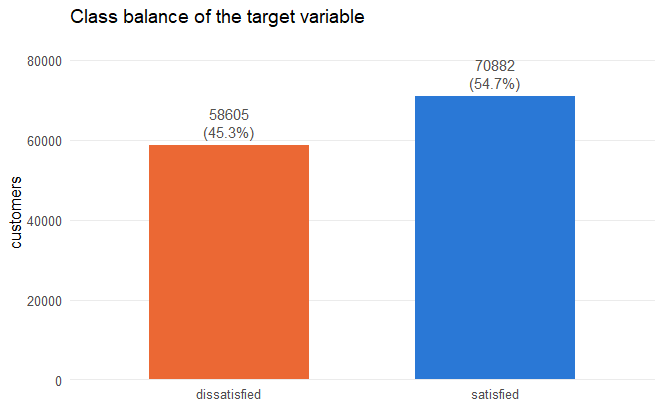
\includegraphics[width=0.4\linewidth]{img/data_expl/sat_balance.png}
    \caption{Target variable class balance}
    \label{img:sat_balance}
\end{figure}

To obtain a first indication of the relationship between the response variable and the remaining covariates, we examine their correlation, as shown in Fig.~\ref{img:full_corr}. Focusing on the service-quality variables (Fig.~\ref{img:qs_corr}), we can distinguish three subgroups of features. The correlation is computed using R's \texttt{corr()} function, which is based on Pearson's correlation coefficient
$$
r_{X,Y} = \frac{\sum (x_i - \bar{x})(y_i - \bar{y})}
               {\sqrt{\sum (x_i - \bar{x})^2 \sum (y_i - \bar{y})^2}}
$$
\begin{figure}
    \centering
    \begin{subfigure}[t]{.48\textwidth}
        \centering
        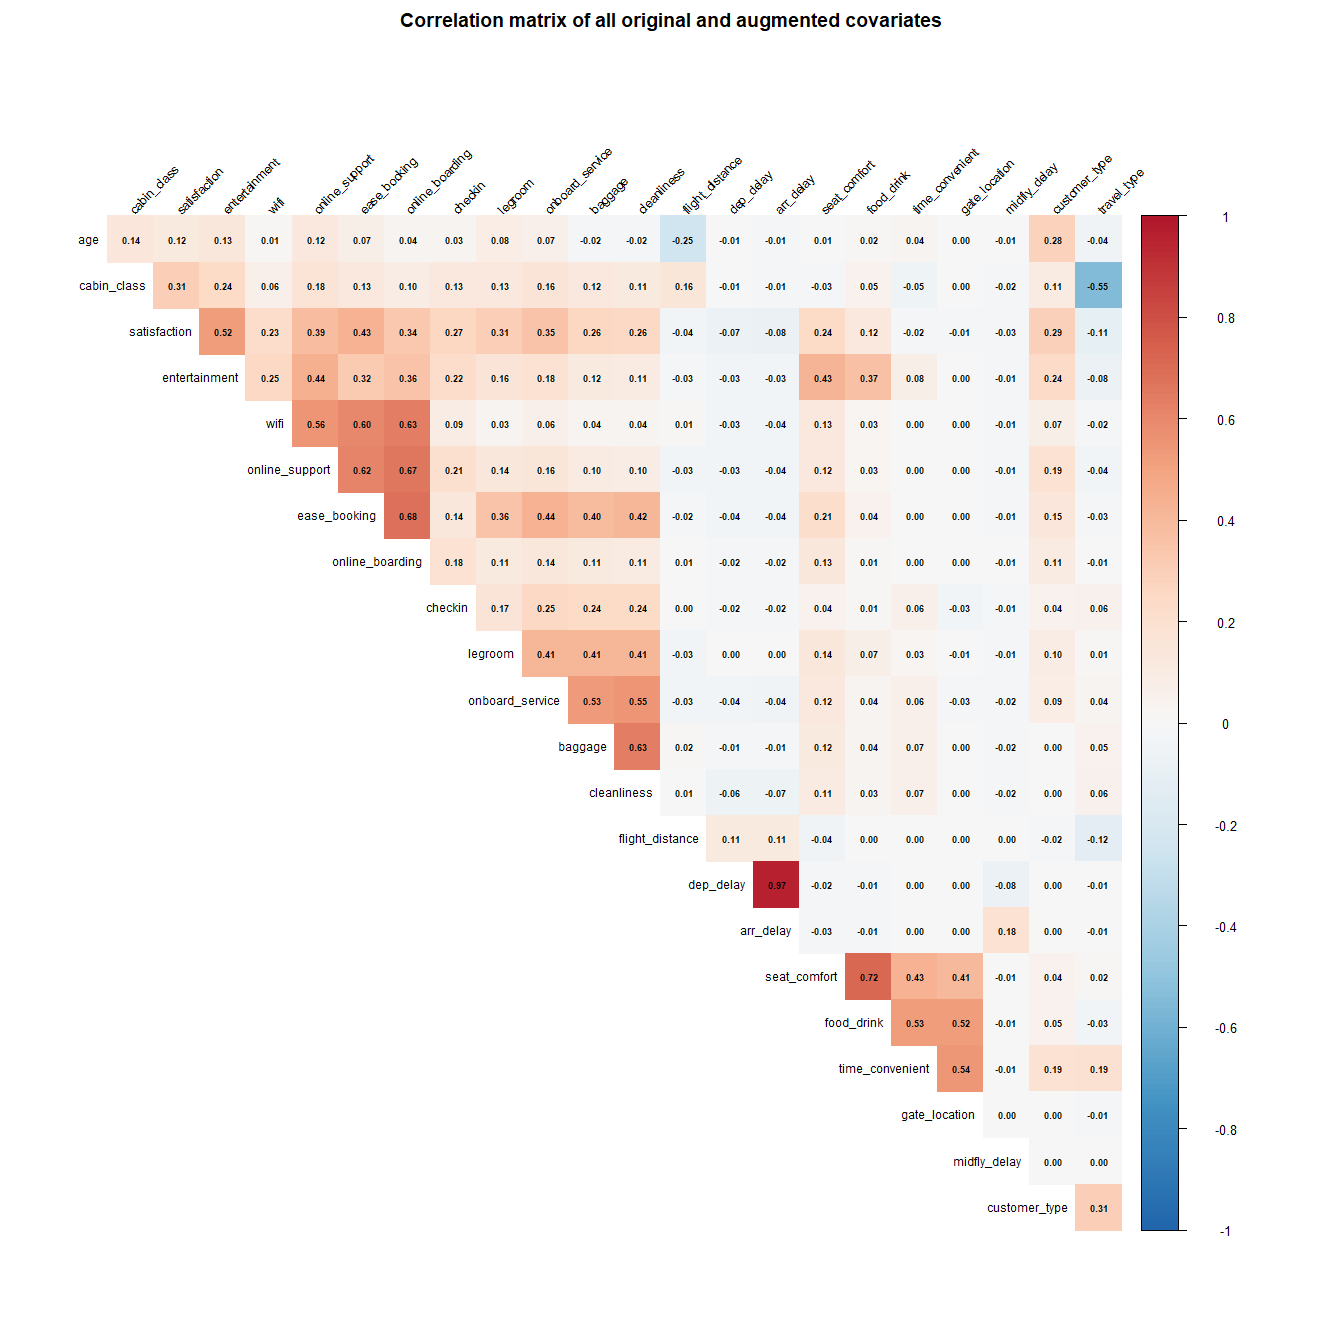
\includegraphics[width=\linewidth]{img/data_expl/full_corr.png}
        \caption{Correlation among all variables, both original and augmented}
        \label{img:full_corr}
    \end{subfigure}
    \hfill
    \begin{subfigure}[t]{.48\textwidth}
        \centering
        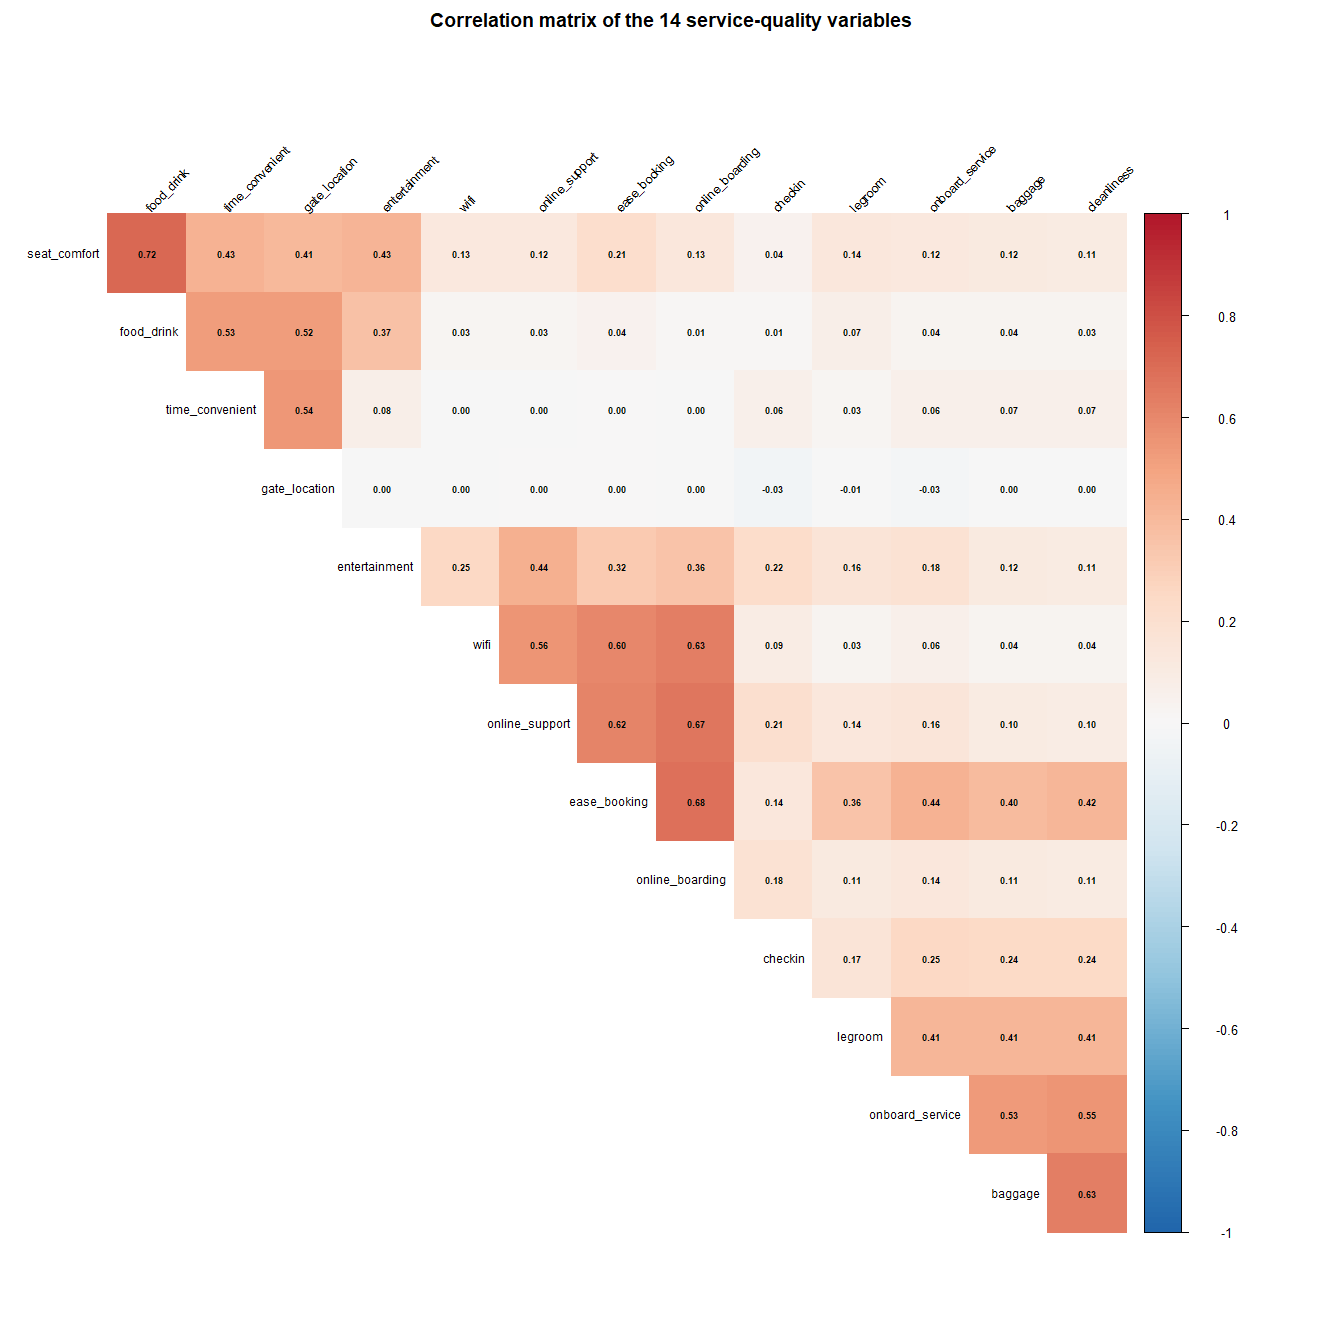
\includegraphics[width=\linewidth]{img/data_expl/qs_corr.png}
        \caption{Correlation among service-quality items}
        \label{img:qs_corr}
    \end{subfigure}
\end{figure}

Tab.~\ref{tab:class_balance} reports the class balance of the remaining categorical variables. Given the imbalance among their levels, we decided to stratify the train--test split of the dataset.
\begin{table}[htbp] 
  \centering
  \caption{Class balance of the categorical covariates}
  \label{tab:class_balance}
  \begin{tabular}{llr}
    \toprule
    Variable & Level & Proportion \\
    \midrule
    Satisfaction  & Dissatisfied      & 0.453 \\
                  & Satisfied         & 0.547 \\
    \addlinespace
    Customer type & Disloyal customer & 0.183 \\
                  & Loyal customer    & 0.817 \\
    \addlinespace
    Travel type   & Business travel   & 0.691 \\
                  & Personal travel   & 0.309 \\
    \addlinespace
    Cabin class   & Eco               & 0.449 \\
                  & Eco Plus          & 0.072 \\
                  & Business          & 0.479 \\
    \bottomrule
  \end{tabular}
\end{table}

\section{Model specification}
Let $y_i$ denote the satisfaction level of customer $i$. We assume that
$$
y_i \sim\ \textbf{Bernoulli}(p)
$$
where $p$ is the probability that a customer is satisfied.
We model the probability $p$ as a function of the covariates $X$ as
$$
\text{logit}(p)=\ln\left(\cfrac{p}{1-p}\right) = \beta_0+X\beta
$$
where $\beta_0$ is the intercept in the logit space and $\beta$ is the vector of regression coefficients of the covariates $X$ (after the introduction of midflight dely the deletion of arrival delay).
\newline
Later in the project we will carry out the analysis by using several models, and for each one of them we'll describe the structure of the prior we decide to use for the regression coefficients.


\section{Logit model}
\label{sec:logit}

In this chapter we present the results obtained by fitting a simple Bayesian
logistic regression on a reduced set of covariates. The aim is twofold: to
establish a first, fully interpretable baseline for the satisfaction
prediction problem introduced in Section \ref{sec:problem}, and to settle a
few modelling choices (prior specification, encoding of the cabin class, MCMC
setup) that will be reused by the richer shrinkage model of Section
\ref{sec:regression}.

\subsection{Covariates and model specification}
Following the suggestions of the brief, we fit the model on a compact subset of
covariates, using the transformations motivated in the data-exploration phase
(Section \ref{sec:data_expl}): \texttt{age}, \texttt{seat\_comfort},
\texttt{flight\_distance}, \texttt{cabin\_class}, the log-transformed departure
delay $\log(1+\texttt{dep\_delay})$ and the signed-log mid-flight delay, together
with the two binary descriptors \texttt{travel\_type} and
\texttt{customer\_type}. All continuous covariates are standardised
(zero mean, unit variance) so that coefficients are expressed per standard deviation and the common prior variance is equally informative for every covariate. For the binary covariates the reference
level is chosen as the majority group (\textit{Business travel} and
\textit{Loyal customer}), so that each coefficient measures the effect of the
minority condition relative to the typical customer.

Let $y_i \in \{0,1\}$ be the satisfaction outcome of customer $i$ (encoded as in
Section \ref{sec:problem}) and $x_i$ the corresponding row of the standardised
design matrix. We assume a Bernoulli likelihood with a logit link:
\begin{equation}
    y_i \mid p_i \sim \text{Bernoulli}(p_i),
    \qquad
    \text{logit}(p_i) = \beta_0 + x_i^\top \beta
        + \beta_{\text{mid}}\,\texttt{midflight\_delay}_i .
    \label{eq:logit_model}
\end{equation}
The mid-flight delay is deliberately kept outside the main design matrix and
given its own coefficient $\beta_{\text{mid}}$, paired with an explicit
per-row sampling statement $\texttt{midflight\_delay}_i \sim \mathcal{N}(0,1)$.
This treats the (standardised) mid-flight delay as a stochastic node rather than
a fixed regressor, which is convenient for handling it as an augmented quantity
and keeps its contribution cleanly separated from the other effects.

\paragraph{Prior specification.}
Since we have no strong prior belief on the magnitude or the sign of the
coefficients, and because standardisation already puts every covariate on a
comparable scale, we adopt independent, weakly informative Gaussian priors on
all the parameters:
\begin{equation}
    \beta_0 \sim \mathcal{N}(0, 100), \qquad
    \beta_j \sim \mathcal{N}(0, 100) \;\; (j = 1,\dots,P), \qquad
    \beta_{\text{mid}} \sim \mathcal{N}(0, 100).
    \label{eq:priors}
\end{equation}
Here the second argument denotes the prior \emph{variance} $\sigma^2 = 100$
(equivalently a precision $\tau = 1/\sigma^2 = 0.01$ in the JAGS
parametrisation). On the logit scale a standard deviation of $10$ is very
diffuse: it places essentially no informative constraint on plausible
coefficient values while still being proper, so the posterior is driven by the
likelihood, and the resulting estimates remain directly comparable to a
maximum-likelihood fit. This choice reflects our lack of prior information and
keeps the baseline model as neutral as possible.

\subsection{Encoding of the cabin class}
Before committing to the model we address a small preliminary question: is it
preferable to encode \texttt{cabin\_class} as a pair of dummy variables
(\textit{Eco Plus} and \textit{Business}, with \textit{Eco} as reference) or as a
single centred ordinal score ($1/2/3$)? To decide, we fit the model
\eqref{eq:logit_model} under both encodings and compare them with the Widely
Applicable Information Criterion (WAIC), computed from the pointwise
log-likelihood of the MCMC draws.

The dummy encoding attains the lower WAIC ($1373.2$ against $1379.6$ for the
ordinal one), i.e. a slightly better expected predictive fit. The difference in
expected log predictive density is $\Delta\text{elpd} = -3.2$ with a standard
error of $2.7$, so the preference, although real, is smaller than two standard
errors and therefore modest. Because \texttt{cabin\_class} is genuinely
\emph{nominal} rather than an equally-spaced ordinal scale, and because the
dummy specification is both more flexible and lets us report a separate,
directly interpretable odds ratio for each class, we adopt the dummy encoding
for the rest of the analysis.

\subsection{MCMC setup and convergence}
Posterior inference is carried out via MCMC in JAGS. We run $3$ parallel chains,
with an adaptation phase of $1500$ iterations, a burn-in of $1000$ iterations,
$3000$ monitored iterations per chain and a thinning factor of $7$ to reduce the
residual autocorrelation between consecutive draws. Table
\ref{tab:mcmc_settings} summarises these choices.

\begin{table}[htbp]
  \centering
  \caption{MCMC settings used for the logit model}
  \label{tab:mcmc_settings}
  \begin{tabular}{lr}
    \toprule
    Setting & Value \\
    \midrule
    Chains            & 3 \\
    Adaptation        & 1500 \\
    Burn-in           & 1000 \\
    Iterations (kept) & 3000 \\
    Thinning          & 7 \\
    \bottomrule
  \end{tabular}
\end{table}

Convergence was satisfactory for all parameters. The Gelman--Rubin potential
scale reduction factors are essentially $1$ (point estimates $1.00$--$1.01$,
upper confidence limits up to $1.02$, multivariate PSRF $= 1.01$), the trace
plots show well-mixed, stationary chains overlapping around a common region, and
the autocorrelation decays quickly to zero within a few lags after thinning. The
effective sample sizes range from about $590$ (for the intercept and the
personal-travel coefficient) to roughly $1350$, which is more than adequate for
stable posterior summaries. A complete convergence assessment
(trace plots, autocorrelation functions and the full diagnostic tables) is
deferred to Appendix \ref{app:mcmc_logit}.

\subsection{Posterior results}
Figures for the posterior densities of the coefficients and the odds-ratio
forest plot are collected below; the corresponding numerical summaries are
reported in Table \ref{tab:or_logit}. For each coefficient we report the
posterior mean, the $95\%$ credible interval on the log-odds scale
($\beta$) and the same quantities transformed to the odds-ratio scale
($\text{OR} = e^{\beta}$), which is the natural scale for interpretation.

% -----------------------------------------------------------------------------
% Figures intentionally omitted for now (text-only draft).
% Available knitted plots to insert later:
%   - Posterior densities, continuous coefficients (mcmc_areas group 1)
%   - Posterior densities, cabin-class dummies    (mcmc_areas group 2)
%   - Posterior densities, binary + intercept      (mcmc_areas group 3)
%   - Odds-ratio forest plot (95% credible intervals, log scale)
% -----------------------------------------------------------------------------

\begin{table}[htbp]
  \centering
  \caption{Posterior summaries of the logit coefficients and their odds ratios,
           sorted by decreasing OR. CIs are $95\%$ credible intervals.}
  \label{tab:or_logit}
  \resizebox{\linewidth}{!}{%
  \begin{tabular}{lrrrrrr}
    \toprule
    Term & $\bar\beta$ & $\beta_{2.5\%}$ & $\beta_{97.5\%}$ & OR & OR$_{2.5\%}$ & OR$_{97.5\%}$ \\
    \midrule
    Class: Business (vs Eco)             & $1.450$  & $1.120$  & $1.804$  & $4.265$ & $3.065$ & $6.075$ \\
    Seat comfort                         & $0.632$  & $0.485$  & $0.768$  & $1.881$ & $1.625$ & $2.156$ \\
    Class: Eco Plus (vs Eco)             & $0.050$  & $-0.441$ & $0.524$  & $1.052$ & $0.643$ & $1.688$ \\
    Age                                  & $-0.026$ & $-0.164$ & $0.127$  & $0.975$ & $0.848$ & $1.135$ \\
    Arrival delay residual (signed-log)  & $-0.041$ & $-0.187$ & $0.111$  & $0.960$ & $0.830$ & $1.118$ \\
    Flight distance                      & $-0.052$ & $-0.185$ & $0.090$  & $0.949$ & $0.831$ & $1.094$ \\
    Intercept                            & $-0.105$ & $-0.400$ & $0.180$  & $0.901$ & $0.670$ & $1.198$ \\
    Personal Travel (vs Business travel) & $-0.168$ & $-0.498$ & $0.166$  & $0.846$ & $0.608$ & $1.181$ \\
    $\log(1+\text{Departure Delay})$     & $-0.230$ & $-0.371$ & $-0.078$ & $0.795$ & $0.690$ & $0.925$ \\
    disloyal Customer (vs Loyal)         & $-1.825$ & $-2.253$ & $-1.431$ & $0.161$ & $0.105$ & $0.239$ \\
    \bottomrule
  \end{tabular}%
  }
\end{table}

\subsection{Interpretation}
Four effects clearly separate from the ``no-effect'' line (OR $=1$). By far the
largest is the cabin class: travelling in \textit{Business} rather than
\textit{Eco} multiplies the odds of being satisfied by roughly $4.3$
($95\%$ CI $[3.07, 6.08]$), even after adjusting for all the other covariates,
confirming the marginal contrast already seen in the data-exploration phase.
\textit{Seat comfort} is the strongest continuous driver
(OR $\approx 1.88$ per standard deviation, $[1.63, 2.16]$): more comfortable
seating is strongly associated with satisfaction. In the opposite direction, a
\textit{disloyal customer} has markedly lower odds of being satisfied
(OR $\approx 0.16$, $[0.11, 0.24]$), and a longer departure delay reduces them
too (OR $\approx 0.80$ per unit of $\log(1+\text{delay})$, $[0.69, 0.93]$).

The remaining covariates have credible intervals that comfortably include $1$
and cannot be called confident drivers on their own: \textit{Eco Plus} is
statistically indistinguishable from \textit{Eco}, while \textit{age},
\textit{flight distance} and the \textit{mid-flight delay residual} all show
weak, uncertain effects.

The most instructive case is the \textit{type of travel}. In the exploratory
analysis personal-travel customers appeared markedly less satisfied, an almost
certain marginal association; here, once cabin class and the other covariates
are held fixed, the credible interval for \textit{Personal Travel}
($0.61$ to $1.18$) comes close to, but no longer excludes, $1$. This is exactly
the confounding anticipated in Section \ref{sec:data_expl}: business travellers
are disproportionately booked in Business class, so once class enters the model
directly it absorbs most of the apparent travel-type effect. Both the borderline
effects (flight distance, departure delay) and this partially-explained
travel-type signal motivate the richer specification of Section
\ref{sec:regression}, where the full battery of $14$ service-quality ratings is
added under a shrinkage prior to clarify which of these effects survive
alongside the stronger, correlated service signals.

\section{Horseshoe shrinkage model}
\label{sec:regression}

\subsection{Motivation}
The logit model of Section \ref{sec:logit} was fit on the small set of
covariates suggested by the brief, taking their usefulness for granted. That is
a reasonable baseline, but it leaves open the central question of the analysis:
among \emph{all} the available predictors, in particular the fourteen
service-quality ratings that were set aside earlier, which ones actually carry
signal for customer satisfaction, and which are redundant? Rather than answering
this by hand, adding and removing covariates and guessing at their relevance, we
prefer a principled, automatic mechanism. We therefore fit a Bayesian logistic
regression on the \emph{full} set of covariates under a \textbf{horseshoe}
shrinkage prior \cite{bl_book}, which is designed to pull the coefficients of
noise predictors strongly towards zero while leaving genuine signals almost
untouched. This lets the data, rather than our prior guesses, single out the
meaningful covariates.

\subsection{Model specification}
We include all $21$ standardised predictors: the $14$ service-quality items
plus \texttt{age}, \texttt{flight\_distance}, the two cabin-class dummies
(\textit{Eco Plus}, \textit{Business}), $\log(1+\texttt{dep\_delay})$,
\textit{Personal Travel} and \textit{disloyal Customer} - and, as in Section
\ref{sec:logit}, the mid-flight delay is kept outside the design matrix with its
own coefficient $\beta_{\text{arr}}$. The likelihood is again Bernoulli with a
logit link:
\begin{equation}
    y_i \mid p_i \sim \text{Bernoulli}(p_i),
    \qquad
    \text{logit}(p_i) = \beta_0 + x_i^\top \beta
        + \beta_{\text{arr}}\,\texttt{arr\_delay}_i .
    \label{eq:hs_model}
\end{equation}

The horseshoe prior replaces the common vague Gaussian of Section
\ref{sec:logit} with a scale-mixture of normals: each coefficient gets its own
\emph{local} scale $\lambda_j$, and all local scales share a single
\emph{global} scale $\tau$,
\begin{equation}
    \beta_j \mid \lambda_j, \tau \sim \mathcal{N}(0, \lambda_j^2 \tau^2),
    \qquad
    \lambda_j \sim \mathcal{C}^+(0,1),
    \qquad
    \tau \sim \mathcal{C}^+(0,1),
    \label{eq:hs_prior}
\end{equation}
where $\mathcal{C}^+(0,1)$ denotes the standard half-Cauchy distribution. The
global scale $\tau$ pulls \emph{all} coefficients towards zero, enforcing overall
sparsity, while the heavy Cauchy tails of the local scales $\lambda_j$ let
individual coefficients escape that shrinkage when the data demand it - this is
precisely the ``a few large, most near zero'' behaviour that makes the prior
suited to feature selection. The arrival-delay coefficient
$\beta_{\text{arr}}$ is given its own local scale $\lambda_{\text{arr}}$ under
the \emph{same} global $\tau$, so that it competes for signal on an equal footing
with the other $21$ predictors. Following the JAGS notes, each half-Cauchy is
implemented as a Student-$t$ with one degree of freedom truncated to the positive
reals, \texttt{dt(0, 1, 1)\,T(0, )}. The intercept keeps a diffuse Gaussian
prior, $\beta_0 \sim \mathcal{N}(0, 100)$ (i.e. \texttt{dnorm(0, 0.01)}), and is
deliberately left out of the shrinkage so that the baseline log-odds is not
penalised.

A convenient by-product of the mixture form is the \emph{shrinkage weight}
\begin{equation}
    \kappa_j = \frac{1}{1 + \lambda_j^2},
    \qquad \kappa_j \in (0,1),
    \label{eq:kappa}
\end{equation}
which measures how much coefficient $j$ is pulled towards zero: $\kappa_j$ near
$0$ marks a preserved \emph{signal} (essentially unshrunk), whereas $\kappa_j$
near $1$ marks a coefficient shrunk towards \emph{noise}. We use the posterior
distribution of the $\kappa_j$ as our covariate-relevance summary.

\subsection{MCMC setup and convergence}
Because of the heavy-tailed half-Cauchy hyperpriors, the horseshoe posterior
mixes more slowly than the vague-prior model of Section \ref{sec:logit}, and it
is computationally heavier ($22$ coefficients, $22$ local scales and one global
scale, against the $9$ parameters of Section \ref{sec:logit}). We therefore
budget a longer sampling run and thinning from the outset; the settings, reported
in Table \ref{tab:hs_mcmc_settings}, are deliberately modest given the
single-core environment and could be extended on a larger machine.

Convergence was assessed separately for the two blocks of parameters, the
regression coefficients $\{\beta_j, \beta_0, \beta_{\text{arr}}\}$ and the scale
parameters $\{\lambda_j, \lambda_{\text{arr}}, \tau\}$, since the latter are the
harder to sample. For each block we inspected the Gelman--Rubin potential scale
reduction factors, the effective sample sizes, and the trace and autocorrelation
plots. The coefficients mix well and show scale-reduction factors close to $1$;
the scale parameters, and $\tau$ in particular, mix more slowly and show higher
autocorrelation, as expected for a horseshoe, but reach effective sample sizes
adequate for the summaries we report. Figures \ref{fig:hs_trace_beta} and
\ref{fig:hs_trace_lambda} show a representative trace plot for each block. The
complete diagnostic material - all trace and autocorrelation plots for both the
$\beta$ and the $\lambda$ parameters, together with the full Gelman--Rubin and
effective-sample-size tables - is collected in Appendix
\ref{app:mcmc_horseshoe}.

\subsection{Posterior results}
Figure \ref{fig:hs_posterior} shows the marginal posterior densities of the
coefficients: most concentrate tightly around zero, with only a handful clearly
displaced, which is the visual signature of the shrinkage at work. The relevance
ranking is made explicit in Figure \ref{fig:hs_shrinkage}, which plots the
posterior distribution of the shrinkage weights $\kappa_j$ of
Eq.~\eqref{eq:kappa}: predictors on the ``signal'' side ($\kappa_j$ small) are
the ones the model retains, while those pushed to $\kappa_j \to 1$ are treated as
redundant. Figure \ref{fig:hs_forest} reports the same information on the
coefficient scale, as a forest plot of the posterior means and $95\%$ credible
intervals of the $\beta_j$, colouring in the covariates identified as signal
($\kappa_j < 0.5$).

\begin{figure}[htbp]
\centering
\begin{subfigure}[t]{0.48\linewidth}
  \centering
  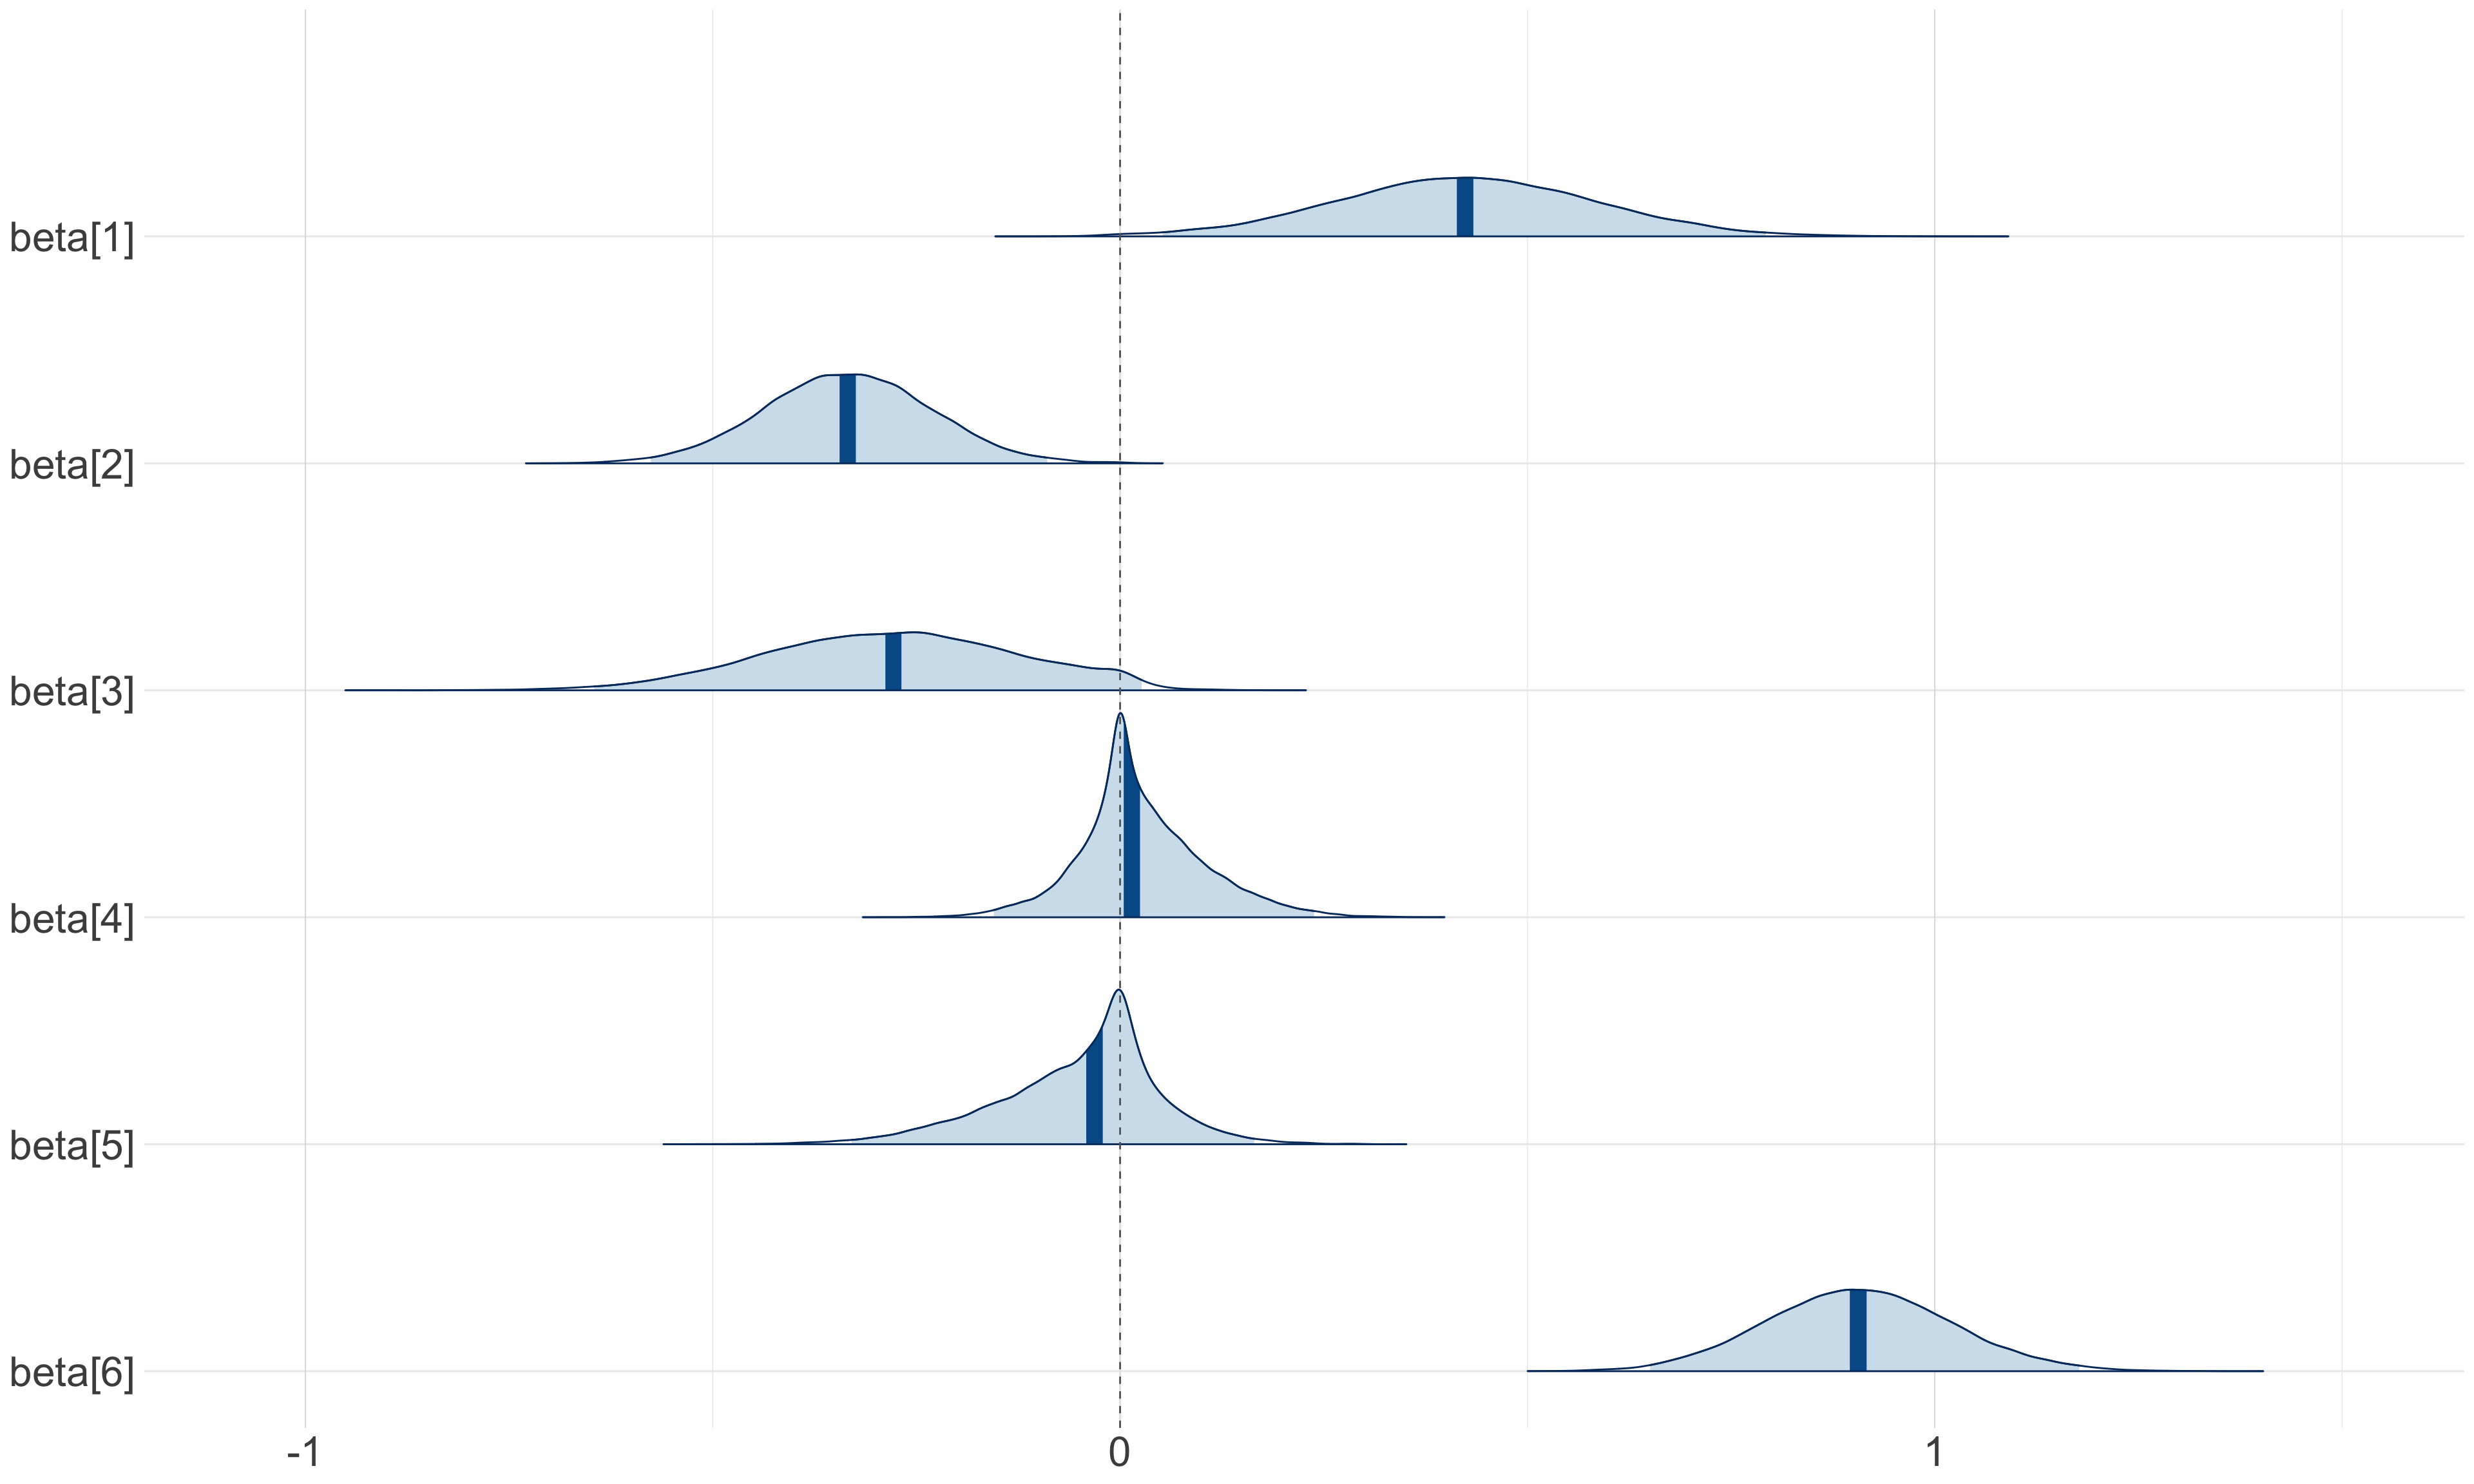
\includegraphics[width=\linewidth]{img/horseshoe_model/post1.png}
  \caption{Marginal posterior densities of the coefficients under the horseshoe
           prior ($98\%$ intervals). Most coefficients are shrunk tightly around
           zero; only a few escape.}
  \label{fig:hs_posterior}
\end{subfigure}\hfill
\begin{subfigure}[t]{0.48\linewidth}
  \centering
  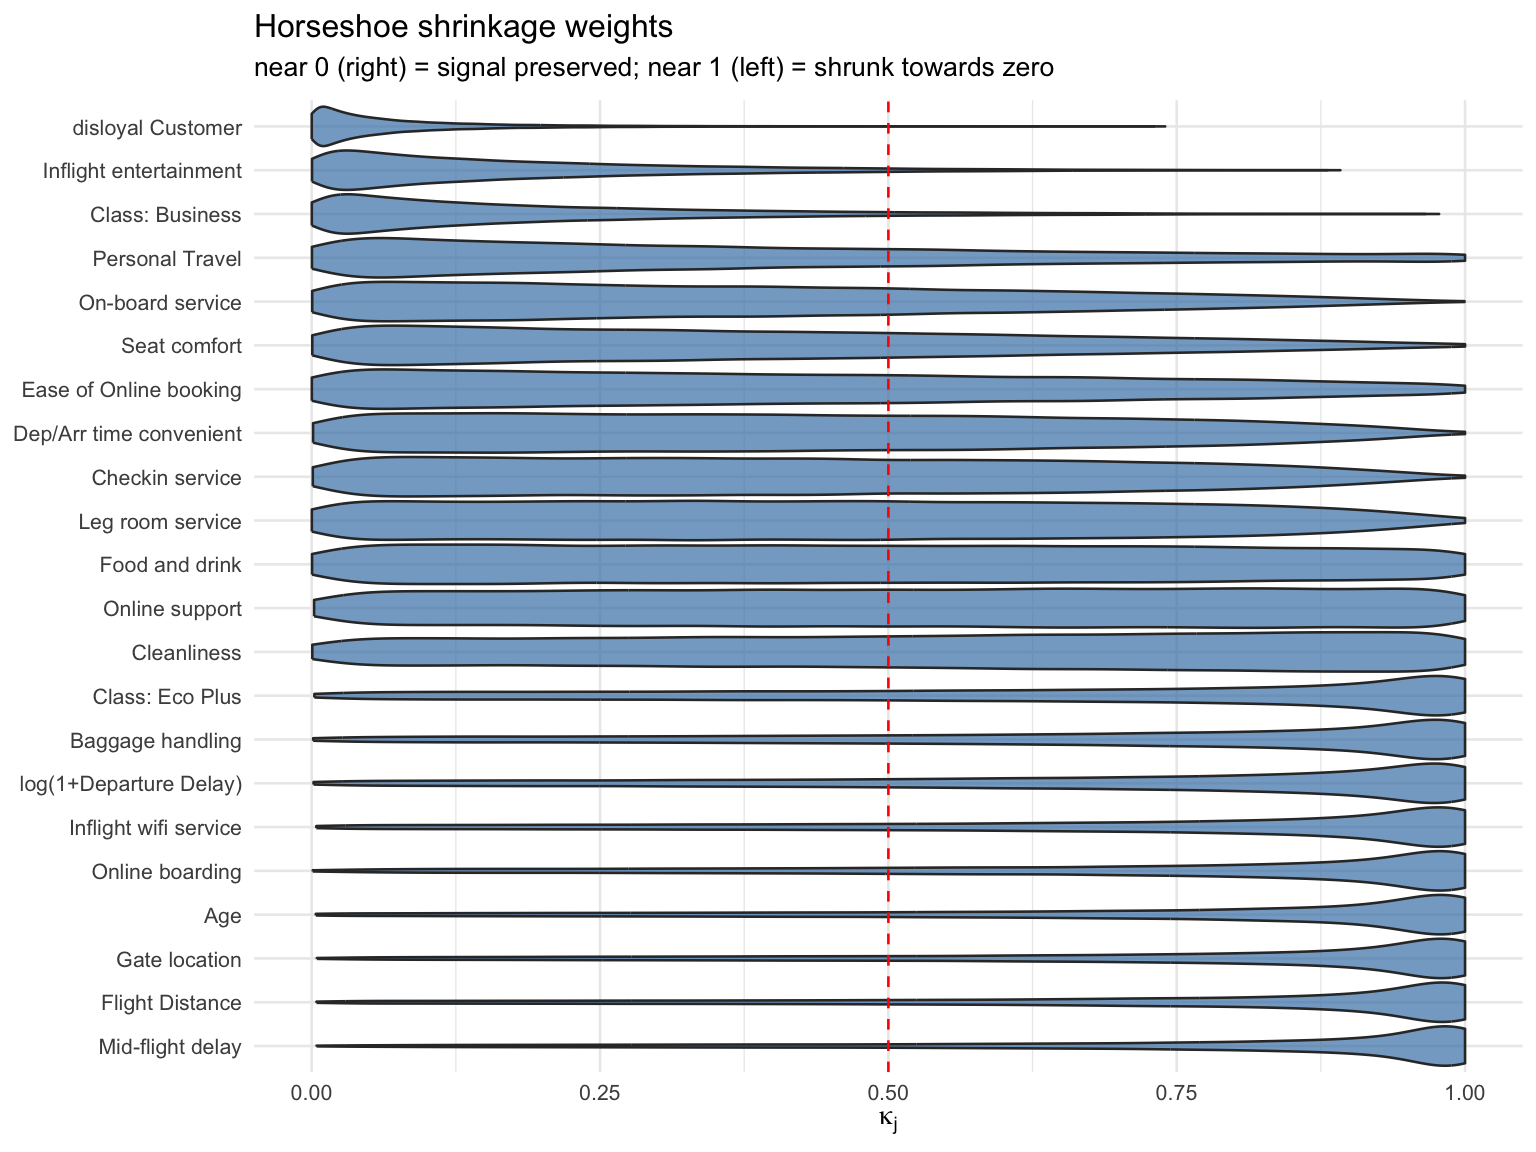
\includegraphics[width=\linewidth]{img/horseshoe_model/shrinkage_beta.png}
  \caption{Posterior distribution of the horseshoe shrinkage weights $\kappa_j$
           for each predictor. Near $0$ (right) the signal is preserved; near $1$
           (left) the coefficient is shrunk towards zero. The dashed line marks
           $\kappa_j = 0.5$.}
  \label{fig:hs_shrinkage}
\end{subfigure}
\end{figure}

\begin{figure}[htbp]
  \centering
  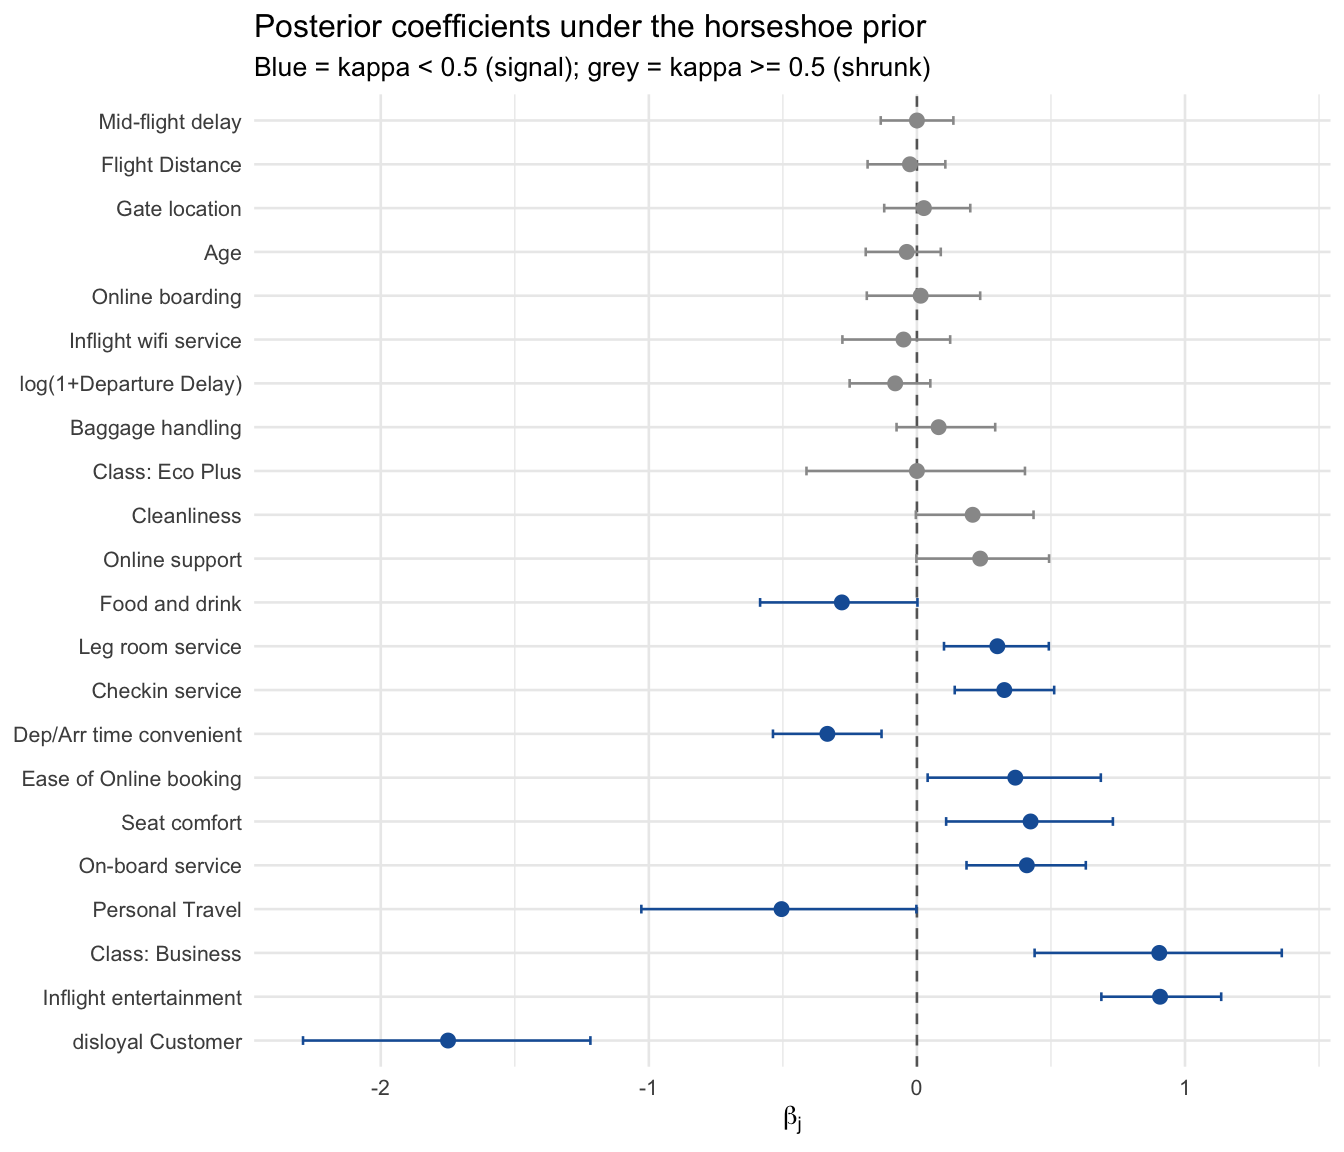
\includegraphics[width=0.75\linewidth]{img/horseshoe_model/beta_forest.png}
  \caption{Posterior coefficients $\beta_j$ under the horseshoe prior (means and
           $95\%$ credible intervals). Blue marks the covariates identified as
           signal ($\kappa_j < 0.5$), grey the shrunk ones.}
  \label{fig:hs_forest}
\end{figure}

\subsection{Conclusions}
The horseshoe cleanly separates the informative predictors from the redundant
ones, and several of its findings sharpen - and in one case reverse - the
picture from Sections \ref{sec:data_expl} and \ref{sec:logit}.

\paragraph{The booking / connectivity cluster visibly competes.}
Among the four mutually correlated ``booking / connectivity'' items identified in
the exploratory analysis (Section \ref{sec:data_expl}), the prior does not treat
them symmetrically: \textit{Ease of Online booking} and \textit{Online support}
are preserved noticeably more than \textit{Online boarding} and
\textit{Inflight wifi service} - the latter being the single most shrunk item in
the whole model. This is exactly the mechanism the horseshoe was chosen for: when
several correlated items carry overlapping information, the prior lets two of them
represent the signal and treats the other two as largely redundant, instead of
forcing us to pick one by hand.

\paragraph{Business class shrinks once service quality is in the model.}
In Section \ref{sec:logit}, \textit{Business} class alone carried a large,
confident odds ratio (about $4$). Here, with all $14$ service ratings included,
its coefficient shrinks markedly and its credible interval crosses zero. The
natural reading is \emph{mediation}, not disappearance: Business passengers are
more satisfied largely \emph{because} they enjoy better seat comfort,
entertainment and service, so in Section \ref{sec:logit} the \textit{Class}
dummy was partly standing in for those ratings simply because they were not yet
in the model.

\paragraph{Personal Travel gets stronger, not weaker.}
Section \ref{sec:logit} found the type-of-travel effect nearly explained away by
\textit{Class}. Under the horseshoe, once the service ratings control for the
\emph{quality} of the trip experience, \textit{Personal Travel} re-emerges as one
of the strongest and most confidently negative effects in the model, with a
credible interval lying entirely below zero. The two findings are not
contradictory: they show that the earlier attenuation was specifically about
\textit{Class} soaking up part of the travel-type signal, not about travel type
being unimportant.

\paragraph{A cautionary sign on time convenience.}
More tentatively, \textit{Departure/Arrival time convenient} has a
\emph{negative} posterior mean with a credible interval excluding zero - higher
ratings associated with \emph{lower} satisfaction, which is counter-intuitive.
Recall from Section \ref{sec:data_expl} that this item has one of the largest
shares of structural zeros and sits in its own correlated cluster with
\textit{Seat comfort}, \textit{Food and drink} and \textit{Gate location}; its
zeros plausibly encode ``not applicable'' rather than genuine dissatisfaction.
We therefore read this coefficient as a candidate symptom of that ambiguity
rather than a reliable substantive finding, and revisit it directly in the
structural-zero robustness check of Section \ref{sec:robustness}.

\paragraph{Loyalty dominates throughout.}
Finally, \textit{disloyal Customer} remains, by a wide margin, the single
strongest and most confidently preserved effect in the entire model - consistent
across the exploratory analysis and both models of Sections \ref{sec:logit} and
\ref{sec:regression}, regardless of how many other covariates are present.

% -----------------------------------------------------------------------------
% NOTE: the .Rmd conclusions quote exact posterior figures via inline `r ...`
% code (specific kappa_j values, the Business/Personal-Travel/time-convenient
% posterior means and 95% credible-interval endpoints). Those numbers come from
% the knitted run and were not available when this draft was written, so they
% are described qualitatively above. Fill in the precise values from the
% kappa_tbl of notebook 03 (03_horseshoe_summary.rds) where desired.
% -----------------------------------------------------------------------------

% ------------------------------------------------------------------
\section{Prior Sensitivity and Structural Robustness}
\label{sec:sensitivity}
% ------------------------------------------------------------------
This section stress-tests the conclusions of Sections~\ref{sec:logit}
and~\ref{sec:regression} against four choices made along the way: the prior
variance of the vague model, the global scale of the horseshoe, the treatment
of the ambiguous structural-zero rows, and the size of the training set. Each
check requires a full JAGS refit, so they are run by separate scripts
(\texttt{04a}--\texttt{04d}) whose stored output is read back here.

% ==================================================================
\subsection{Logit model prior sensitivity}
\label{sec:sens-logit}
% ==================================================================
We refit the model of Section~\ref{sec:logit} four times, varying only the
prior variance on every $\beta_j$: $\sigma^2_\beta \in \{1, 10, 100, 10000\}$.
Figure~\ref{fig:prior-sweep} overlays the resulting posterior means and $95\%$
credible intervals, and Table~\ref{tab:prior-range} gives the range each
posterior mean covers across the four fits.

\begin{figure}[htbp]
\centering
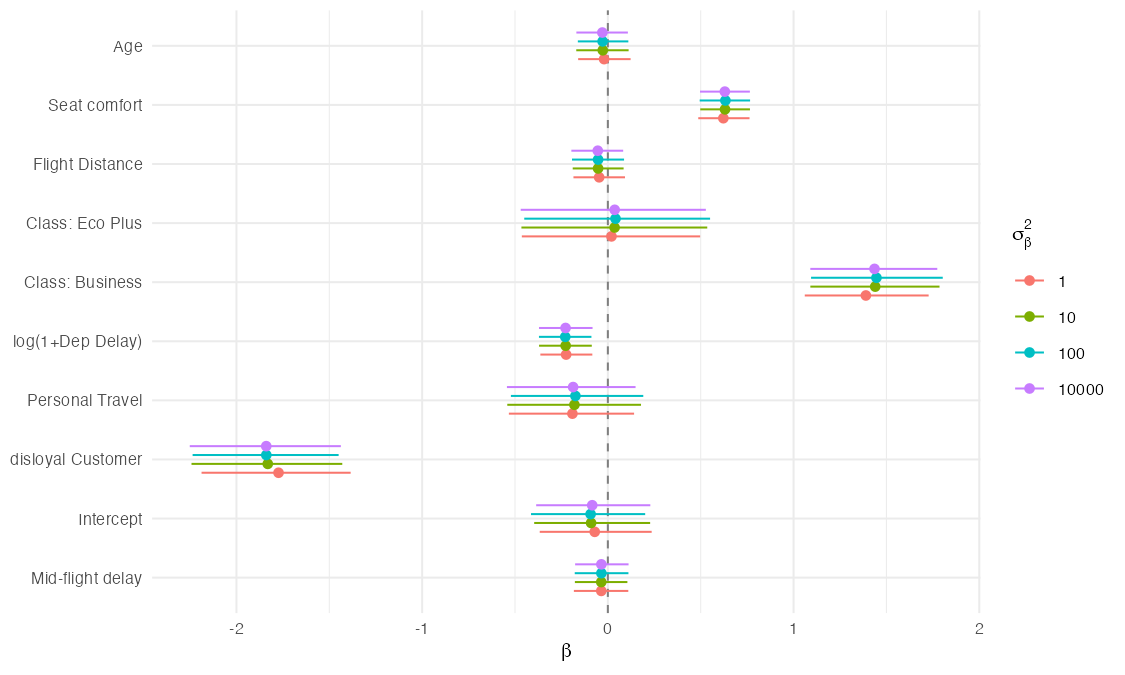
\includegraphics[width=0.85\linewidth]{img/sensitivity/prior_sweep.png}
\caption{Posterior coefficients of the vague-prior logit model across four
prior variances.}
\label{fig:prior-sweep}
\end{figure}

\begin{table}[htbp]
\centering
\caption{Range of posterior means across the four prior variances.}
\label{tab:prior-range}
\begin{tabular}{lc}
\toprule
Term & Range of posterior mean \\
\midrule
disloyal Customer             & 0.066 \\
Class: Business               & 0.057 \\
Intercept                     & 0.022 \\
Class: Eco Plus               & 0.022 \\
Personal Travel               & 0.016 \\
Seat comfort                  & 0.011 \\
Age                           & 0.009 \\
Flight Distance               & 0.008 \\
log(1+Departure Delay)        & 0.005 \\
Mid-flight delay (signed-log) & 0.001 \\
\bottomrule
\end{tabular}
\end{table}

Across four orders of magnitude of prior variance the largest movement is
$0.066$ on the log-odds scale, for a coefficient whose posterior mean is itself
of order $1$--$2$. At $n \approx 1200$ the likelihood dominates every prior we
tested, so the vague-prior results are not an artefact of the variance we
happened to pick.

% ==================================================================
\subsection{Horseshoe prior sensitivity}
\label{sec:sens-horseshoe}
% ==================================================================
The horseshoe's behaviour is governed by the scale $s$ of the half-Cauchy
prior on the global scale, $\tau \sim \mathcal{C}^+(0,s)$: small $s$ pulls
every coefficient towards zero, large $s$ relaxes the shrinkage. It is the one
hyperparameter whose value could plausibly change \emph{which} covariates the
model keeps, so it is the one worth testing. We refit the
Section~\ref{sec:regression} model at $s \in \{0.1, 1, 10\}$, holding the local
scales $\lambda_j$ at $\mathcal{C}^+(0,1)$, and recompute the shrinkage weights
$\kappa_j = 1/(1+\lambda_j^2)$.

\begin{figure}[!ht]
\centering
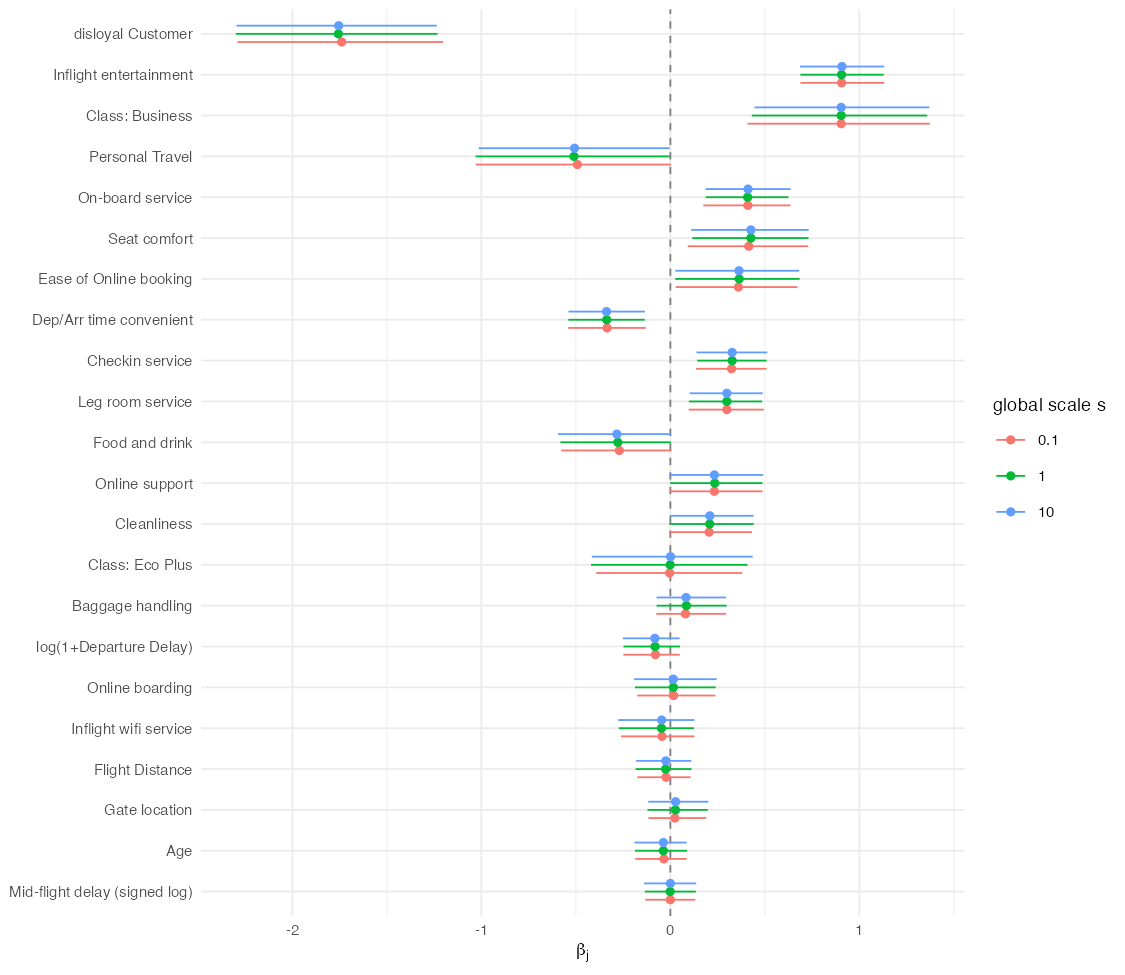
\includegraphics[width=0.62\linewidth]{img/sensitivity/horseshoe_sweep.png}
\caption{Horseshoe posterior coefficients across three global scales, ordered
by shrinkage weight at the default scale.}
\label{fig:hs-beta}
\end{figure}

Across this hundred-fold range exactly one of the $22$ predictors changes its
signal/noise verdict, and no posterior mean moves by more than $0.018$; the
per-predictor weights are tabulated in Appendix~\ref{app:mcmc_horseshoe}. The
strong effects of Section~\ref{sec:regression} remain strong and confidently
non-zero at every scale. What little drift there is sits among coefficients
already on the $\kappa = 0.5$ boundary, which is where sensitivity to $s$ is
expected and where we drew no firm conclusions in the first place.

% ==================================================================
\subsection{Structural-zero robustness check}
\label{sec:sens-structzero}\label{sec:robustness}
% ==================================================================
Section~\ref{sec:regression} raised the possibility that the negative
coefficient on \texttt{Departure/Arrival time convenient} is an artefact of the
structural zeros flagged in Section~\ref{sec:data_expl}, that is, of zeros
meaning ``not applicable'' rather than genuine dissatisfaction. Refitting the
horseshoe model without those rows drops $110$ records and leaves $1103$.

\begin{table}[htbp]
\centering
\caption{Horseshoe refit excluding structural-zero rows. Only the predictors
kept as signal ($\kappa_j < 0.5$) are shown; the full table is in
Appendix~\ref{app:mcmc_horseshoe}.}
\label{tab:structzero}
\begin{tabular}{lcccc}
\toprule
Term & $\beta$ mean & $\beta$ lo & $\beta$ hi & $\kappa_j$ \\
\midrule
Disloyal Customer              & $-2.286$ & $-2.975$ & $-1.599$ & 0.059 \\
Inflight entertainment         & $+1.090$ & $+0.833$ & $+1.361$ & 0.165 \\
Class: Business                & $+0.976$ & $+0.387$ & $+1.535$ & 0.199 \\
Seat comfort                   & $+0.881$ & $+0.577$ & $+1.194$ & 0.209 \\
Personal Travel                & $-0.641$ & $-1.278$ & $-0.008$ & 0.331 \\
On-board service               & $+0.521$ & $+0.231$ & $+0.798$ & 0.338 \\
Dep/Arr time convenient        & $-0.513$ & $-0.782$ & $-0.234$ & 0.347 \\
Ease of Online booking         & $+0.493$ & $+0.090$ & $+0.902$ & 0.370 \\
Checkin service                & $+0.378$ & $+0.154$ & $+0.595$ & 0.420 \\
Leg room service               & $+0.297$ & $+0.056$ & $+0.529$ & 0.486 \\
\bottomrule
\end{tabular}
\end{table}

The hypothesis does not survive. The coefficient does not shrink towards zero
once the ambiguous rows are removed; it becomes \emph{more} negative, from
$-0.335$ to $-0.513$, with a slightly wider interval as expected with $110$
fewer records. Whatever drives the effect, it is not the structural-zero
ambiguity we suspected, and we report it as an open finding rather than force a
tidier story onto it.

The other two members of that correlated cluster move in opposite directions.
\texttt{Seat comfort} strengthens, $\kappa$ falling from $0.367$ to $0.209$ and
$\beta$ rising from $+0.419$ to $+0.881$, while \texttt{Food and drink} goes
from a borderline signal ($\kappa = 0.492$, $\beta = -0.275$) to firmly shrunk
($\kappa = 0.733$, $\beta = +0.020$). The structural zeros therefore do not add
uniform noise across the cluster; they affect its members differently.

% ==================================================================
\subsection{Sample-size robustness}
\label{sec:sens-samplesize}
% ==================================================================
The checks above varied the prior and which rows enter the fit; this one varies
how many. Every model in this report is estimated on \num{1213} records,
following the project brief, which supplies a 1000-customer subset of the
original data for exactly this purpose. Refitting the model of
Section~\ref{sec:logit} on a stratified subsample of \num{15003} records leaves
the coefficients we rely on unmoved, \texttt{Class: Business} by $0.005$,
\texttt{disloyal Customer} by $0.014$ and \texttt{Seat comfort} by $0.022$, and
contracts the credible intervals by a median factor of $3.42$ against the
$3.52$ that $\sqrt{n}$ asymptotics predicts. Three weak effects
(\texttt{Flight Distance}, \texttt{Age}, \texttt{Mid-flight delay}) acquire
intervals excluding zero, which is a limitation of the $n = 1213$ analysis
rather than a finding about the airline.

% ==================================================================
% Prediction and validation --- includable fragment
% Numbers come from 06_prediction_validation.Rmd.
% ==================================================================

\providecommand{\TODO}[1]{\textbf{[TODO: #1]}}
\providecommand{\figplaceholder}[1]{%
  \framebox[0.8\textwidth]{%
    \parbox[c][4cm][c]{0.75\textwidth}{\centering\itshape #1}}}

% ------------------------------------------------------------------
\section{Prediction and validation}
\label{sec:prediction}
% ------------------------------------------------------------------
Everything up to this point has been estimated on the \num{1213}-customer
training subsample. This section confronts the model with the \num{128274}
held-out customers set aside in Section~\ref{sec:problem}, which were never
used for fitting, standardisation or variable selection. Following the
conclusion of Section~\ref{sec:sensitivity}, the horseshoe model is the one
carried forward here; the corresponding comparison against the vague-prior
logit and against BAS is reported in Appendix~\ref{app:bas_vs_hs}.

\subsection{From posterior draws to predicted probabilities}
For a held-out customer with covariate row $\tilde{x}_i$, the Bayesian point
prediction is the posterior mean of the success probability, obtained by
pushing every retained draw through the inverse link and averaging:
\begin{equation}
  \hat{p}_i \;=\;
  \frac{1}{S}\sum_{s=1}^{S}
  \operatorname{logit}^{-1}\!\Bigl(
      \beta_0^{(s)} + \tilde{x}_i^{\top}\beta^{(s)}
      + \beta_{\text{mid}}^{(s)}\,\texttt{midflight\_delay}_i
  \Bigr),
  \label{eq:postpred}
\end{equation}
This averages the transformed draws rather than transforming the averaged
ones: $\operatorname{logit}^{-1}$ is non-linear, so
$\mathbb{E}[g(\theta)] \neq g(\mathbb{E}[\theta])$, and only the former
propagates posterior uncertainty. Test covariates are standardised with the
\emph{training} means and standard deviations, so nothing from the held-out
set enters the fit.

\subsection{Discrimination and probabilistic accuracy}
We report two complementary summaries. The area under the ROC curve (AUC)
measures how well the model \emph{ranks} customers and is invariant to the
cutoff. The Brier score,
\begin{equation}
  \mathrm{BS} \;=\; \frac{1}{n}\sum_{i=1}^{n}\bigl(\hat{p}_i - y_i\bigr)^2 ,
  \label{eq:brier}
\end{equation}
is a strictly proper scoring rule, minimised only when the stated
probabilities match the true ones, so it rewards predictions that are both
well ranked and numerically honest. On the held-out set the horseshoe model
attains an AUC of $0.900$ and a Brier score of $0.126$.

\subsection{Classification and the choice of cutoff}
Turning probabilities into hard classifications requires a cutoff.
Table~\ref{tab:pred-cutoff} contrasts the conventional $0.5$ with the training
base rate $\bar{y} = 0.546$, the natural alternative when the two classes are
not perfectly balanced.

\begin{table}[htbp]
\centering
\small
\caption{Classification performance on the held-out set at two cutoffs.}
\label{tab:pred-cutoff}
\setlength{\tabcolsep}{4pt}
\begin{tabular}{lccc}
\toprule
Cutoff & Sensitivity & Specificity & Accuracy \\
\midrule
$t = 0.5$              & 0.837 & 0.812 & 0.826 \\
$t = \bar{y} = 0.546$  & 0.815 & 0.843 & 0.828 \\
\bottomrule
\end{tabular}
\end{table}

Moving to the base rate trades about two points of sensitivity for three of
specificity and leaves accuracy essentially unchanged ($0.826$ against
$0.828$). That near-indifference is informative: the errors are not
concentrated on one side, and accuracy alone is a blunt instrument for
choosing an operating point. The right cutoff depends on what the two mistakes
cost, which is Section~\ref{sec:pred-loss}.

\subsection{Calibration}
Neither AUC nor accuracy asks whether the predicted probabilities \emph{mean}
what they claim: among customers the model calls $70\%$ likely to be satisfied,
roughly $70\%$ should be. This matters as much as discrimination here, since
the posterior predictive probability is the object we report.
Table~\ref{tab:calibration} bins the held-out set into deciles of predicted
probability against the observed rate.


Calibration is good in the upper half: from the seventh decile up, predicted
and observed agree closely ($0.801$ against $0.819$, $0.896$ against $0.937$).
In the middle the model is mildly over-confident about dissatisfaction,
predicting $0.33$ and $0.49$ in deciles four and five where the observed rates
are $0.26$ and $0.43$, and the lowest two deciles reverse that. So the model
separates the classes well at the extremes, where most predictions live, and
is least trustworthy around $\hat{p} \approx 0.3$--$0.6$, where the evidence
genuinely is ambiguous.

\begin{table}[htbp]
\centering
\small
\caption{Calibration by decile of predicted probability.}
\label{tab:calibration}
\setlength{\tabcolsep}{4pt}
\begin{tabular}{cccc}
\toprule
Decile & Mean predicted & Observed rate & $n$ \\
\midrule
1  & 0.035 & 0.122 & \num{12828} \\
2  & 0.100 & 0.125 & \num{12827} \\
3  & 0.195 & 0.163 & \num{12827} \\
4  & 0.326 & 0.260 & \num{12828} \\
5  & 0.489 & 0.430 & \num{12827} \\
6  & 0.658 & 0.637 & \num{12827} \\
7  & 0.801 & 0.819 & \num{12828} \\
8  & 0.896 & 0.937 & \num{12827} \\
9  & 0.946 & 0.984 & \num{12827} \\
10 & 0.977 & 0.997 & \num{12828} \\
\bottomrule
\end{tabular}
\end{table}

\subsection{Posterior predictive check by subgroup}
\label{sec:pred-ppc}
The checks above compare point predictions against outcomes. A posterior
predictive check asks more: taking the fitted model seriously as a generative
description and simulating whole replicated datasets from it, do those
replications reproduce features of the real data the fit never targeted? For
each posterior draw we simulate outcomes for the entire held-out set and
recompute the satisfaction rate within each level of \texttt{Class},
\texttt{Customer Type} and \texttt{Type of Travel}, giving a posterior
predictive distribution per subgroup, shown in Figure~\ref{fig:ppc}, to
compare the observed rate against.

\begin{figure}[htbp]
\centering
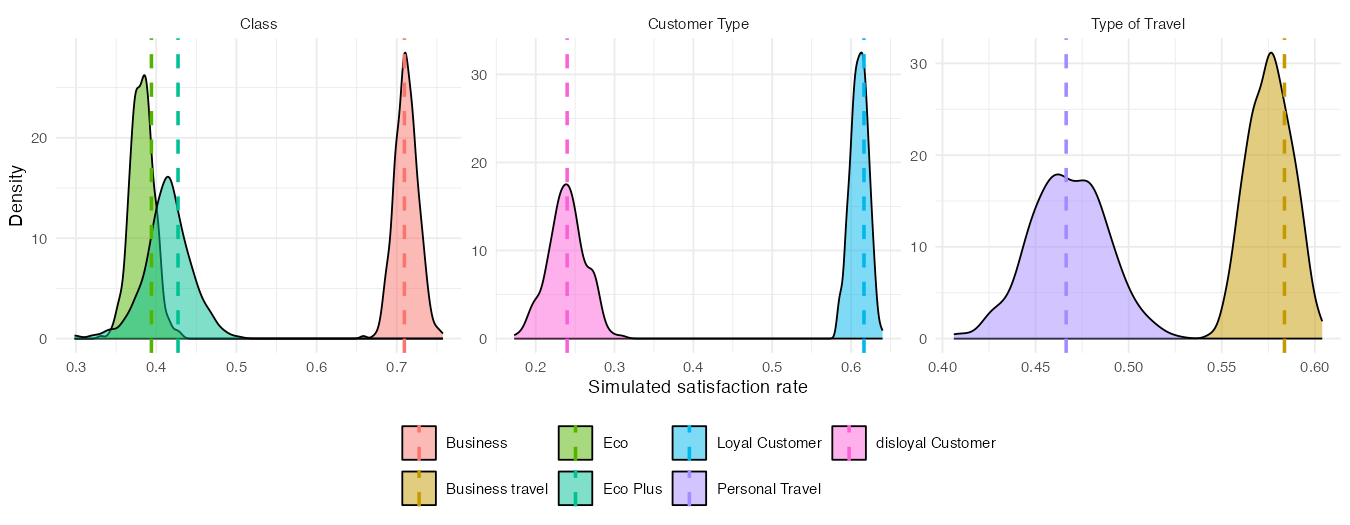
\includegraphics[width=0.75\linewidth]{img/prediction/ppc_subgroups.png}
\caption{Posterior predictive check by subgroup. Densities are the simulated
satisfaction rates; dashed lines mark the rates actually observed in the
held-out set.}
\label{fig:ppc}
\end{figure}

The observed rates fall inside the bulk of the simulated distributions for
every subgroup of all three variables, so the model is not systematically over-
or under-predicting satisfaction for any class of customer on data it has
never seen. The subgroup rates were never fitted directly, so reproducing them
is evidence that the covariate effects were captured rather than merely tuned
to the aggregate.

\subsection{Choosing the cutoff by expected loss}
\label{sec:pred-loss}
Rather than pick $0.5$ or the ROC-optimal point by convention, we state what
the two errors cost and minimise posterior expected loss. The airline flags a
customer when $\hat{p}_i < t$ and follows up with a retention contact; write
$C_{\text{miss}}$ for the cost of missing a dissatisfied customer and
$C_{\text{waste}}$ for that of contacting a satisfied one. The expected loss
at cutoff $t$ is
\begin{equation}
  \mathcal{L}(t) \;=\;
  C_{\text{miss}} \cdot \mathbb{P}\bigl(\hat{p} \ge t,\; y = 0\bigr)
  \;+\;
  C_{\text{waste}} \cdot \mathbb{P}\bigl(\hat{p} < t,\; y = 1\bigr),
  \label{eq:loss}
\end{equation}
estimated on the held-out set. Only the \emph{ratio} of the costs matters, so
the airline need not price either error, just say how many wasted contacts it
would trade for one retained customer. Table~\ref{tab:loss} gives the optimum
at three such ratios.

\begin{table}[htbp]
\centering
\small
\caption{Cutoff minimising expected loss, by assumed cost ratio
$C_{\text{miss}}\!:\!C_{\text{waste}}$.}
\label{tab:loss}
\setlength{\tabcolsep}{4pt}
\begin{tabular}{lcc}
\toprule
Cost ratio & Optimal cutoff $t^\star$ & Expected loss \\
\midrule
$1\!:\!1$ (equal cost) & 0.56 & 0.172 \\
$3\!:\!1$              & 0.74 & 0.252 \\
$5\!:\!1$              & 0.80 & 0.287 \\
\bottomrule
\end{tabular}
\end{table}

Under equal costs the optimum is $t^\star = 0.56$, essentially the base rate
and close to the conventional $0.5$, a useful sanity check on
Equation~\eqref{eq:loss}. As missing a dissatisfied customer grows more
expensive the cutoff rises, to $0.74$ at $3\!:\!1$ and $0.80$ at $5\!:\!1$: the
airline flags far more customers, accepting wasted contacts to catch the
recoverable ones. This is where the Bayesian machinery pays off operationally.
Because the model returns a calibrated distribution rather than a label, the
same fit supports any cost structure the business specifies, and the cutoff
follows from the loss function instead of convention.

% ==================================================================
\section{Conclusions}
\label{sec:conclusions}
% ==================================================================
We modelled airline customer satisfaction with a Bernoulli-logit likelihood,
first on the reduced covariate set suggested by the brief and then on the full
set under a horseshoe shrinkage prior, with \texttt{BAS} model averaging as an
independent cross-check. All posteriors were sampled by MCMC in JAGS.

Three effects dominate and survive every specification. Customer loyalty is the
strongest by a wide margin and the least shrunk coefficient at every global
scale tested; \emph{Inflight entertainment} and \emph{Business} class follow,
essentially tied ($\kappa_j = 0.17$ and $0.19$). Entertainment is the service
item the prior preserves most clearly, while \emph{Inflight wifi service} is
heavily shrunk despite correlating at $0.67$ with \emph{Online boarding} inside
the same booking cluster. That asymmetry is what the horseshoe was chosen for.

These conclusions are not artefacts of our modelling choices. The vague-prior
posterior moves by at most $0.066$ across four orders of magnitude of prior
variance; one predictor of twenty-two changes its signal/noise verdict across a
hundred-fold range of the global scale, and it sits on the $\kappa = 0.5$
boundary; and a training set twelve times larger moves the coefficients we
report by at most $0.022$. Out of sample, on \num{128274} unseen customers, the
model reaches an AUC of $0.900$, classifies $82.8\%$ correctly, and reproduces
the observed satisfaction rate in every subgroup.

One result resisted explanation: \emph{Departure/Arrival time convenient}
carries a negative coefficient whose interval excludes zero, and refitting
without the structural-zero rows strengthened it rather than weakening it, so
we report it as an open question. Three limitations are worth naming. The
structural zeros were flagged and tested but not modelled with a zero-inflated
likelihood; $n \approx 1200$ is modest for twenty-two predictors, which is why
several effects are borderline.


\begin{appendices}
\section{Data augmentation} \label{app:data_aug}

\subsection{Decorrelating departure and arrival delays}
Inspecting the correlation matrix (Fig.~\ref{img:full_corr}), we notice an extremely high correlation between \texttt{Departure delay} and \texttt{Arrival delay}. This value makes the two variables almost duplicates of one another. In order to remove this redundancy while retaining as much information as possible, we decided to replace Arrival delay with a quantity that captures the difference between the two.

We considered two options:
\begin{itemize}
    \item using the plain difference between the two variables;
    \item fitting a simple linear regression model with \texttt{Arrival delay} as the target and \texttt{Departure delay} as the covariate, and taking the residual of each observation as the new covariate.
\end{itemize}
The second model is more general and, in fact, encompasses the first one; however, the first is more interpretable and carries an immediate meaning, such as ``mid-flight delay'' or ``time gained during the flight''. The deciding point was whether the second option differed enough from the first to justify its higher complexity.

The regression model that reproduces the plain difference is the one with slope equal to 1 and intercept equal to 0. Fitting the regression model on the full dataset yields an intercept of 0.76 and a slope of 0.97; we therefore decided to opt for the simple difference between the arrival and departure delays.

\subsection{Reducing covariates skewness}
From the boxplots in Fig.\ref{fig:boxplot_skew} we can see how covariates \texttt{Flight Distance}, \texttt{Departure Delay} and \texttt{Mid-flight delay} are extremelly right-skewed. Since covariate skewnes might slow down MCMC convergence and are prone to present outliers and leverage points, we decided to transform them and check whether the transformation is beneficial.
\begin{figure}[h]
    \centering
    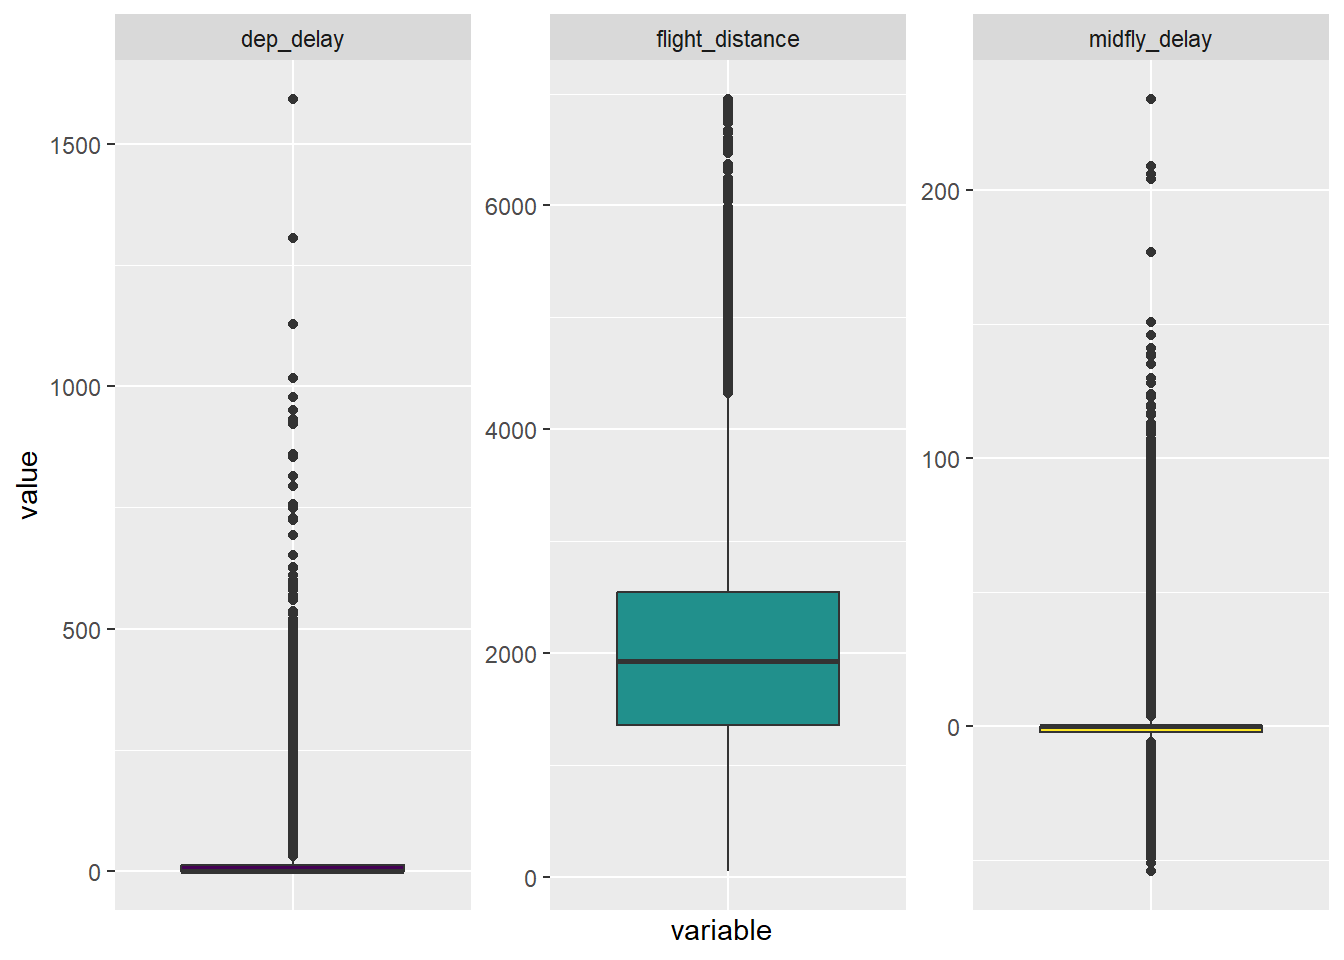
\includegraphics[width=0.5\linewidth]{img//data_expl/boxplot_skew.png}
    \caption{Boxplots of skewed covariates.}
    \label{fig:boxplot_skew}
\end{figure}

Since both \texttt{Flight distance} and \texttt{Departure delay} are non-negative we transform them using $ln(1+x)$; instead for \texttt{Mid-flight delay} we use the \textit{signed-log transformation} $\text{sign}(x)    \cdot ln(1+|x|)$ due the presence of negative values.
\begin{table}[ht]
\centering
\begin{tabular}{lr}
\hline
\textbf{variable} & \textbf{skewness} \\
\hline
Flight Distance & 0.466 \\
log1p(Flight Distance) & -1.599 \\
Departure Delay & 6.853 \\
log1p(Departure Delay) & 0.919 \\
Midflight Delay & 2.941 \\
signed-log(Midflight delay) & 0.234 \\
\hline
\end{tabular}
\caption{Skewness of raw and transformed variables}
\label{tab:skewness}
\end{table}

As we can see in Tab.~\ref{tab:skewness} \texttt{Flight distance} is only midly skewed and the transformation actually turn to be worse than the original varibale, therefore we kept it unchanged. Instead for what concerns \texttt{Departure delay} and \texttt{Mid-flight delay} we see higher level of skewness and the transformation improves this aspect; therefore we decided to kee the log-transformed variables.


\section{Low-informative logit model MCMC convergence} \label{app:logit_convergence}
The following section reports the plots and indices used to asses the convergence of our MCMC used to esitame the simple logit model shown in Section \ref{sec:logit}. In \

\begin{figure}[h]
    \centering
    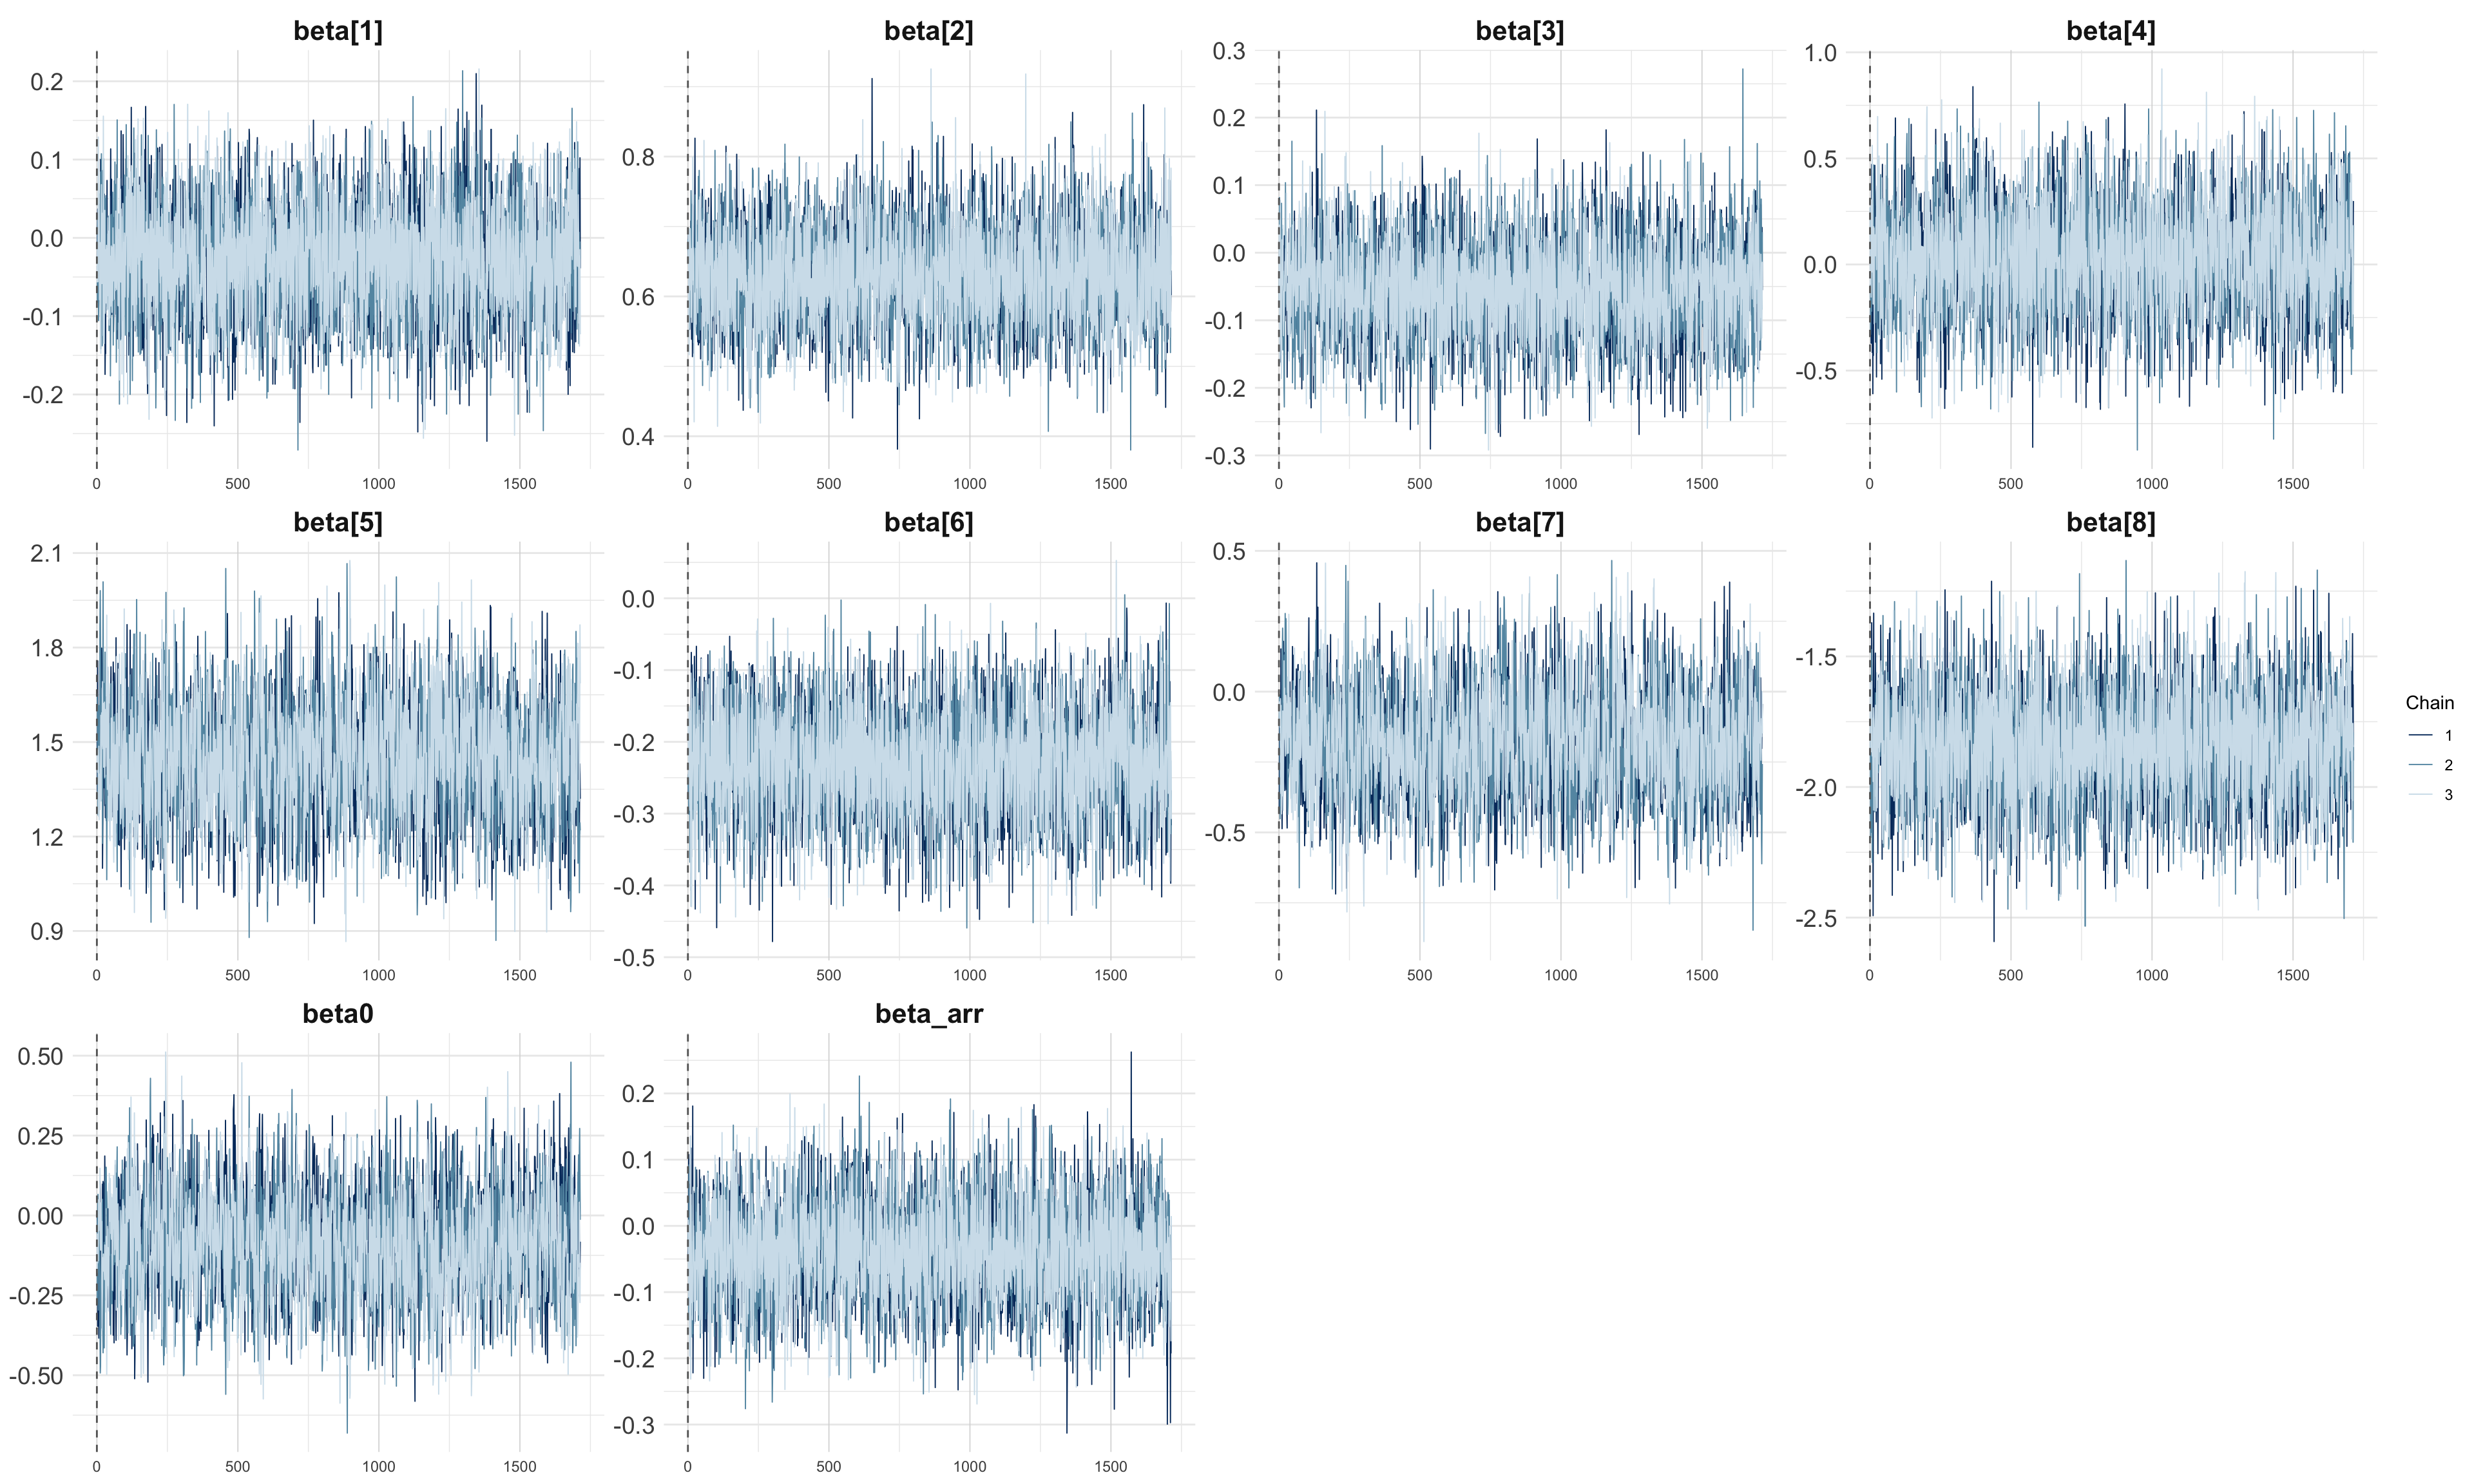
\includegraphics[width=0.9\linewidth]{img/logit_model/trace.png}
    \caption{MCMC traceplot of the baseline logit model.}
    \label{fig:logit_trace}
\end{figure}

\begin{figure}[h]
    \centering
    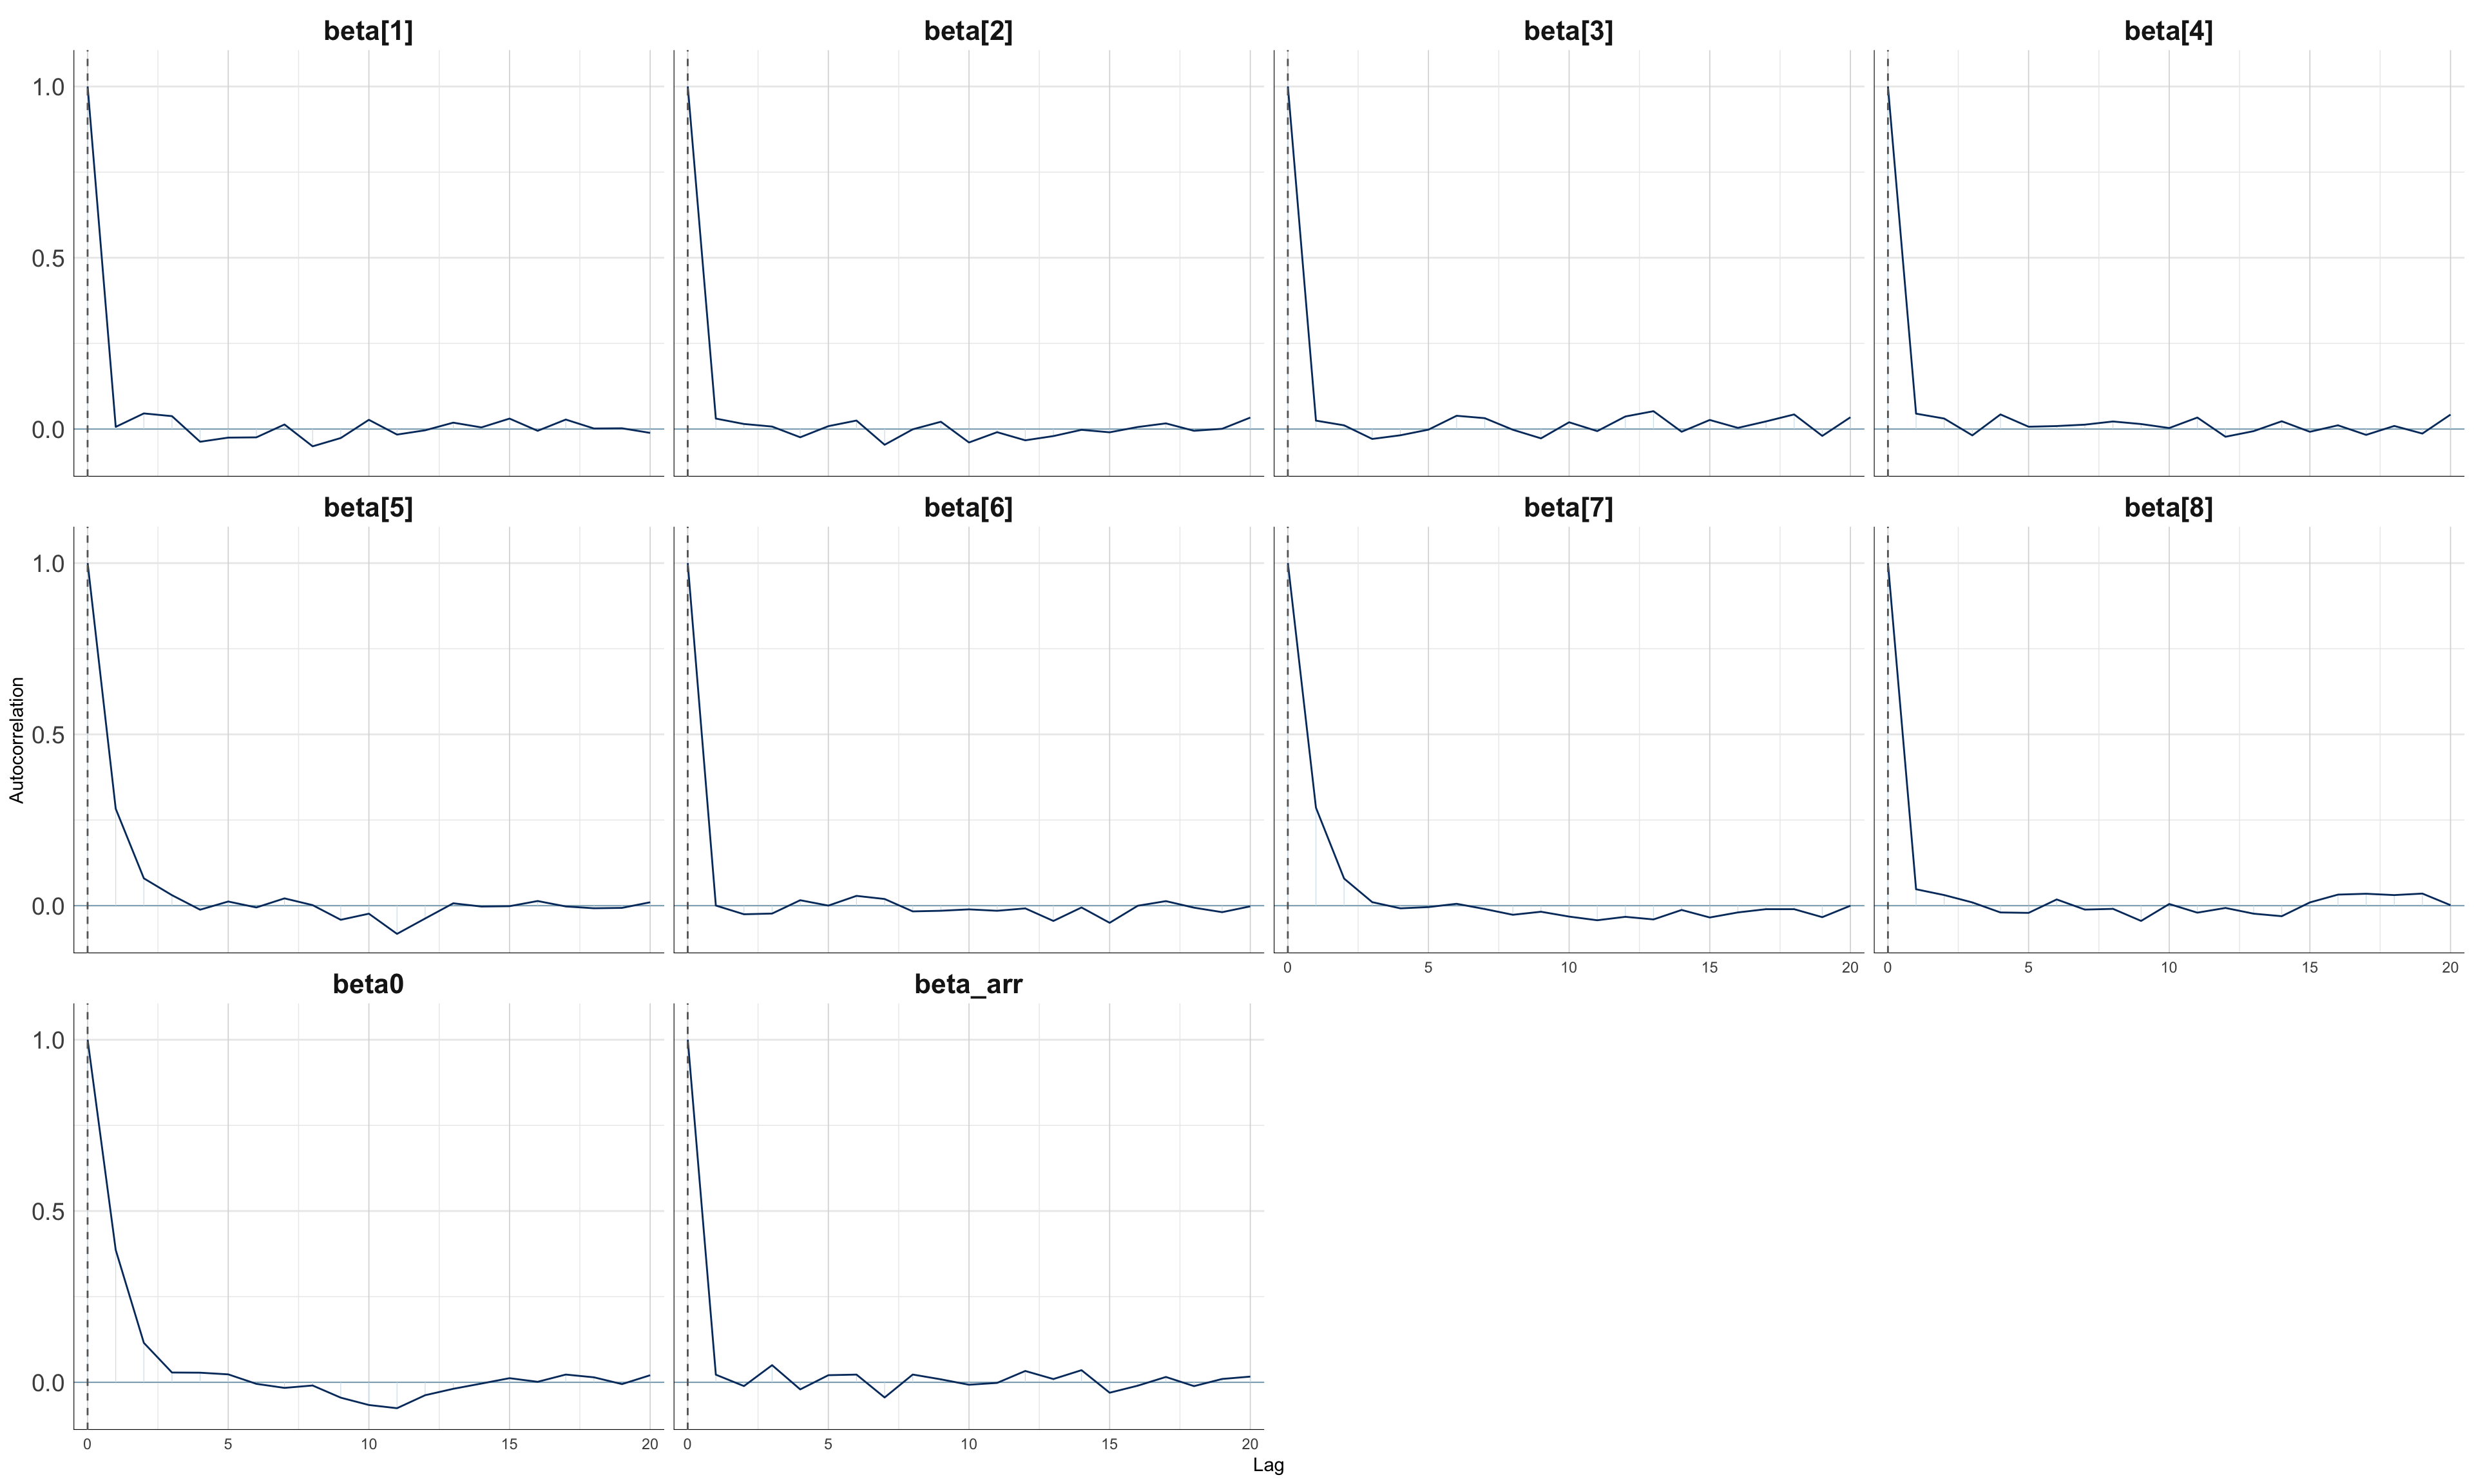
\includegraphics[width=0.7\linewidth]{img/logit_model/acf_1.png}
    \caption{MCMC ACF plots of the baseline logit model (1st chain).}
    \label{fig:logit_acf1}
\end{figure}

\begin{figure}[h]
    \centering
    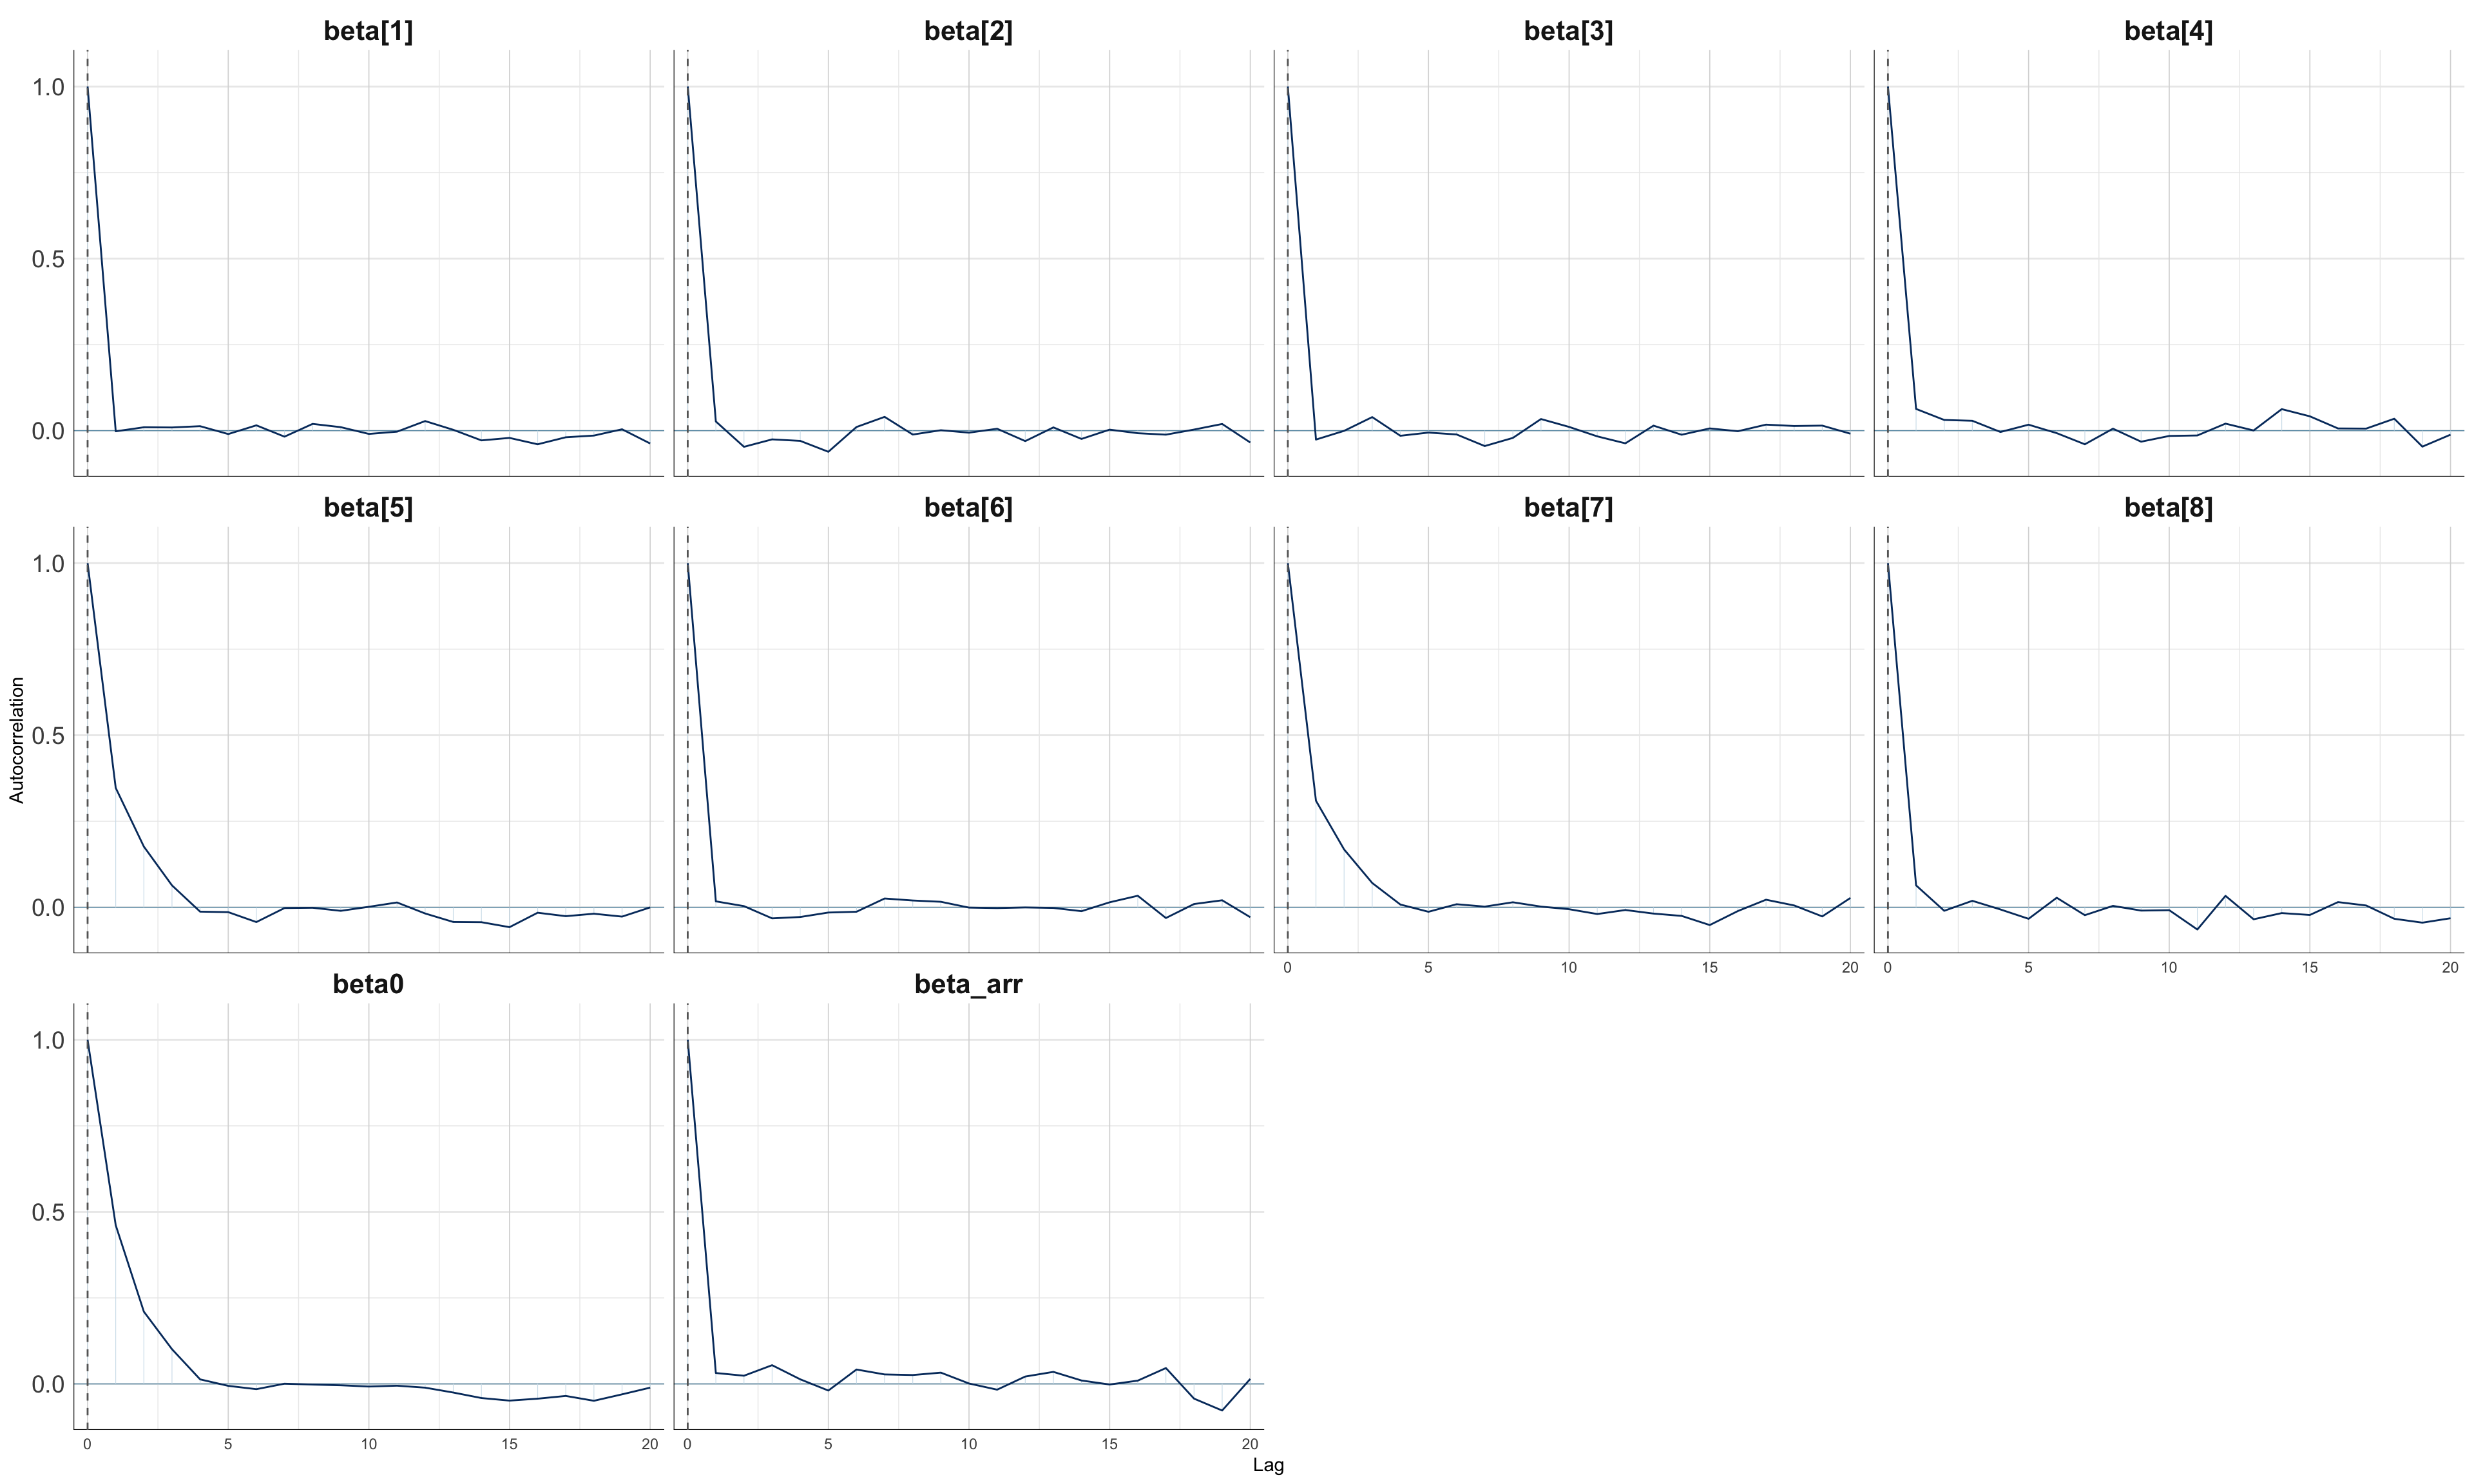
\includegraphics[width=0.7\linewidth]{img/logit_model/acf_2.png}
    \caption{MCMC ACF plots of the baseline logit model (2nd chain).}
    \label{fig:logit_acf2}
\end{figure}

\begin{figure}[h]
    \centering
    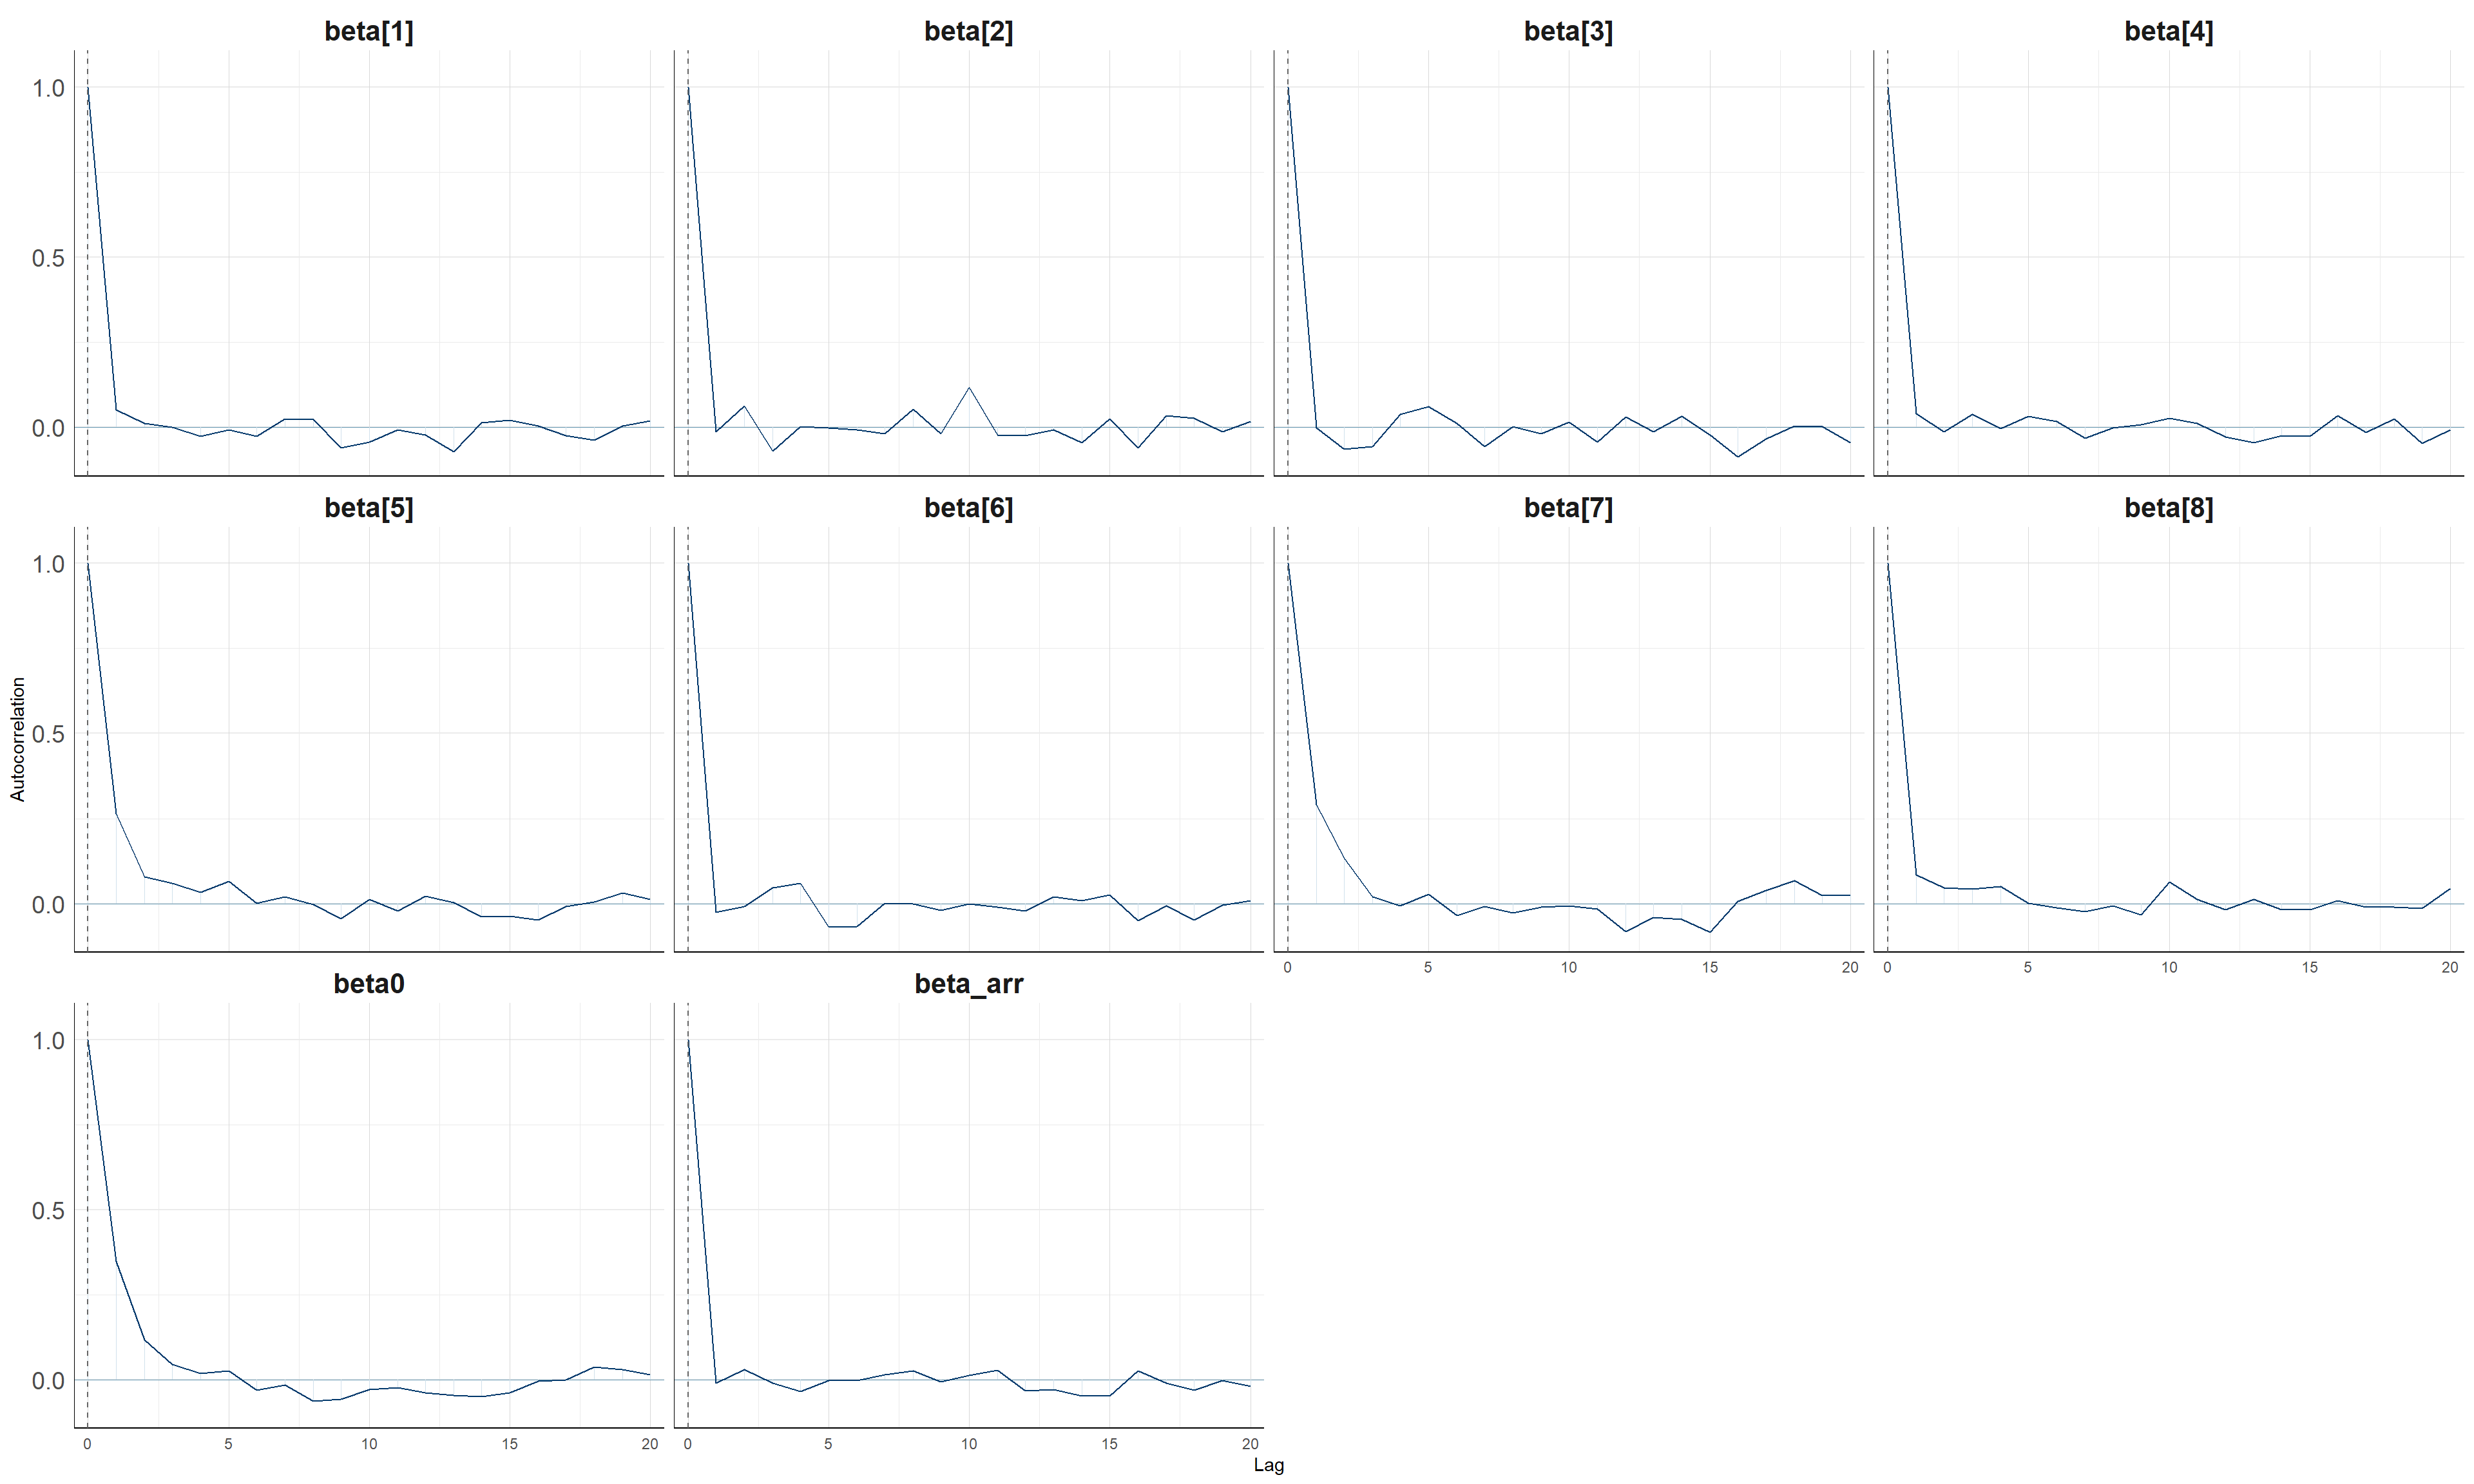
\includegraphics[width=0.7\linewidth]{img/logit_model/acf_3.png}
    \caption{MCMC ACF plots of the baseline logit model (3rd chain).}
    \label{fig:logit_acf3}
\end{figure}

\begin{table}[htbp]
  \centering
  \begin{minipage}[t]{0.48\textwidth}
    \centering
    \captionof{table}{Gelman--Rubin potential scale reduction factors.}
    \label{tab:psrf}
    \begin{tabular}{l S[table-format=1.2] S[table-format=1.2]}
      \toprule
      Parameter & {Point est.} & {Upper C.I.} \\
      \midrule
      $\beta_{1}$      & 1 & 1.00 \\
      $\beta_{2}$      & 1 & 1.00 \\
      $\beta_{3}$      & 1 & 1.00 \\
      $\beta_{4}$      & 1 & 1.01 \\
      $\beta_{5}$      & 1 & 1.00 \\
      $\beta_{6}$      & 1 & 1.01 \\
      $\beta_{7}$      & 1 & 1.00 \\
      $\beta_{8}$      & 1 & 1.01 \\
      $\beta_{0}$      & 1 & 1.01 \\
      $\beta_{\text{arr}}$ & 1 & 1.00 \\
      \midrule
      \multicolumn{3}{l}{\footnotesize Multivariate PSRF: 1} \\
      \bottomrule
    \end{tabular}
  \end{minipage}
  \hfill
  \begin{minipage}[t]{0.48\textwidth}
    \centering
    \captionof{table}{Effective sample sizes.}
    \label{tab:ess}
    \begin{tabular}{l S[table-format=4.3]}
      \toprule
      Parameter & {ESS} \\
      \midrule
      $\beta_{1}$      & 2486.772 \\
      $\beta_{2}$      & 2600.655 \\
      $\beta_{3}$      & 2799.333 \\
      $\beta_{4}$      & 2279.599 \\
      $\beta_{5}$      & 1324.157 \\
      $\beta_{6}$      & 3331.237 \\
      $\beta_{7}$      & 1253.960 \\
      $\beta_{8}$      & 2028.591 \\
      $\beta_{0}$      & 1123.153 \\
      $\beta_{\text{arr}}$ & 2571.000 \\
      \bottomrule
    \end{tabular}
  \end{minipage}
\end{table}

\section{Horseshoe model MCMC convergence} \label{app:horseshoe_convergence}
This appendix collects the diagnostics behind the convergence claims made in
Section~\ref{sec:regression} for the horseshoe model. Three chains,
\num{30000} retained draws each after a burn-in of \num{1000} and thinning of
$3$. Diagnostics are reported separately for the two blocks of parameters:
the regression coefficients $\{\beta_j, \beta_0, \beta_{\text{mid}}\}$ and the
scale parameters $\{\lambda_j, \lambda_{\text{mid}}, \tau\}$, the latter being
the harder to sample.

\subsection*{Trace plots}
Figures~\ref{fig:hs_trace_beta} and~\ref{fig:hs_trace_lambda} in
Section~\ref{sec:regression} show the first group of each block. The remaining
groups follow.
\begin{figure}[htbp]
  \centering
  \begin{subfigure}[t]{0.48\linewidth}
    \centering
    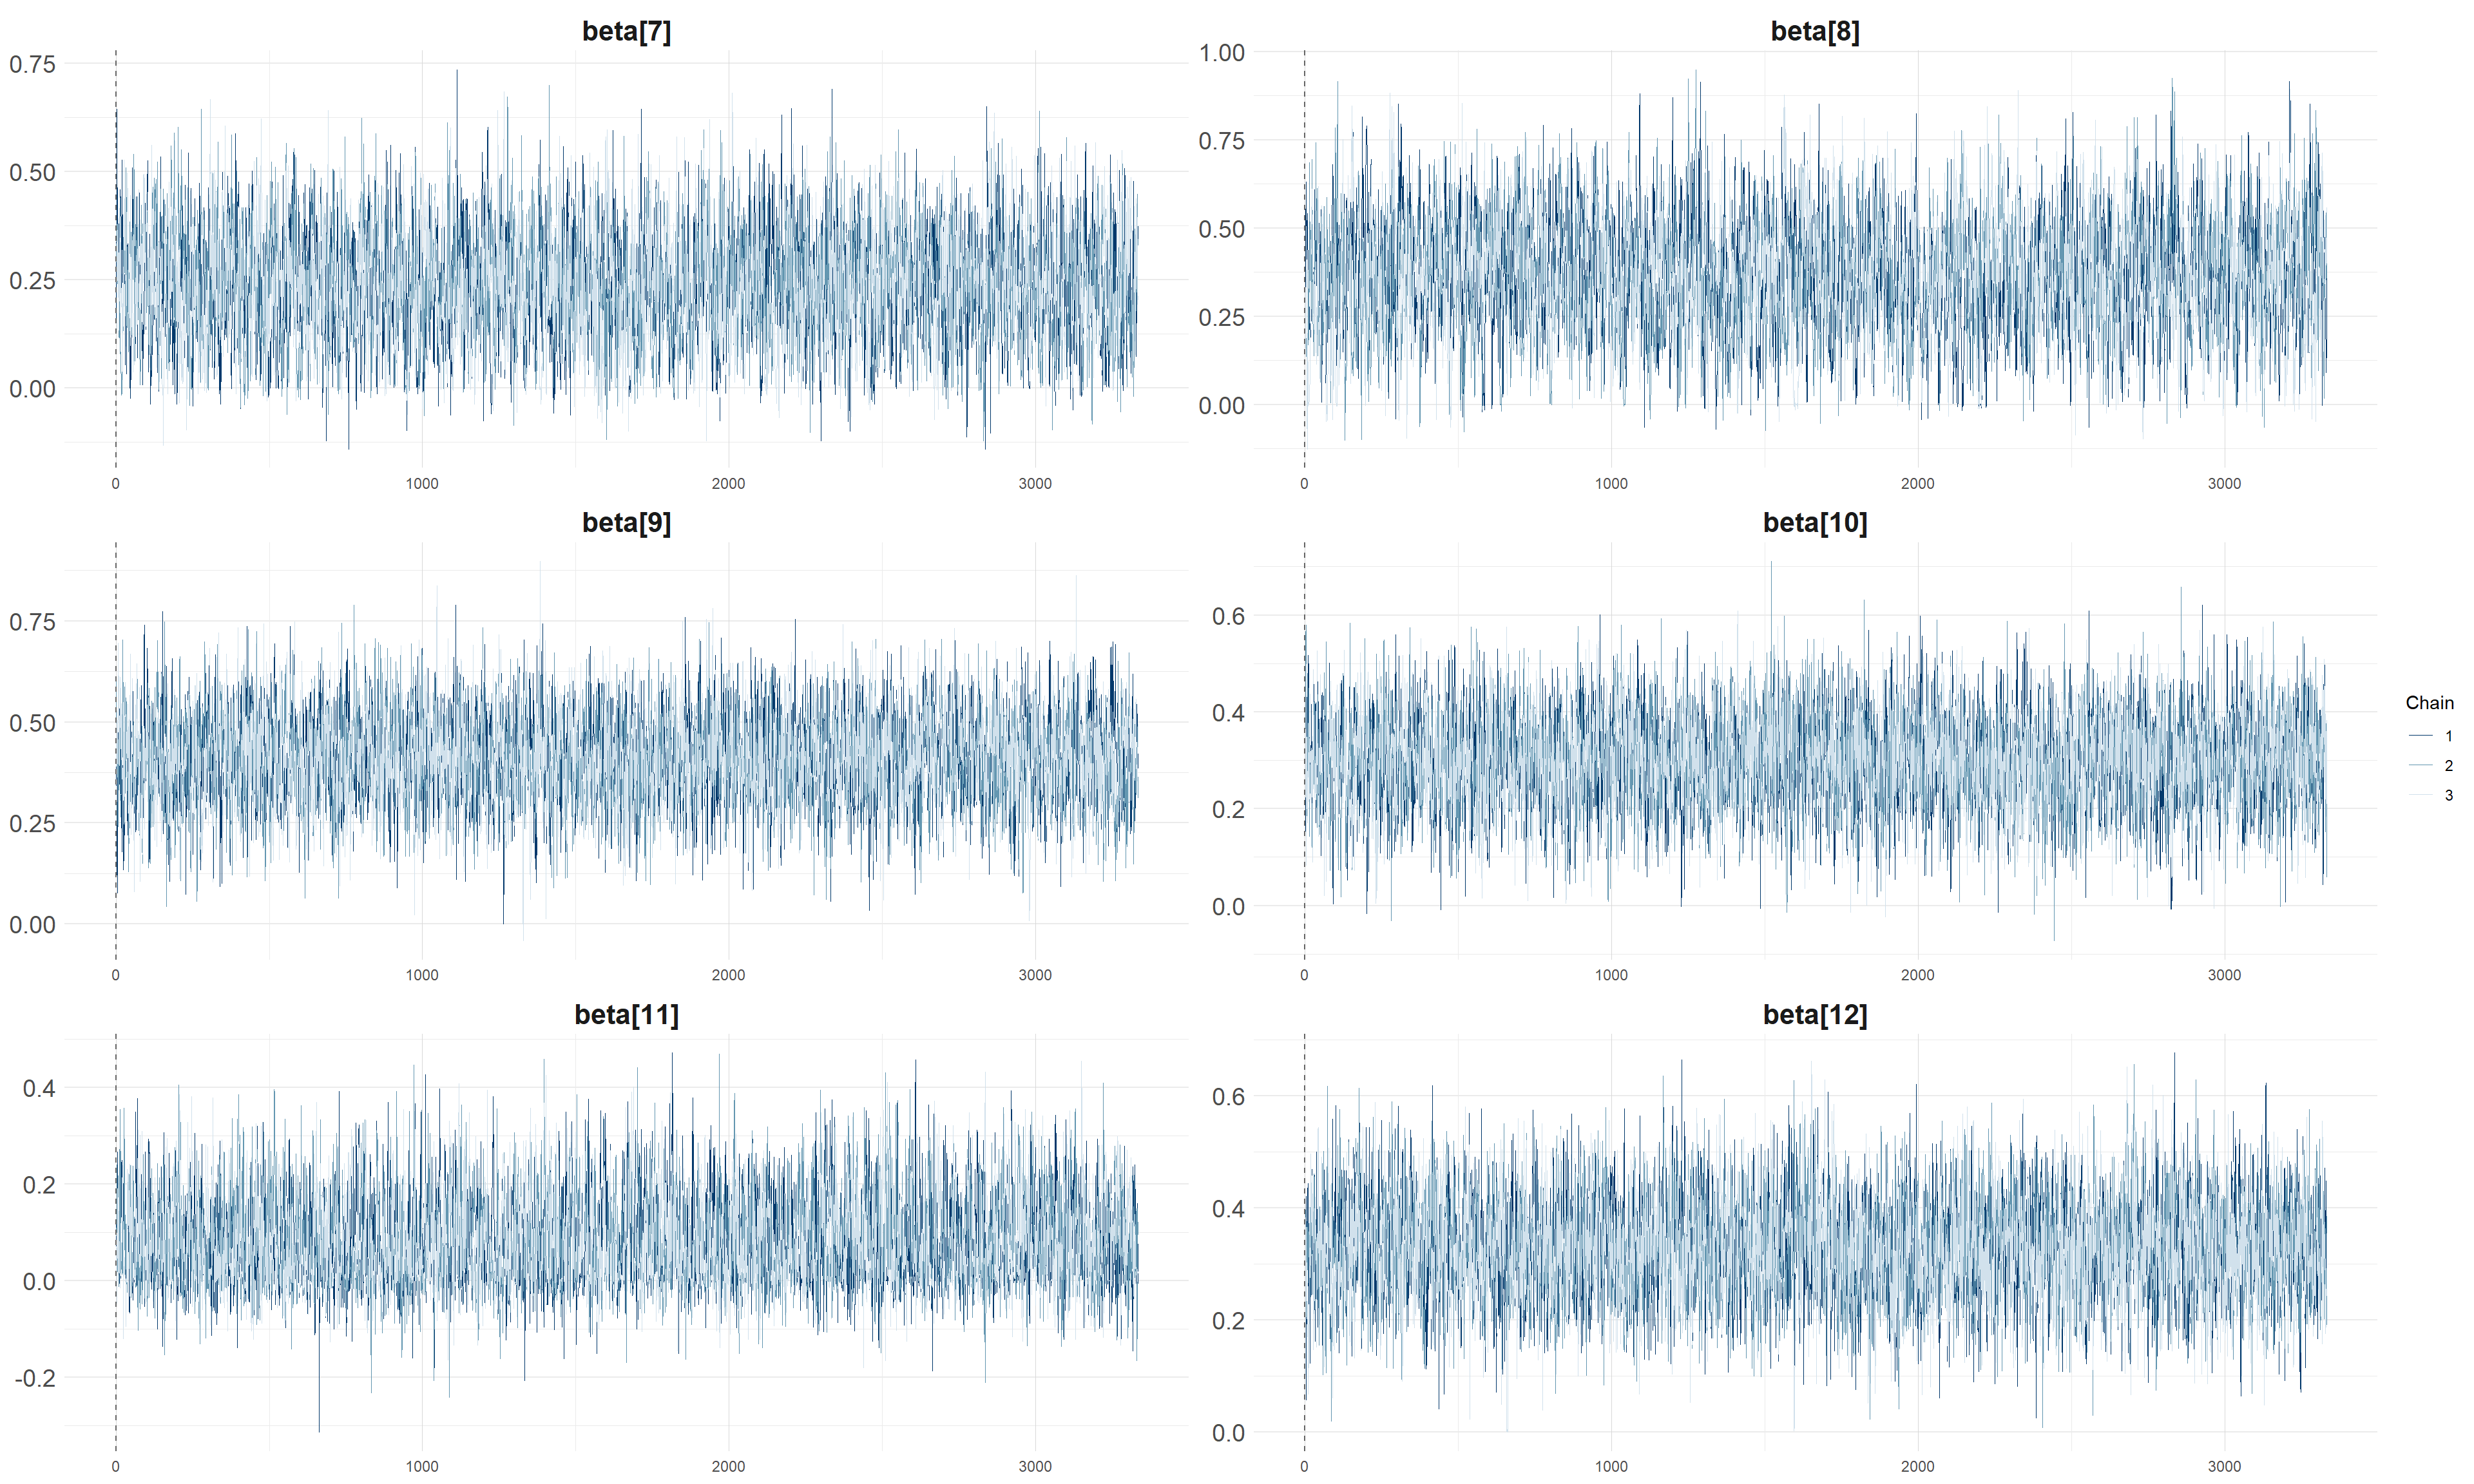
\includegraphics[width=\linewidth]{img/horseshoe_model/trace_beta_2.png}
    \caption{Group 2.}
  \end{subfigure}\hfill
  \begin{subfigure}[t]{0.48\linewidth}
    \centering
    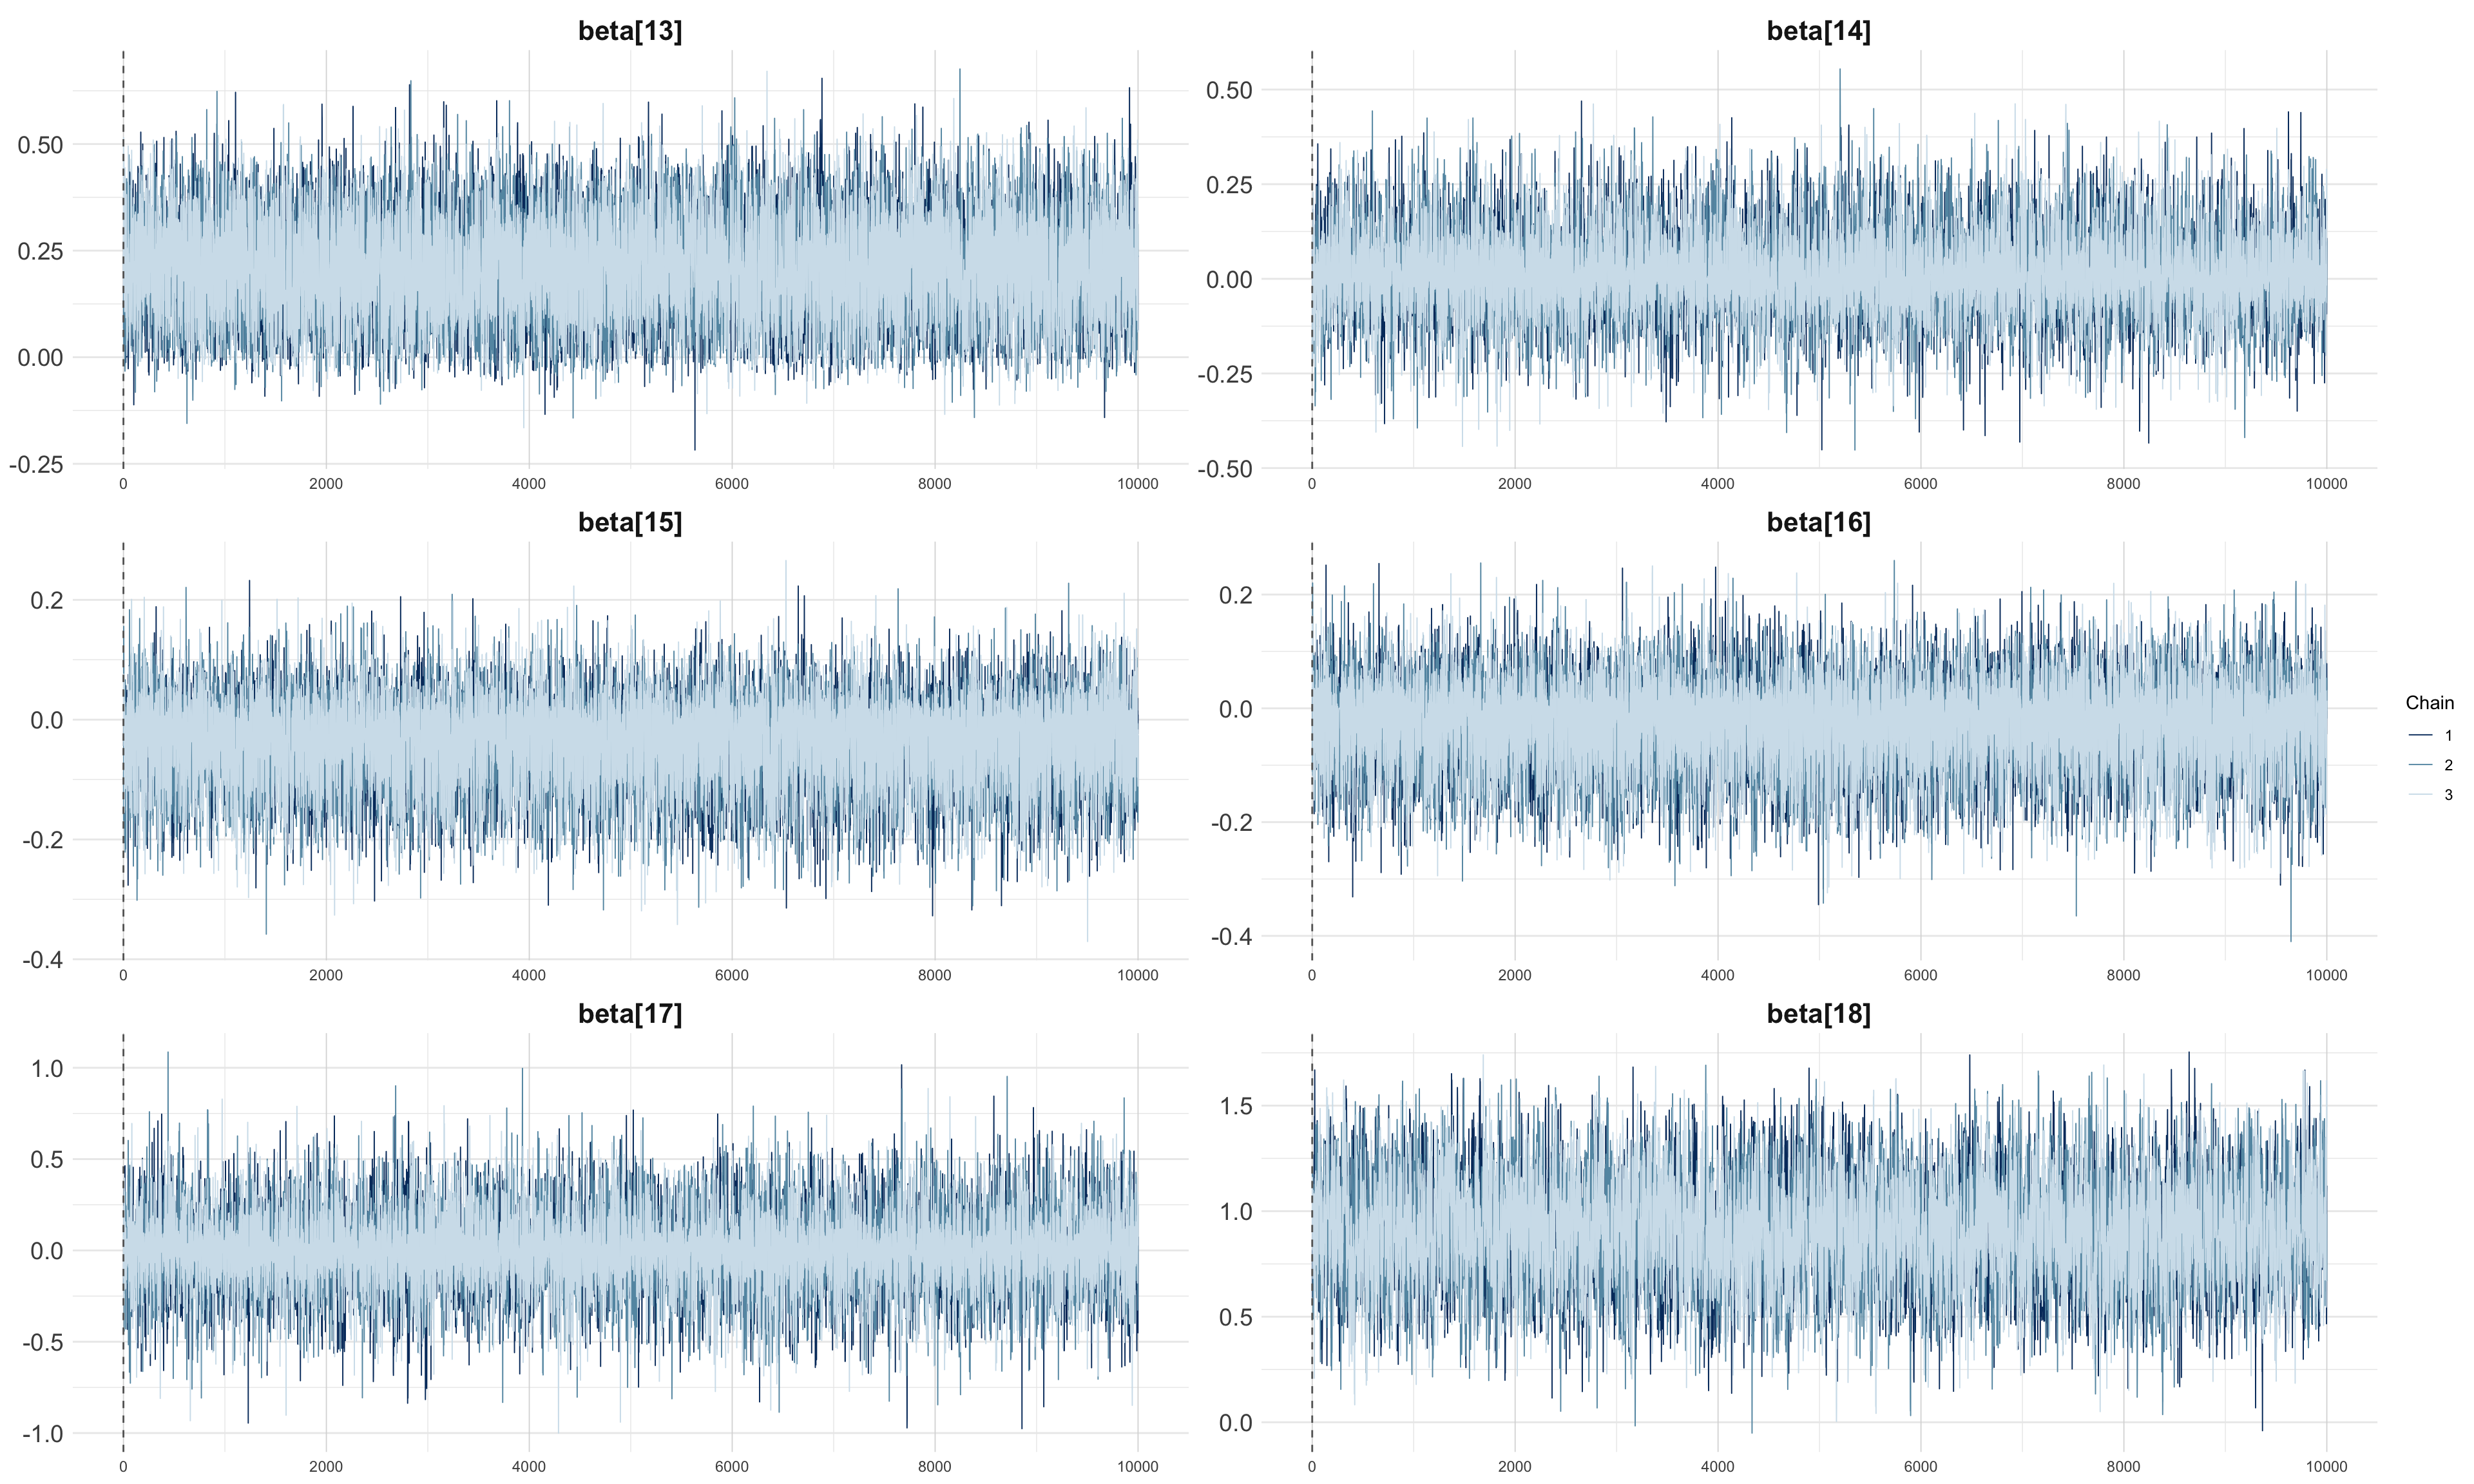
\includegraphics[width=\linewidth]{img/horseshoe_model/trace_beta_3.png}
    \caption{Group 3.}
  \end{subfigure}\hfill
  \begin{subfigure}[t]{0.48\linewidth}
    \centering
    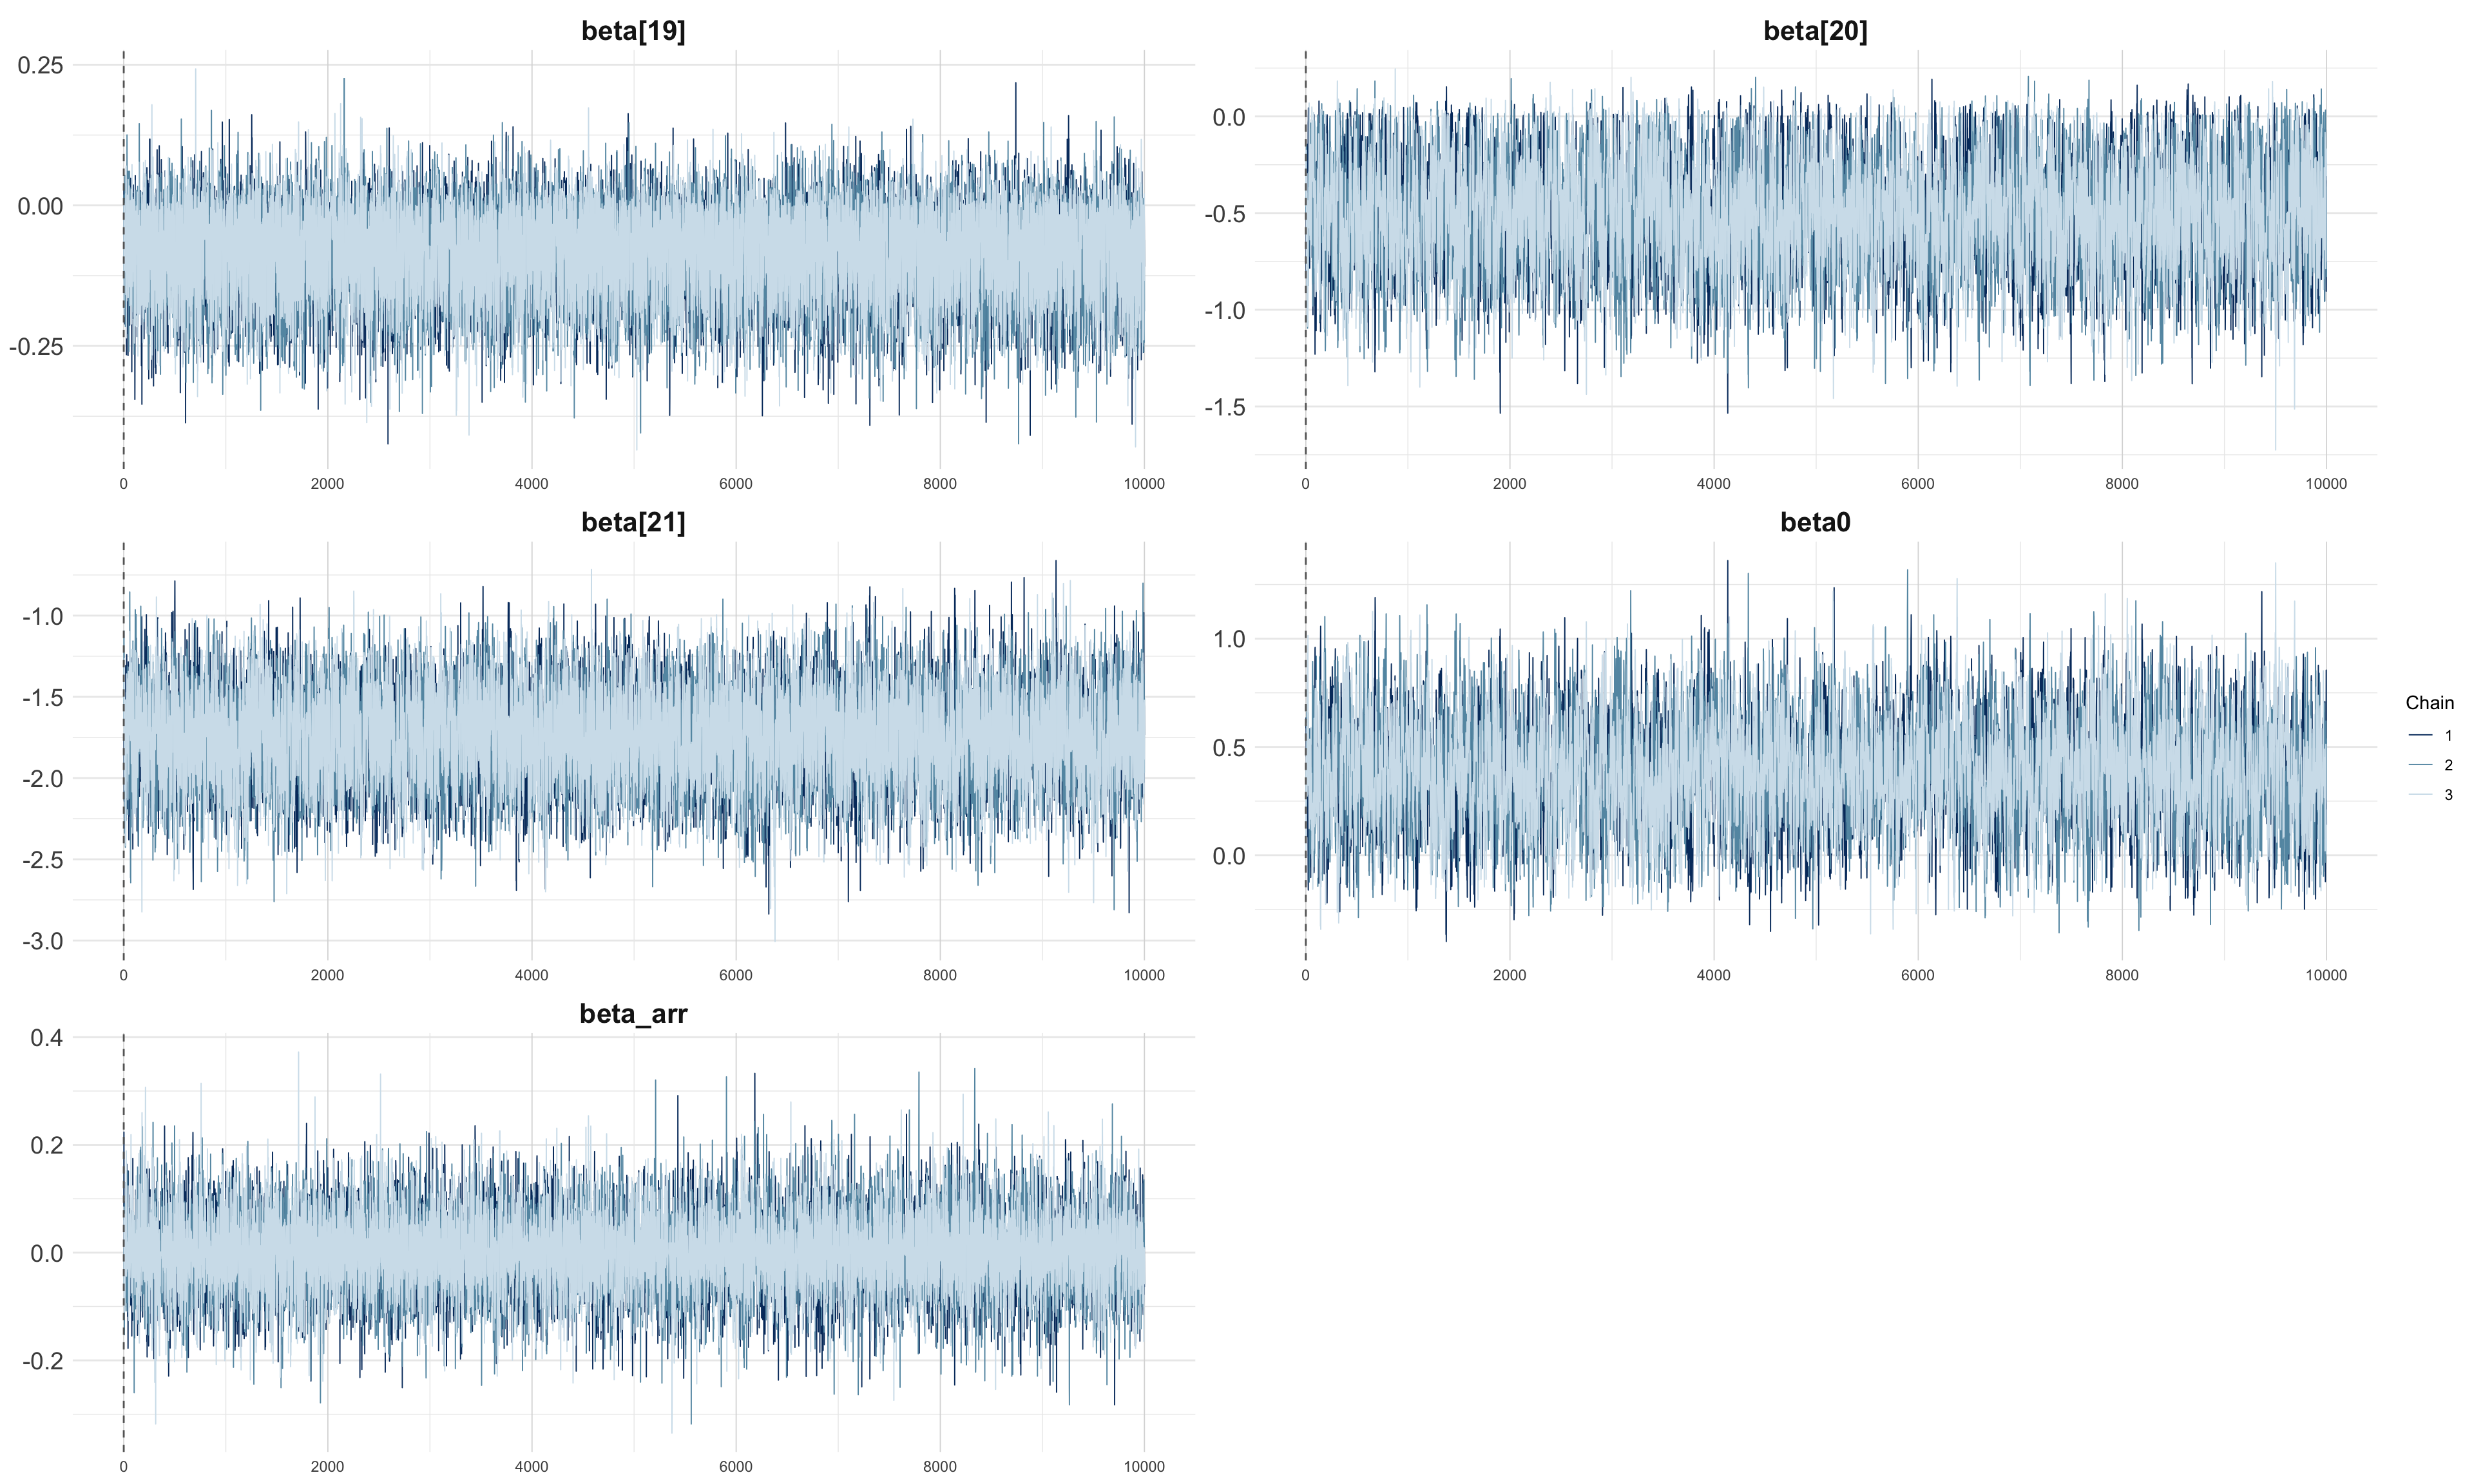
\includegraphics[width=\linewidth]{img/horseshoe_model/trace_beta_4.png}
    \caption{Group 4.}
  \end{subfigure}\hfill
  \caption{Trace plots for the remaining regression coefficients $\beta_j$, three chains.}
  \label{fig:hs_trace_beta_rest}
\end{figure}

\begin{figure}[htbp]
  \centering
  \begin{subfigure}[t]{0.48\linewidth}
    \centering
    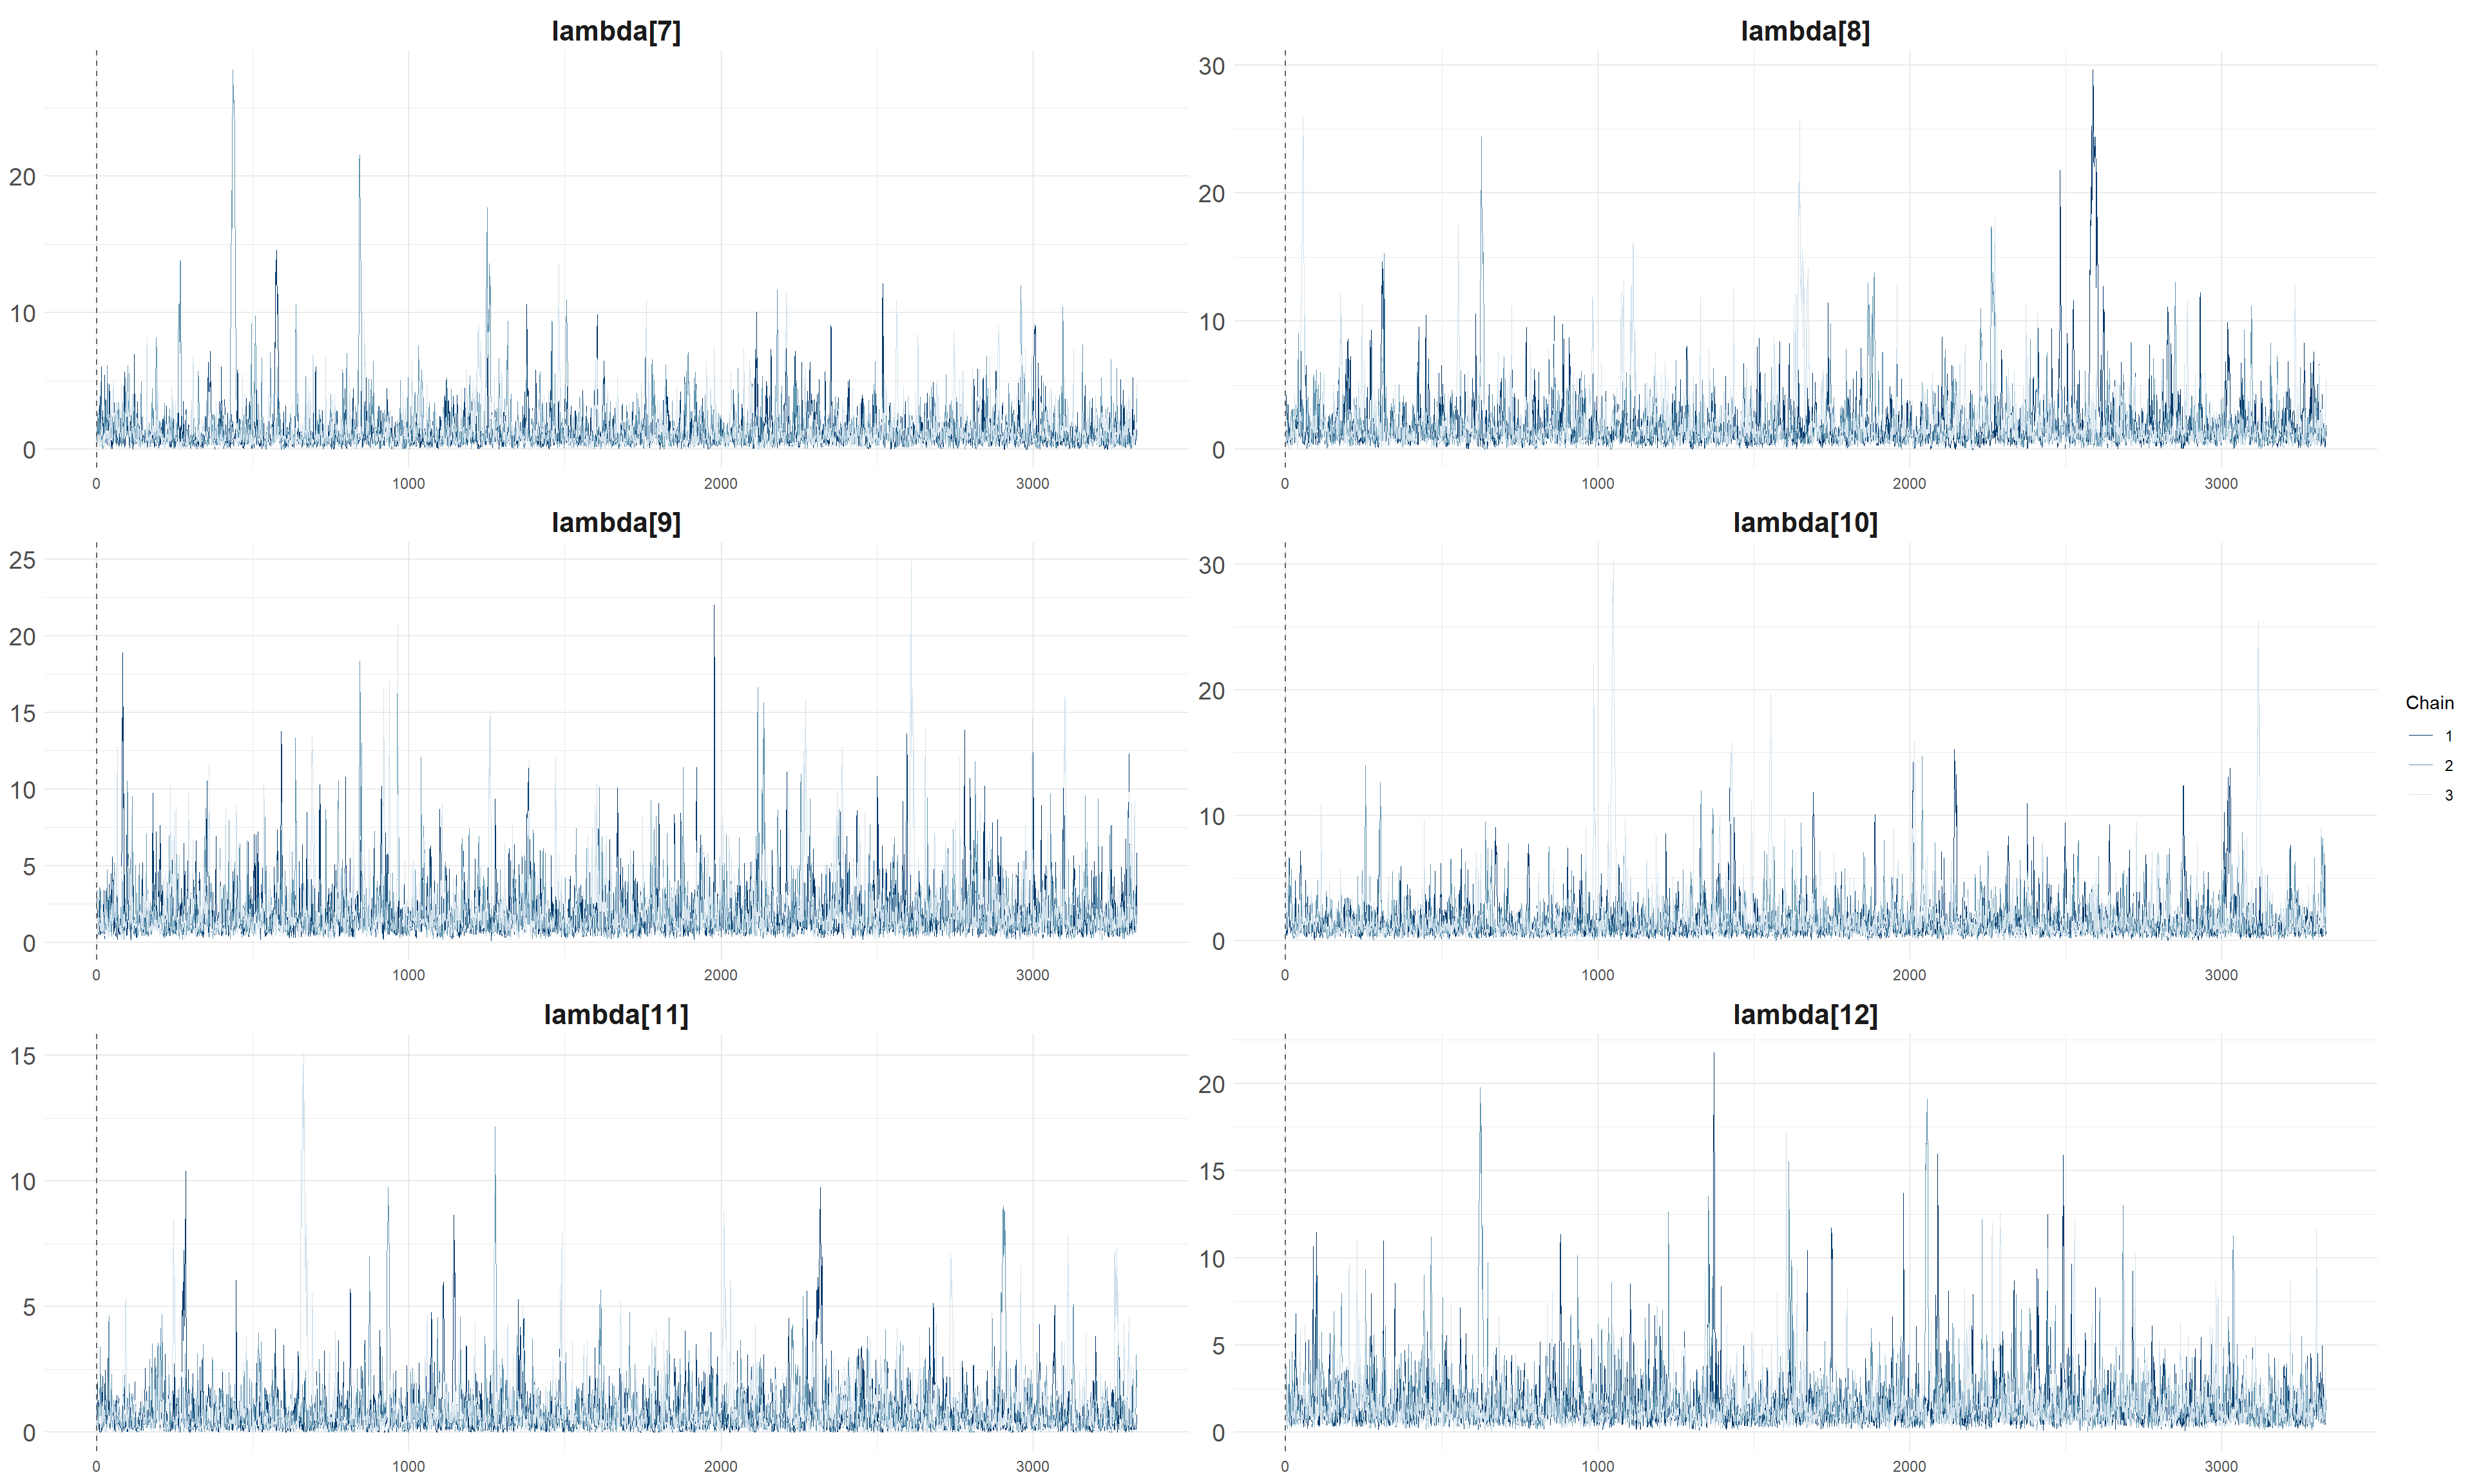
\includegraphics[width=\linewidth]{img/horseshoe_model/trace_lambda_2.png}
    \caption{Group 2.}
  \end{subfigure}\hfill
  \begin{subfigure}[t]{0.48\linewidth}
    \centering
    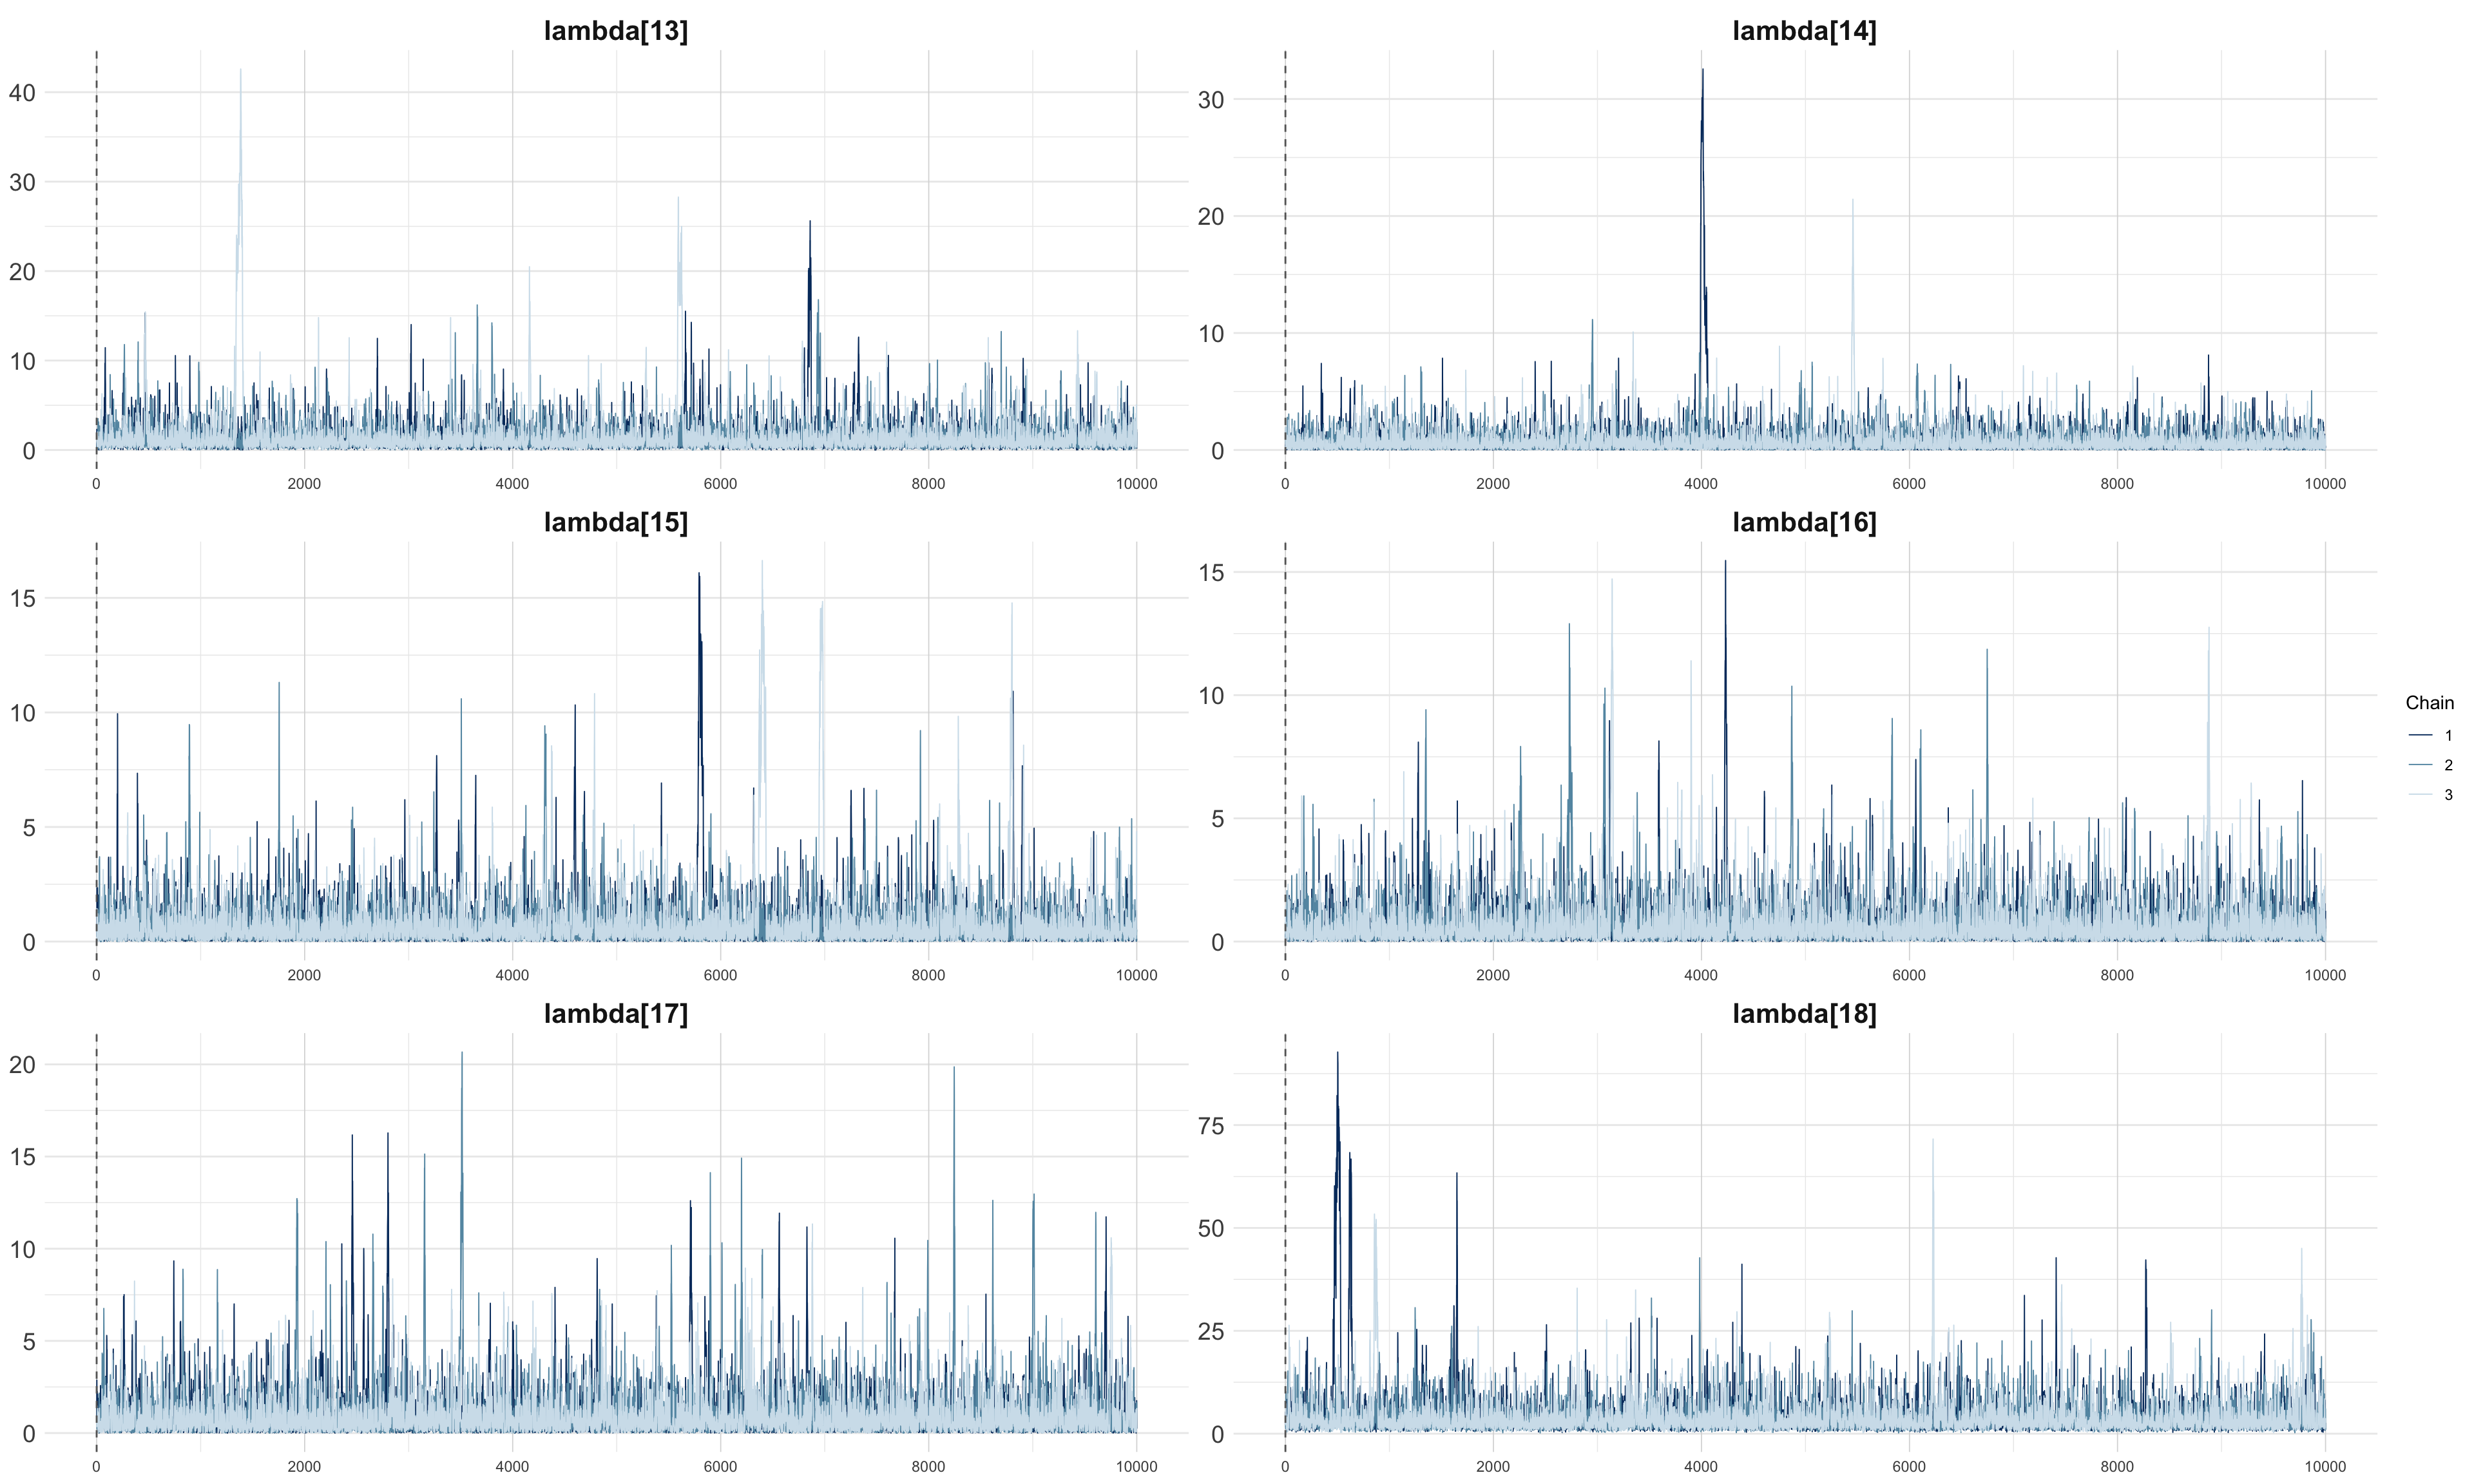
\includegraphics[width=\linewidth]{img/horseshoe_model/trace_lambda_3.png}
    \caption{Group 3.}
  \end{subfigure}\hfill
  \begin{subfigure}[t]{0.48\linewidth}
    \centering
    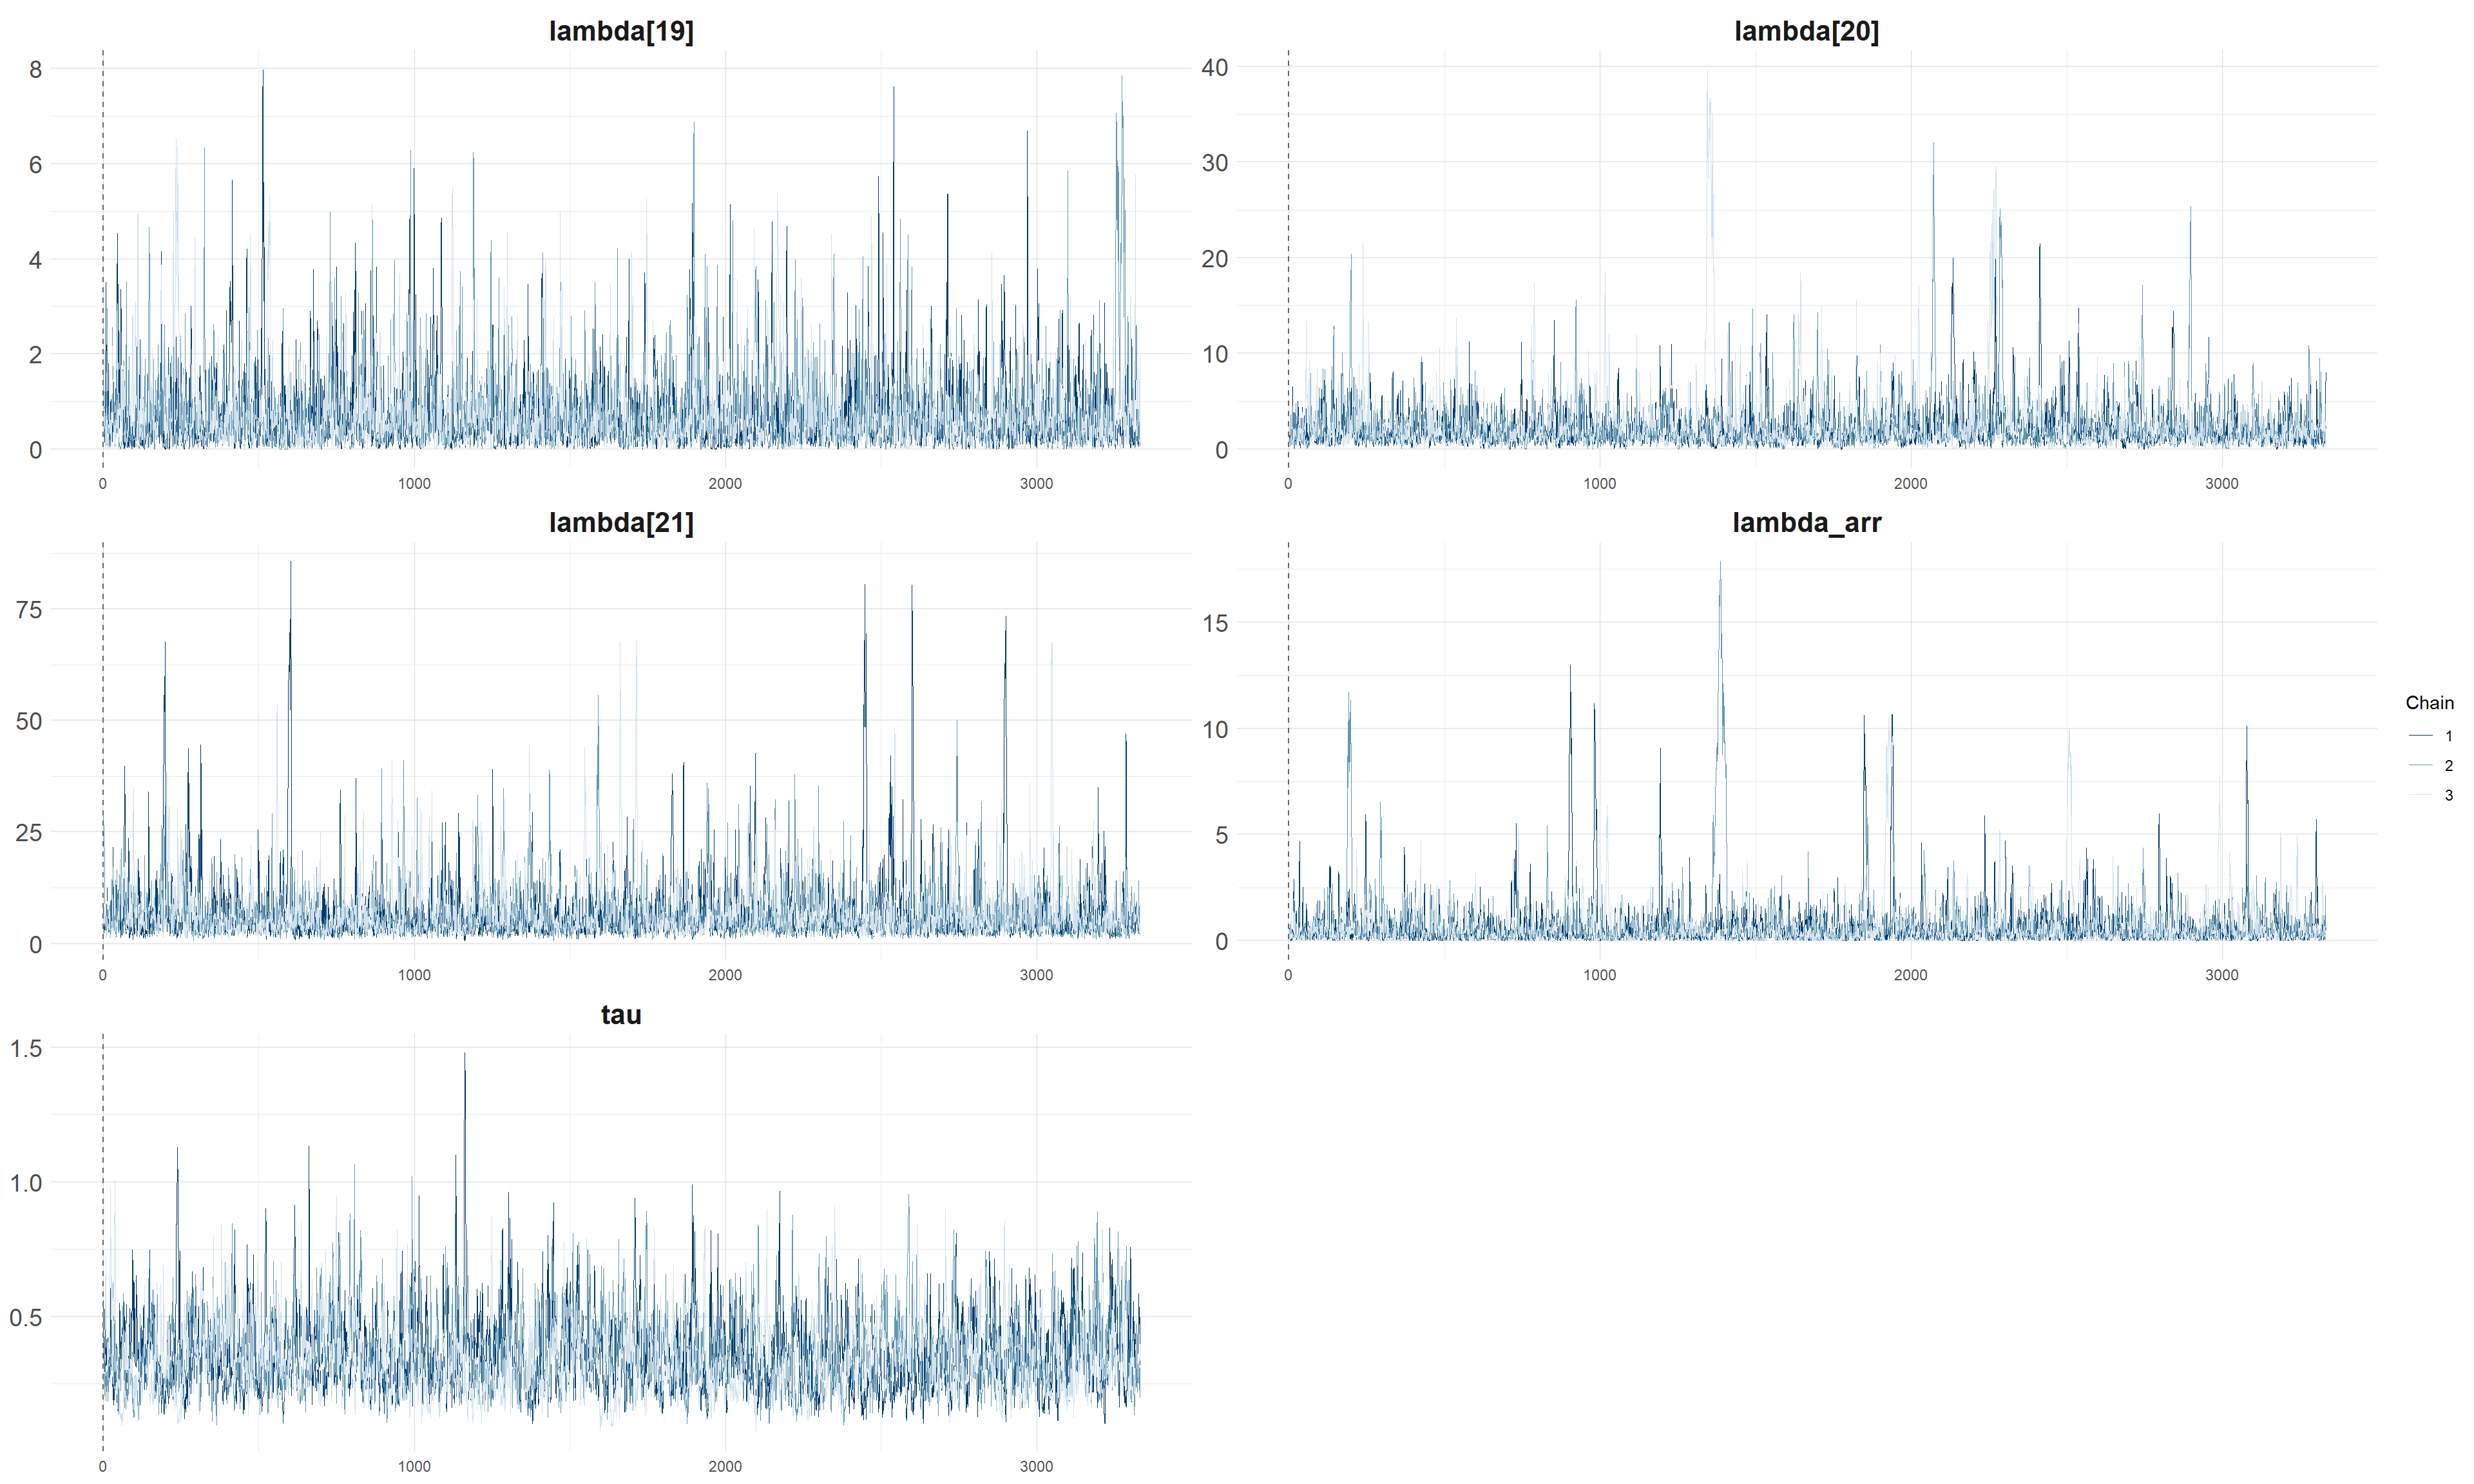
\includegraphics[width=\linewidth]{img/horseshoe_model/trace_lambda_4.png}
    \caption{Group 4.}
  \end{subfigure}\hfill
  \caption{Trace plots for the remaining scale parameters $\lambda_j$, three chains.}
  \label{fig:hs_trace_lambda_rest}
\end{figure}

\subsection*{Autocorrelation}
Autocorrelation functions for every parameter, one set per chain. The
coefficients decay within a few lags; the local scales decay more slowly, which
is the expected behaviour for a horseshoe and the reason for the thinning.
\begin{figure}[htbp]
  \centering
  \begin{subfigure}[t]{0.48\linewidth}
    \centering
    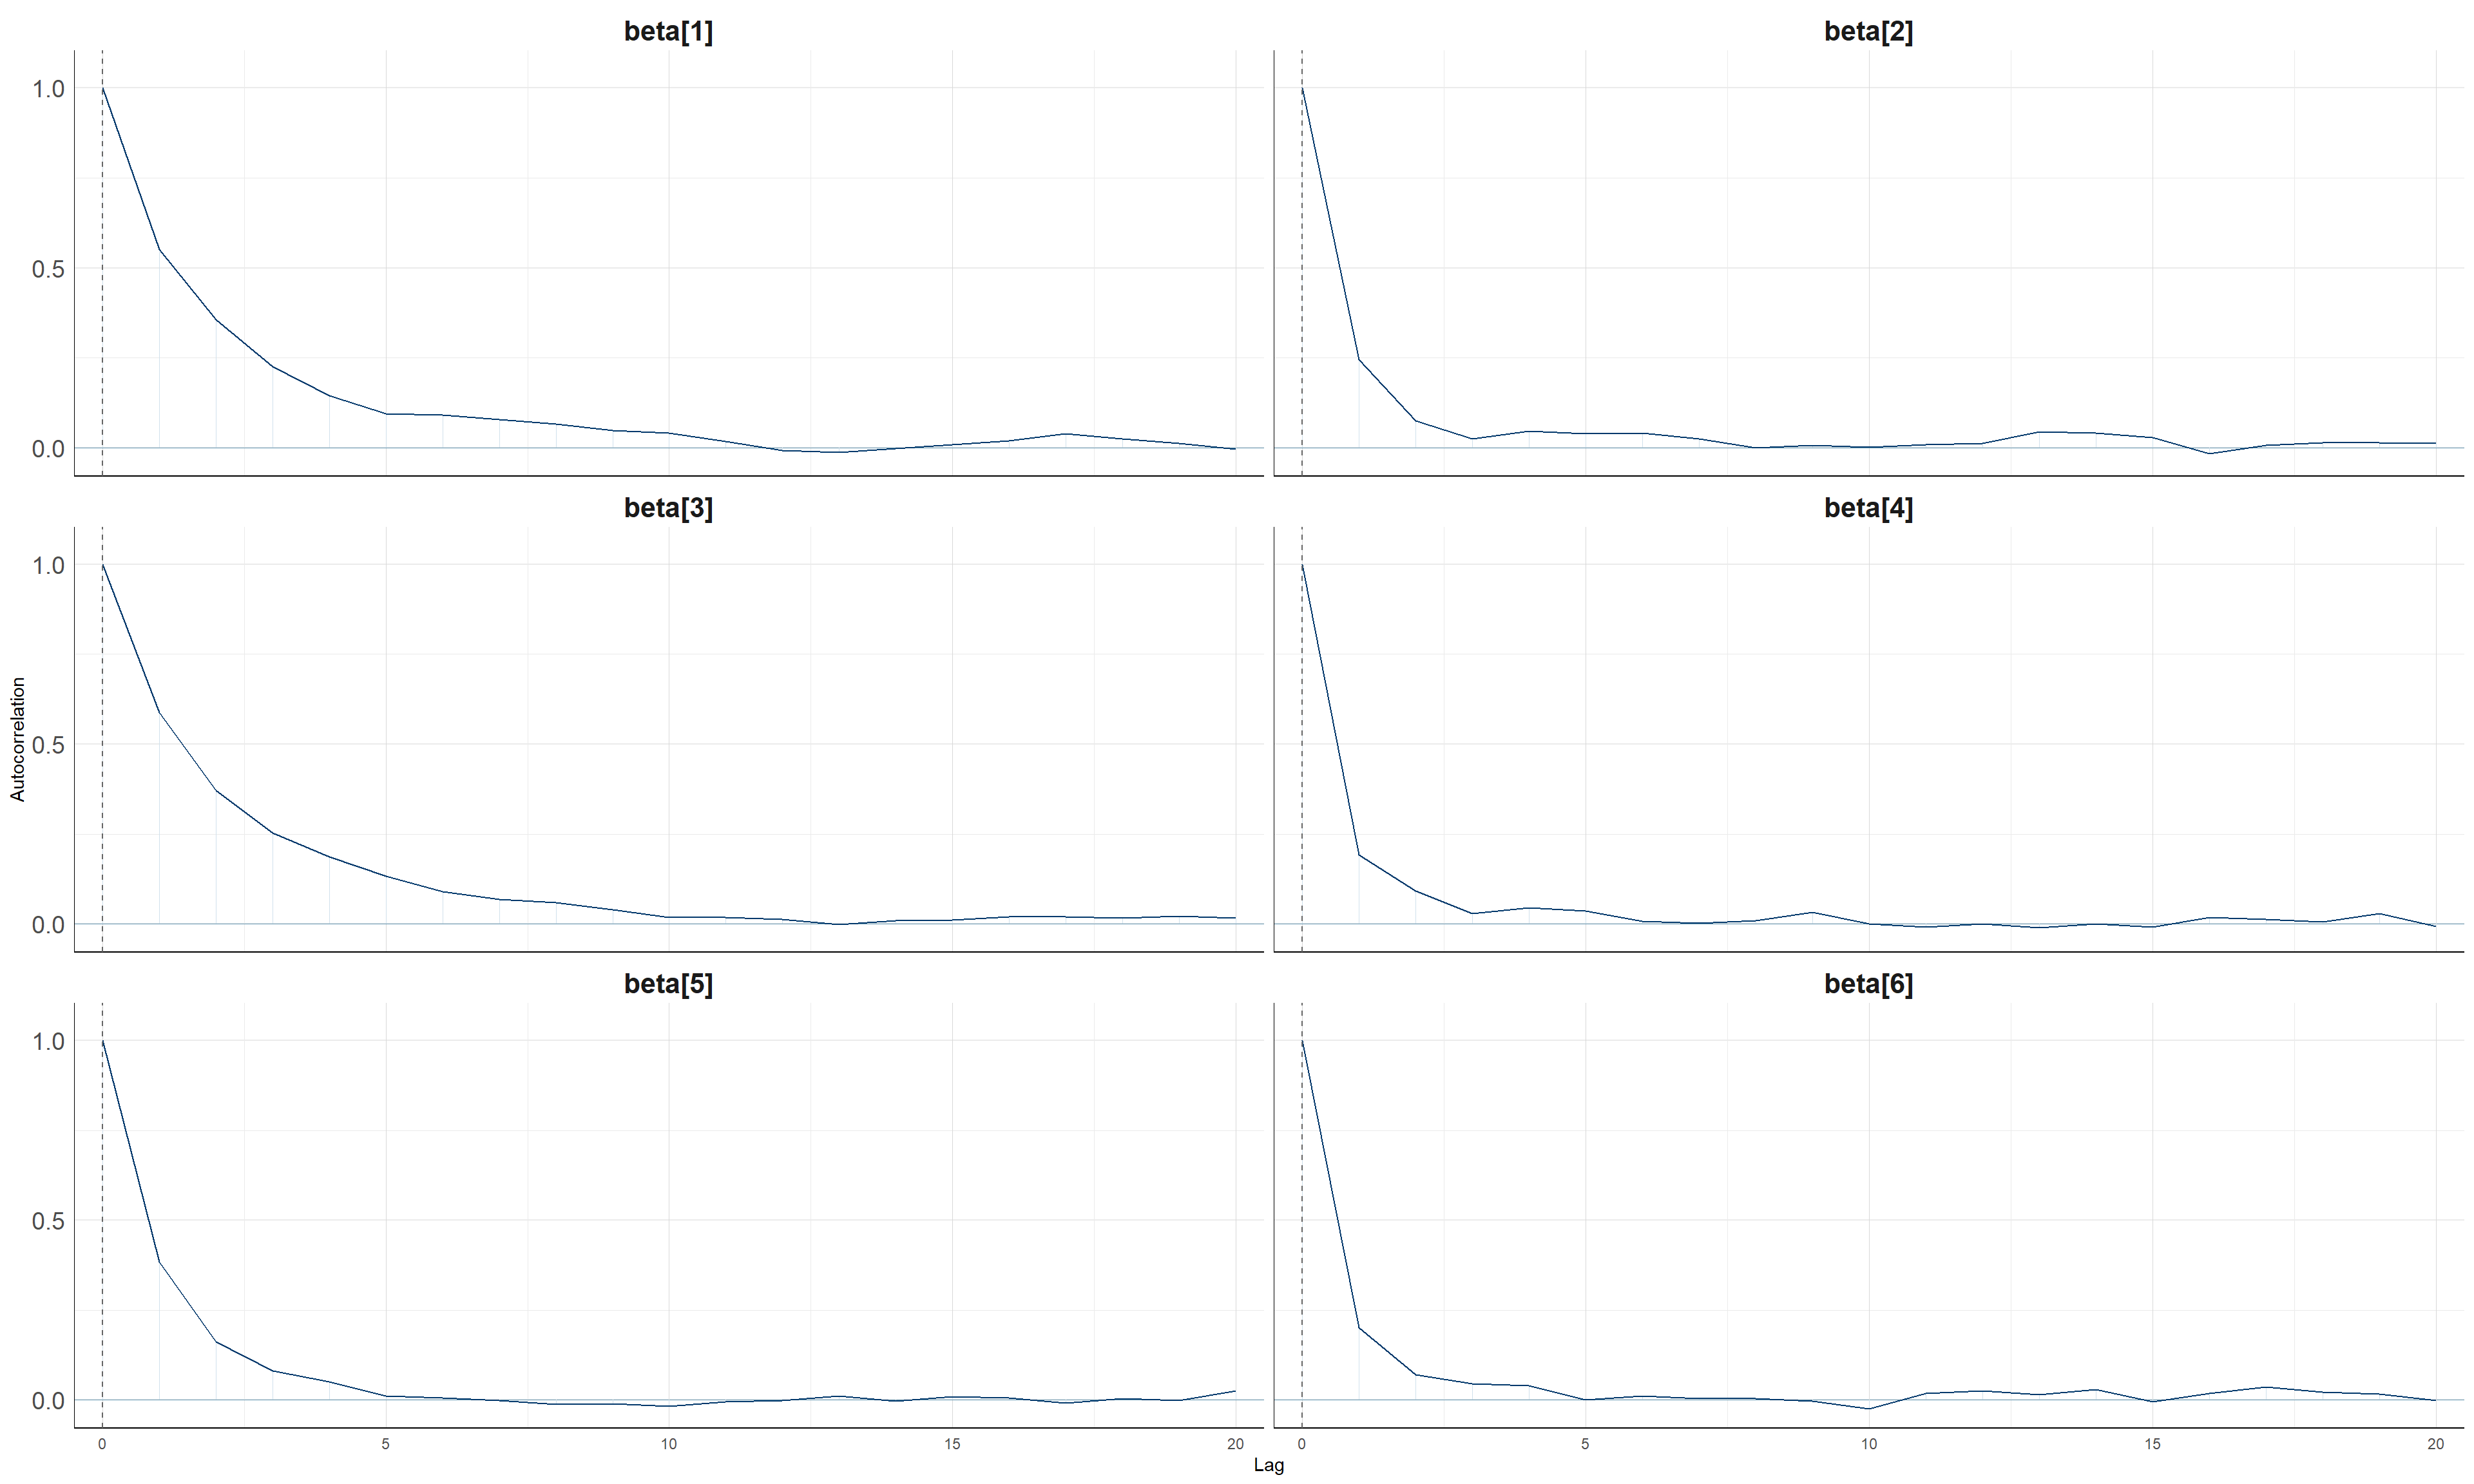
\includegraphics[width=\linewidth]{img/horseshoe_model/acf_beta_chain1_1.png}
    \caption{Group 1.}
  \end{subfigure}\hfill
  \begin{subfigure}[t]{0.48\linewidth}
    \centering
    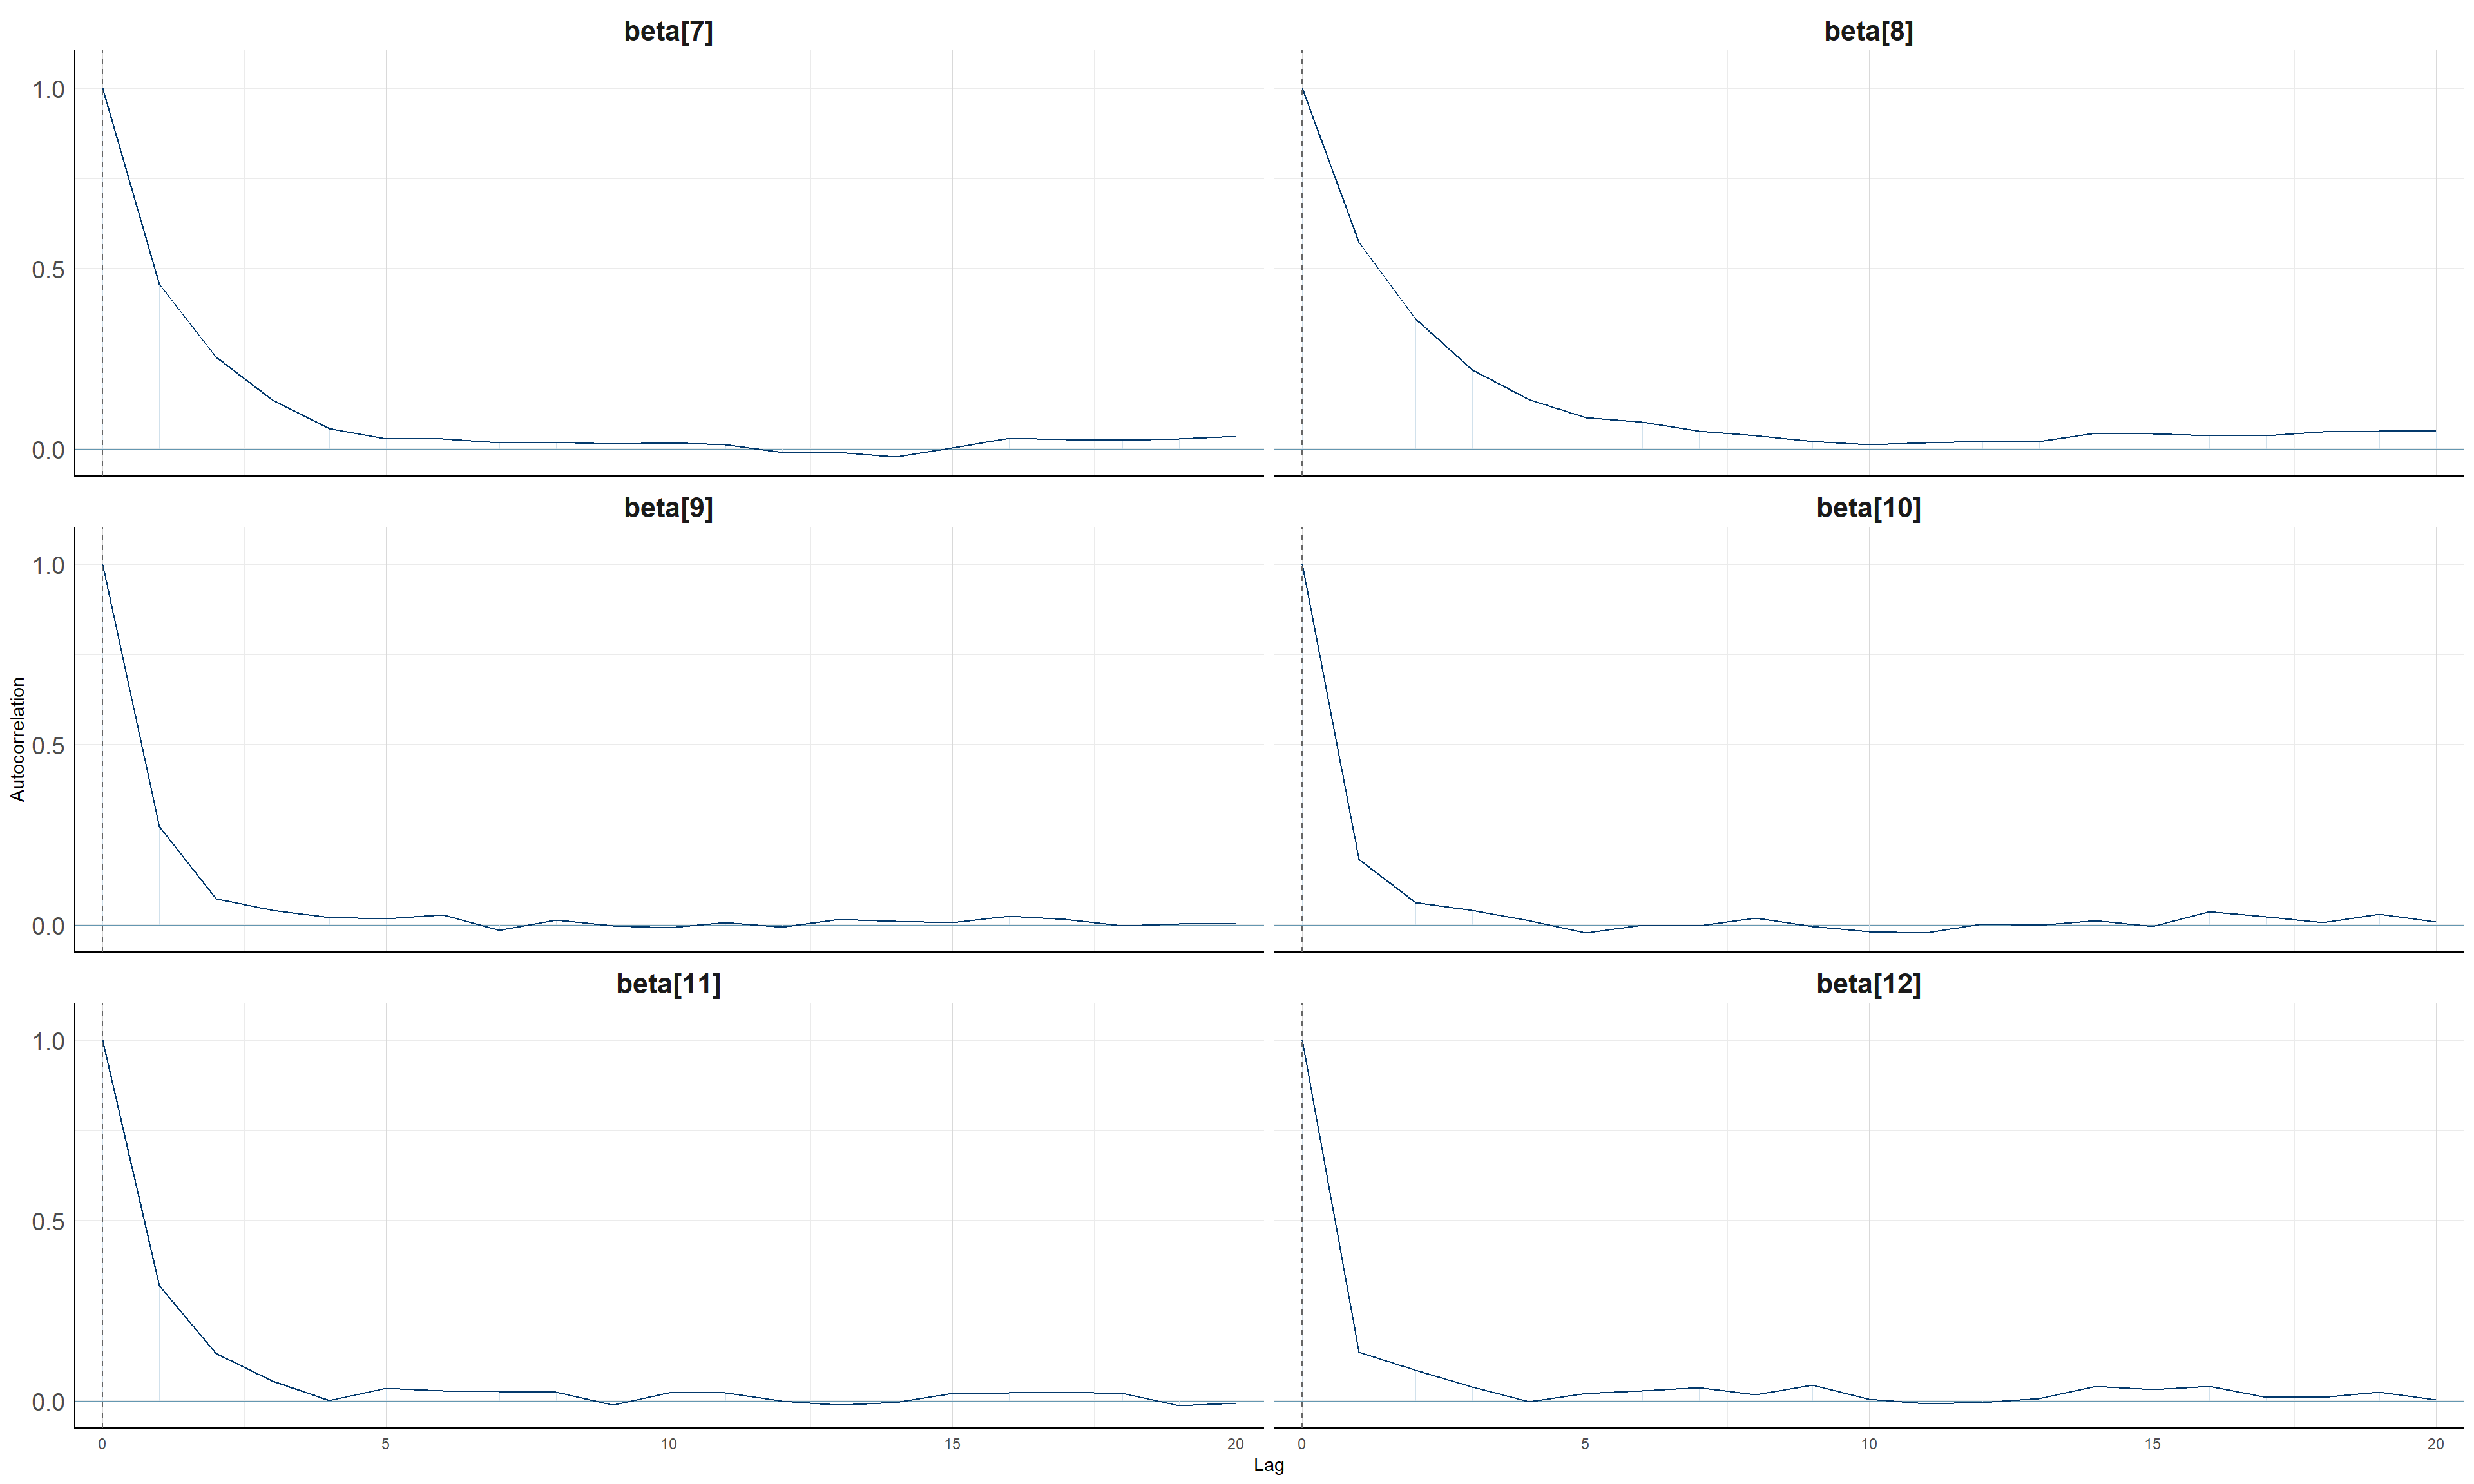
\includegraphics[width=\linewidth]{img/horseshoe_model/acf_beta_chain1_2.png}
    \caption{Group 2.}
  \end{subfigure}\hfill
  \begin{subfigure}[t]{0.48\linewidth}
    \centering
    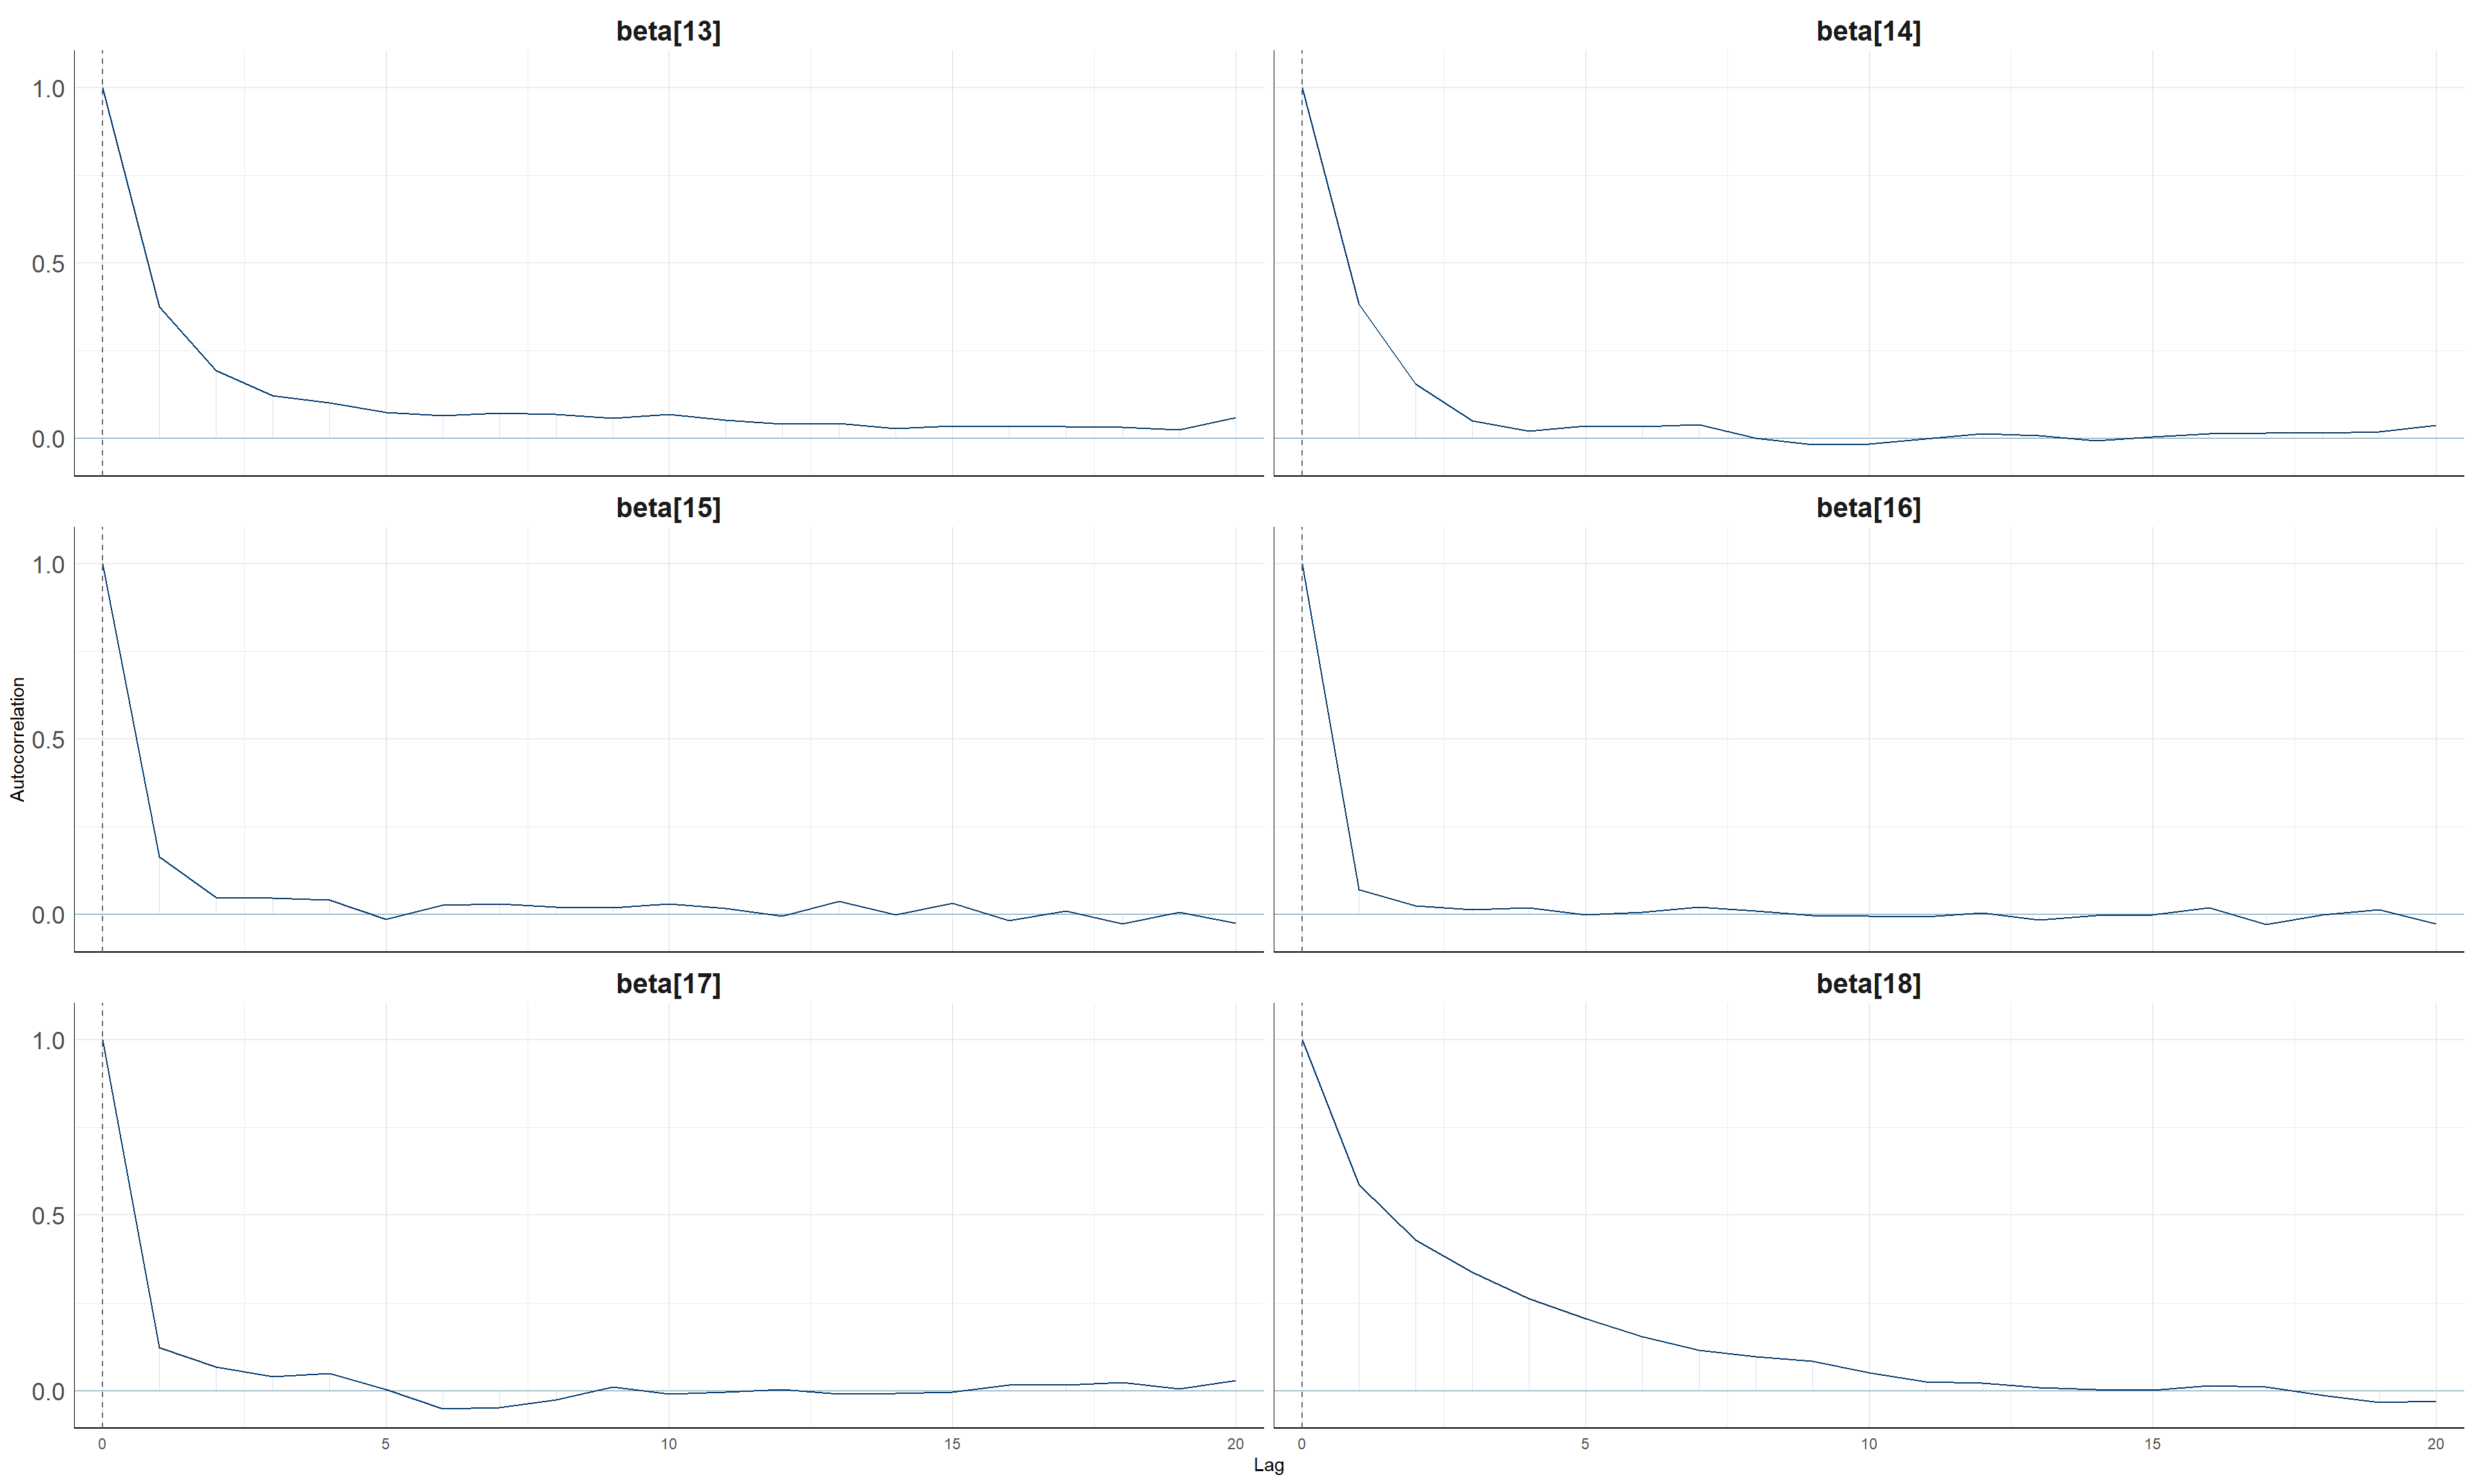
\includegraphics[width=\linewidth]{img/horseshoe_model/acf_beta_chain1_3.png}
    \caption{Group 3.}
  \end{subfigure}\hfill
  \begin{subfigure}[t]{0.48\linewidth}
    \centering
    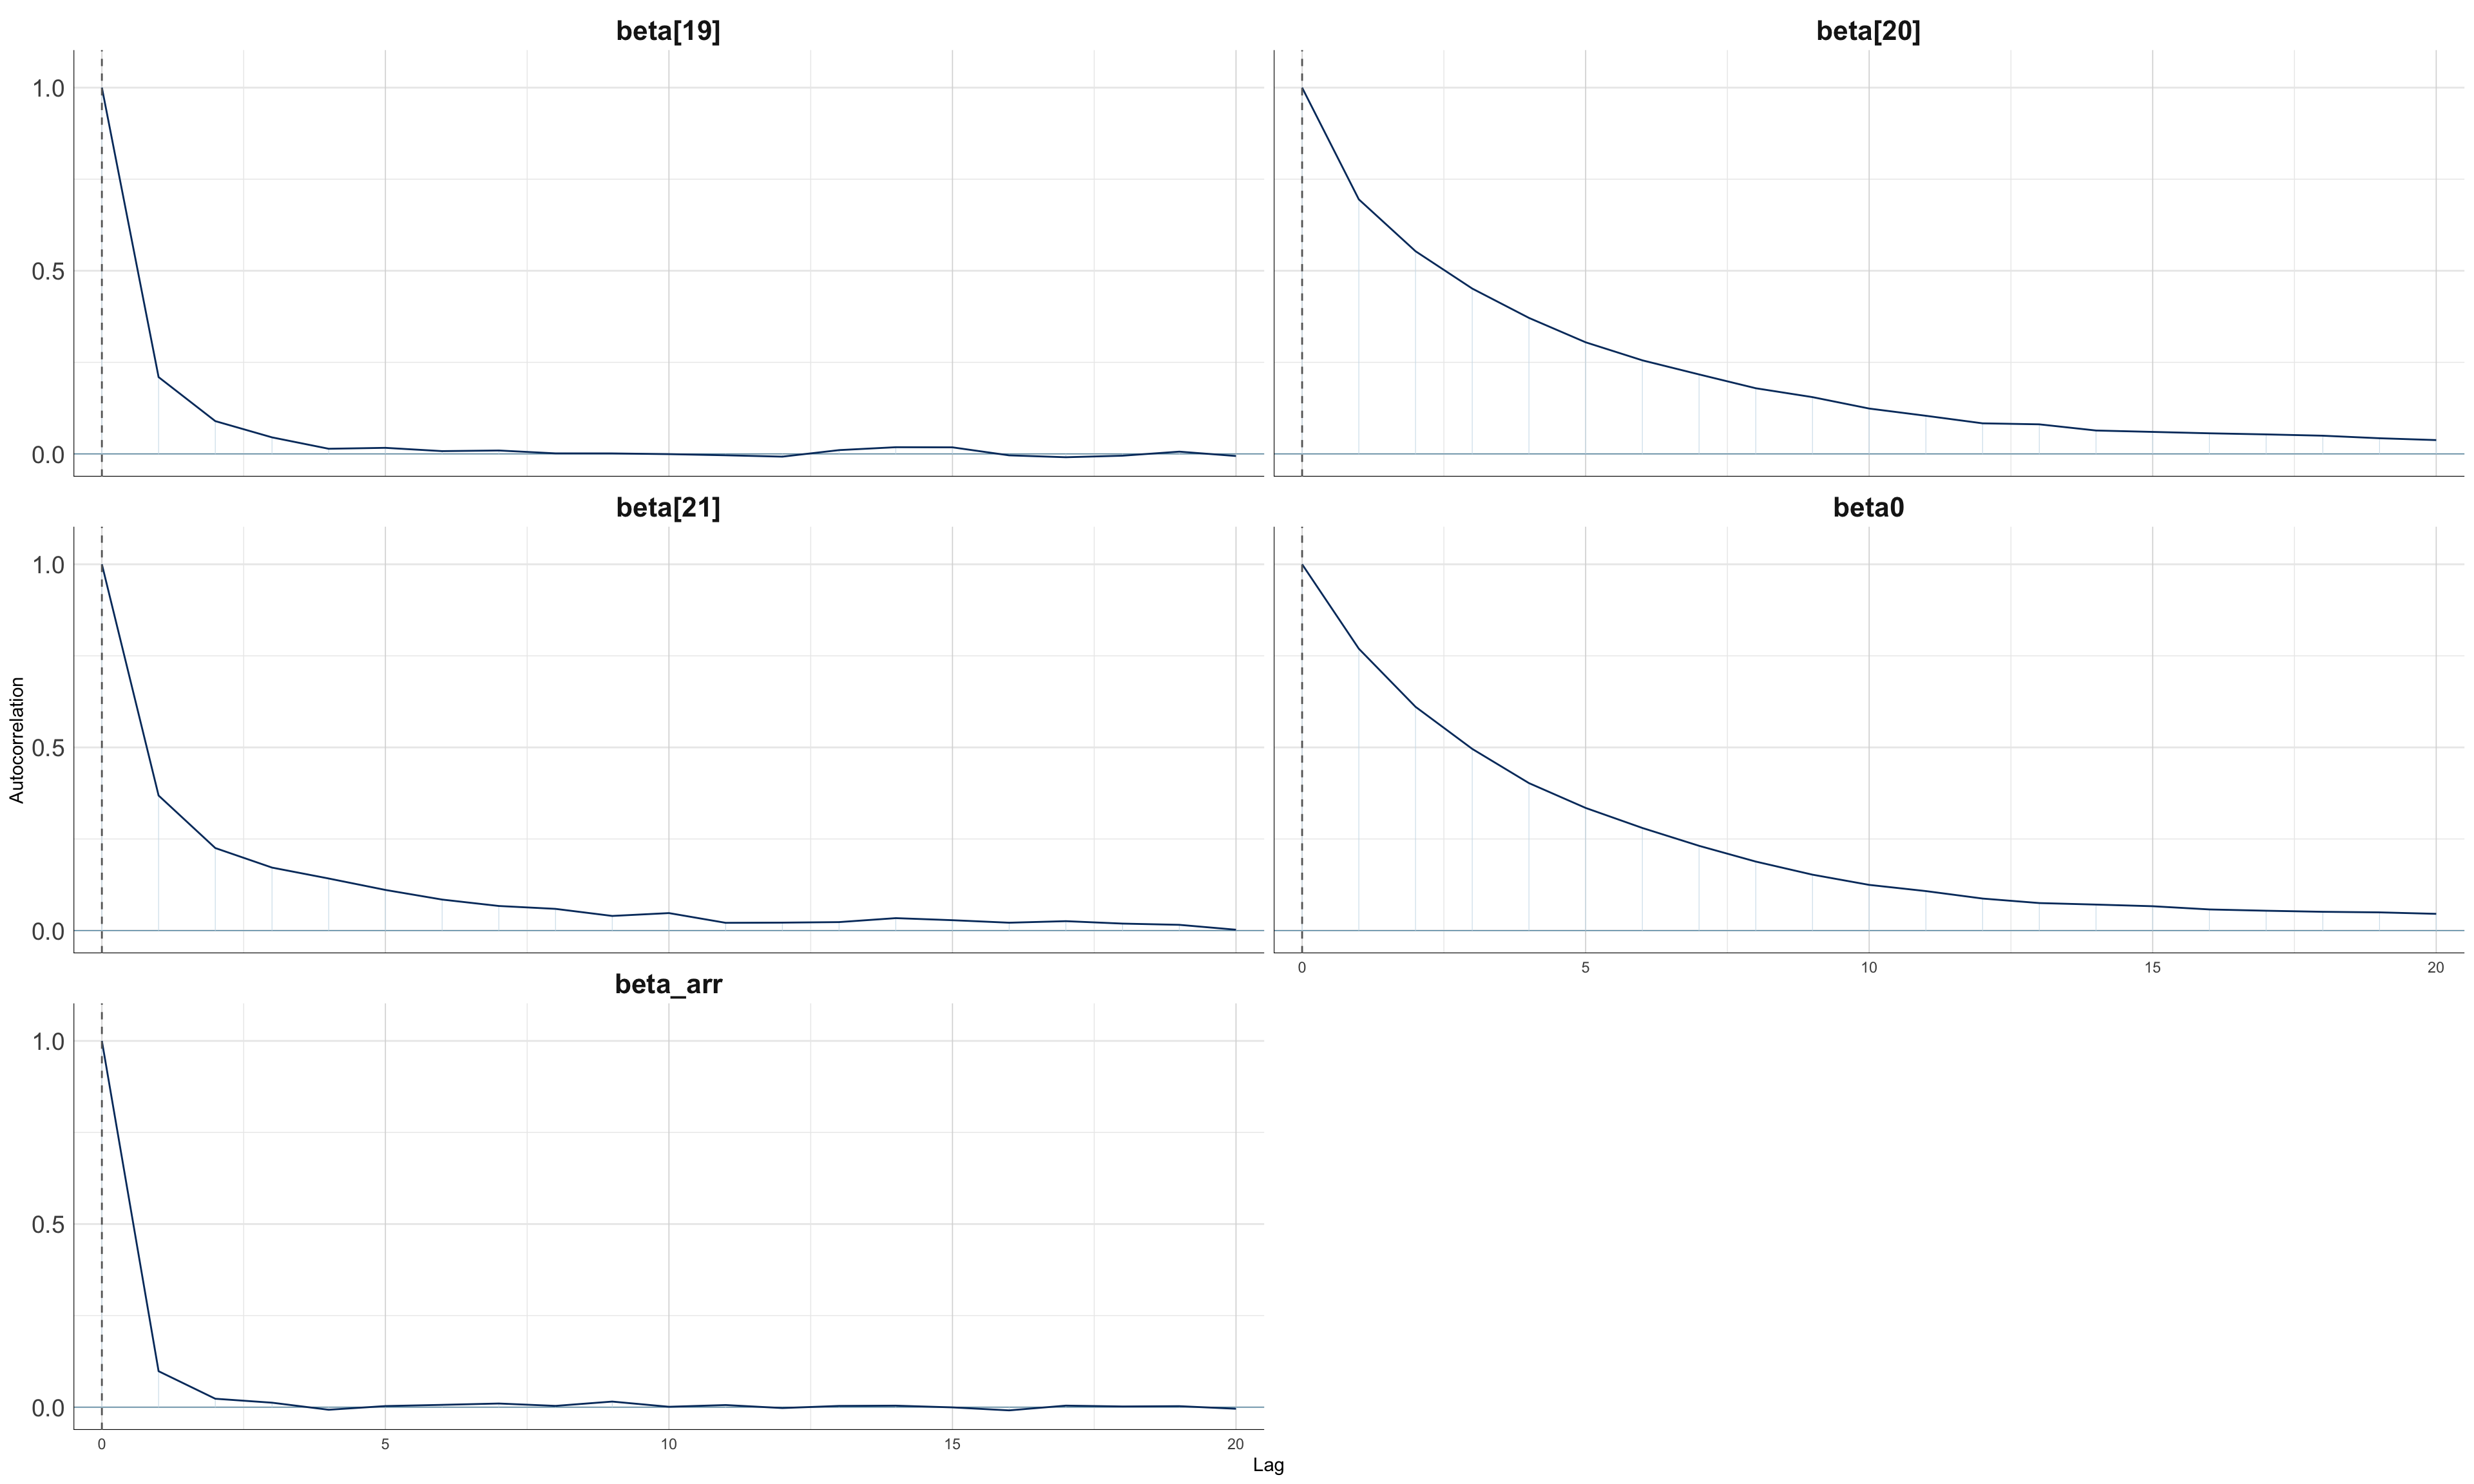
\includegraphics[width=\linewidth]{img/horseshoe_model/acf_beta_chain1_4.png}
    \caption{Group 4.}
  \end{subfigure}\hfill
  \caption{Autocorrelation of the coefficients $\beta_j$, chain 1.}
  \label{fig:hs_acf_beta_1}
\end{figure}

\begin{figure}[htbp]
  \centering
  \begin{subfigure}[t]{0.48\linewidth}
    \centering
    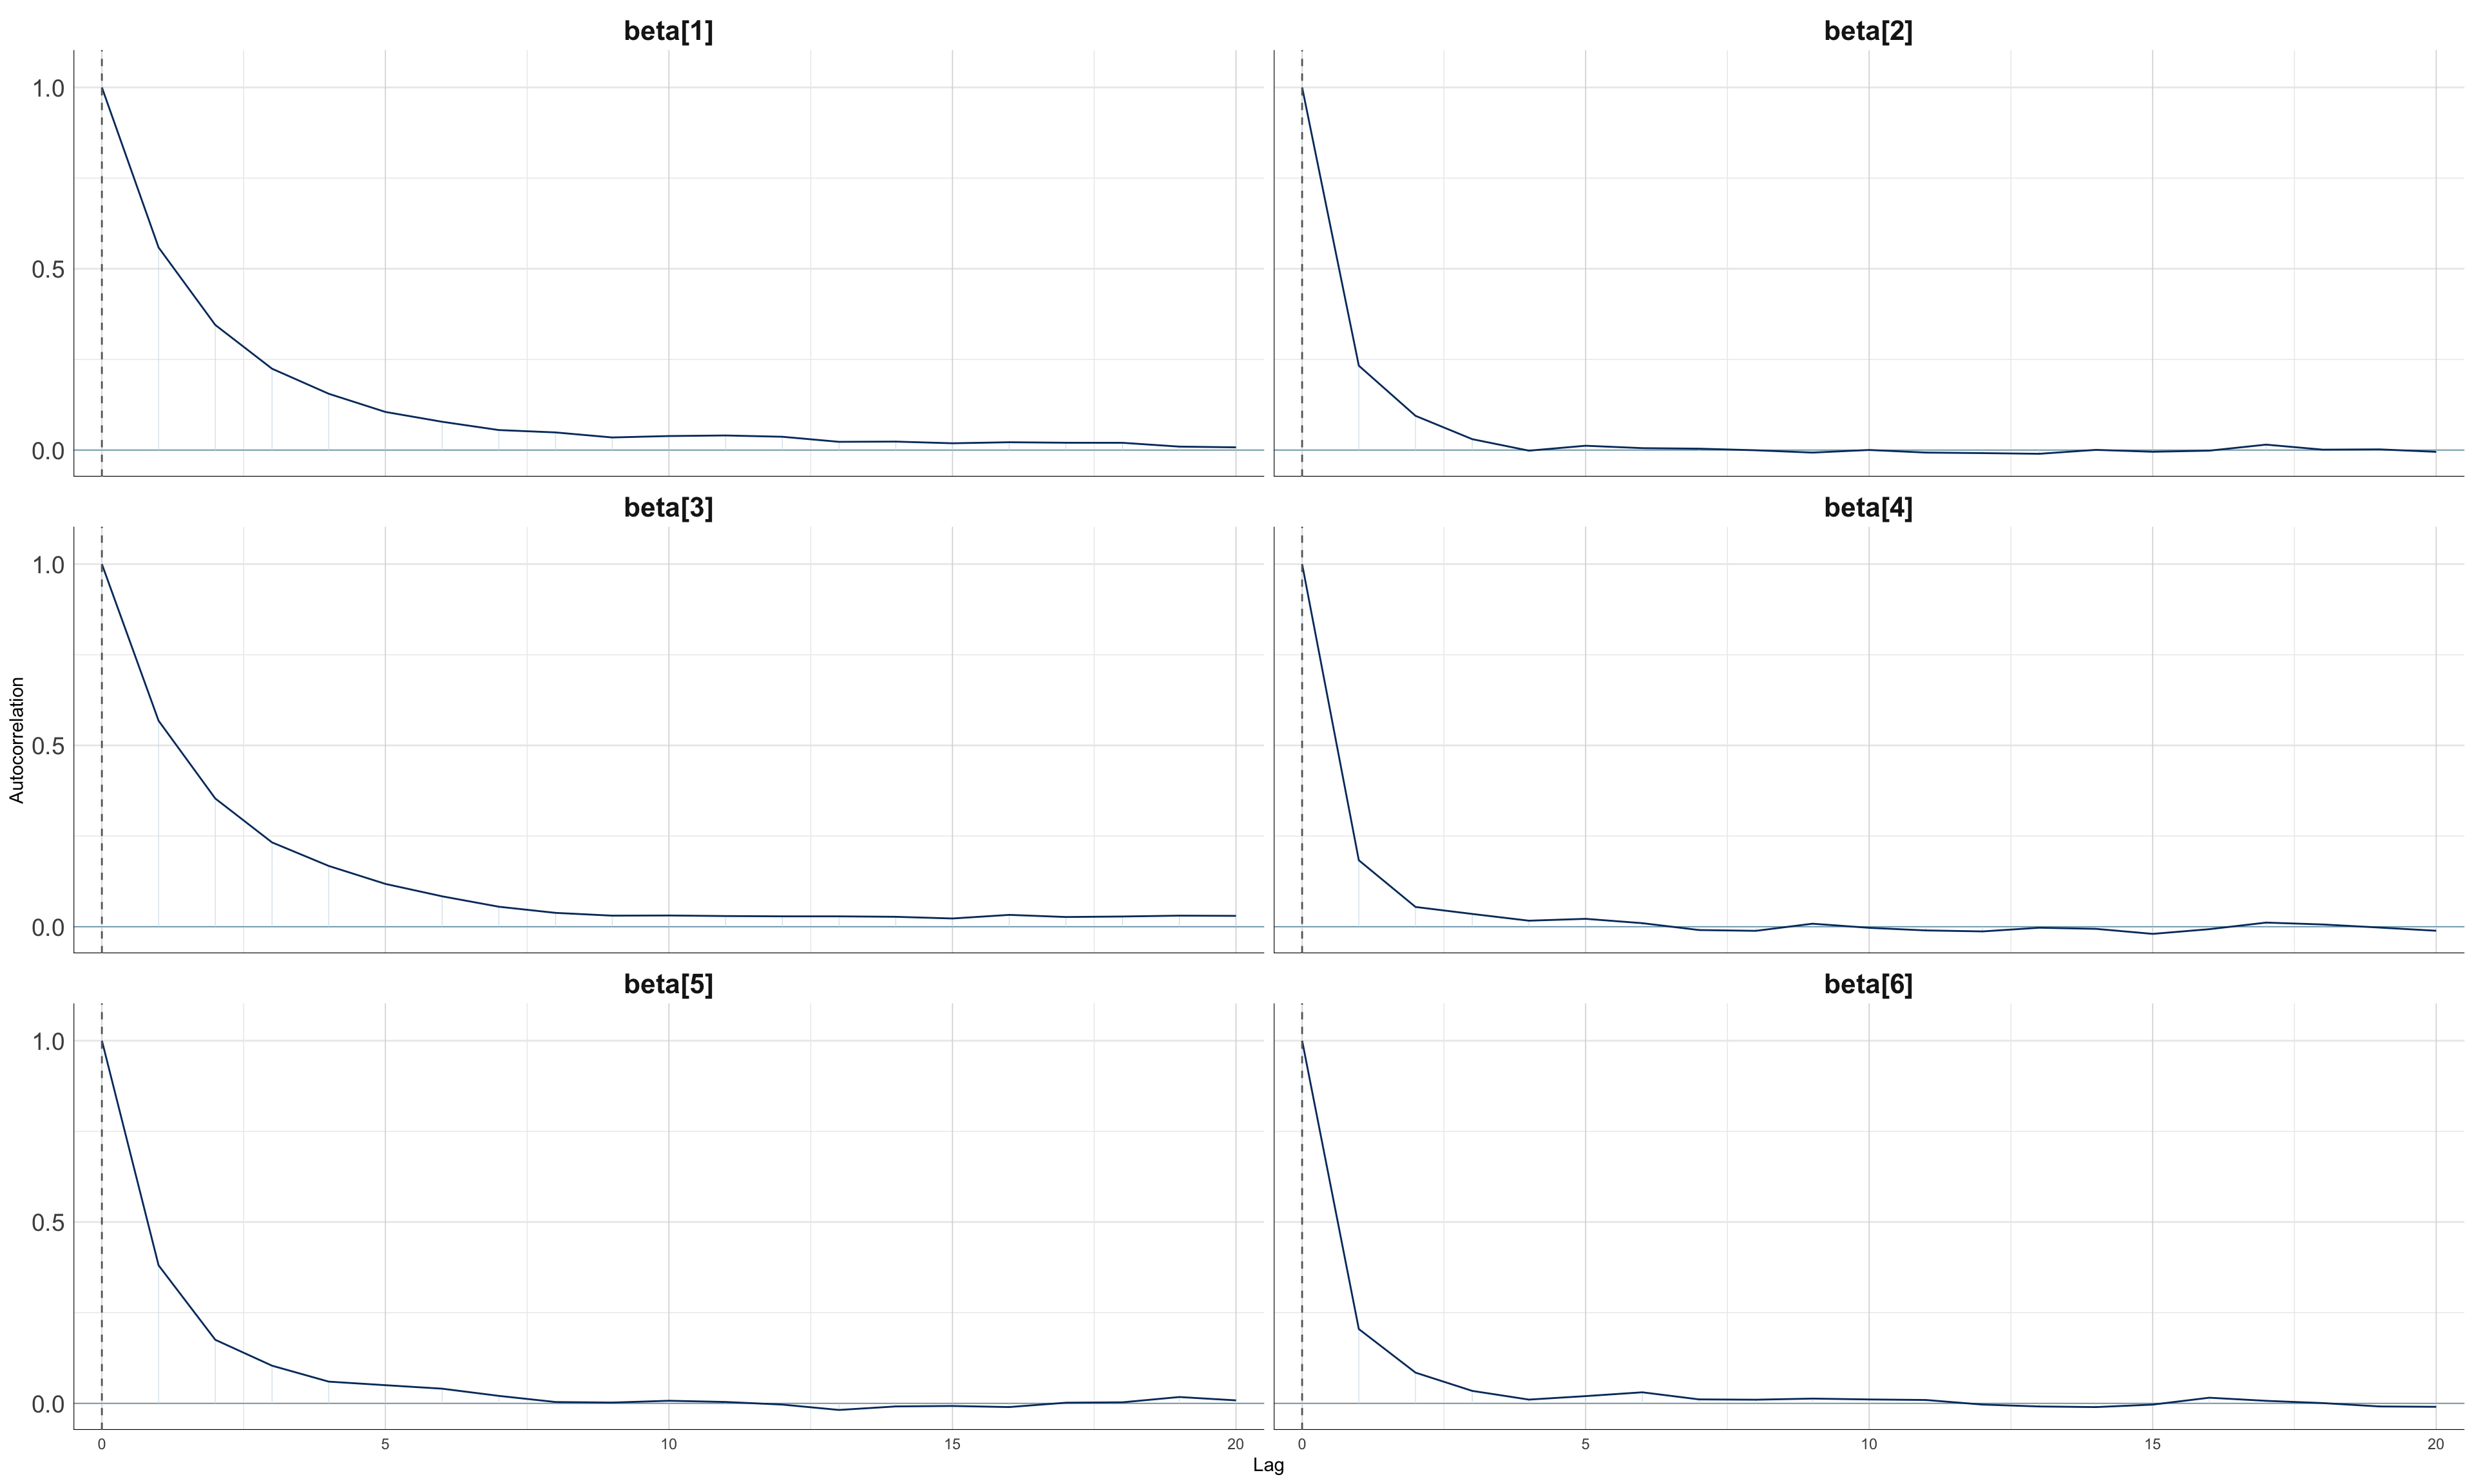
\includegraphics[width=\linewidth]{img/horseshoe_model/acf_beta_chain2_1.png}
    \caption{Group 1.}
  \end{subfigure}\hfill
  \begin{subfigure}[t]{0.48\linewidth}
    \centering
    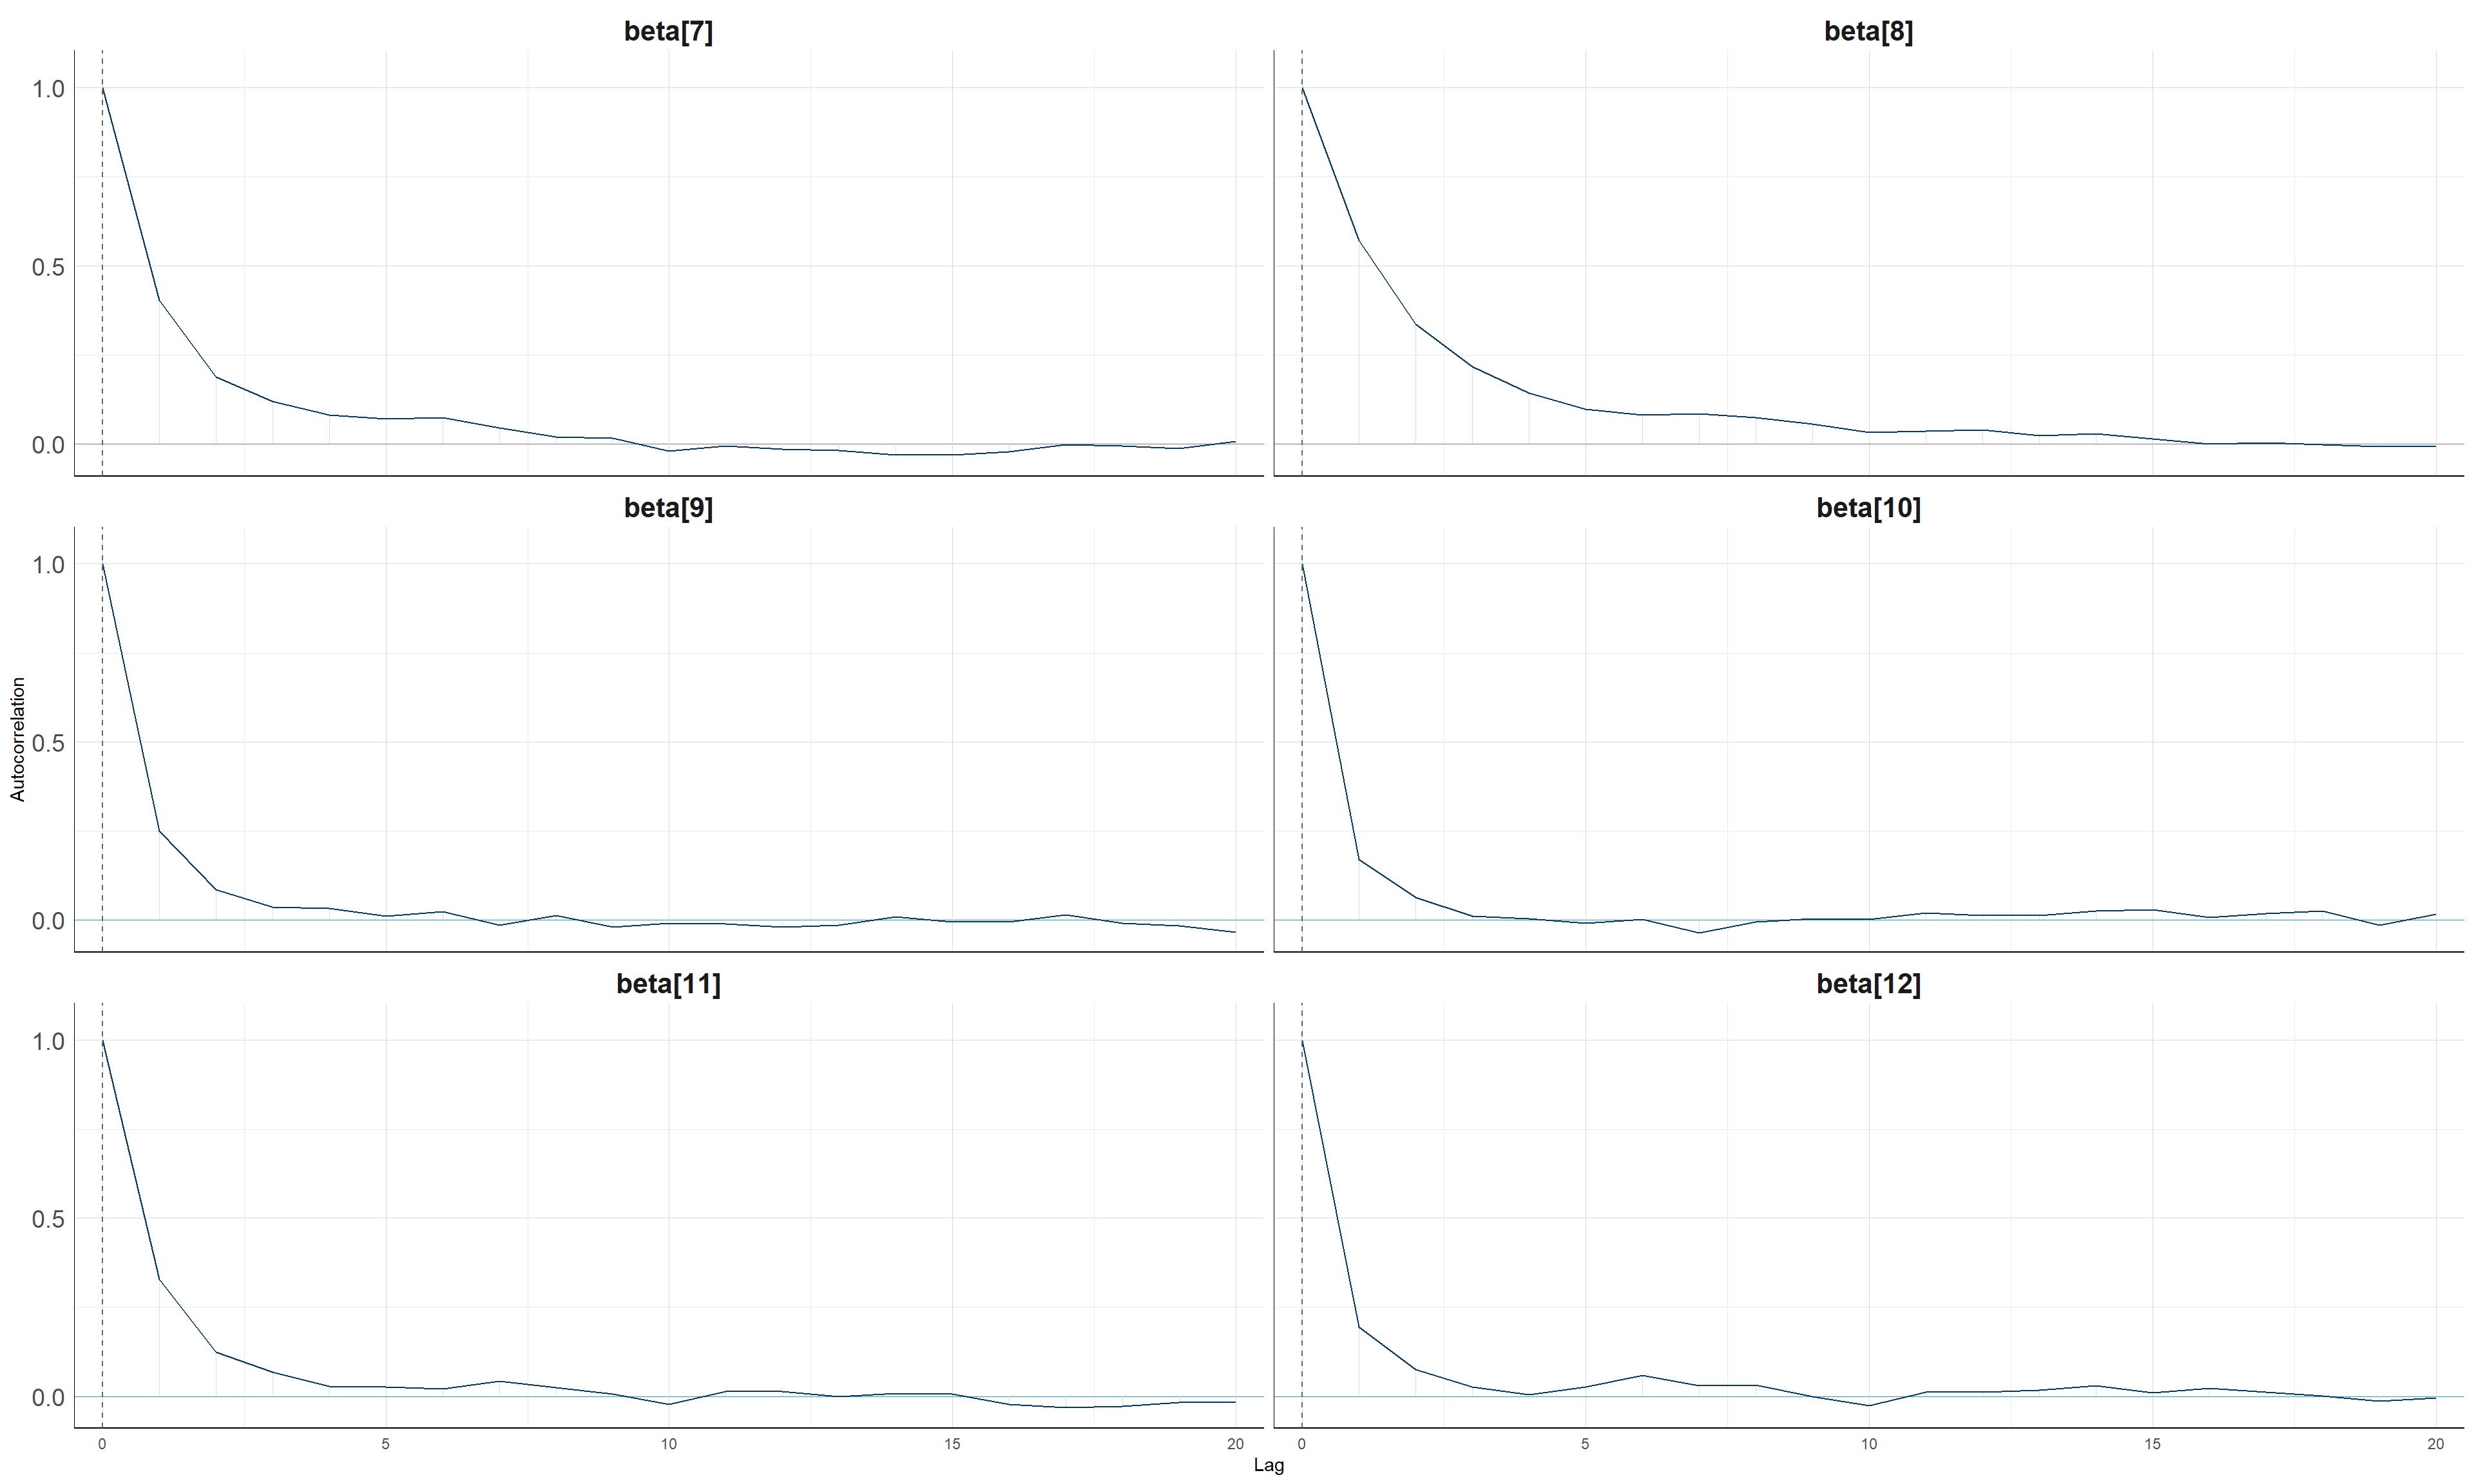
\includegraphics[width=\linewidth]{img/horseshoe_model/acf_beta_chain2_2.png}
    \caption{Group 2.}
  \end{subfigure}\hfill
  \begin{subfigure}[t]{0.48\linewidth}
    \centering
    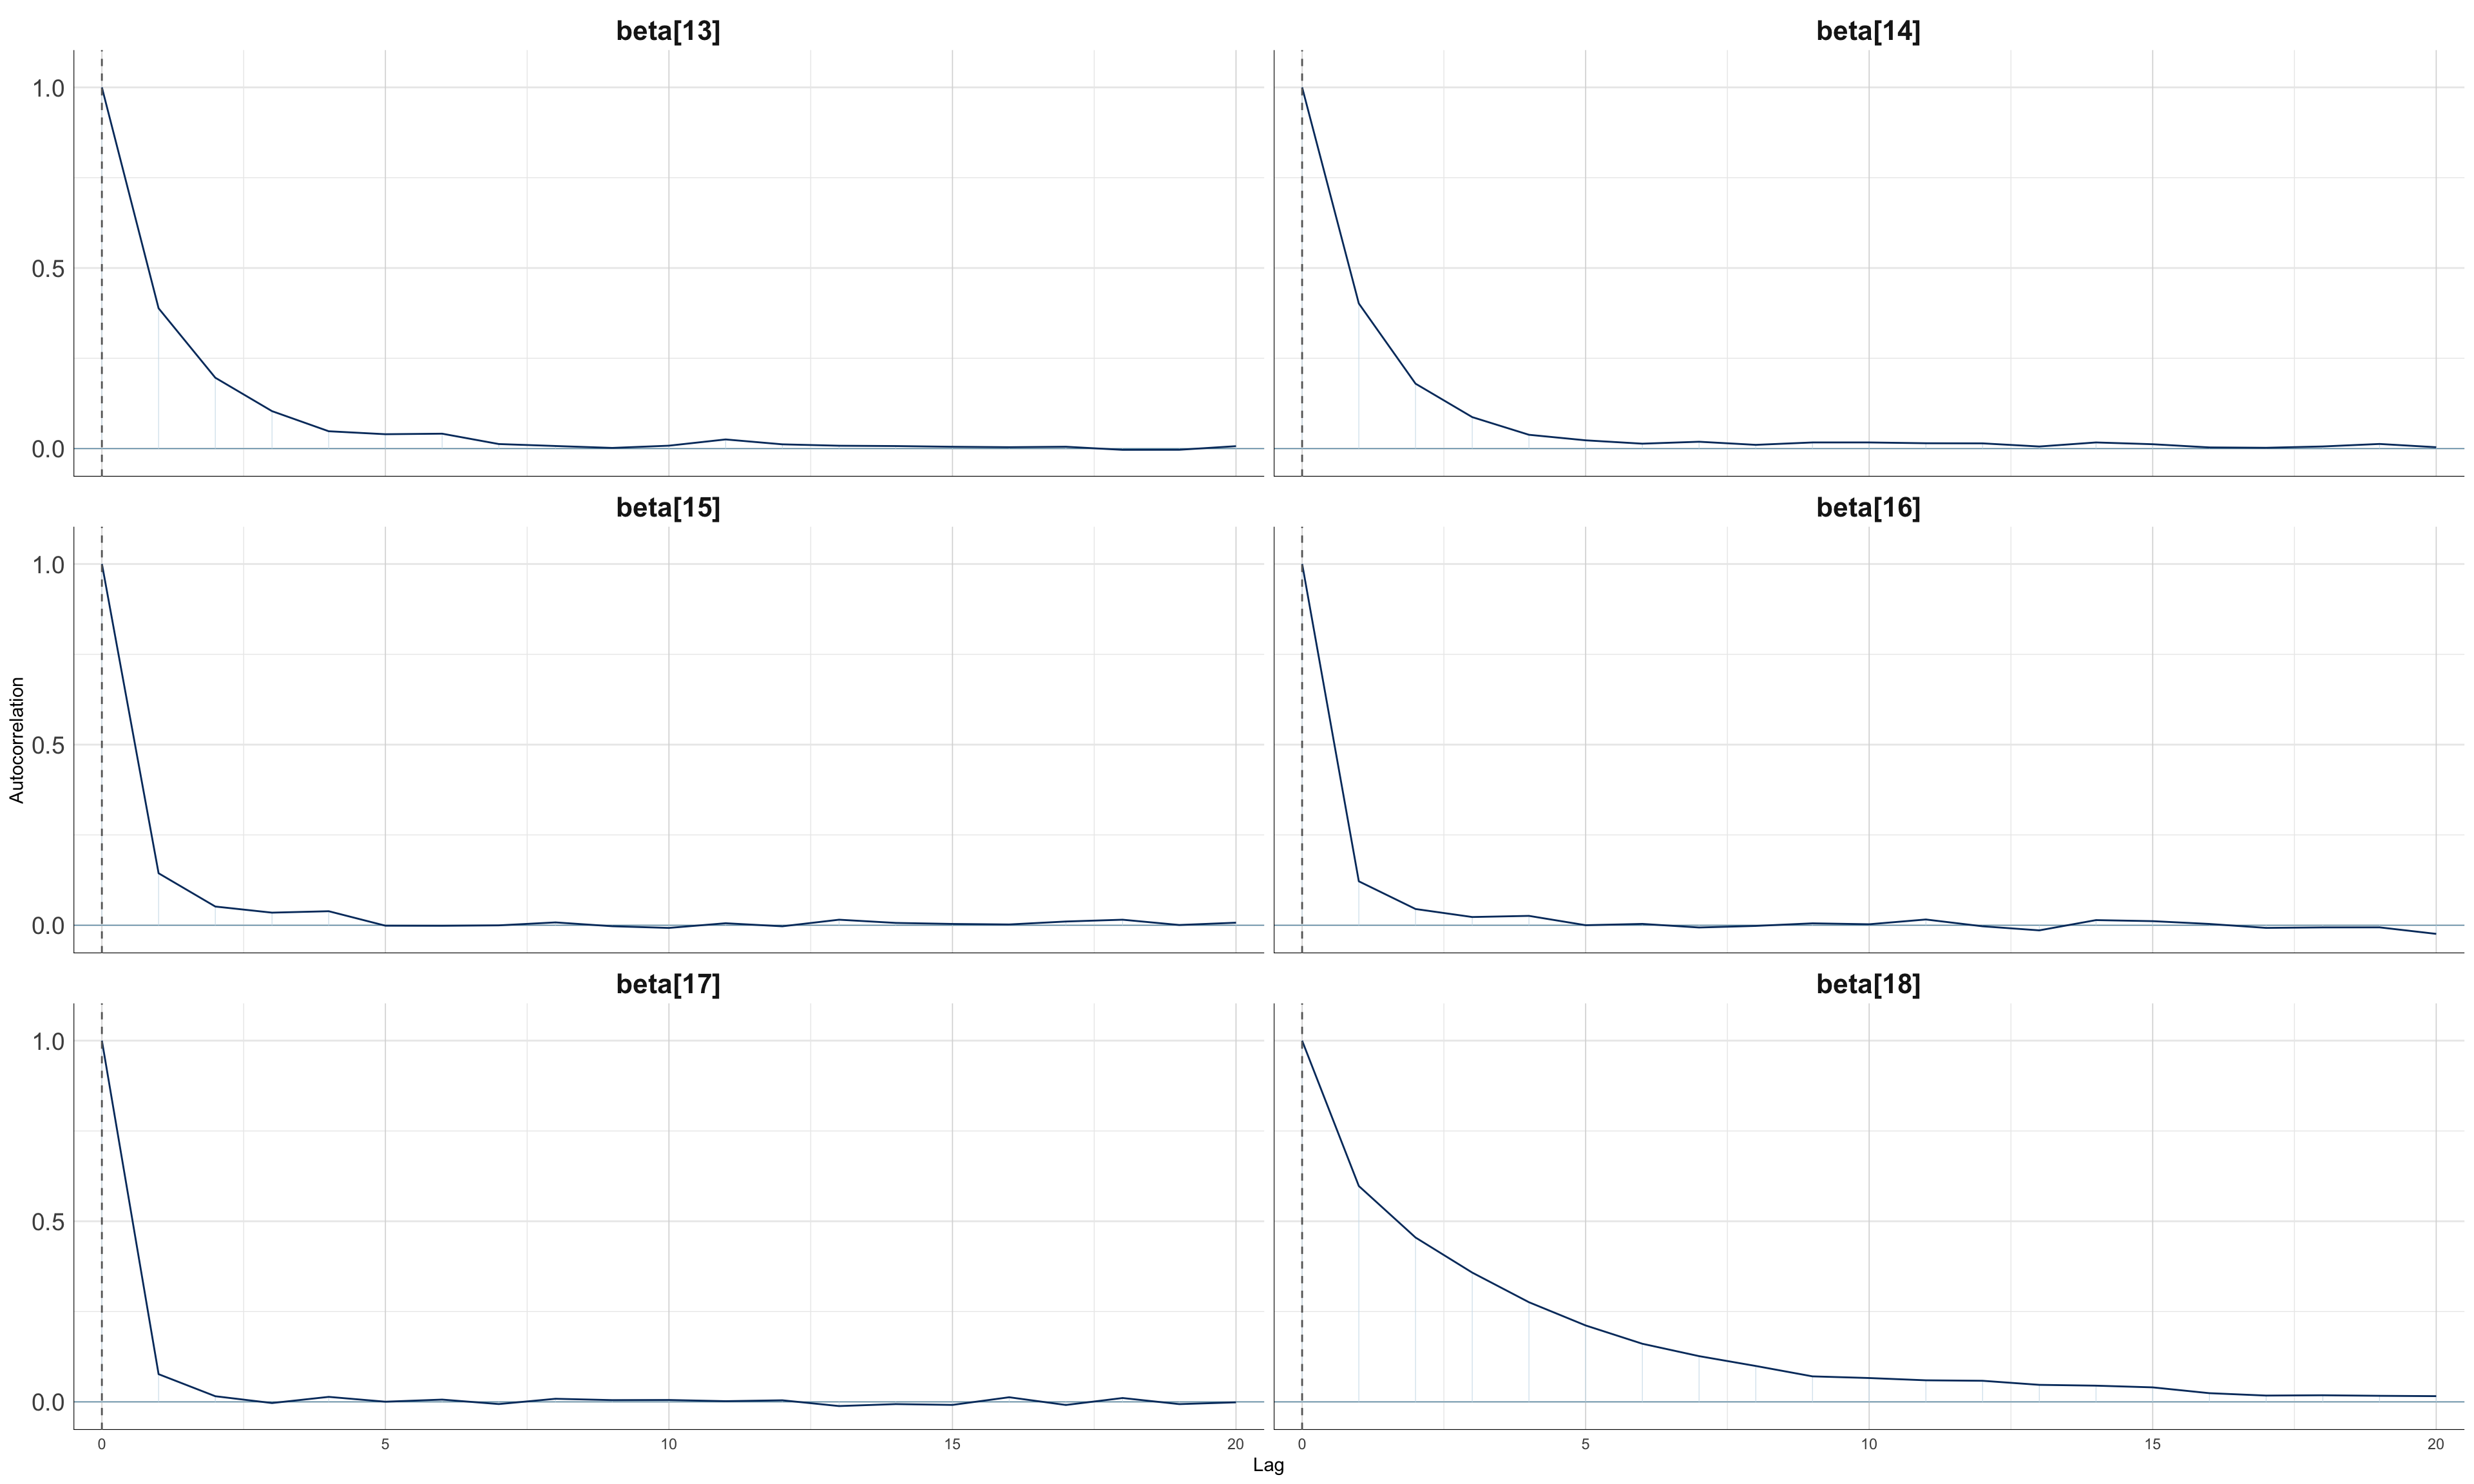
\includegraphics[width=\linewidth]{img/horseshoe_model/acf_beta_chain2_3.png}
    \caption{Group 3.}
  \end{subfigure}\hfill
  \begin{subfigure}[t]{0.48\linewidth}
    \centering
    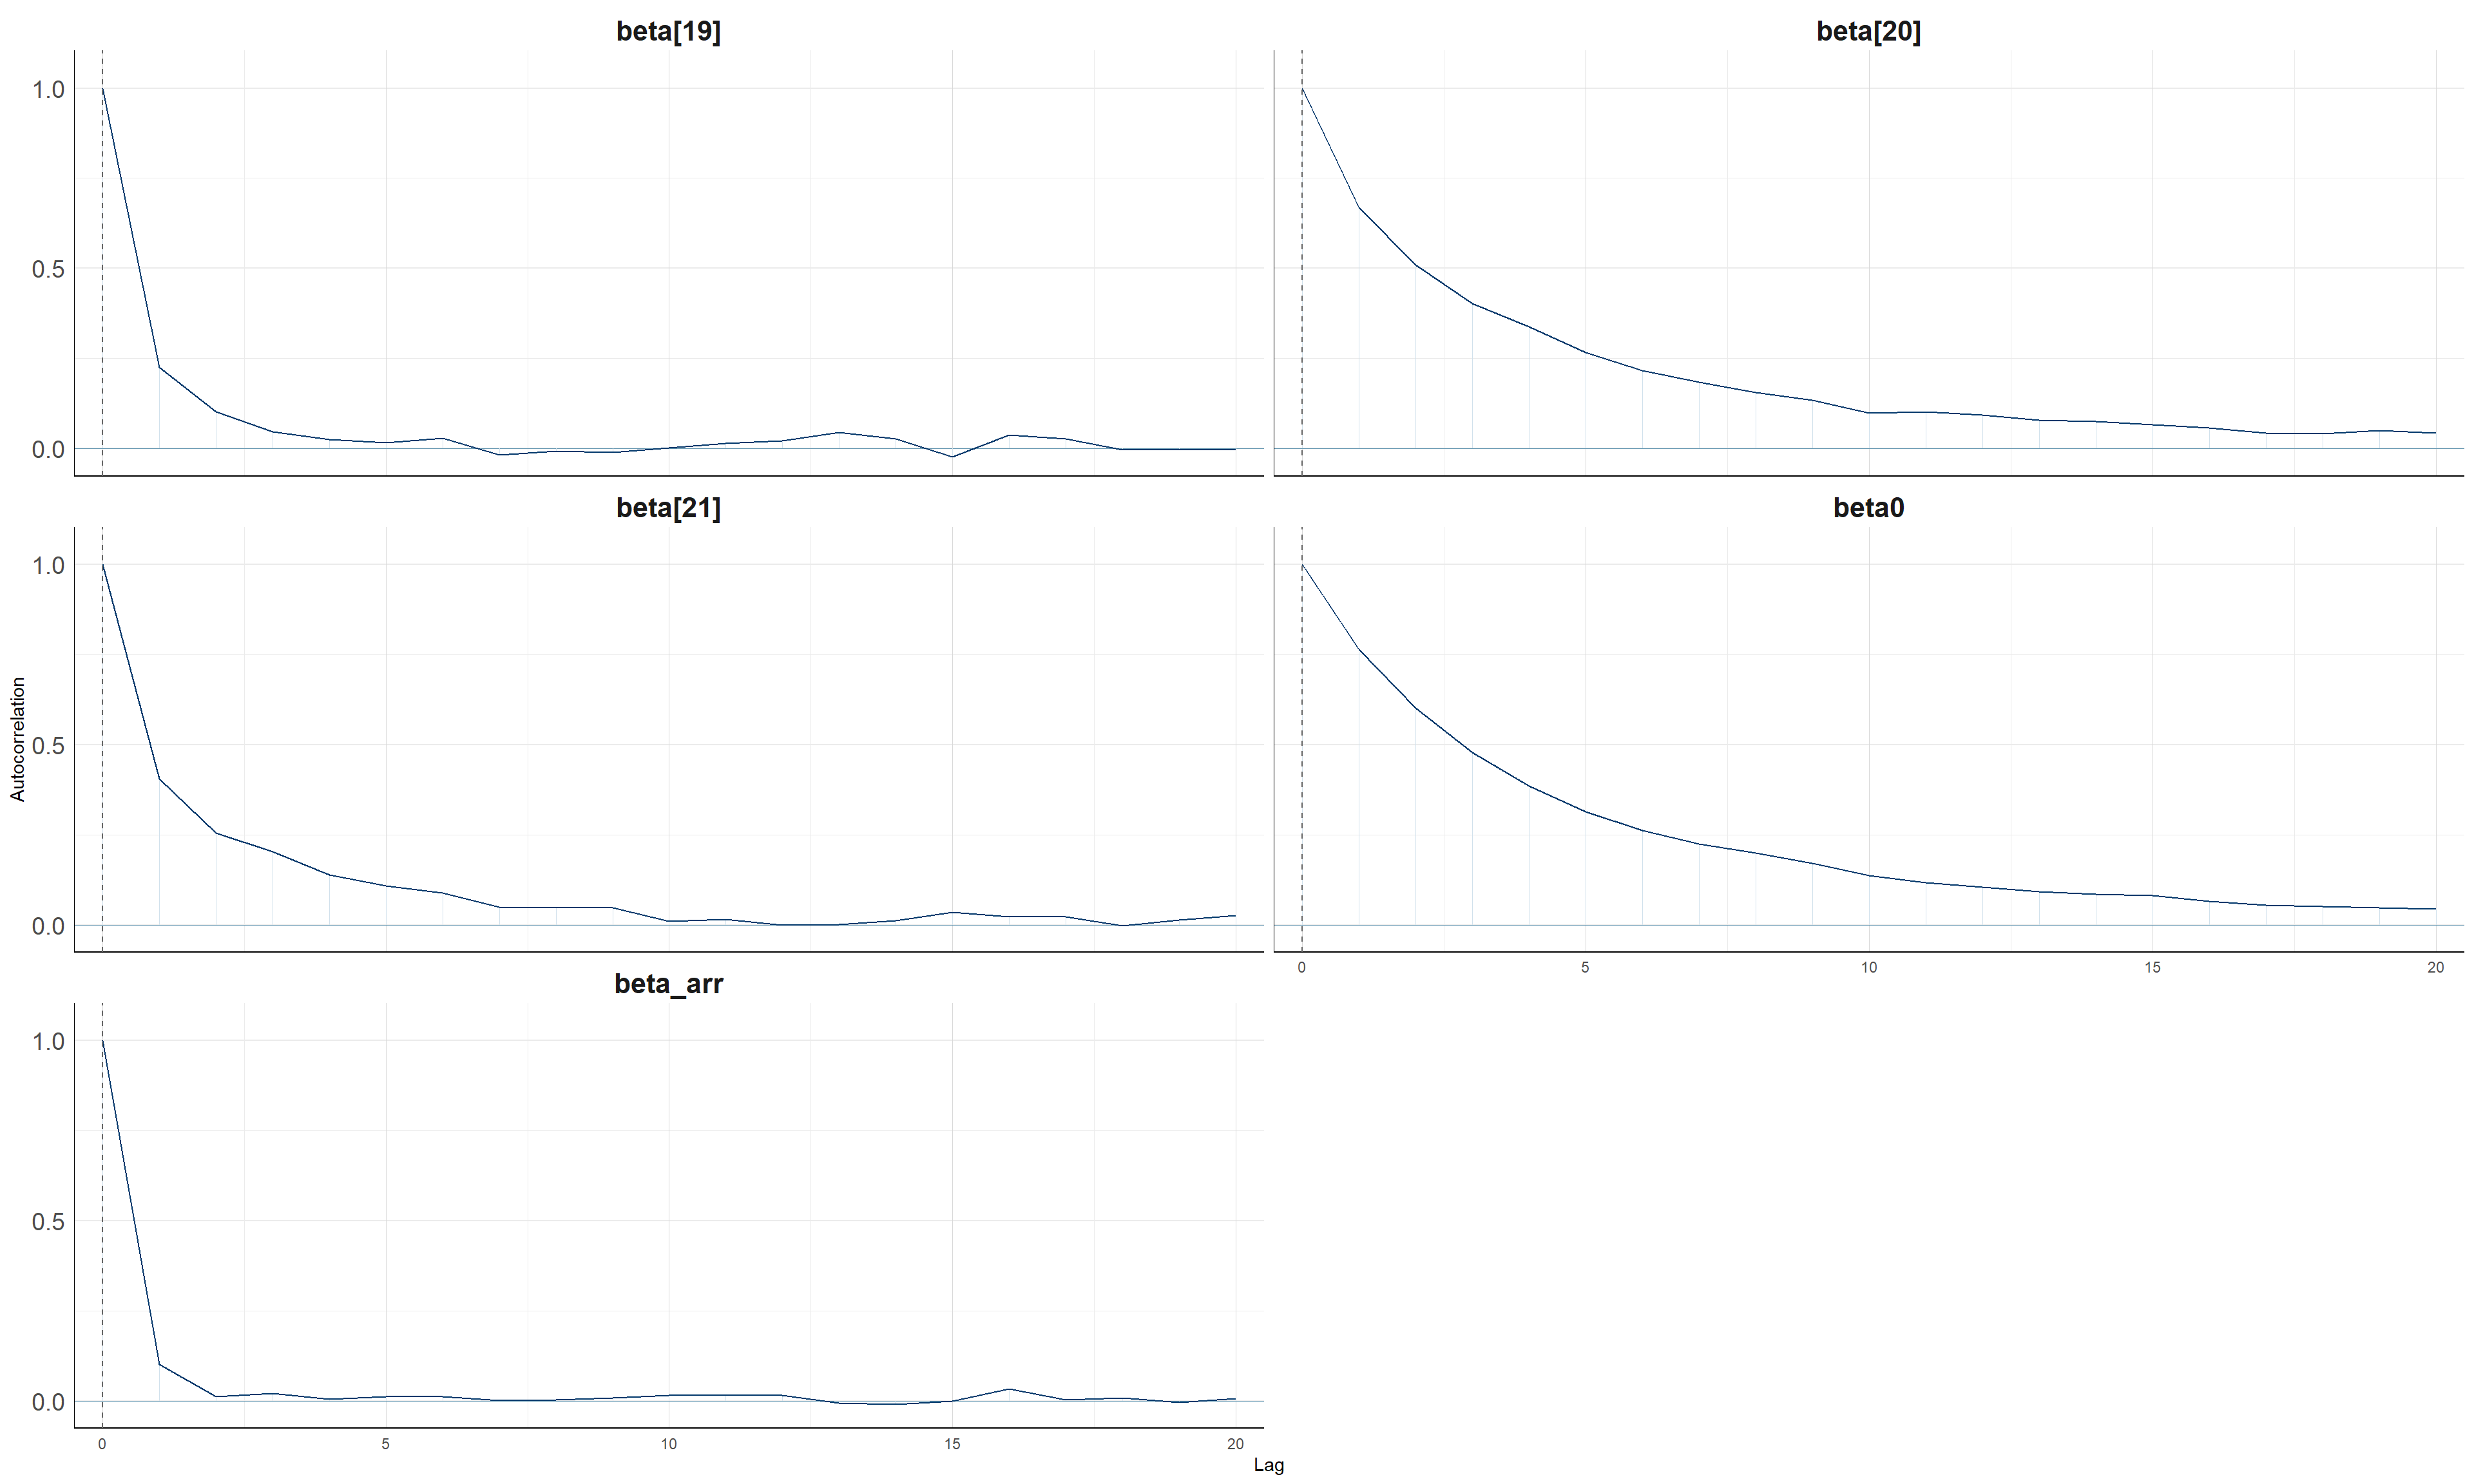
\includegraphics[width=\linewidth]{img/horseshoe_model/acf_beta_chain2_4.png}
    \caption{Group 4.}
  \end{subfigure}\hfill
  \caption{Autocorrelation of the coefficients $\beta_j$, chain 2.}
  \label{fig:hs_acf_beta_2}
\end{figure}

\begin{figure}[htbp]
  \centering
  \begin{subfigure}[t]{0.48\linewidth}
    \centering
    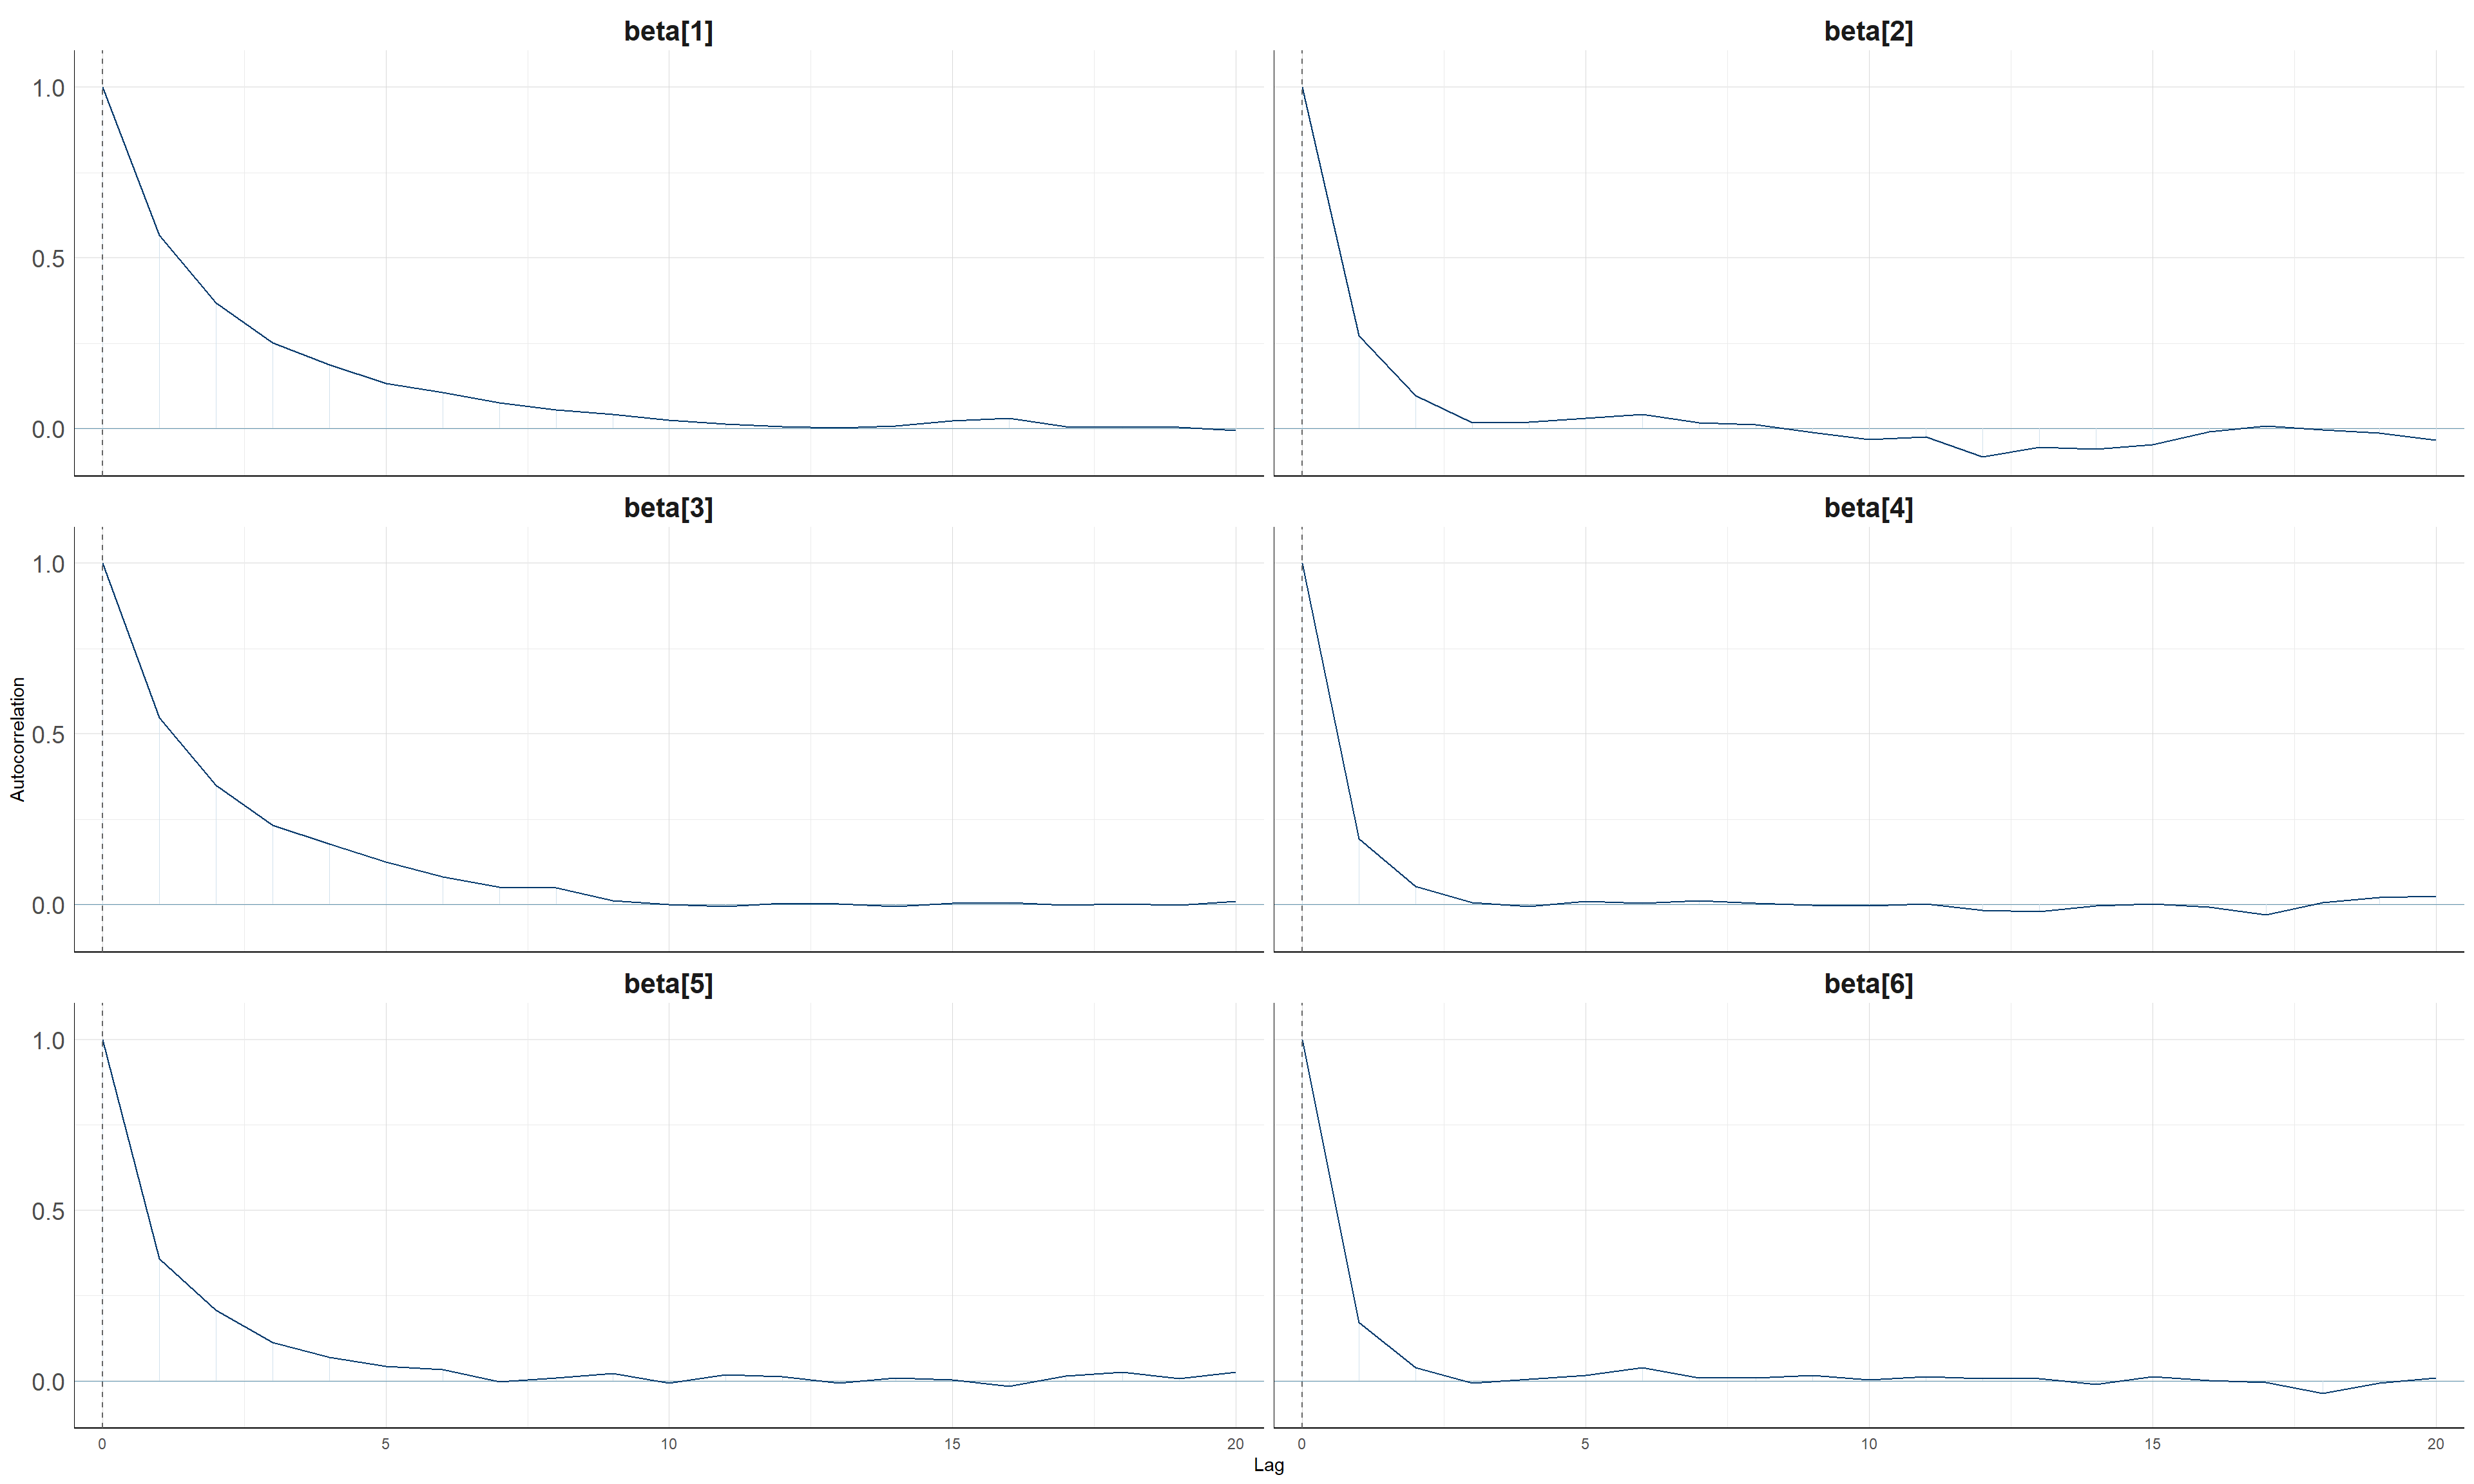
\includegraphics[width=\linewidth]{img/horseshoe_model/acf_beta_chain3_1.png}
    \caption{Group 1.}
  \end{subfigure}\hfill
  \begin{subfigure}[t]{0.48\linewidth}
    \centering
    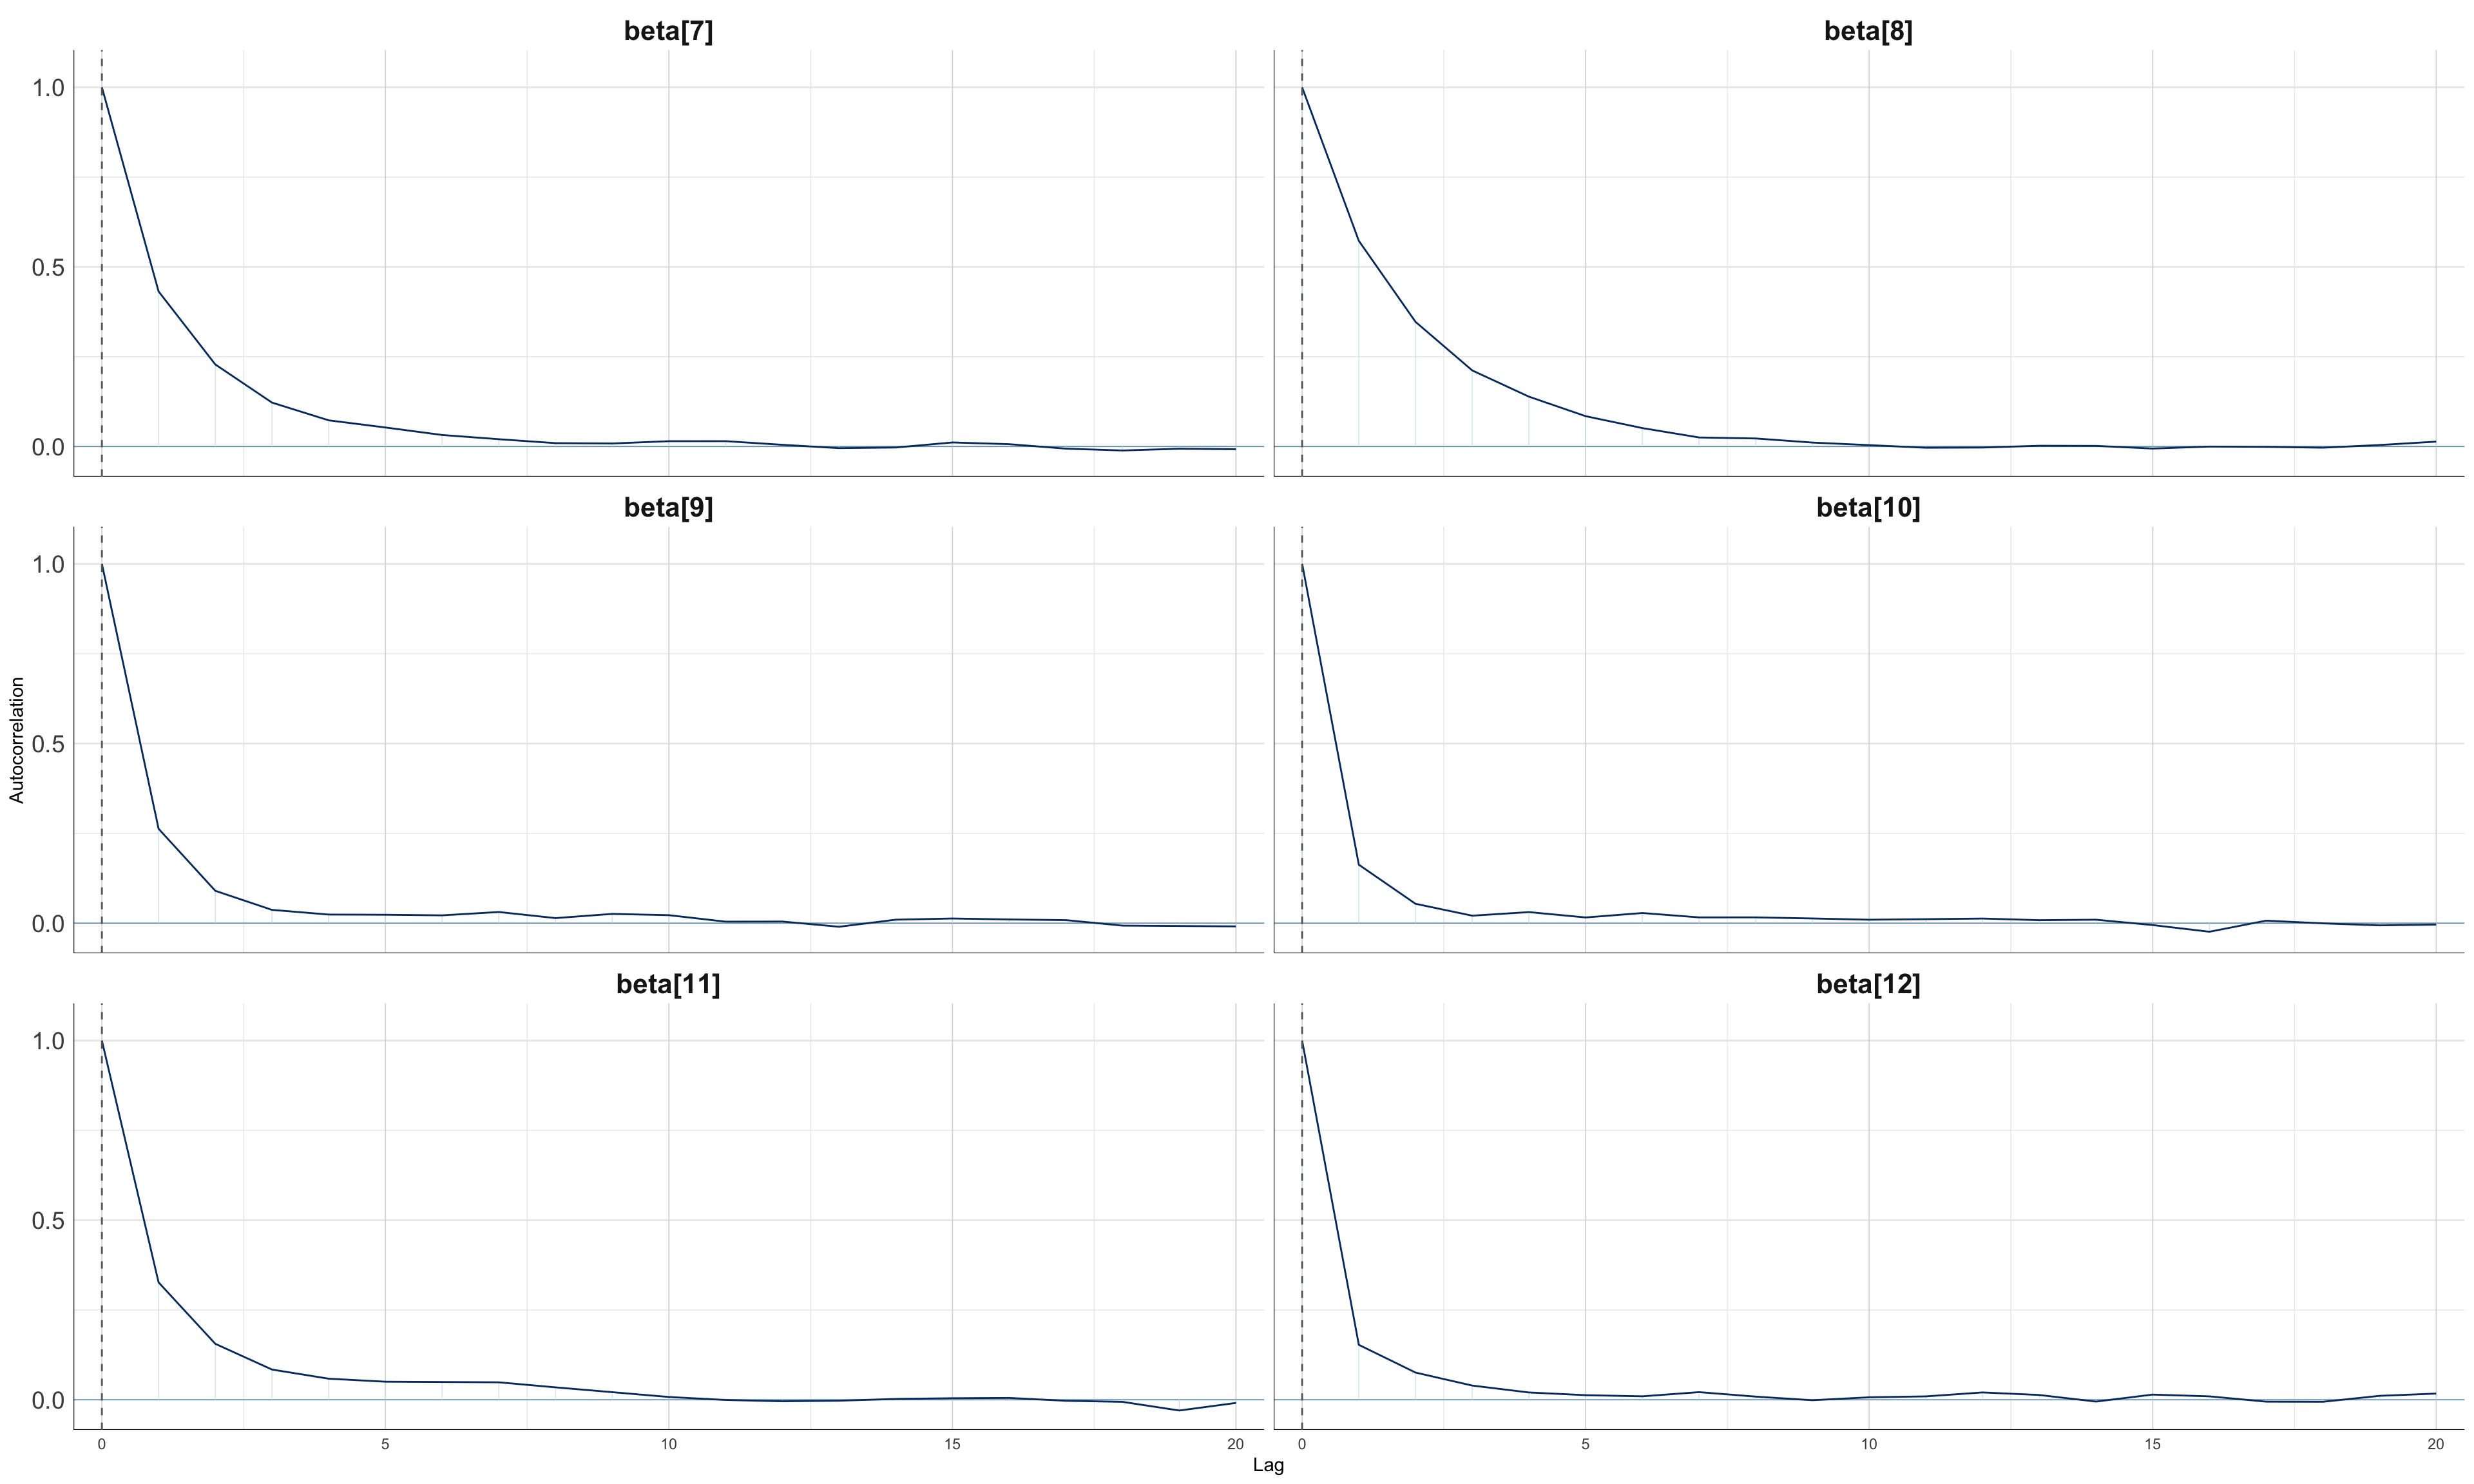
\includegraphics[width=\linewidth]{img/horseshoe_model/acf_beta_chain3_2.png}
    \caption{Group 2.}
  \end{subfigure}\hfill
  \begin{subfigure}[t]{0.48\linewidth}
    \centering
    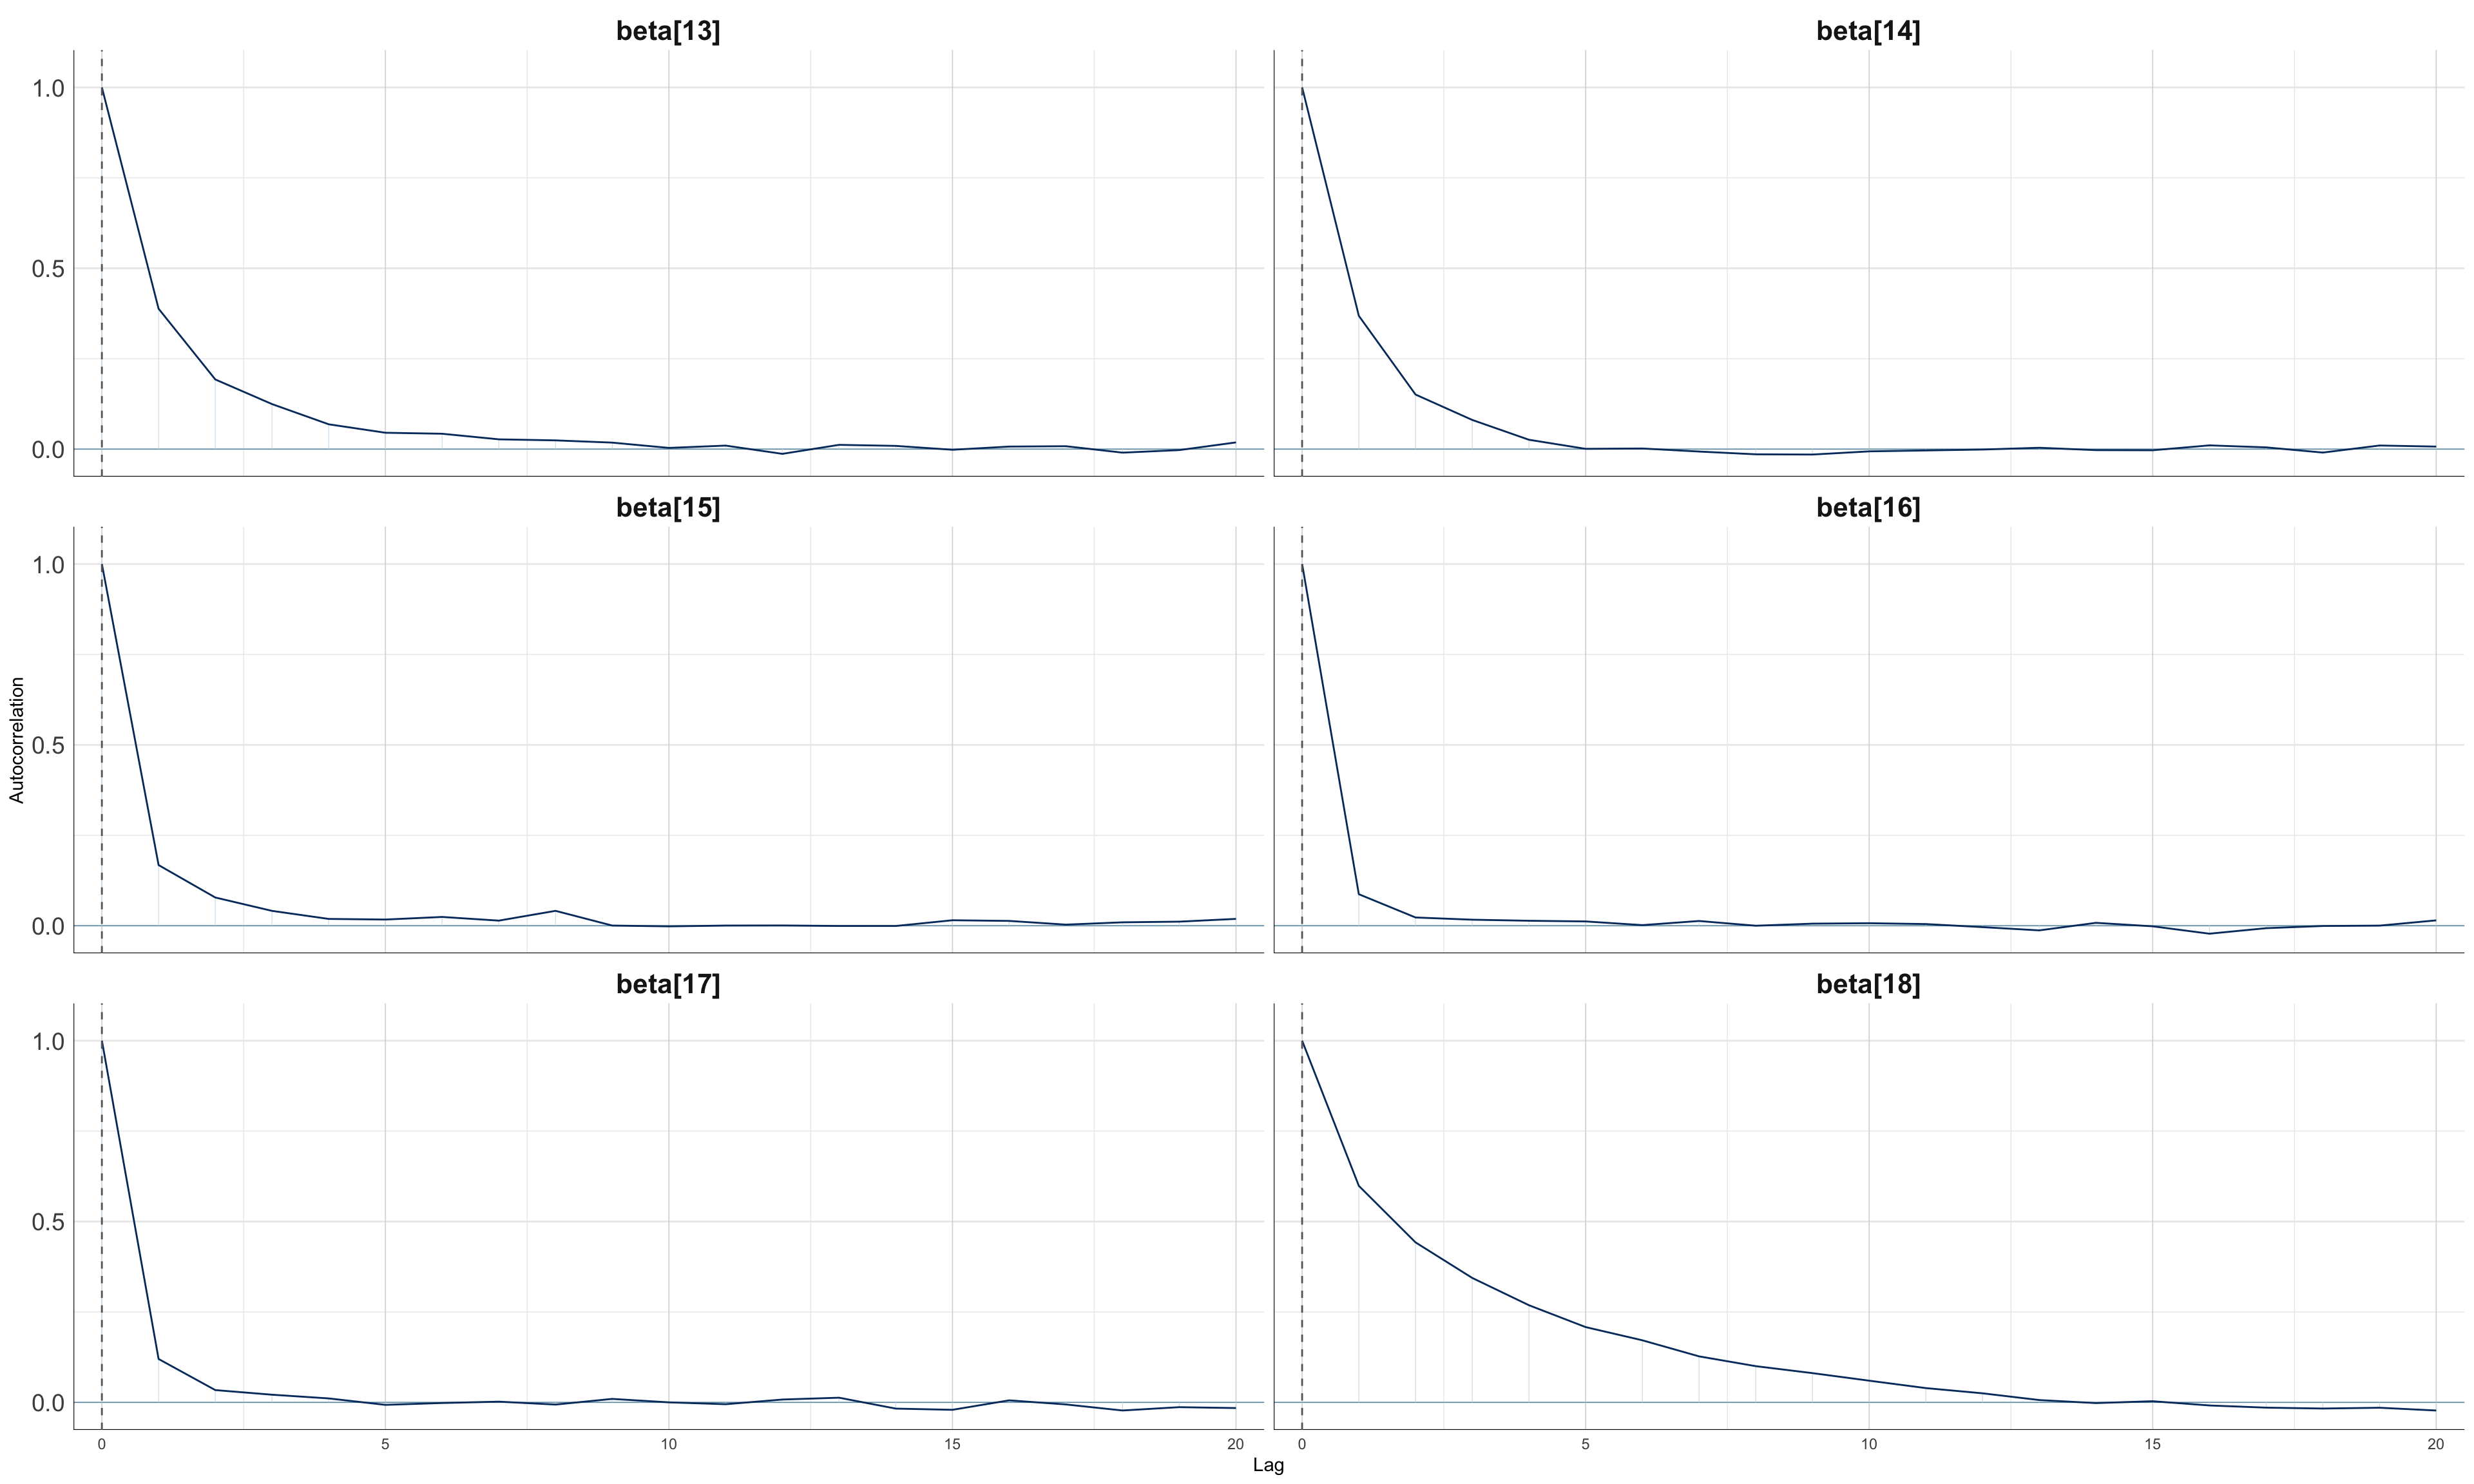
\includegraphics[width=\linewidth]{img/horseshoe_model/acf_beta_chain3_3.png}
    \caption{Group 3.}
  \end{subfigure}\hfill
  \begin{subfigure}[t]{0.48\linewidth}
    \centering
    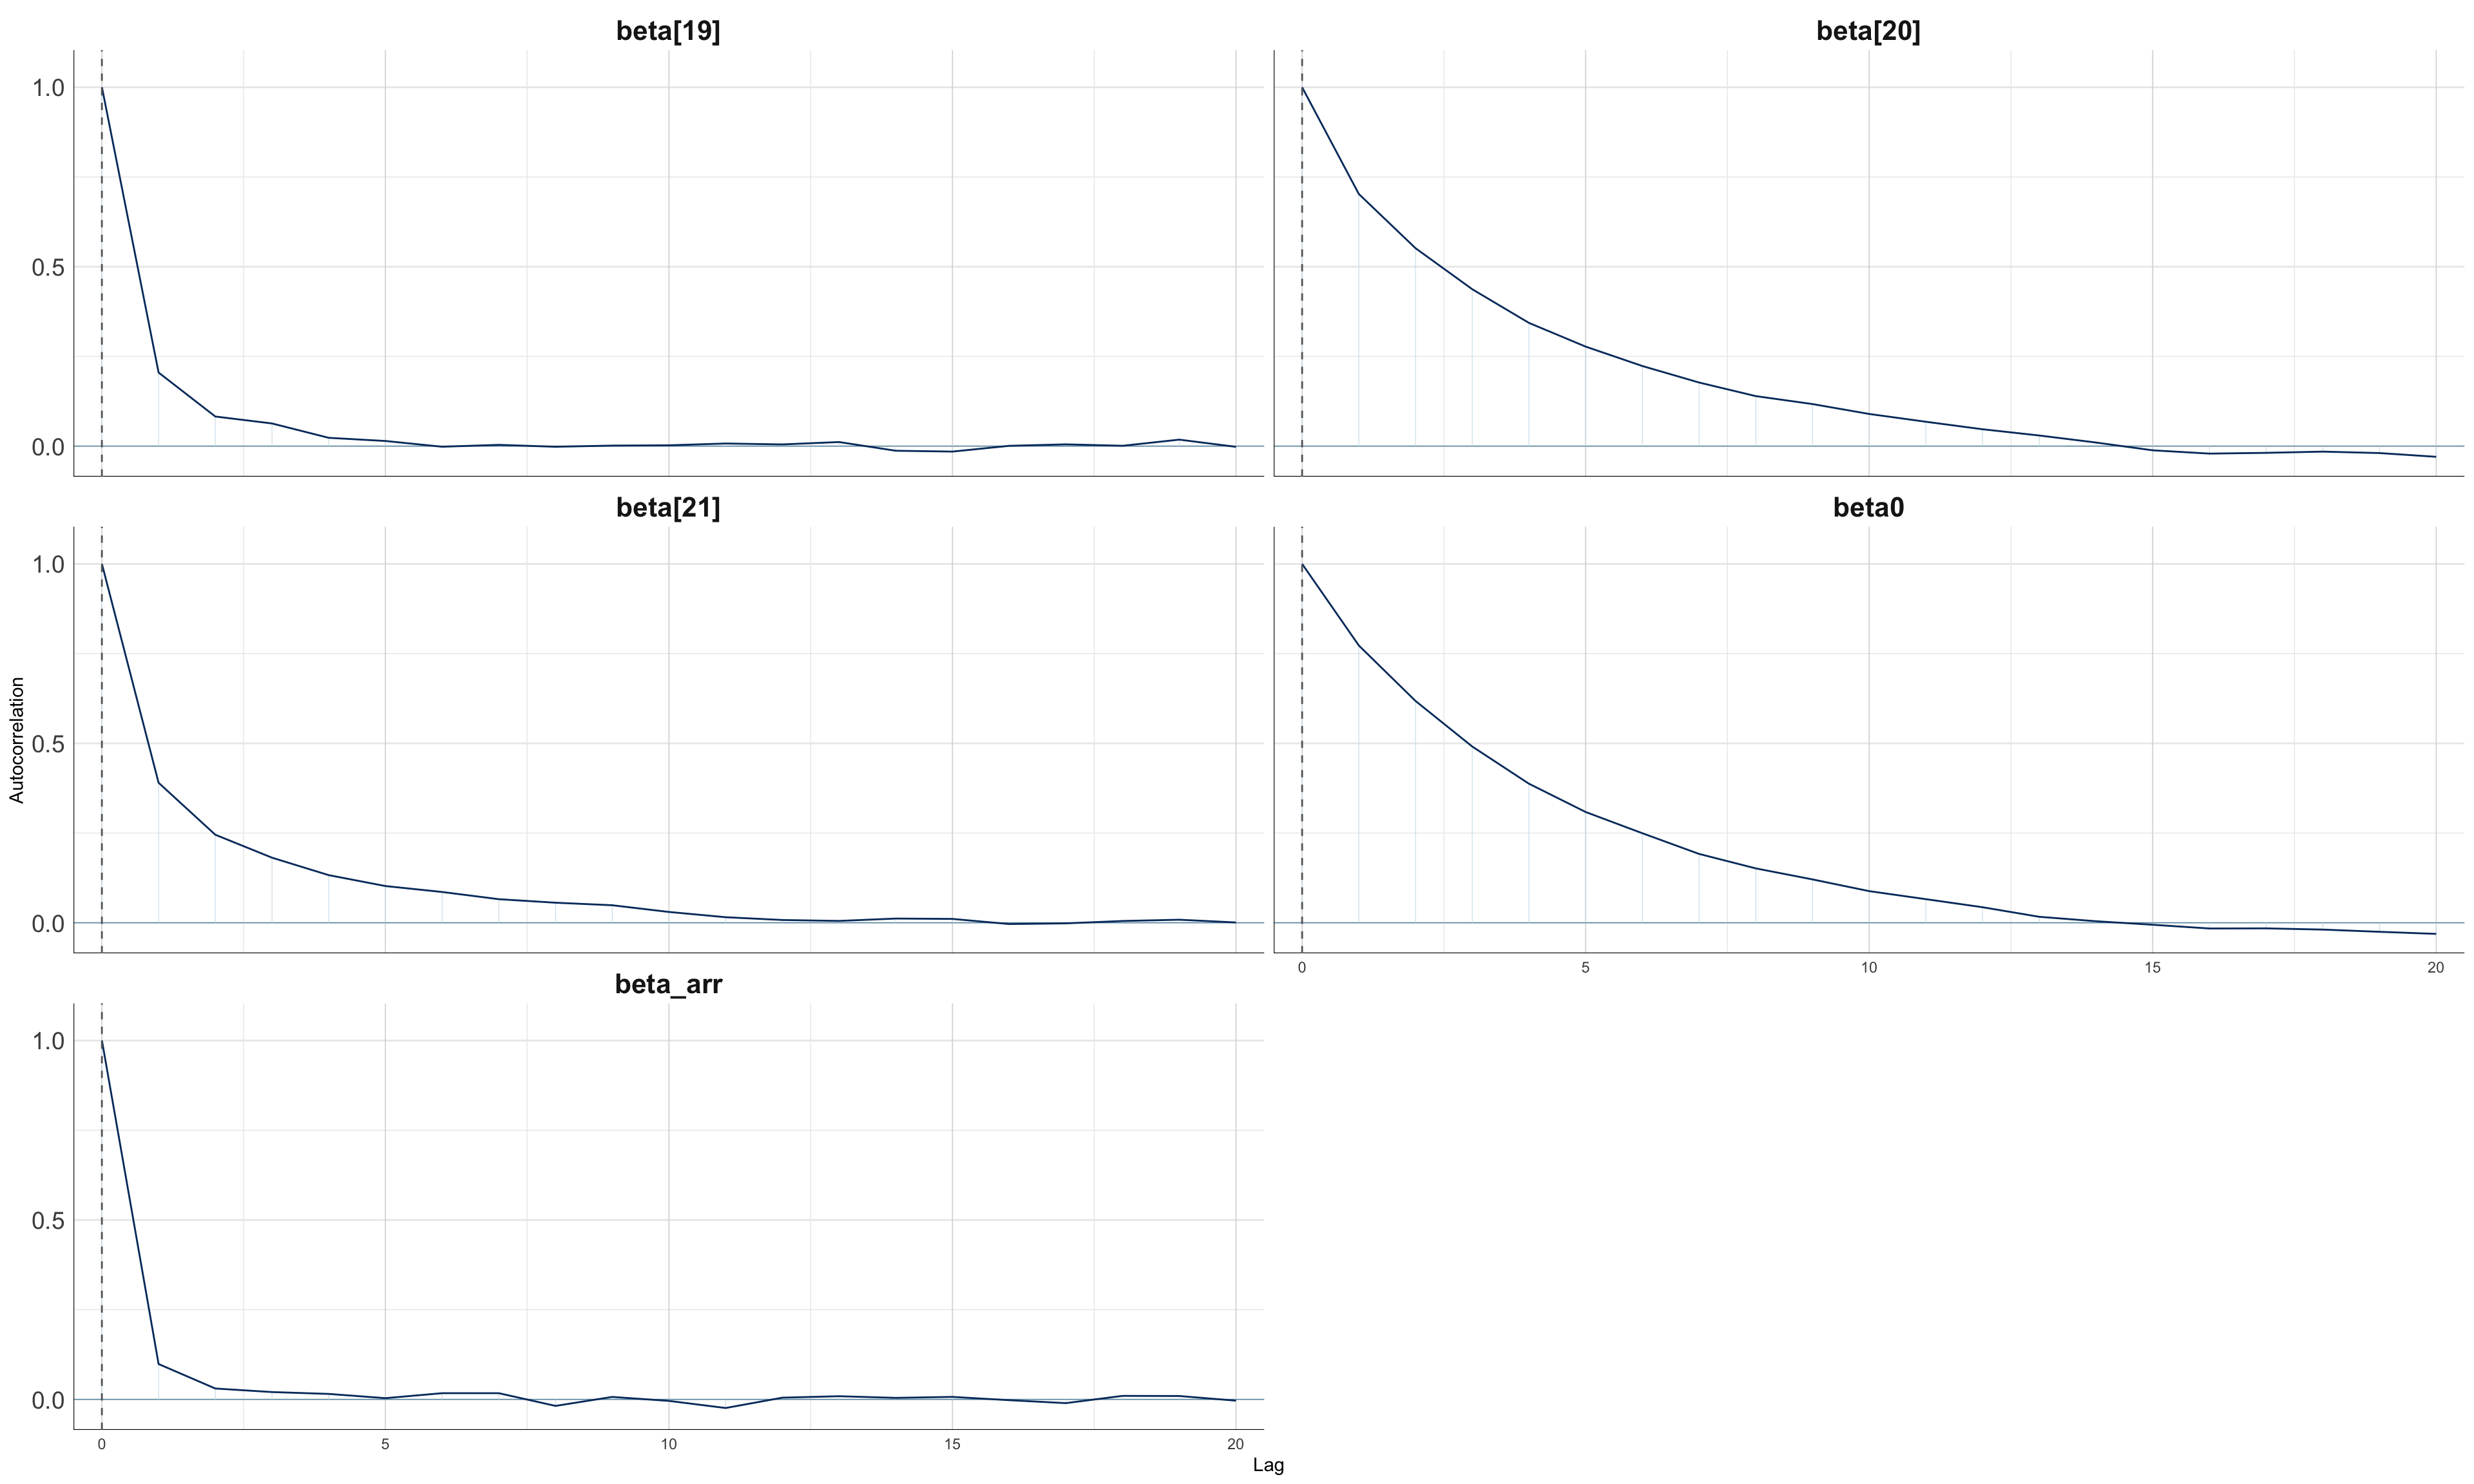
\includegraphics[width=\linewidth]{img/horseshoe_model/acf_beta_chain3_4.png}
    \caption{Group 4.}
  \end{subfigure}\hfill
  \caption{Autocorrelation of the coefficients $\beta_j$, chain 3.}
  \label{fig:hs_acf_beta_3}
\end{figure}

\begin{figure}[htbp]
  \centering
  \begin{subfigure}[t]{0.48\linewidth}
    \centering
    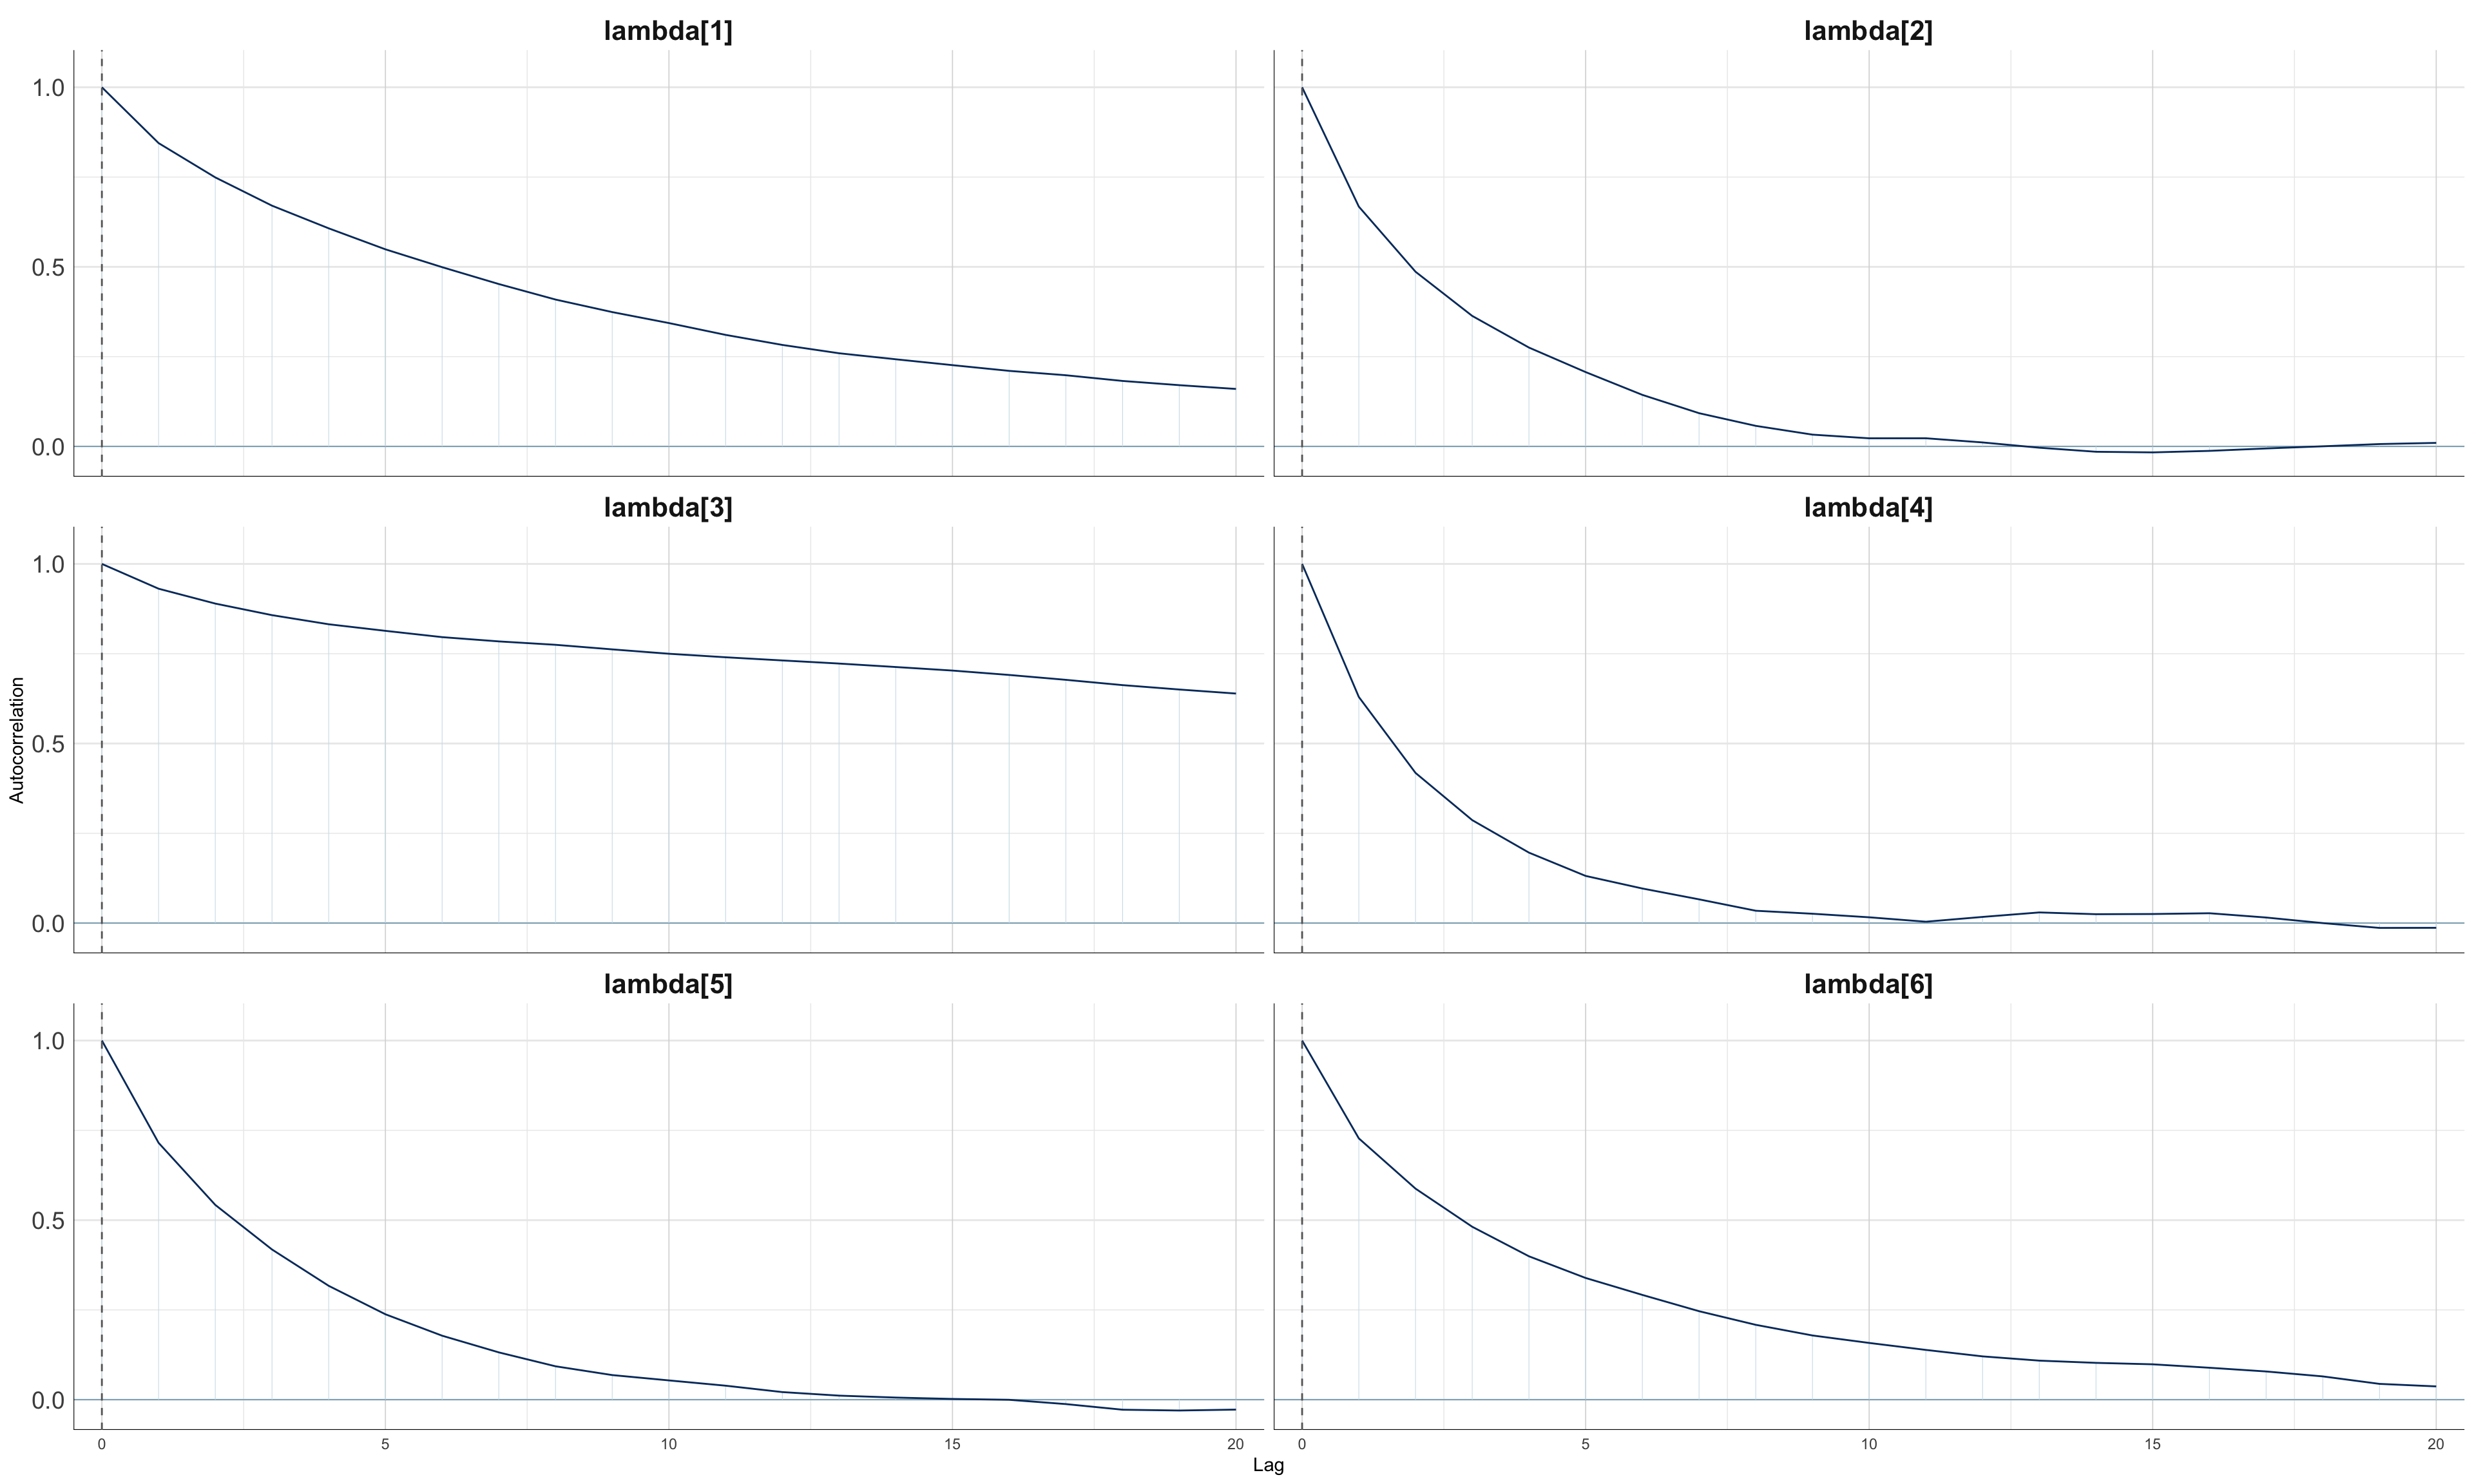
\includegraphics[width=\linewidth]{img/horseshoe_model/acf_lambda_chain1_1.png}
    \caption{Group 1.}
  \end{subfigure}\hfill
  \begin{subfigure}[t]{0.48\linewidth}
    \centering
    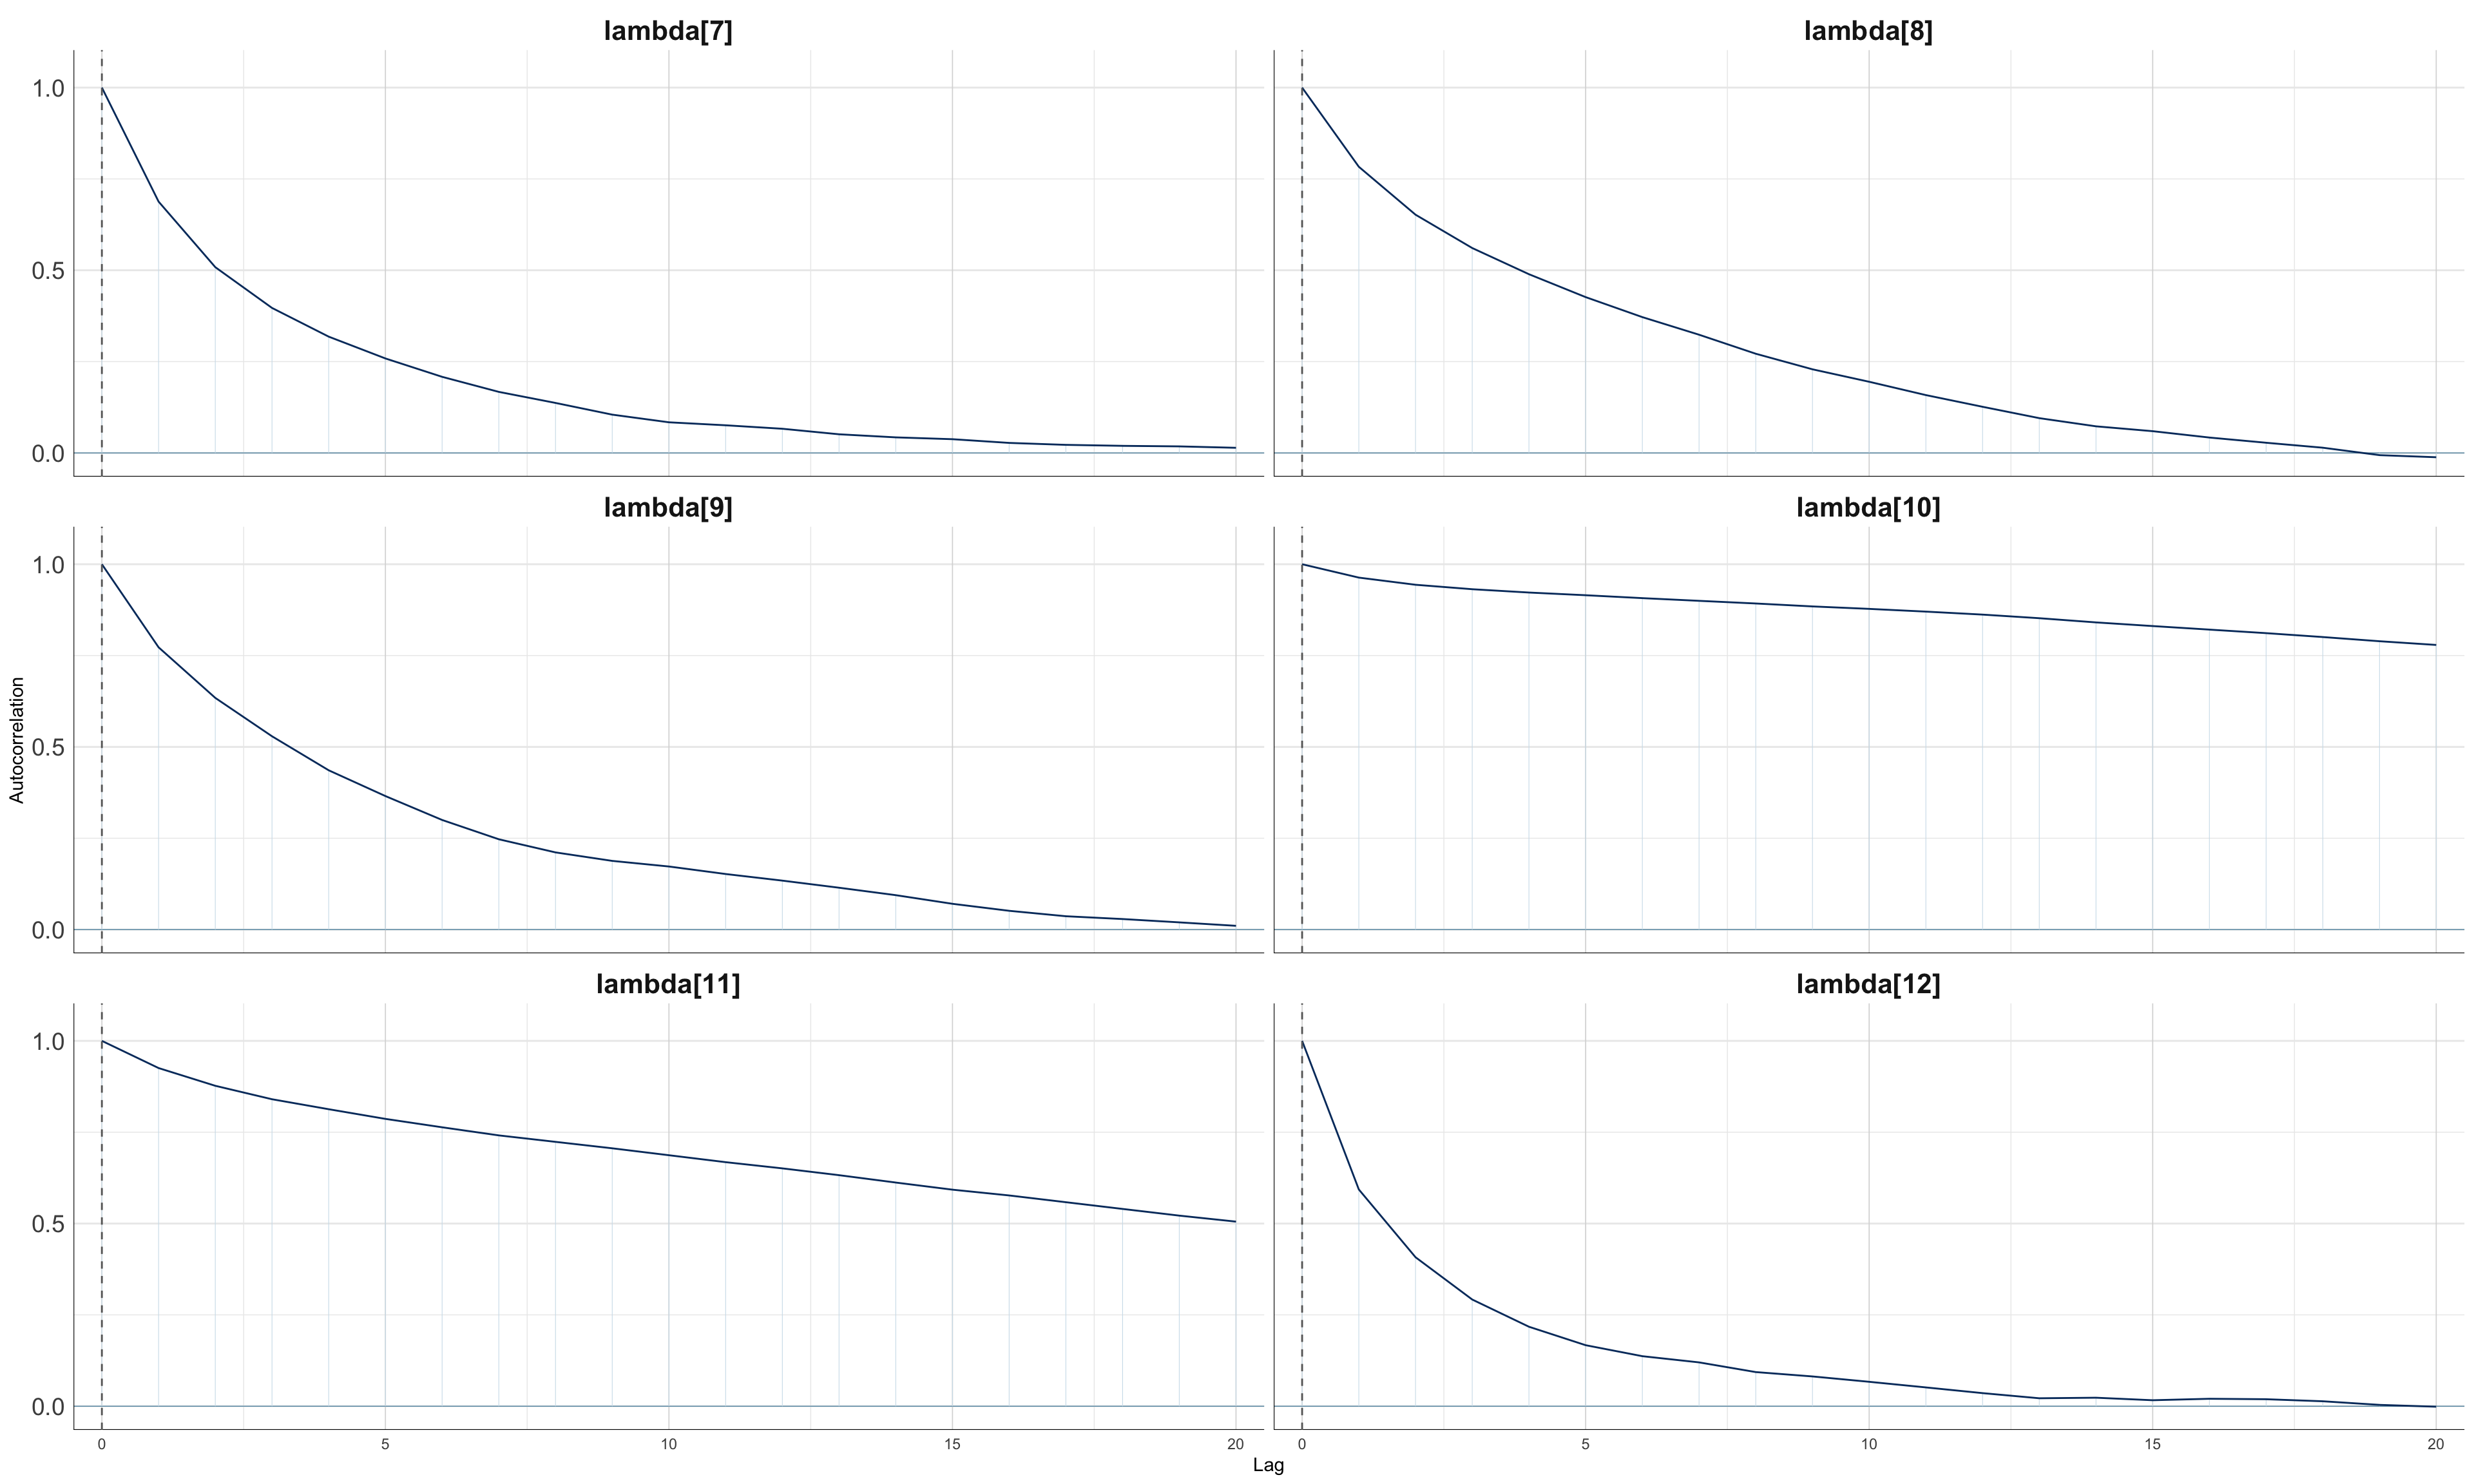
\includegraphics[width=\linewidth]{img/horseshoe_model/acf_lambda_chain1_2.png}
    \caption{Group 2.}
  \end{subfigure}\hfill
  \begin{subfigure}[t]{0.48\linewidth}
    \centering
    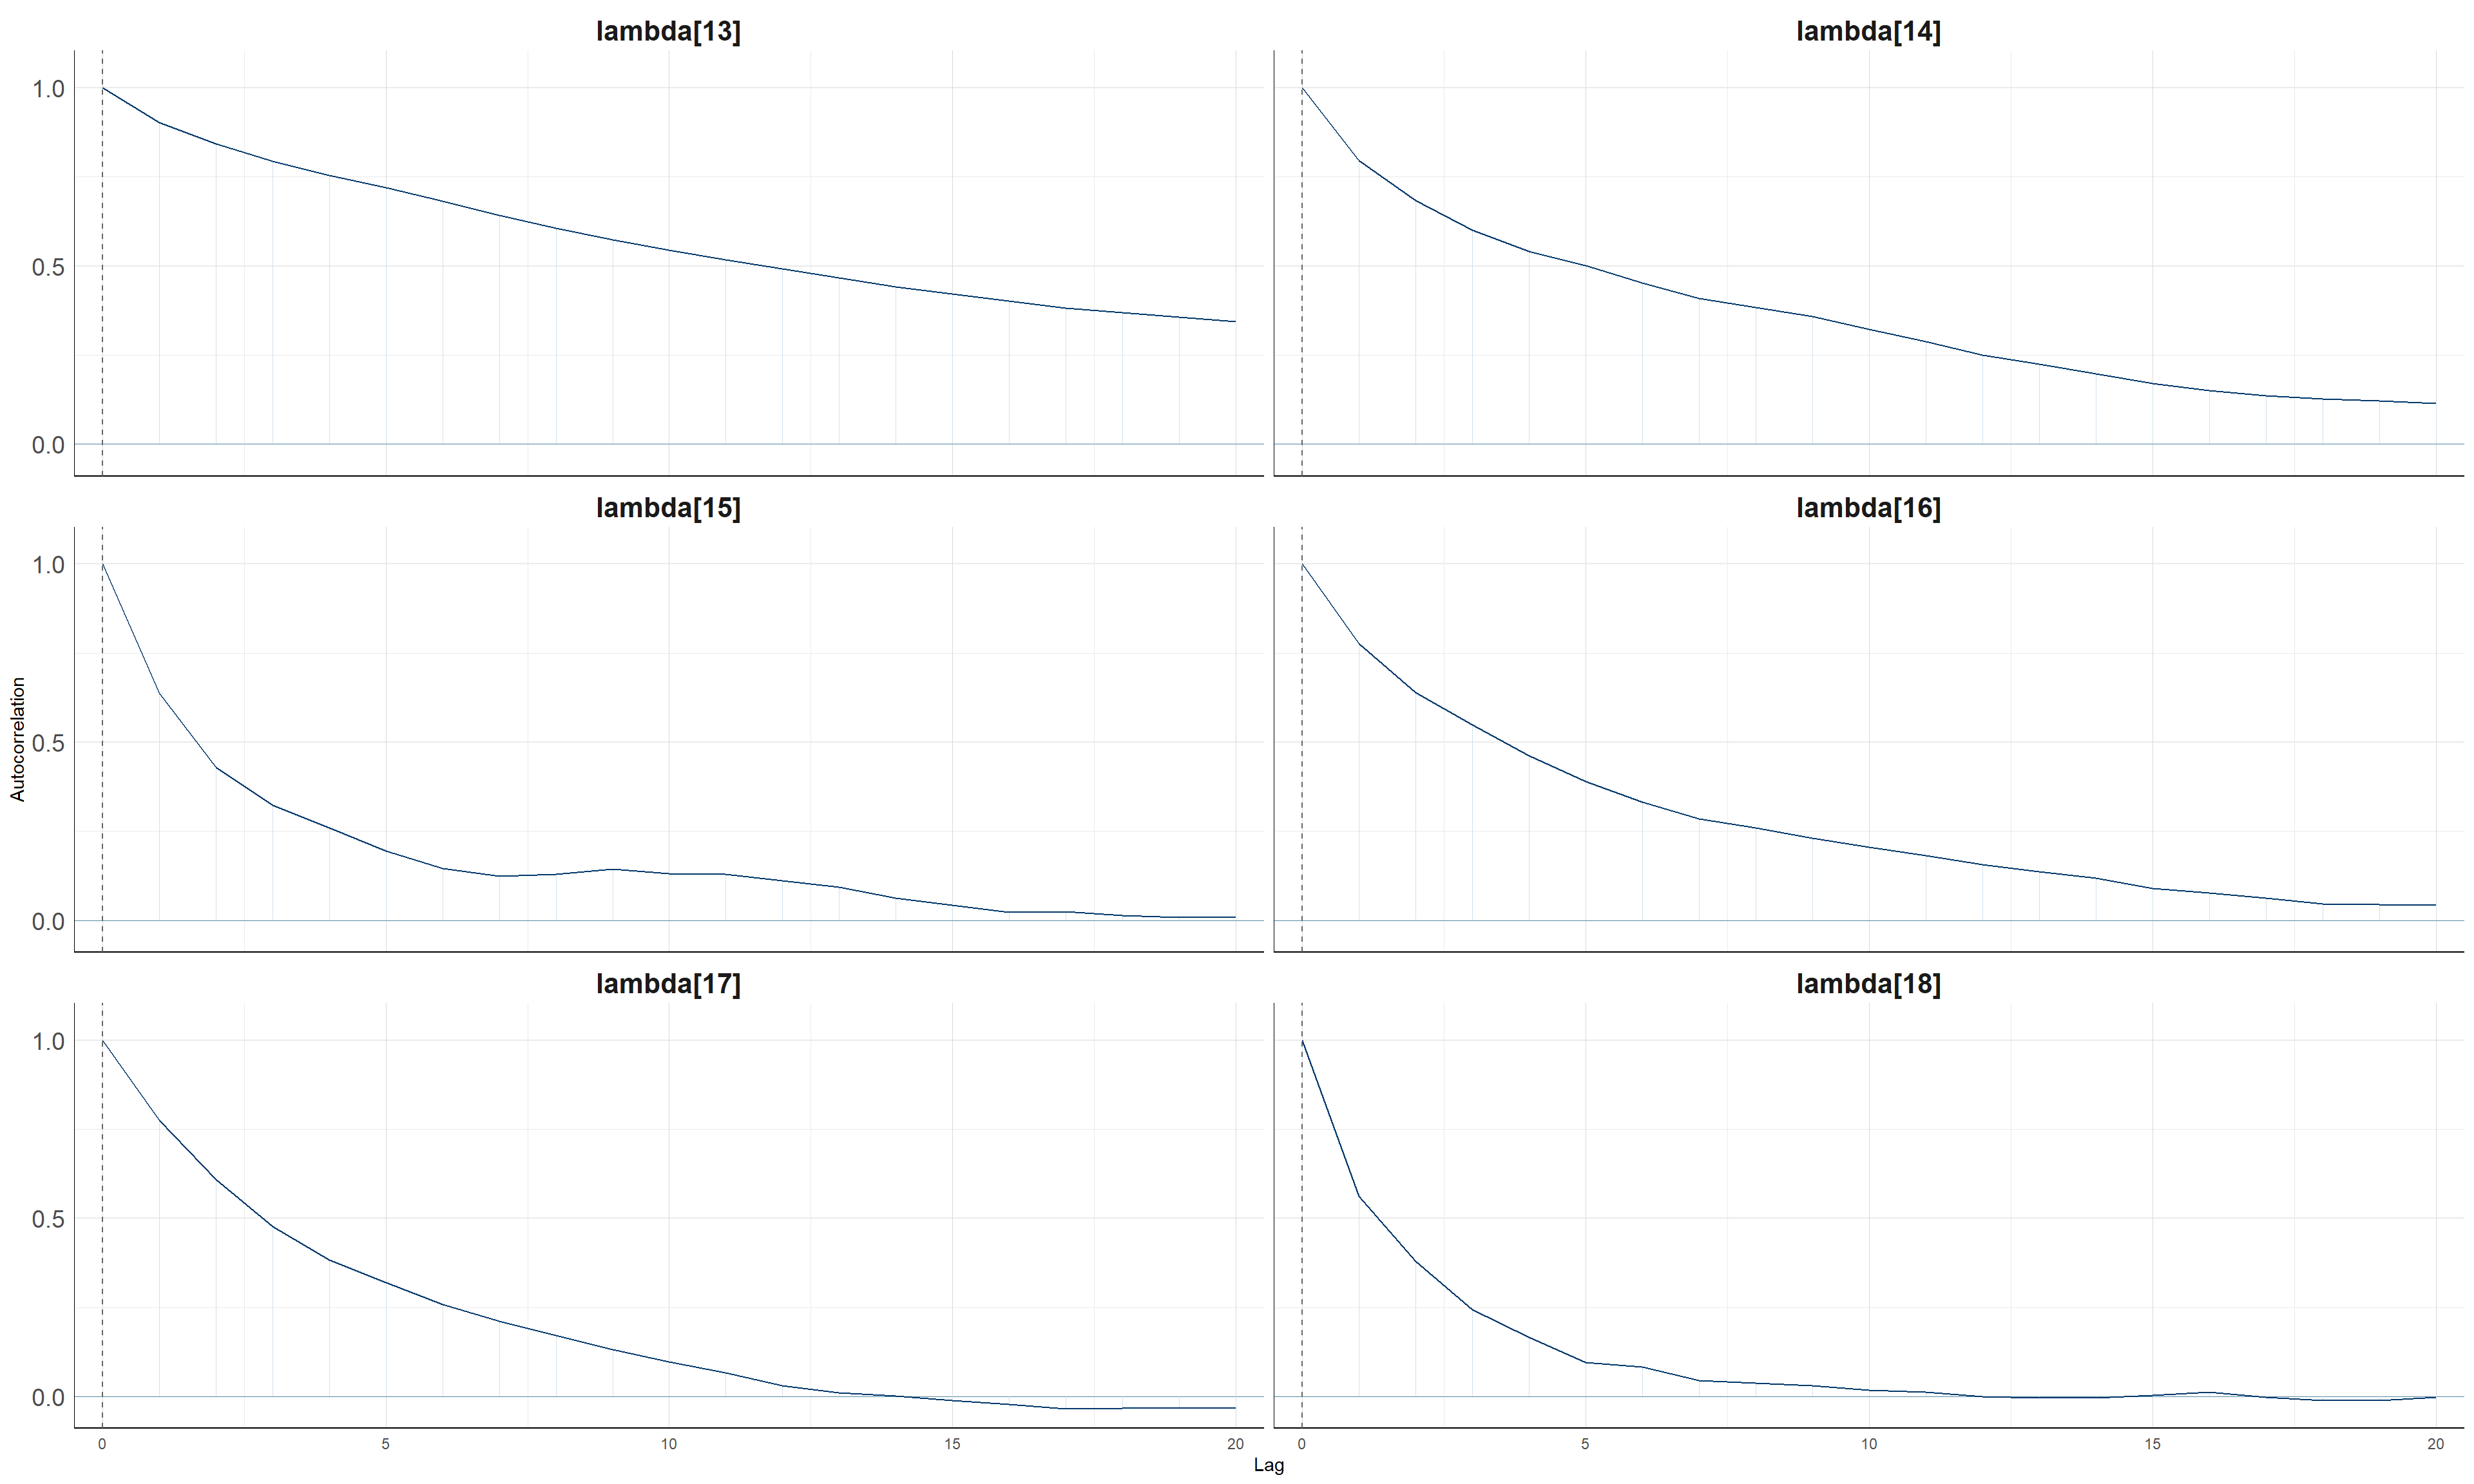
\includegraphics[width=\linewidth]{img/horseshoe_model/acf_lambda_chain1_3.png}
    \caption{Group 3.}
  \end{subfigure}\hfill
  \begin{subfigure}[t]{0.48\linewidth}
    \centering
    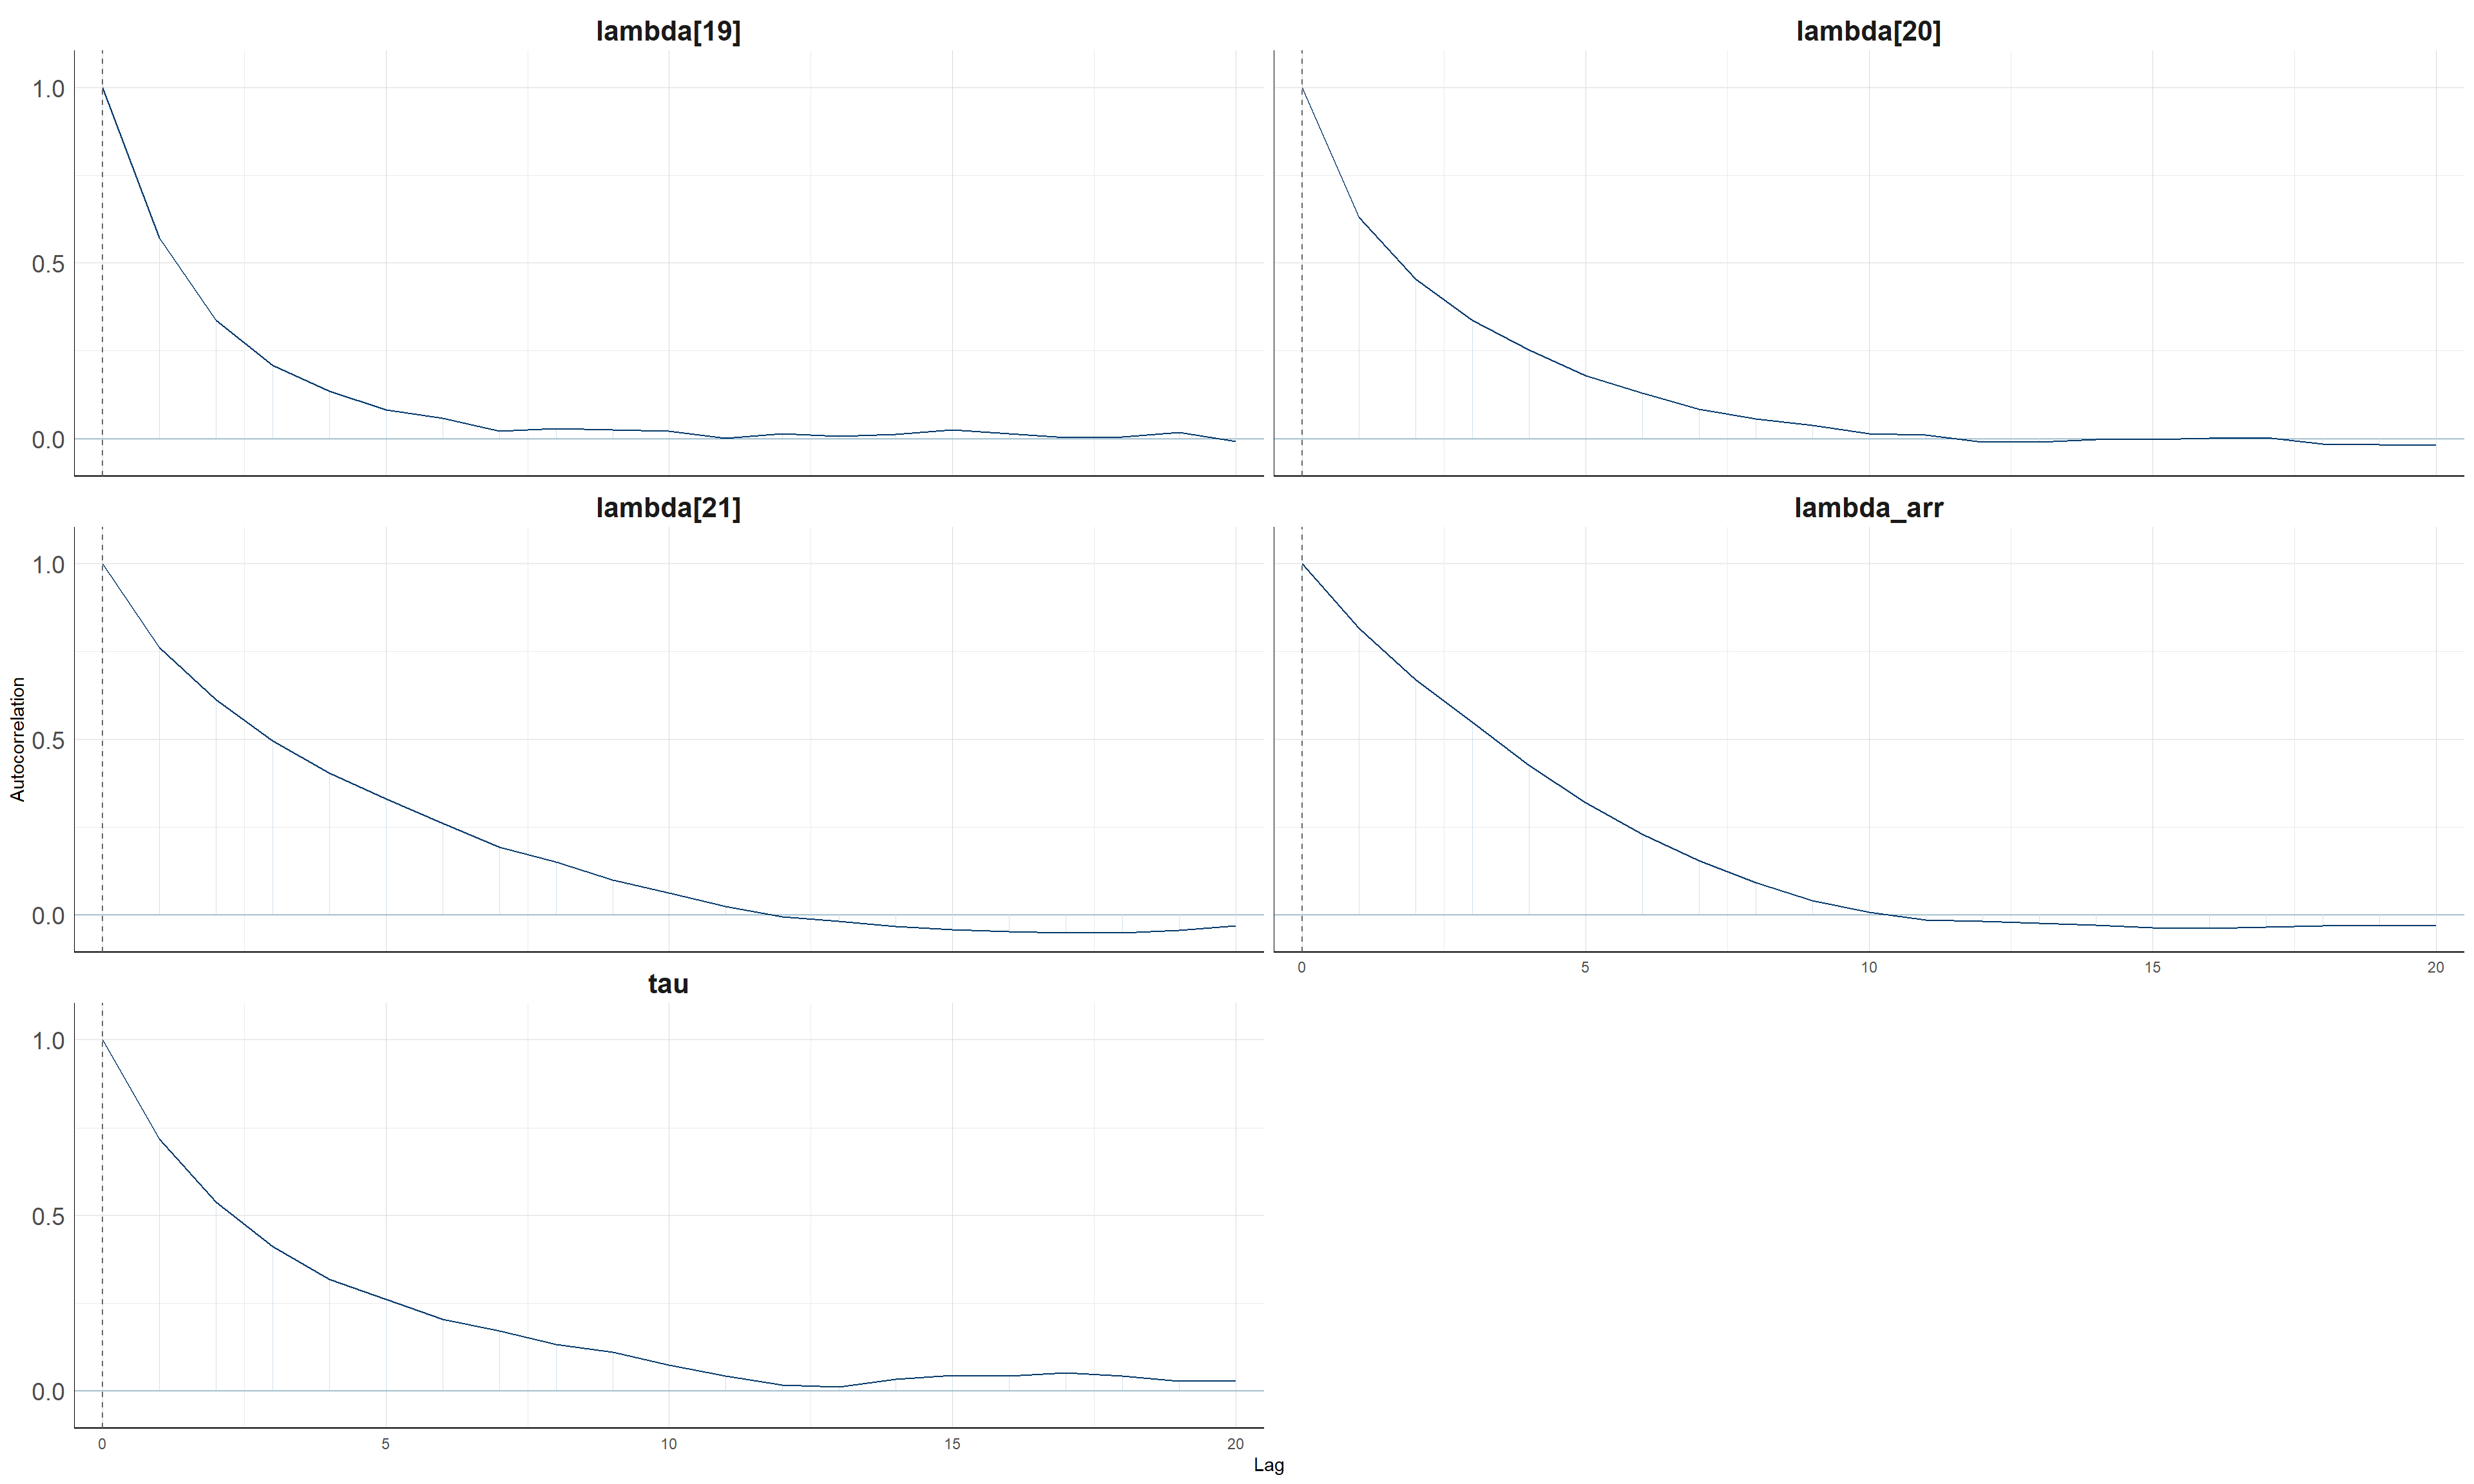
\includegraphics[width=\linewidth]{img/horseshoe_model/acf_lambda_chain1_4.png}
    \caption{Group 4.}
  \end{subfigure}\hfill
  \caption{Autocorrelation of the scales $\lambda_j$, chain 1.}
  \label{fig:hs_acf_lambda_1}
\end{figure}

\begin{figure}[htbp]
  \centering
  \begin{subfigure}[t]{0.48\linewidth}
    \centering
    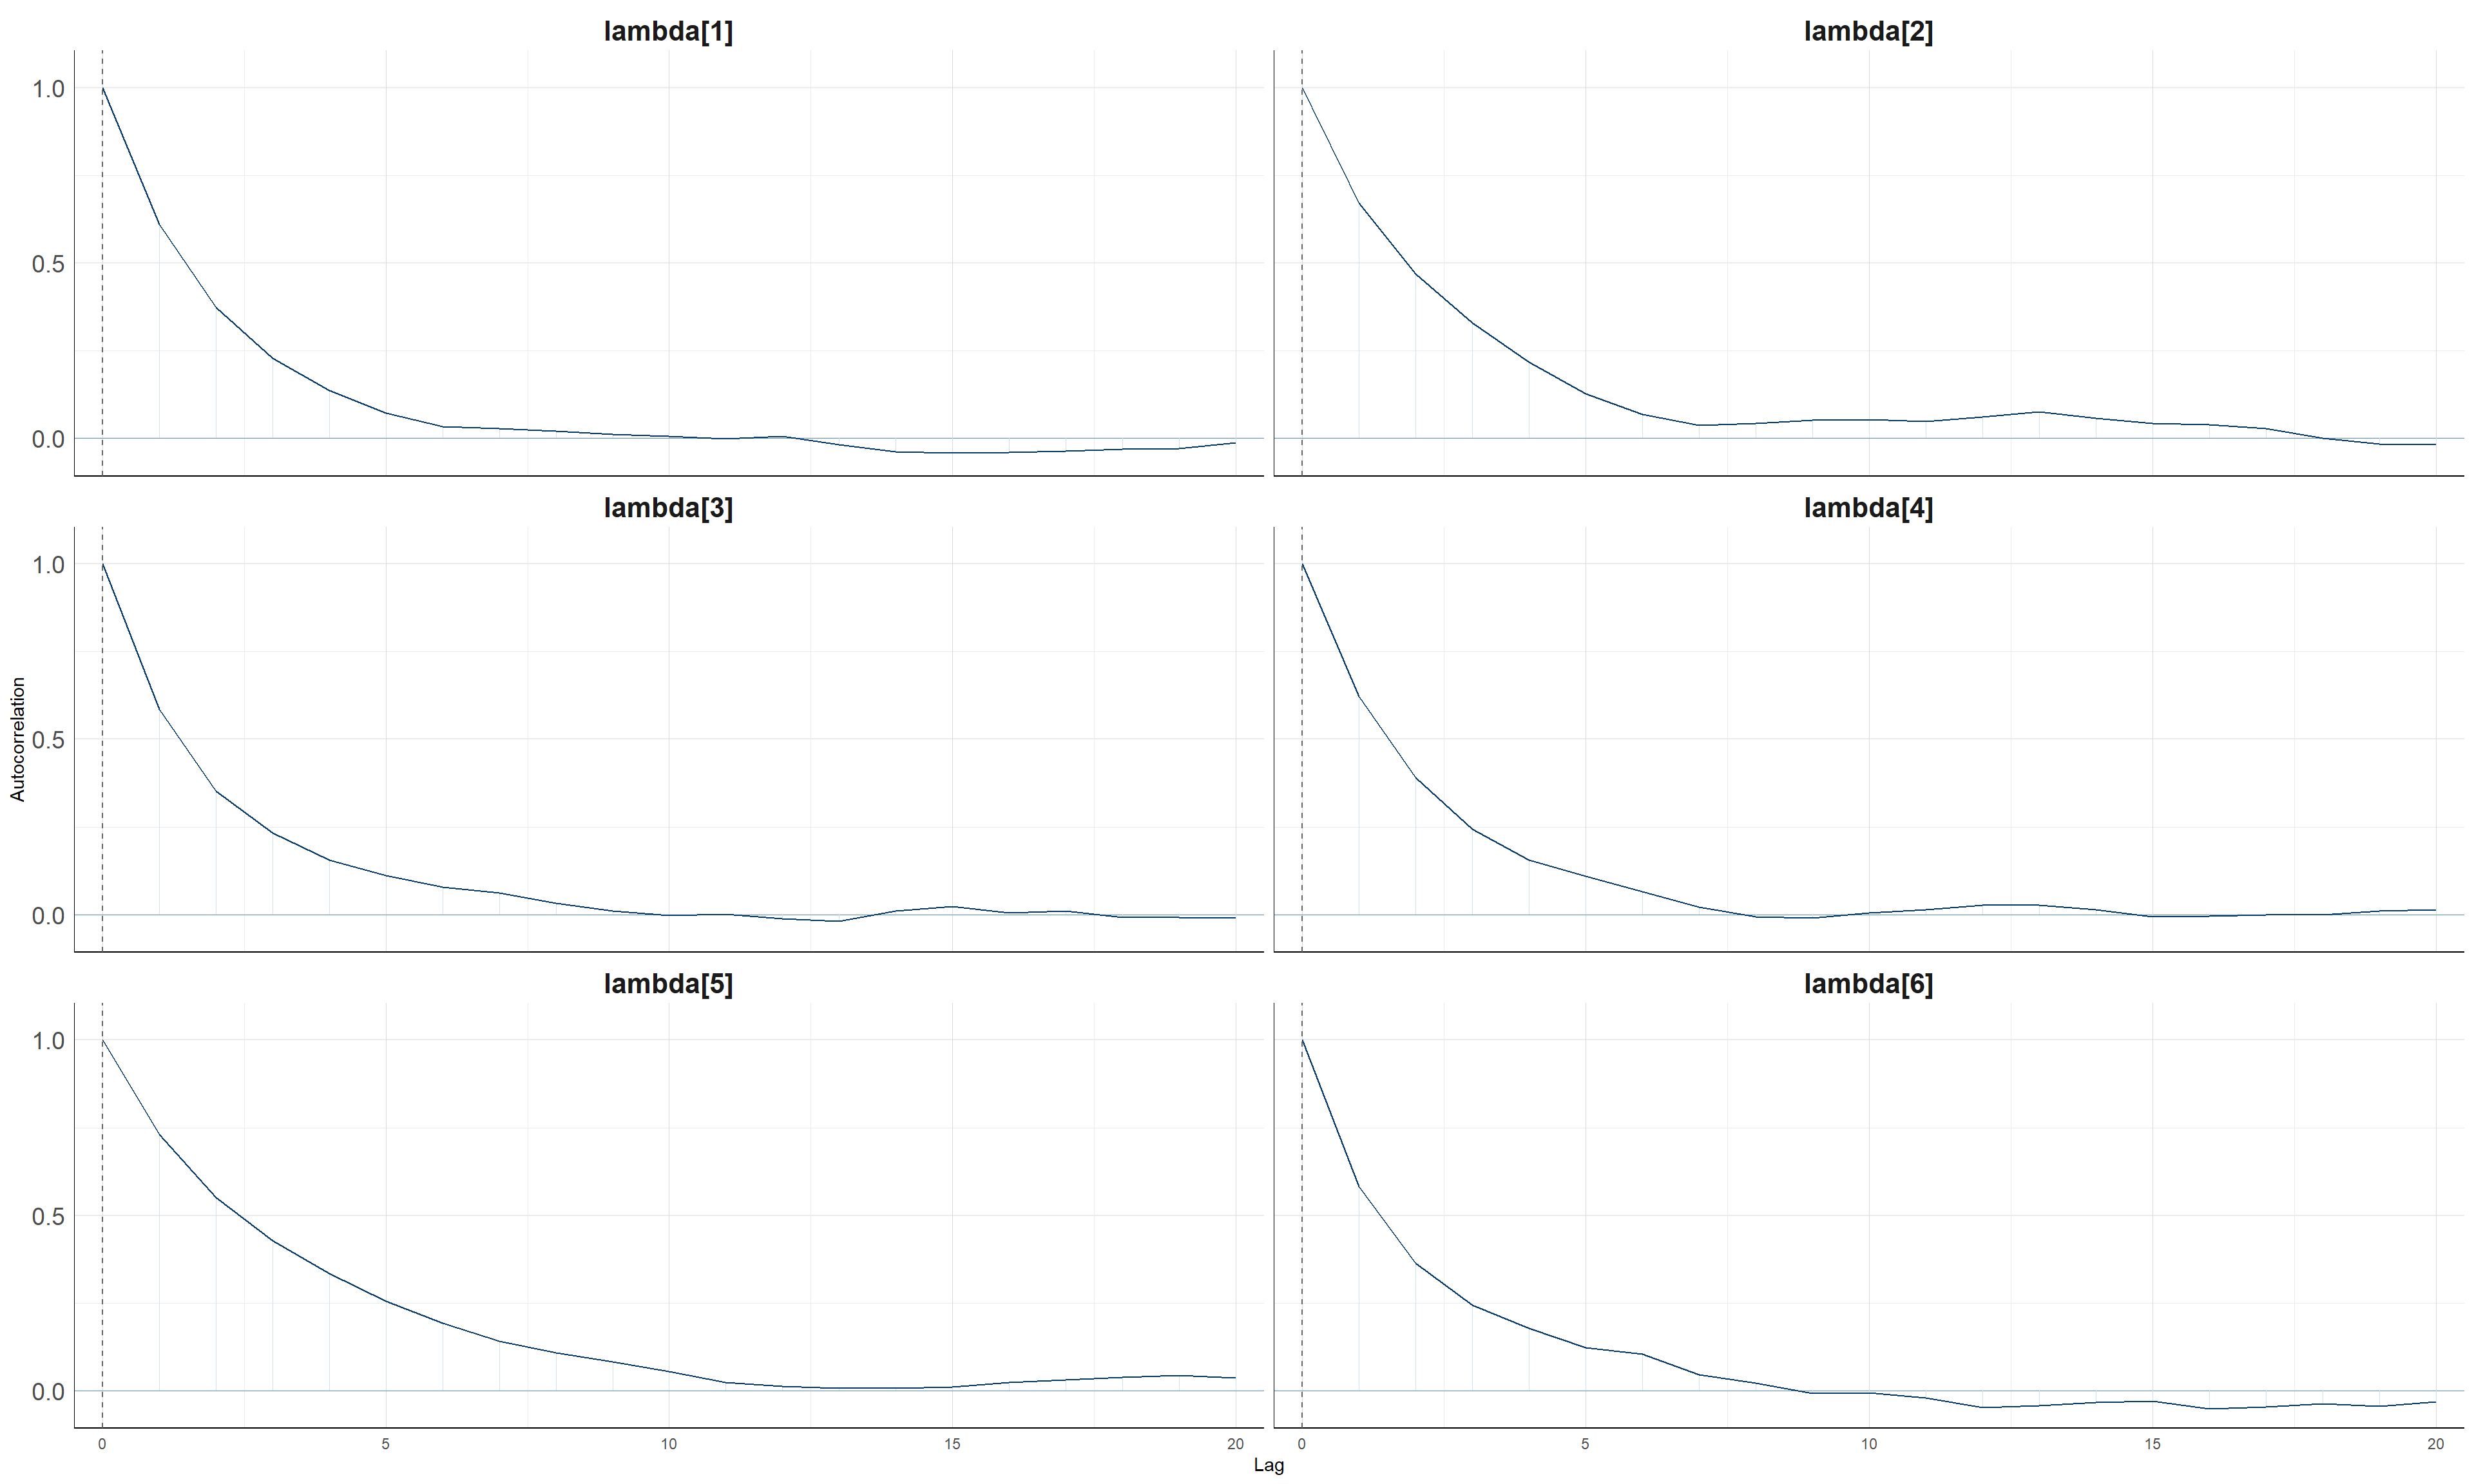
\includegraphics[width=\linewidth]{img/horseshoe_model/acf_lambda_chain2_1.png}
    \caption{Group 1.}
  \end{subfigure}\hfill
  \begin{subfigure}[t]{0.48\linewidth}
    \centering
    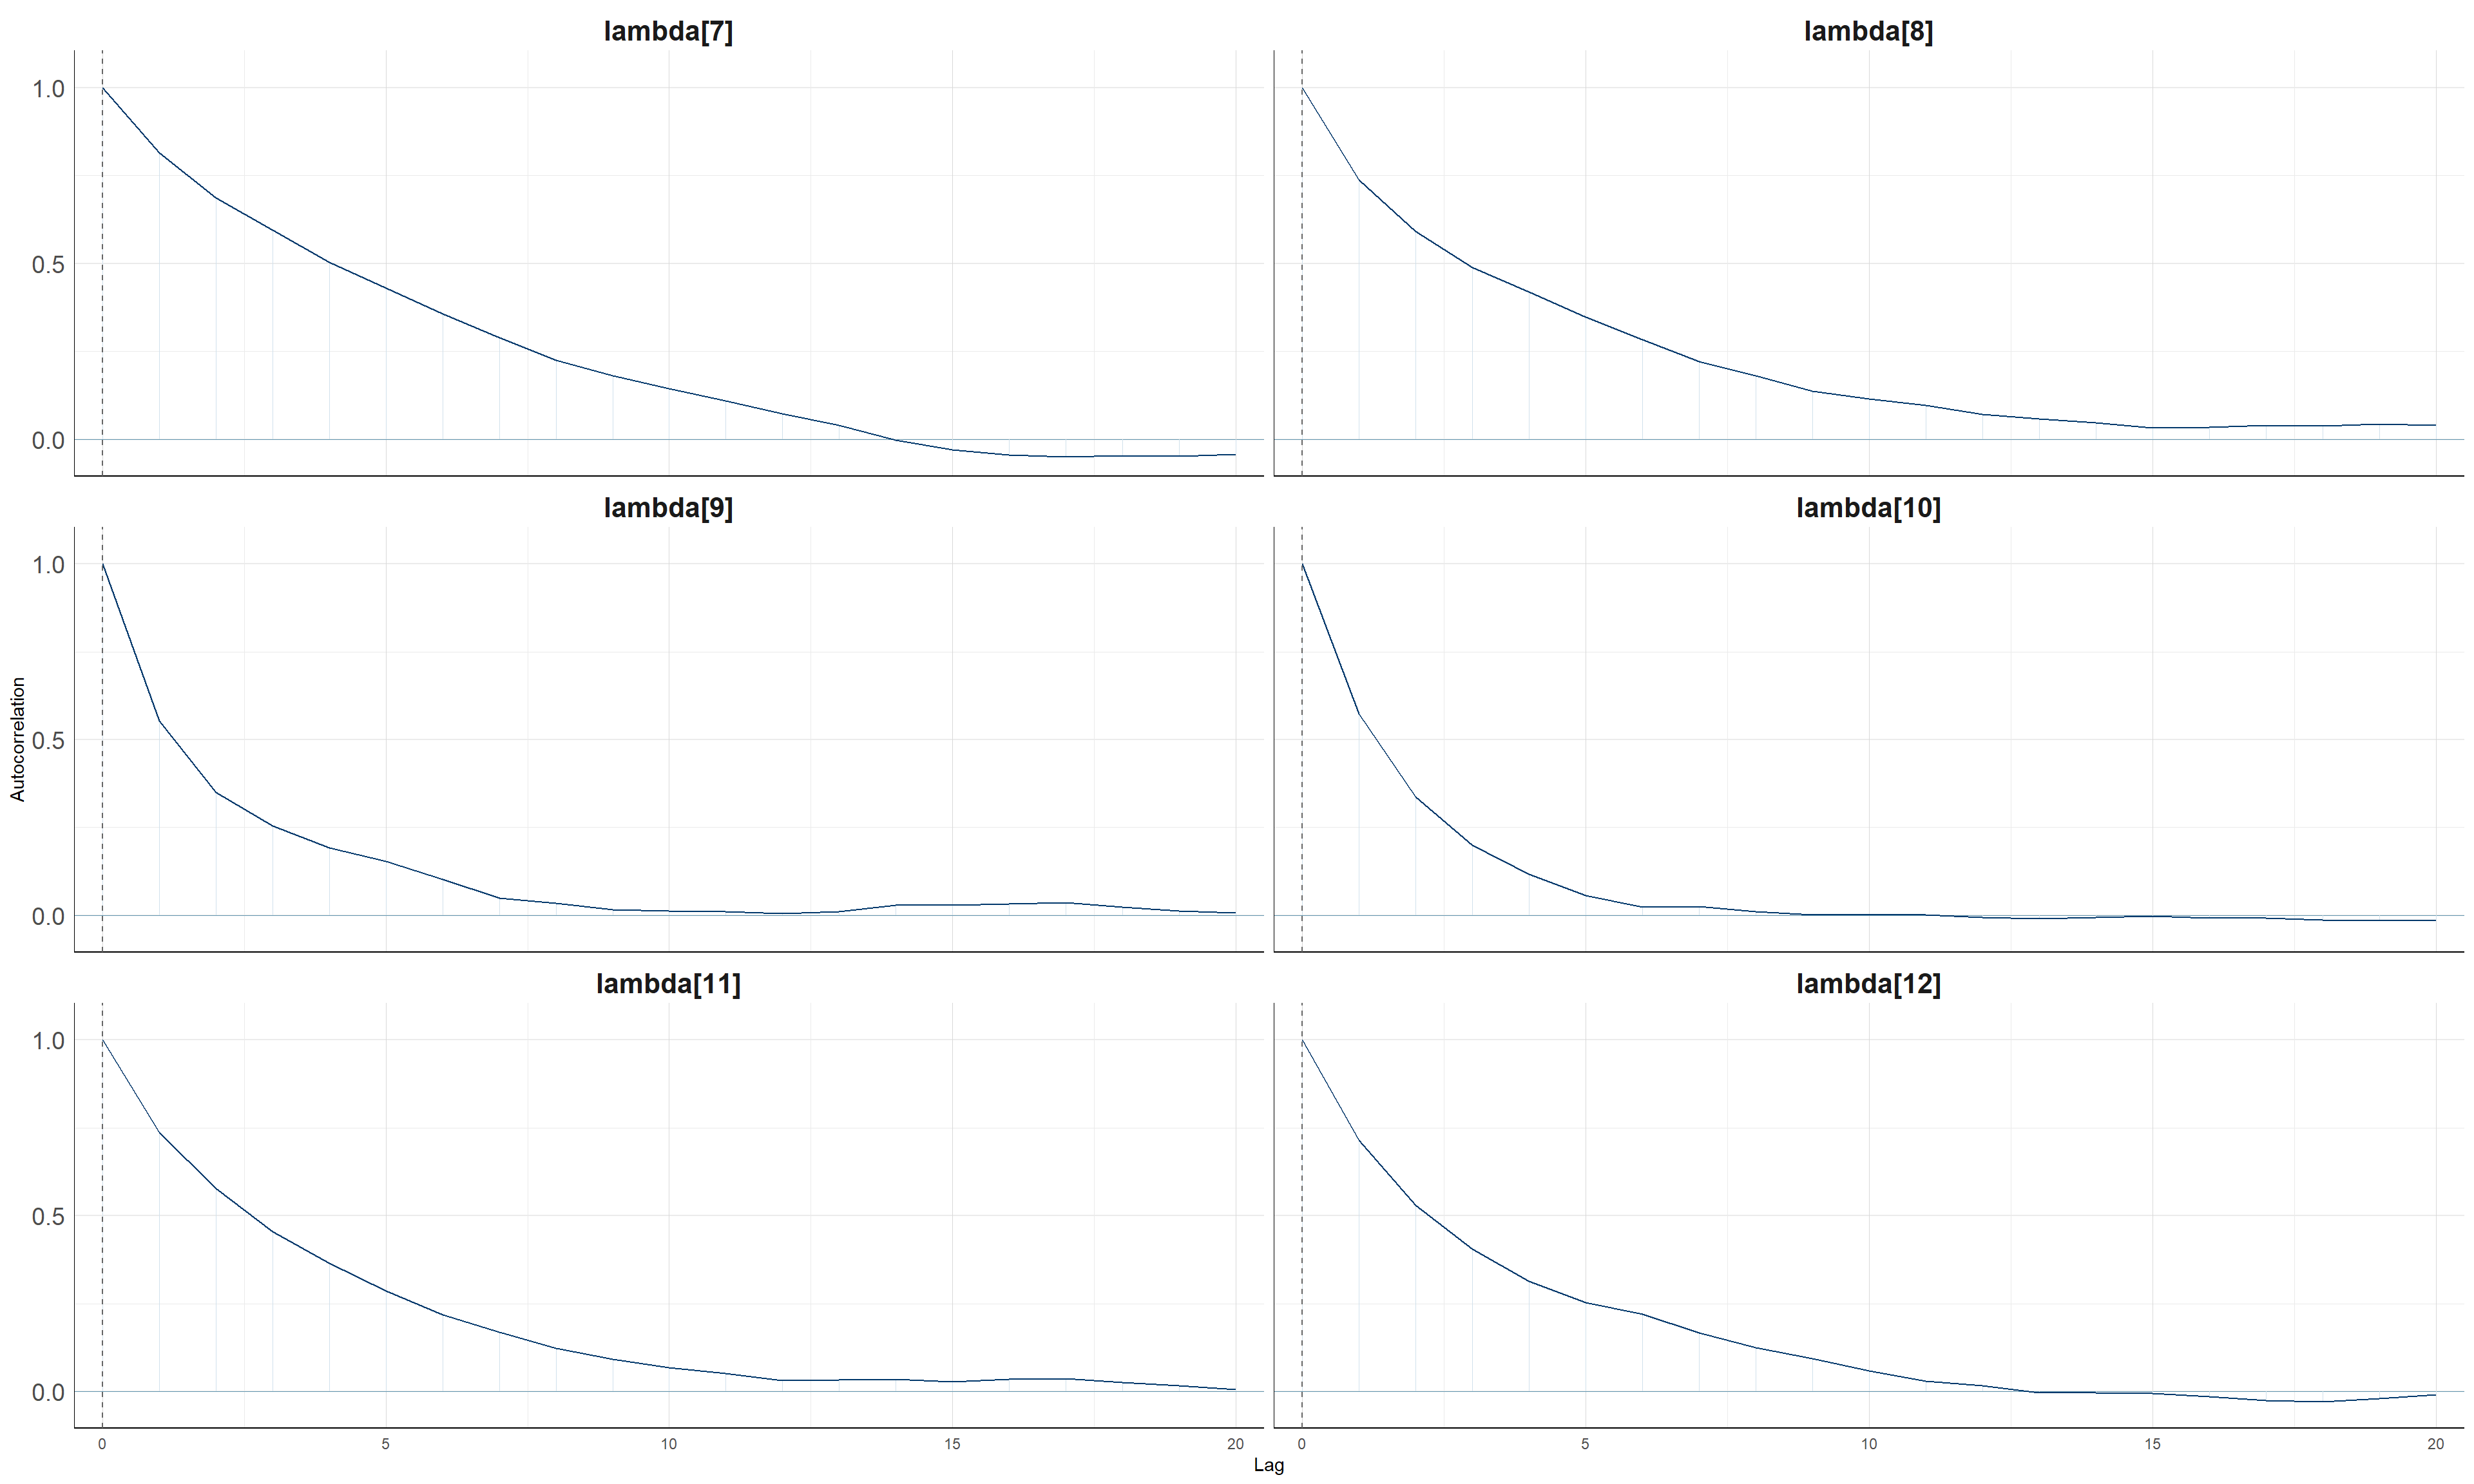
\includegraphics[width=\linewidth]{img/horseshoe_model/acf_lambda_chain2_2.png}
    \caption{Group 2.}
  \end{subfigure}\hfill
  \begin{subfigure}[t]{0.48\linewidth}
    \centering
    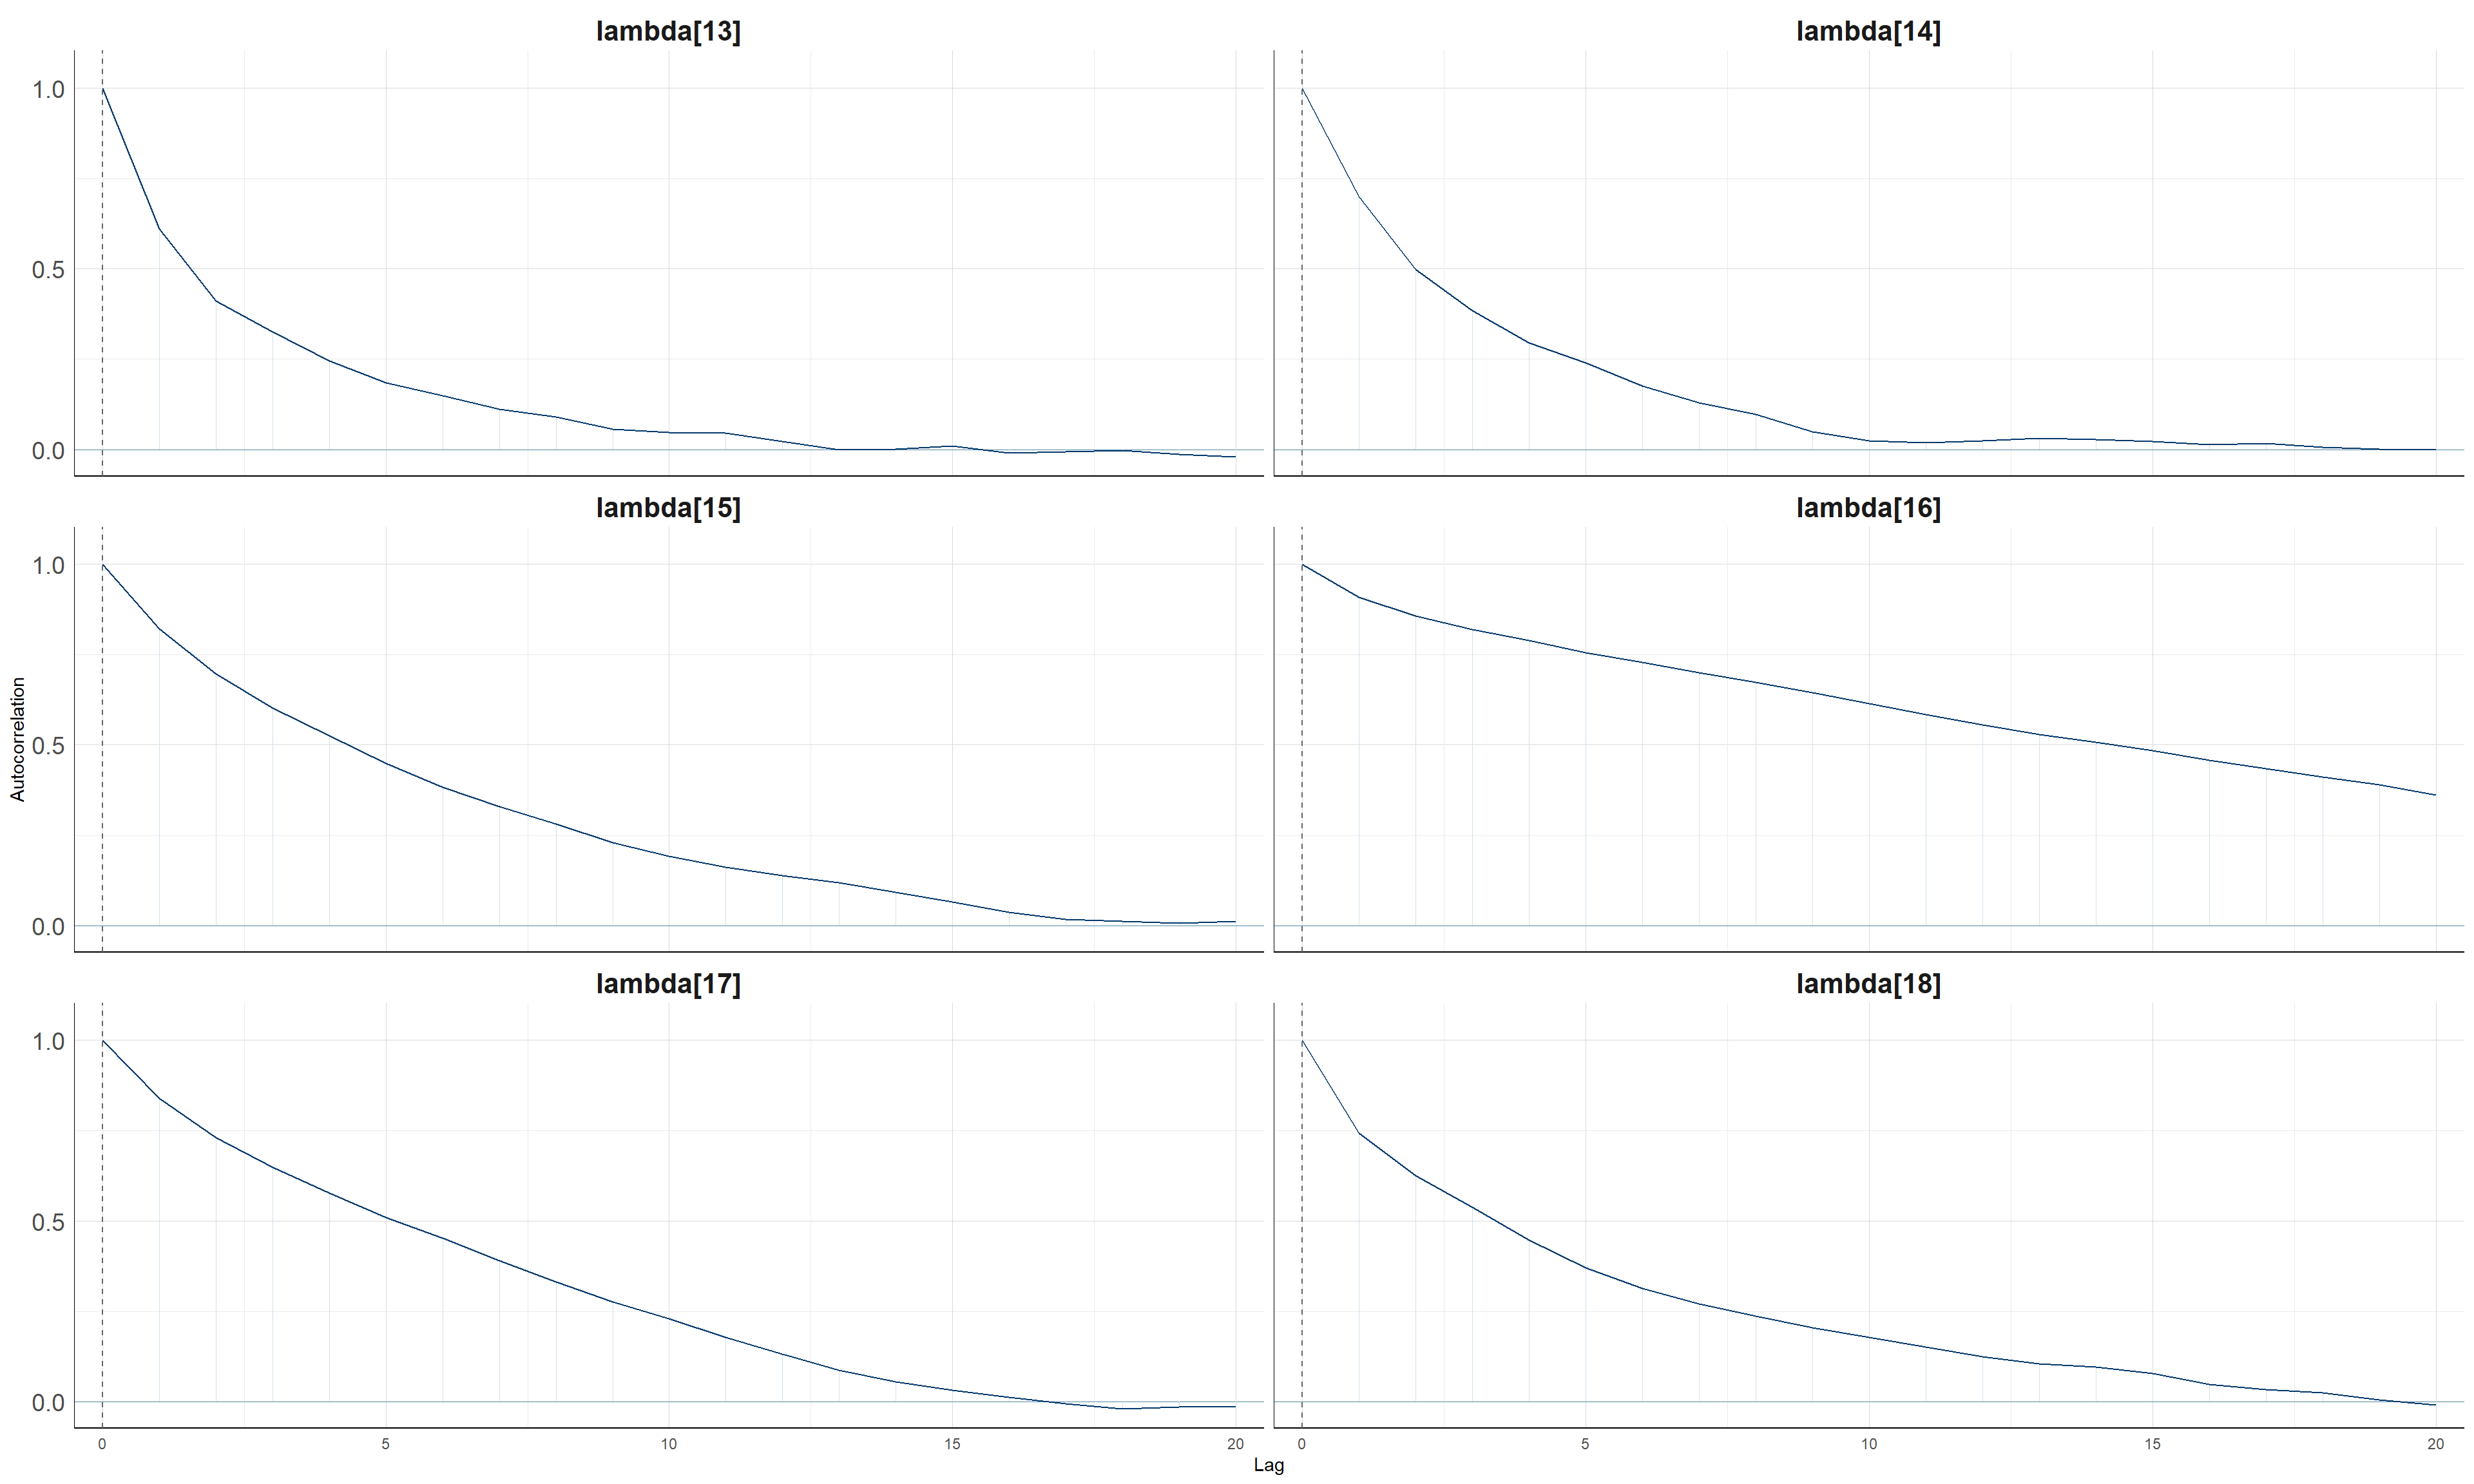
\includegraphics[width=\linewidth]{img/horseshoe_model/acf_lambda_chain2_3.png}
    \caption{Group 3.}
  \end{subfigure}\hfill
  \begin{subfigure}[t]{0.48\linewidth}
    \centering
    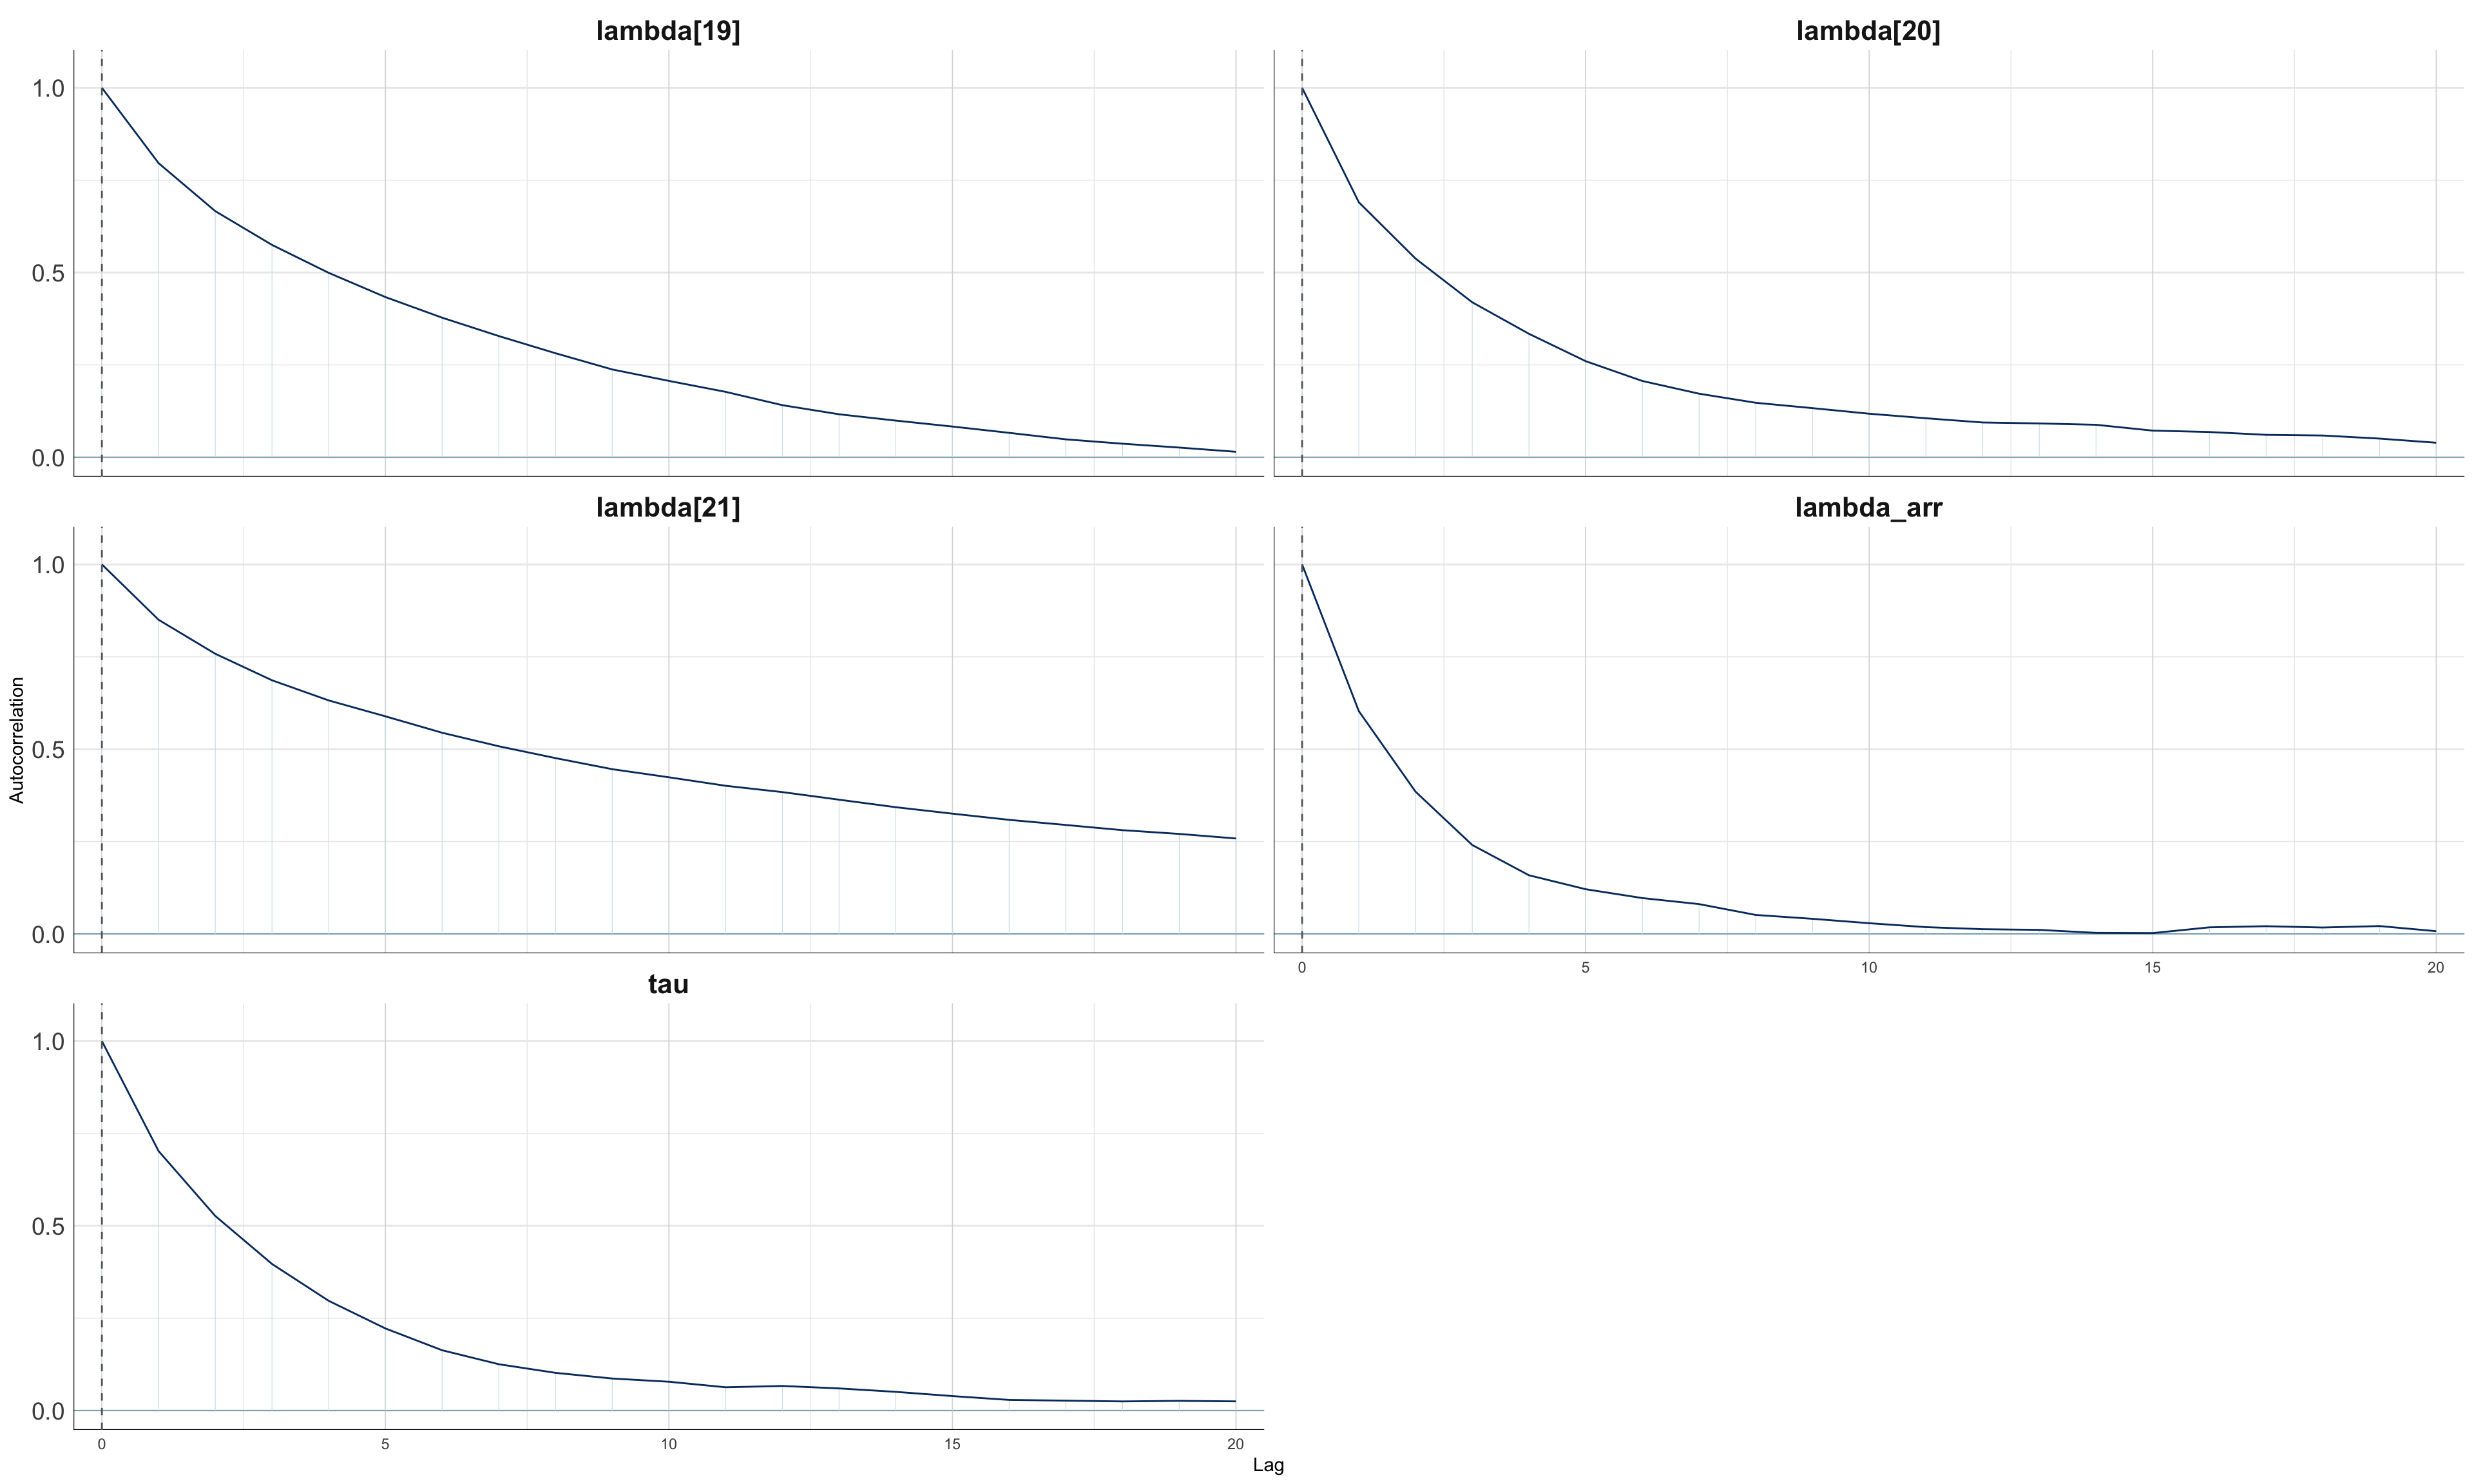
\includegraphics[width=\linewidth]{img/horseshoe_model/acf_lambda_chain2_4.png}
    \caption{Group 4.}
  \end{subfigure}\hfill
  \caption{Autocorrelation of the scales $\lambda_j$, chain 2.}
  \label{fig:hs_acf_lambda_2}
\end{figure}

\begin{figure}[htbp]
  \centering
  \begin{subfigure}[t]{0.48\linewidth}
    \centering
    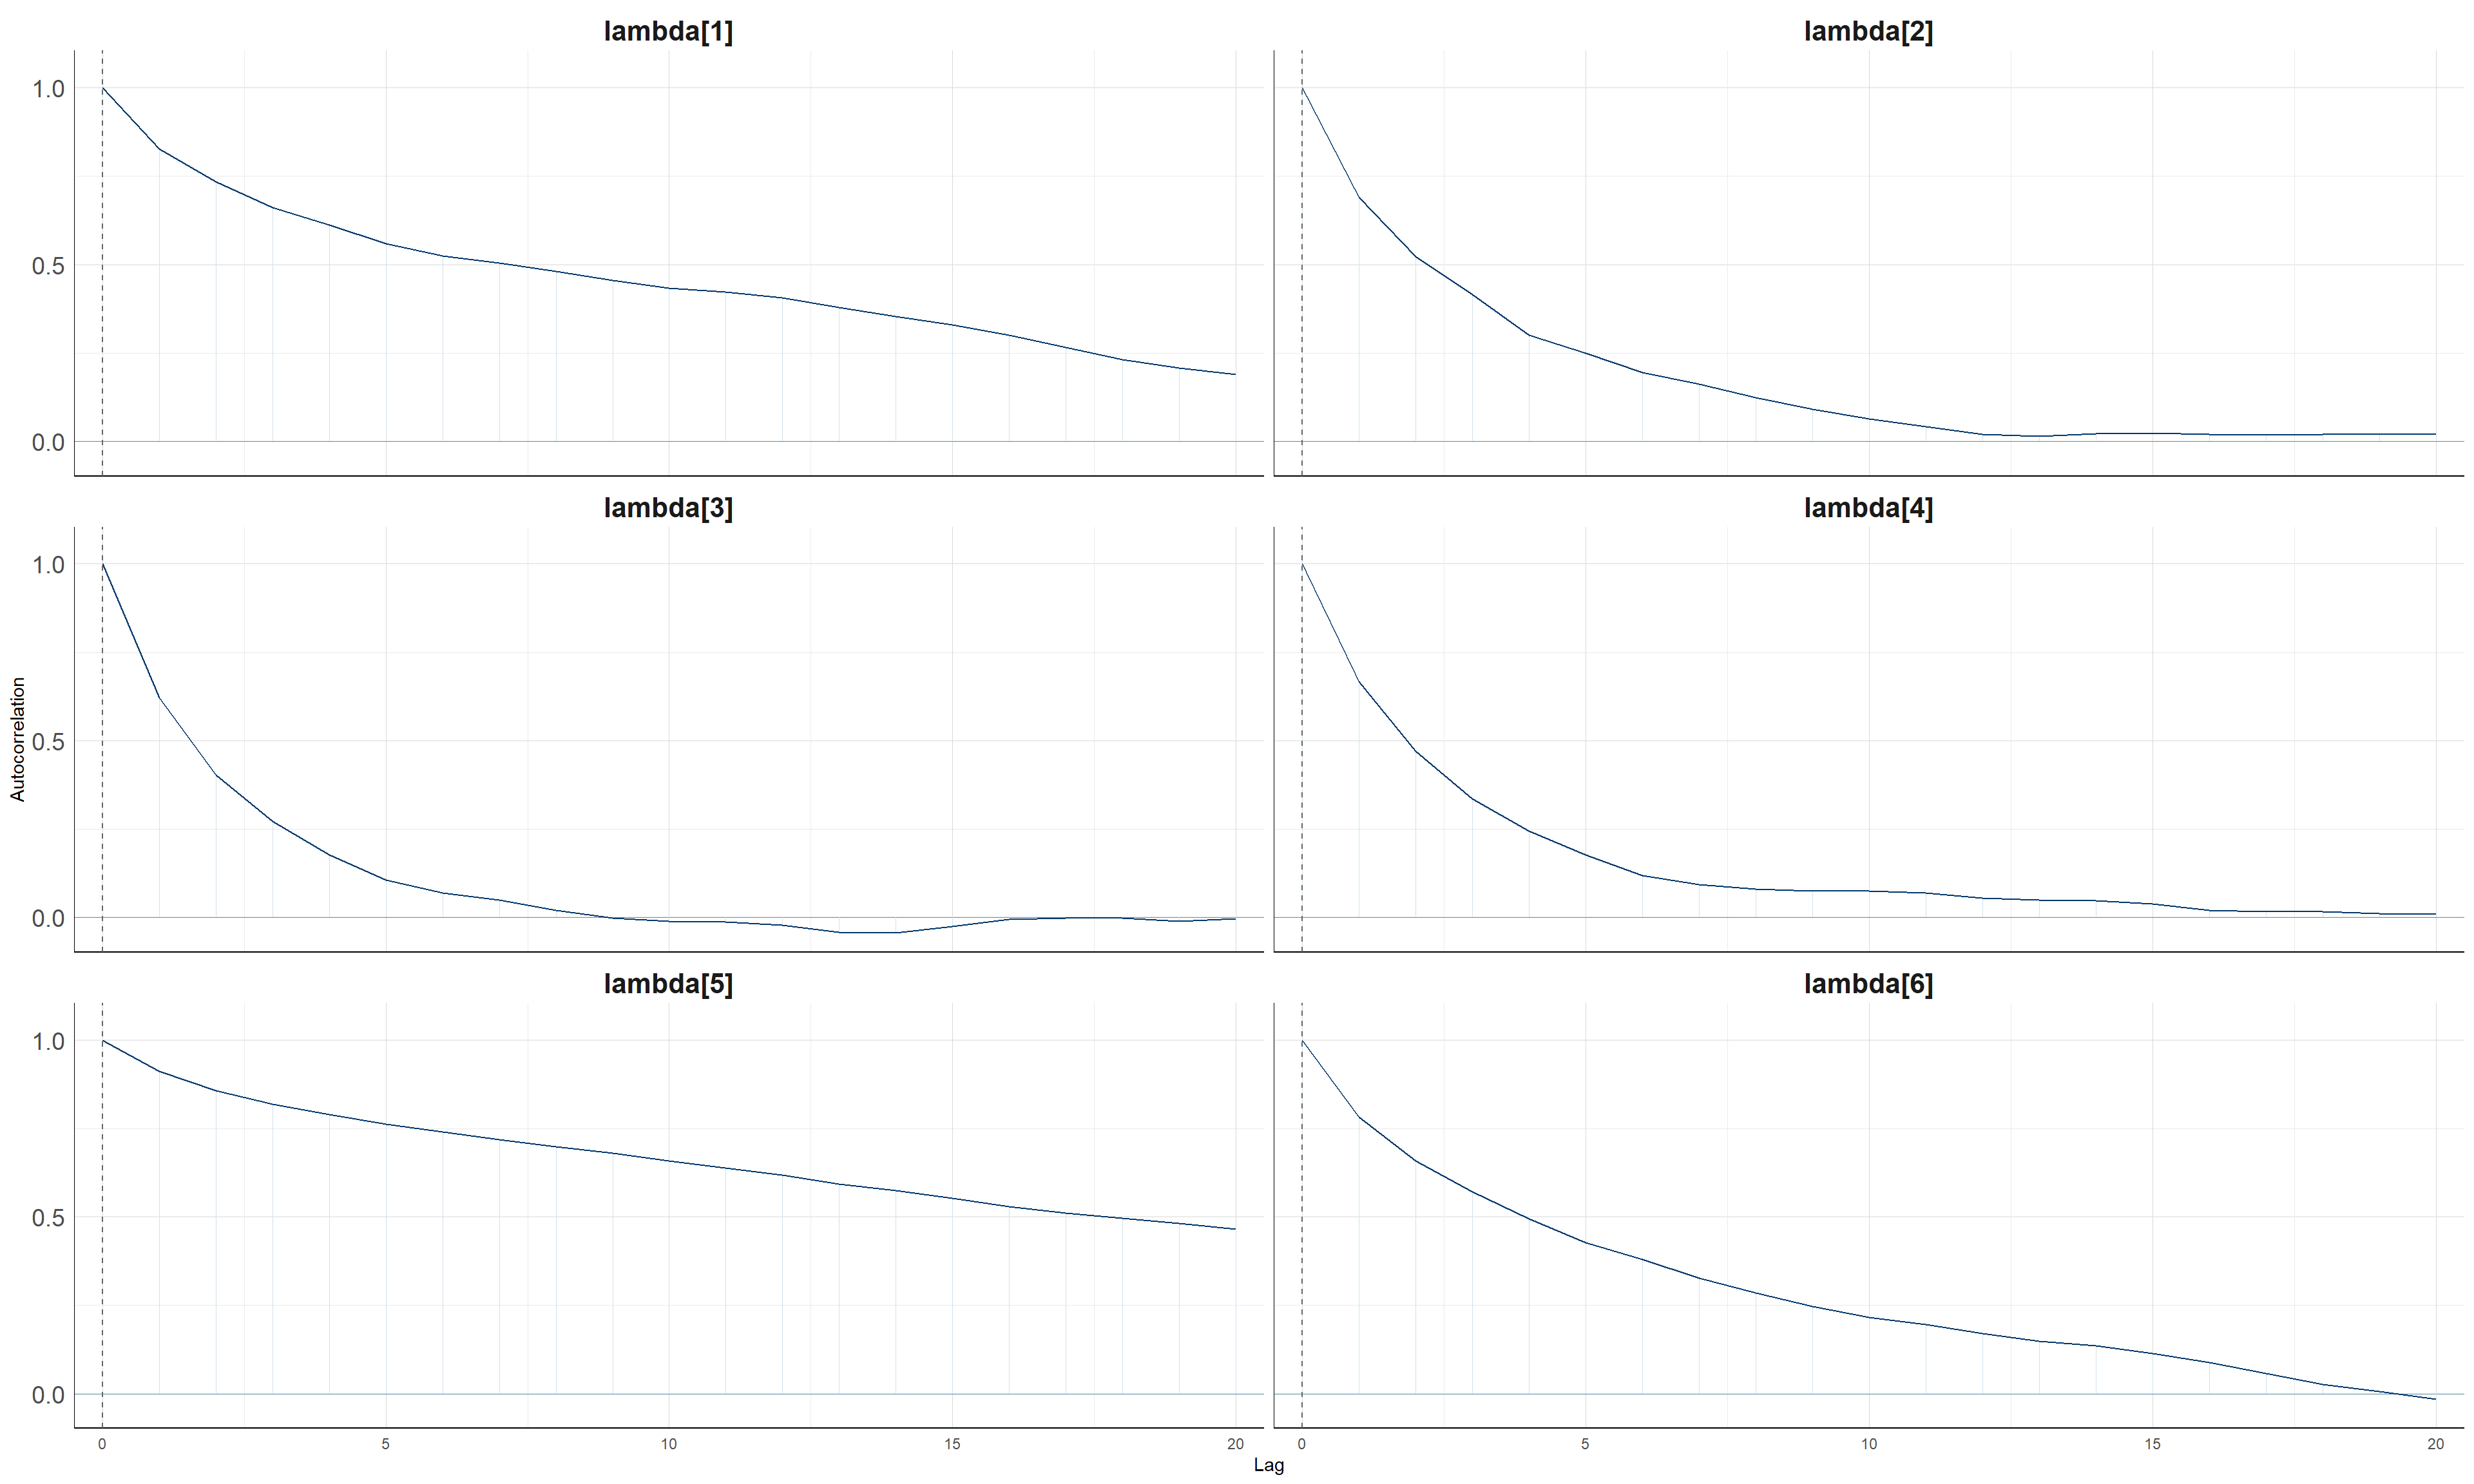
\includegraphics[width=\linewidth]{img/horseshoe_model/acf_lambda_chain3_1.png}
    \caption{Group 1.}
  \end{subfigure}\hfill
  \begin{subfigure}[t]{0.48\linewidth}
    \centering
    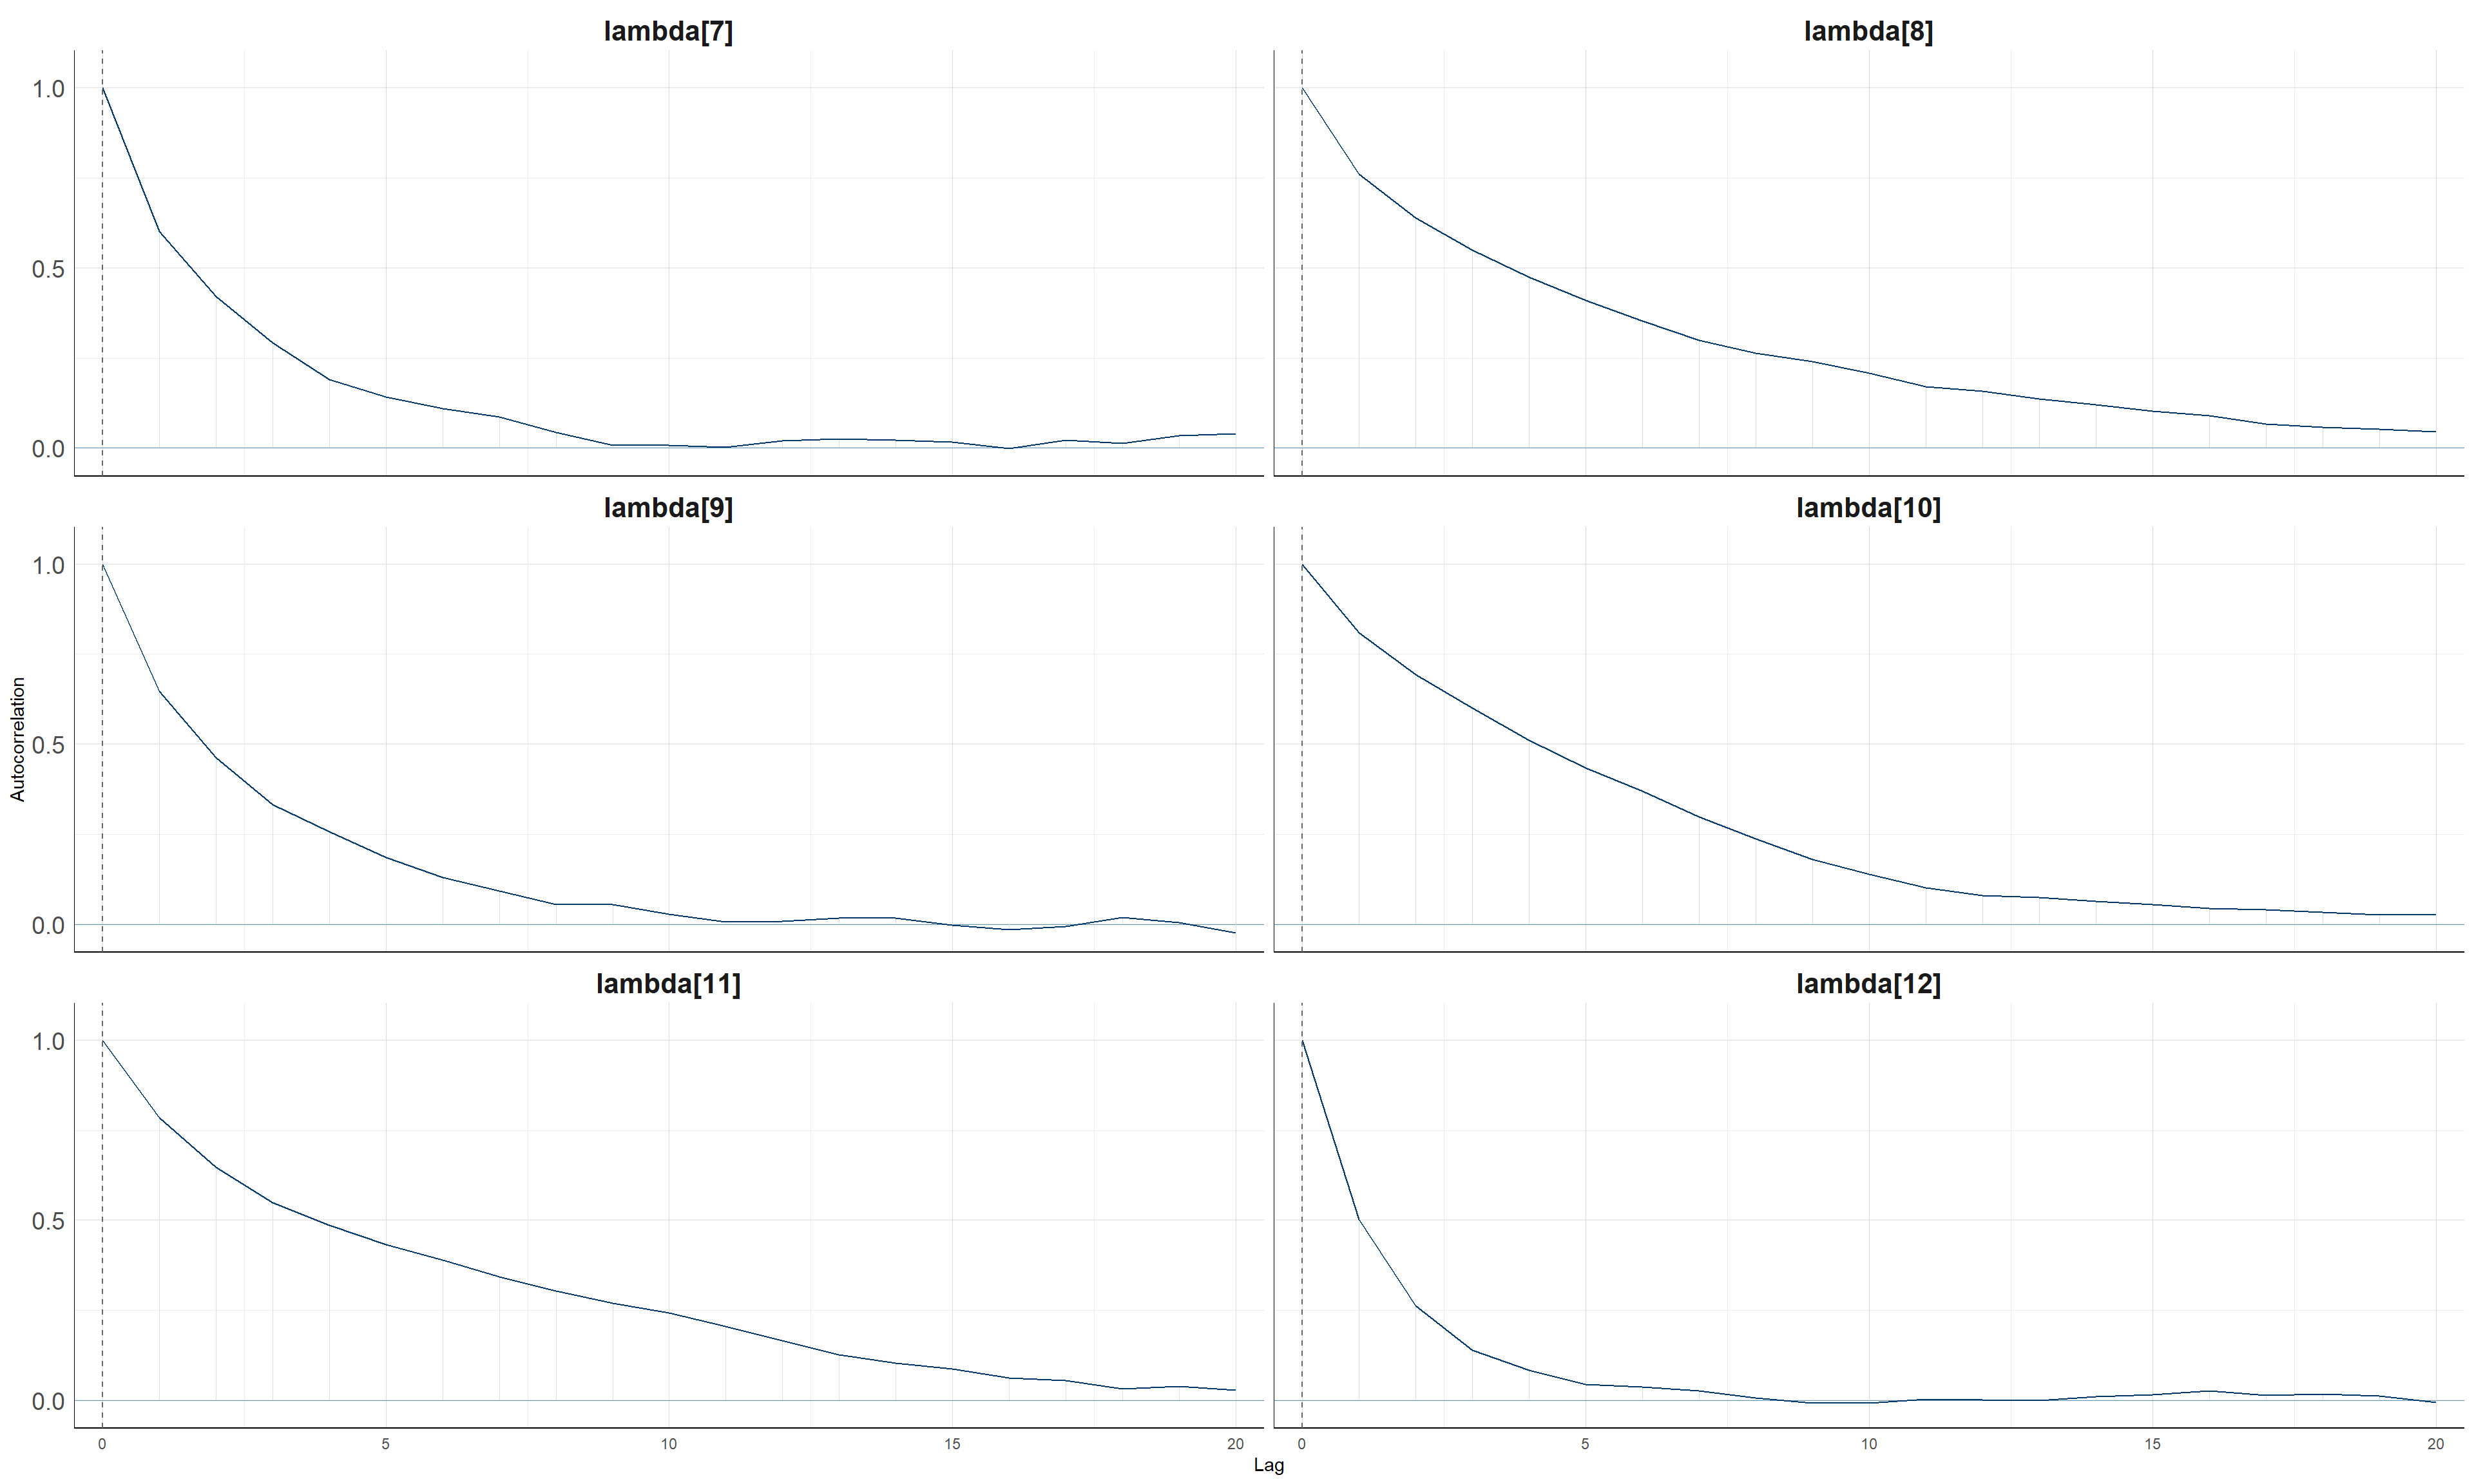
\includegraphics[width=\linewidth]{img/horseshoe_model/acf_lambda_chain3_2.png}
    \caption{Group 2.}
  \end{subfigure}\hfill
  \begin{subfigure}[t]{0.48\linewidth}
    \centering
    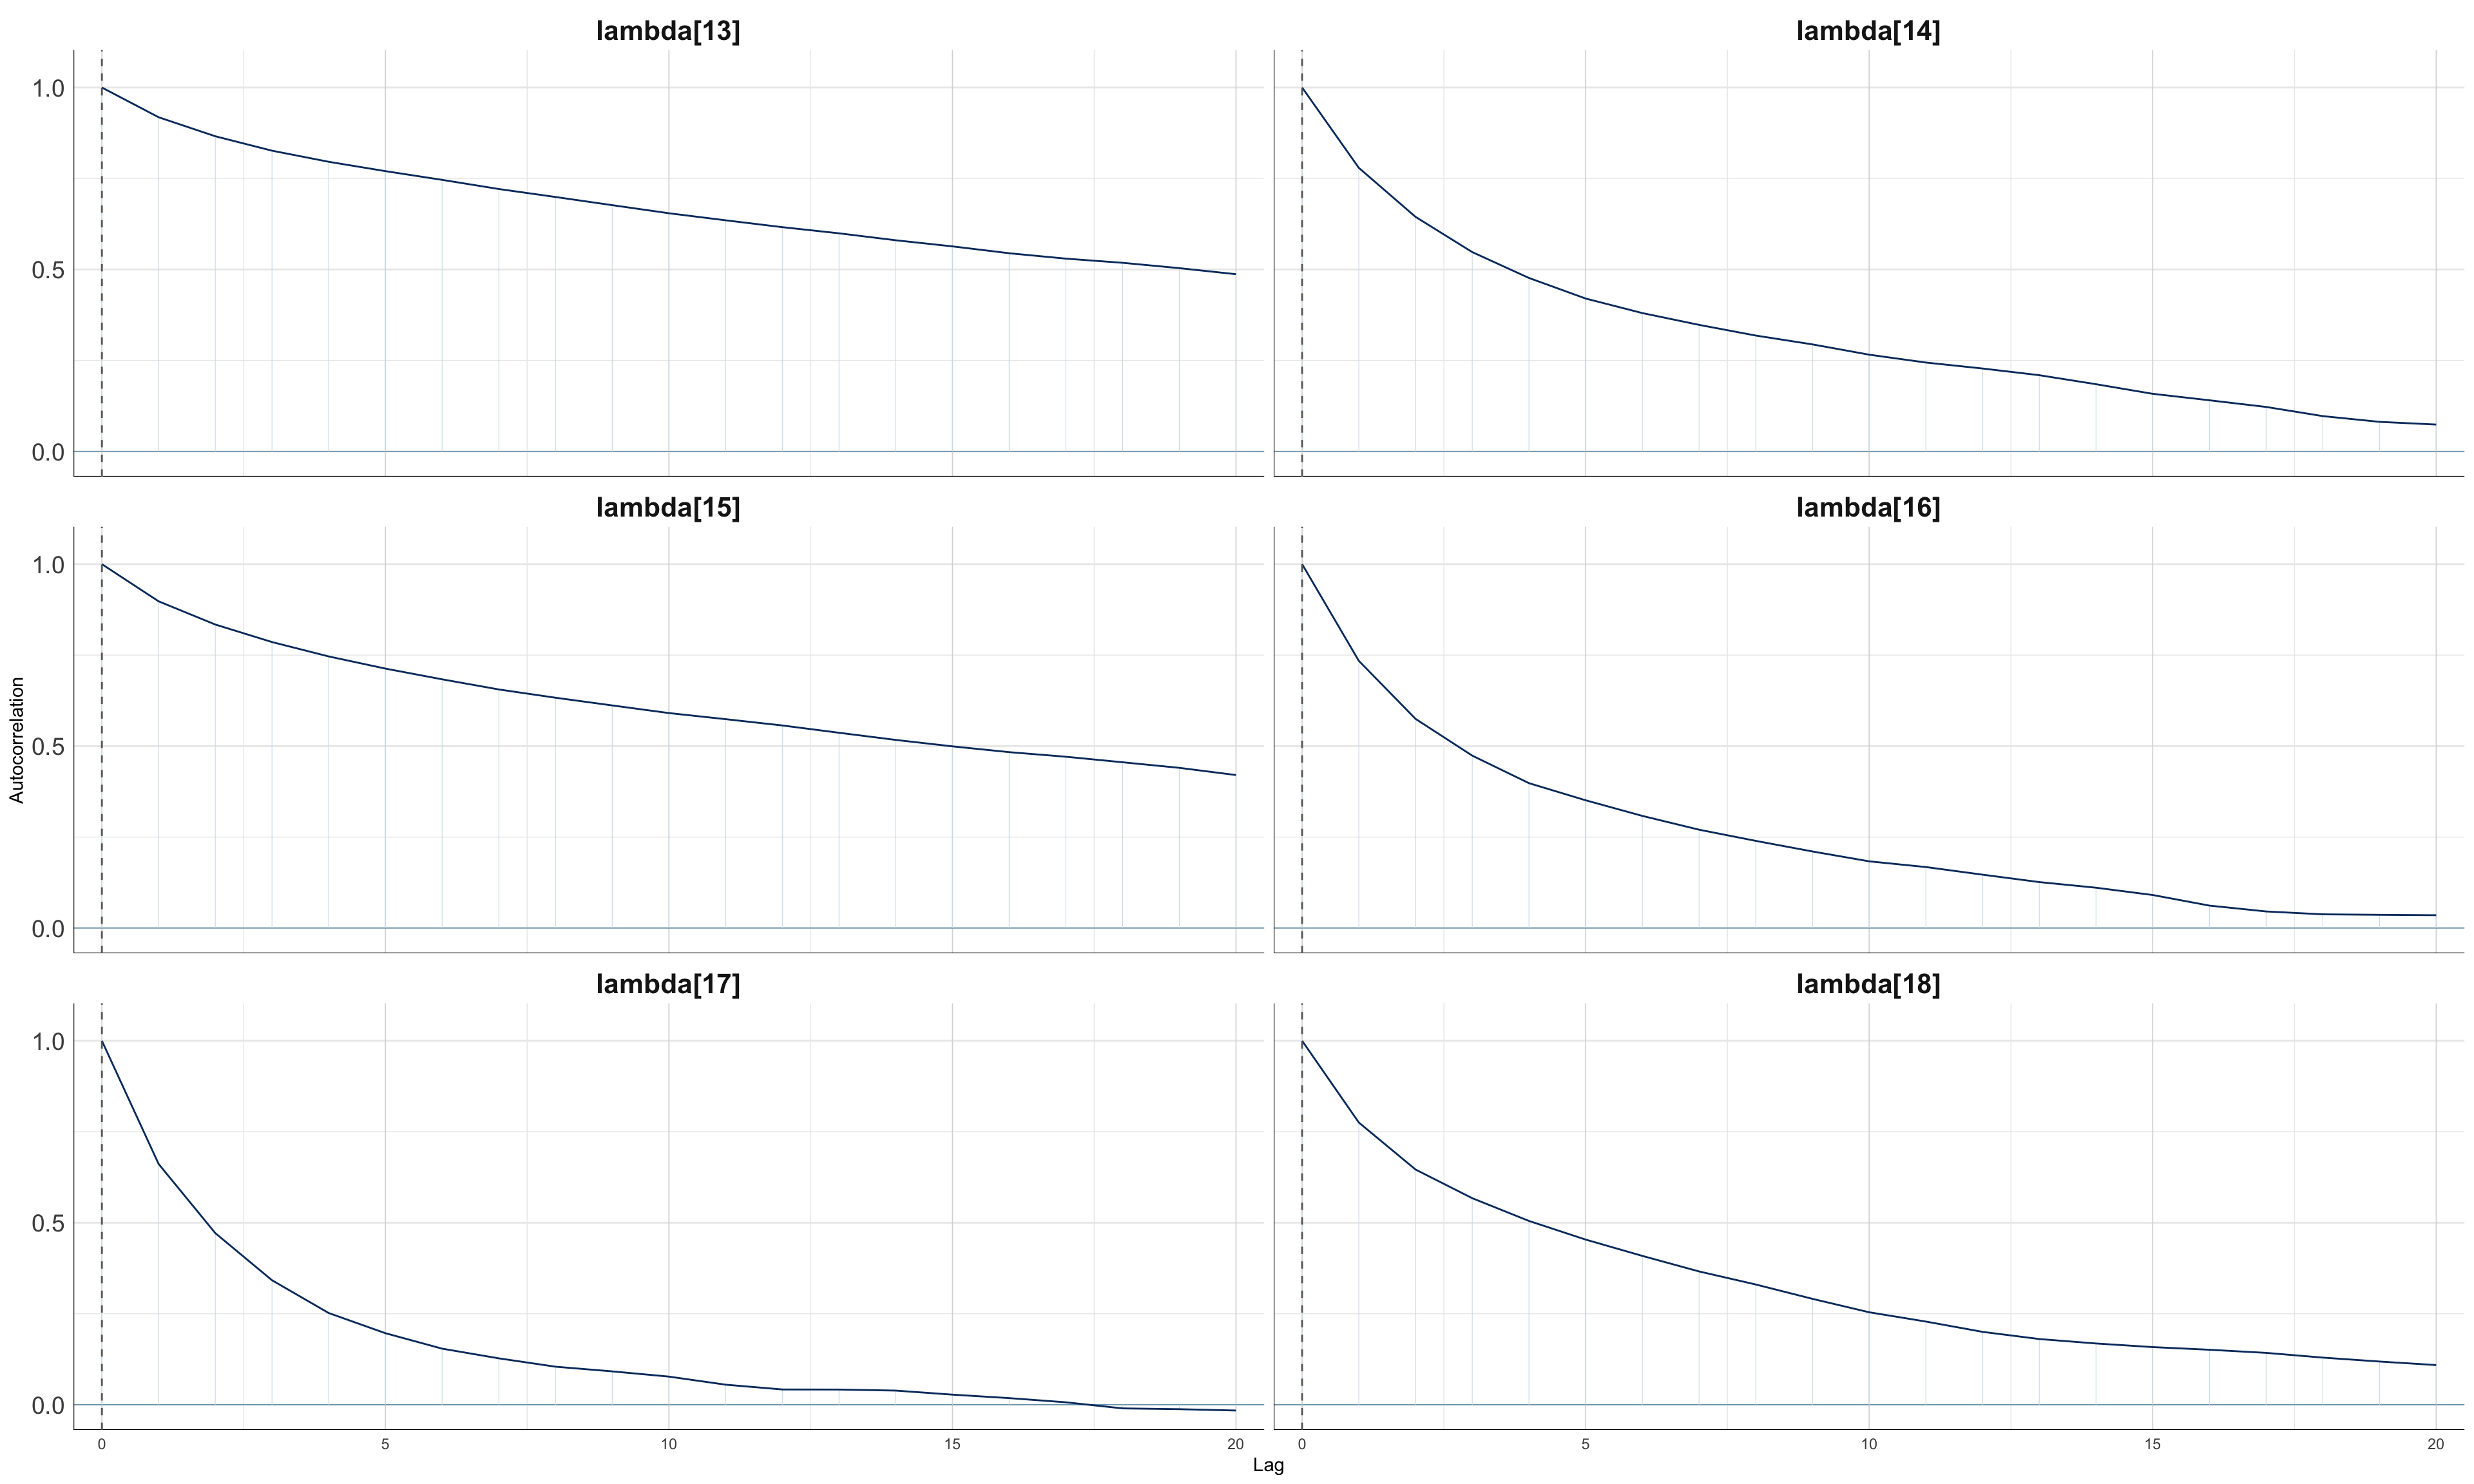
\includegraphics[width=\linewidth]{img/horseshoe_model/acf_lambda_chain3_3.png}
    \caption{Group 3.}
  \end{subfigure}\hfill
  \begin{subfigure}[t]{0.48\linewidth}
    \centering
    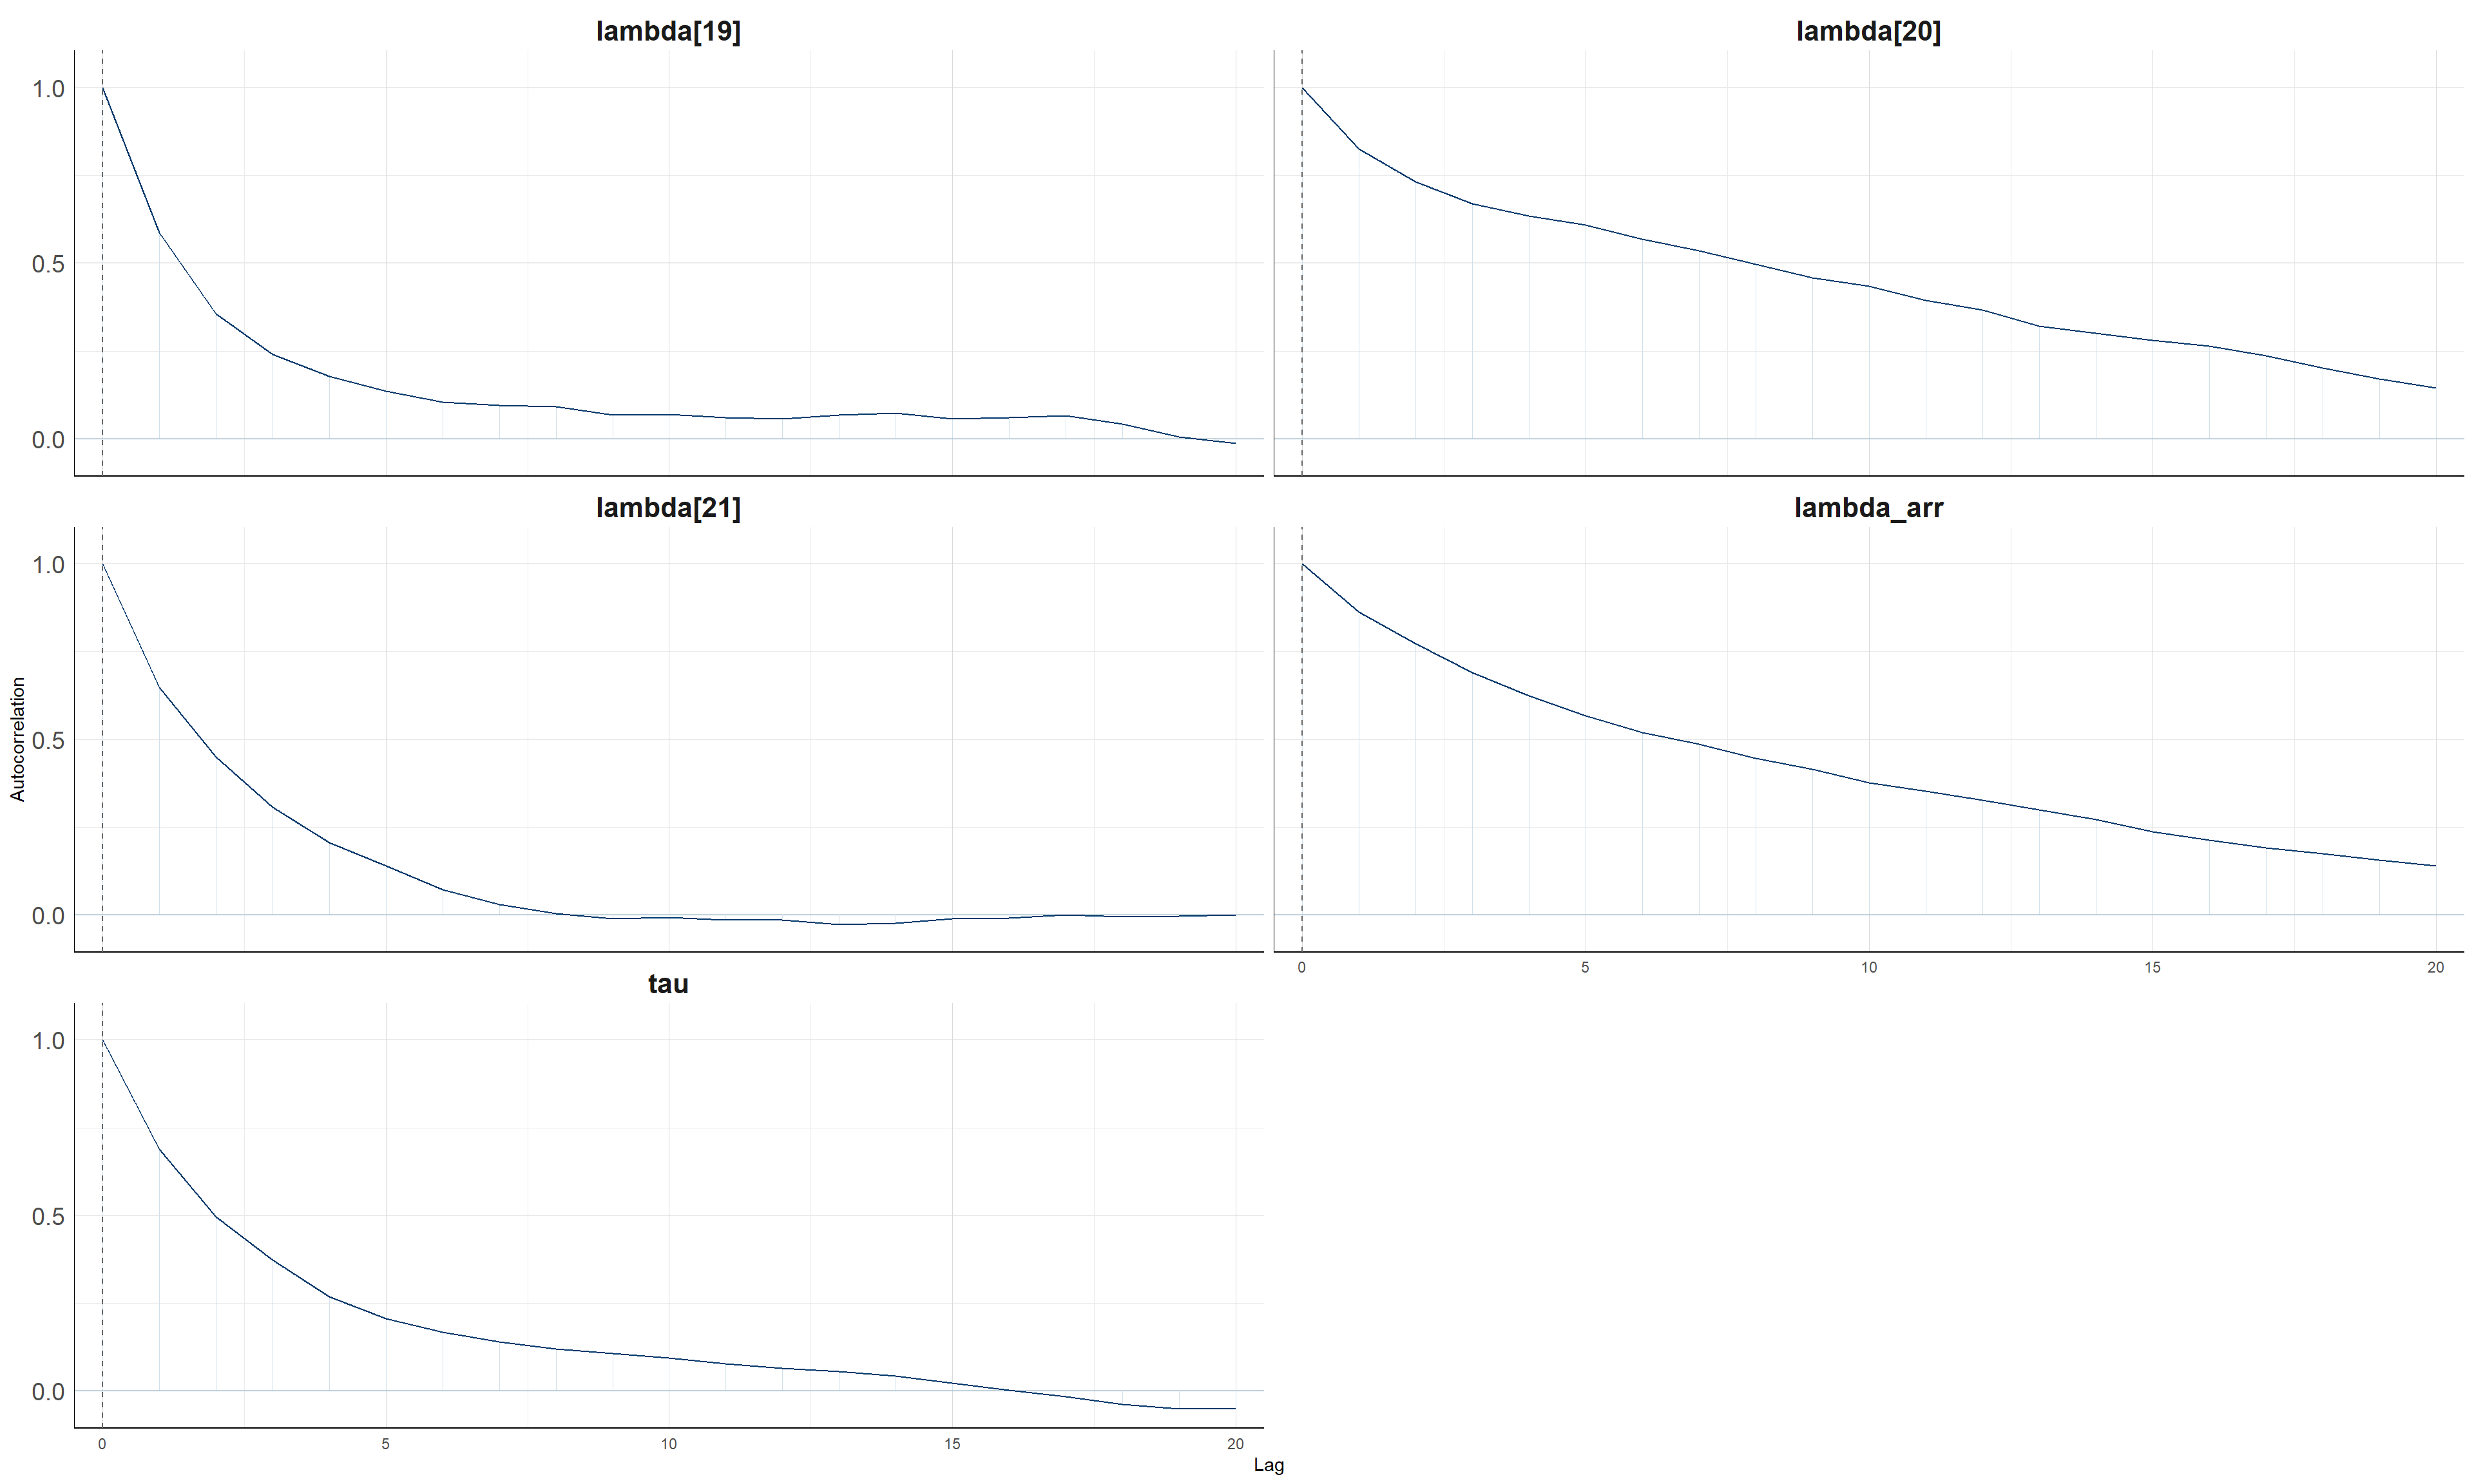
\includegraphics[width=\linewidth]{img/horseshoe_model/acf_lambda_chain3_4.png}
    \caption{Group 4.}
  \end{subfigure}\hfill
  \caption{Autocorrelation of the scales $\lambda_j$, chain 3.}
  \label{fig:hs_acf_lambda_3}
\end{figure}

\subsection*{Gelman--Rubin and effective sample sizes}
\begin{table}[htbp]
\centering\small
\caption{Regression coefficients: potential scale reduction factors and effective sample sizes.}
\label{tab:hs-psrf-beta}
\begin{tabular}{l S[table-format=1.2] S[table-format=1.2] S[table-format=5.0]}
\toprule
Parameter & {Point est.} & {Upper C.I.} & {ESS} \\
\midrule
$\beta_{1}$ (Seat comfort) & 1.00 & 1.00 & 7252 \\
$\beta_{2}$ (Dep/Arr time convenient) & 1.00 & 1.00 & 17305 \\
$\beta_{3}$ (Food and drink) & 1.00 & 1.00 & 7253 \\
$\beta_{4}$ (Gate location) & 1.00 & 1.00 & 19441 \\
$\beta_{5}$ (Inflight wifi service) & 1.00 & 1.00 & 11754 \\
$\beta_{6}$ (Inflight entertainment) & 1.00 & 1.00 & 16866 \\
$\beta_{7}$ (Online support) & 1.00 & 1.00 & 10699 \\
$\beta_{8}$ (Ease of Online booking) & 1.00 & 1.00 & 7660 \\
$\beta_{9}$ (On-board service) & 1.00 & 1.00 & 15288 \\
$\beta_{10}$ (Leg room service) & 1.00 & 1.00 & 19144 \\
$\beta_{11}$ (Baggage handling) & 1.00 & 1.00 & 11739 \\
$\beta_{12}$ (Checkin service) & 1.00 & 1.00 & 17602 \\
$\beta_{13}$ (Cleanliness) & 1.00 & 1.00 & 11220 \\
$\beta_{14}$ (Online boarding) & 1.00 & 1.00 & 12963 \\
$\beta_{15}$ (Age) & 1.00 & 1.00 & 18345 \\
$\beta_{16}$ (Flight Distance) & 1.00 & 1.00 & 23187 \\
$\beta_{17}$ (Class: Eco Plus) & 1.00 & 1.00 & 23539 \\
$\beta_{18}$ (Class: Business) & 1.00 & 1.00 & 4767 \\
$\beta_{19}$ (log(1+Departure Delay)) & 1.00 & 1.00 & 16674 \\
$\beta_{20}$ (Personal Travel) & 1.00 & 1.00 & 3813 \\
$\beta_{21}$ (disloyal Customer) & 1.00 & 1.00 & 7952 \\
$\beta_0$ (Intercept) & 1.00 & 1.00 & 3412 \\
$\beta_{\text{mid}}$ (Mid-flight delay) & 1.00 & 1.00 & 23618 \\
\bottomrule
\end{tabular}
\end{table}

\begin{table}[htbp]
\centering\small
\caption{Scale parameters: potential scale reduction factors and effective sample sizes.}
\label{tab:hs-psrf-lambda}
\begin{tabular}{l S[table-format=1.2] S[table-format=1.2] S[table-format=5.0]}
\toprule
Parameter & {Point est.} & {Upper C.I.} & {ESS} \\
\midrule
$\lambda_{1}$ (Seat comfort) & 1.01 & 1.01 & 4488 \\
$\lambda_{2}$ (Dep/Arr time convenient) & 1.02 & 1.02 & 3762 \\
$\lambda_{3}$ (Food and drink) & 1.10 & 1.12 & 1388 \\
$\lambda_{4}$ (Gate location) & 1.02 & 1.03 & 4882 \\
$\lambda_{5}$ (Inflight wifi service) & 1.03 & 1.04 & 3382 \\
$\lambda_{6}$ (Inflight entertainment) & 1.02 & 1.02 & 4499 \\
$\lambda_{7}$ (Online support) & 1.01 & 1.01 & 4077 \\
$\lambda_{8}$ (Ease of Online booking) & 1.02 & 1.03 & 2452 \\
$\lambda_{9}$ (On-board service) & 1.01 & 1.01 & 3662 \\
$\lambda_{10}$ (Leg room service) & 1.21 & 1.31 & 2103 \\
$\lambda_{11}$ (Baggage handling) & 1.03 & 1.04 & 3177 \\
$\lambda_{12}$ (Checkin service) & 1.04 & 1.05 & 3822 \\
$\lambda_{13}$ (Cleanliness) & 1.04 & 1.04 & 2497 \\
$\lambda_{14}$ (Online boarding) & 1.10 & 1.11 & 2432 \\
$\lambda_{15}$ (Age) & 1.08 & 1.11 & 2108 \\
$\lambda_{16}$ (Flight Distance) & 1.00 & 1.00 & 2753 \\
$\lambda_{17}$ (Class: Eco Plus) & 1.02 & 1.02 & 3341 \\
$\lambda_{18}$ (Class: Business) & 1.03 & 1.03 & 3262 \\
$\lambda_{19}$ (log(1+Departure Delay)) & 1.05 & 1.06 & 2458 \\
$\lambda_{20}$ (Personal Travel) & 1.01 & 1.02 & 2919 \\
$\lambda_{21}$ (disloyal Customer) & 1.05 & 1.06 & 2755 \\
$\lambda_{\text{mid}}$ (Mid-flight delay) & 1.03 & 1.04 & 3422 \\
$\tau$ (global scale) & 1.00 & 1.00 & 4515 \\
\bottomrule
\end{tabular}
\end{table}

\noindent Every coefficient has a potential scale reduction factor of
$1.00$ and an effective sample size in the thousands, the lowest being the
intercept at \num{3412}. The scale parameters are less well behaved, as
expected: their effective sample sizes run from \num{1388} to \num{4882}, and
three local scales sit at or above the conventional $1.1$ threshold ---
$\lambda_{10}$ (\emph{Leg room service}) at $1.21$ with an upper limit of
$1.31$, $\lambda_{3}$ (\emph{Food and drink}) at $1.10$, and $\lambda_{14}$
(\emph{Online boarding}) at $1.10$. We report this rather than smooth it over.
The quantity these feed into is the shrinkage weight
$\kappa_j = 1/(1+\lambda_j^2)$, which is a bounded, monotone transformation of
$\lambda_j$, and the corresponding coefficients $\beta_3$, $\beta_{10}$ and
$\beta_{14}$ have themselves converged cleanly (PSRF $1.00$, ESS \num{7253},
\num{19144} and \num{12963}). The conclusions of Section~\ref{sec:regression}
rest on the coefficients and on the broad signal/noise separation, not on the
third decimal of any single $\kappa_j$, and
Section~\ref{sec:sens-horseshoe} shows the verdicts are stable across a
hundred-fold change in the global scale. The global scale $\tau$ itself mixes
well (PSRF $1.00$, ESS \num{4515}).

% ==================================================================
% BAS vs. Horseshoe --- includable section fragment
% Meant to be \input{} / \include{} inside a larger document.
%
% Parent preamble must load: amsmath, amssymb, graphicx, booktabs,
%   siunitx  (and set \sisetup{table-format=1.3,round-mode=places,
%   round-precision=3} or equivalent).
% Figures fig1.png / fig2.png must sit where \graphicspath can find them.
% ==================================================================

\section{Feature selection cross-check with BAS}
\noindent
After fitting our feature-selection model based on a horseshoe prior, we
would like to compare it with a Bayesian Adaptive Sampling (BAS) model in
order to verify whether the two methods agree on which covariates are more
useful in explaining the target variable.

With $23$ predictors, $2^{23}\approx 8.4$ million candidate models are far
too many to enumerate exhaustively, so we use \texttt{method = "MCMC"} in
BAS to stochastically search the model space. A later section assesses
whether this search suffers from instability or not.

Table~\ref{tab:bas-top} reports the marginal posterior inclusion
probabilities $P(\beta_j \neq 0 \mid Y)$ for every predictor, together with
the five highest-probability models returned by the search and their
summary statistics (Bayes factor, posterior probability, $R^2$,
dimension and log marginal likelihood).

\begin{table}[htbp]
\centering
\footnotesize
\caption{Marginal posterior inclusion probabilities and the top five
models identified by the BAS MCMC search. A value of $1.000$/$0.000$ in a
model column indicates the predictor is included/excluded in that model.}
\label{tab:bas-top}
\begin{tabular}{l S S S S S S}
\toprule
& {$P(\beta\!\neq\!0\mid Y)$} & {Model 1} & {Model 2} & {Model 3} & {Model 4} & {Model 5}\\
\midrule
Intercept            & 1.000 & 1.000 & 1.000 & 1.000 & 1.000 & 1.000\\
seat\_comfort        & 0.803 & 1.000 & 1.000 & 1.000 & 1.000 & 0.000\\
time\_convenient     & 0.973 & 1.000 & 1.000 & 1.000 & 1.000 & 1.000\\
food\_drink          & 0.500 & 1.000 & 0.000 & 1.000 & 0.000 & 0.000\\
gate\_location       & 0.037 & 0.000 & 0.000 & 0.000 & 0.000 & 0.000\\
wifi                 & 0.049 & 0.000 & 0.000 & 0.000 & 0.000 & 0.000\\
entertainment        & 1.000 & 1.000 & 1.000 & 1.000 & 1.000 & 1.000\\
online\_support      & 0.220 & 0.000 & 0.000 & 0.000 & 0.000 & 0.000\\
ease\_booking        & 0.954 & 1.000 & 1.000 & 1.000 & 1.000 & 1.000\\
onboard\_service     & 0.996 & 1.000 & 1.000 & 1.000 & 1.000 & 1.000\\
legroom              & 0.965 & 1.000 & 1.000 & 1.000 & 1.000 & 1.000\\
baggage              & 0.073 & 0.000 & 0.000 & 0.000 & 0.000 & 0.000\\
checkin              & 0.986 & 1.000 & 1.000 & 1.000 & 1.000 & 1.000\\
cleanliness          & 0.310 & 0.000 & 0.000 & 0.000 & 0.000 & 0.000\\
online\_boarding     & 0.029 & 0.000 & 0.000 & 0.000 & 0.000 & 0.000\\
Age\_std             & 0.037 & 0.000 & 0.000 & 0.000 & 0.000 & 0.000\\
FlightDist\_std      & 0.035 & 0.000 & 0.000 & 0.000 & 0.000 & 0.000\\
Class\_EcoPlus       & 0.029 & 0.000 & 0.000 & 0.000 & 0.000 & 0.000\\
Class\_Business      & 0.993 & 1.000 & 1.000 & 1.000 & 1.000 & 1.000\\
logdep\_std          & 0.092 & 0.000 & 0.000 & 0.000 & 0.000 & 0.000\\
TypeTravel\_Personal & 0.451 & 0.000 & 0.000 & 1.000 & 1.000 & 1.000\\
CustType\_disloyal   & 1.000 & 1.000 & 1.000 & 1.000 & 1.000 & 1.000\\
logmid\_delay        & 0.031 & 0.000 & 0.000 & 0.000 & 0.000 & 0.000\\
\midrule
BF        & {NA} & 1.000    & 0.574    & 0.477    & 0.369    & 0.268\\
PostProbs & {NA} & 0.128    & 0.071    & 0.059    & 0.048    & 0.033\\
$R^2$     & {NA} & 0.426    & 0.421    & 0.430    & 0.425    & 0.420\\
dim       & {NA} & 11.000   & 10.000   & 12.000   & 11.000   & 10.000\\
logmarg   & {NA} & -516.838 & -517.392 & -517.578 & -517.835 & -518.155\\
\bottomrule
\end{tabular}
\end{table}

% ==================================================================
\section{Parameter-space convergence}


% ==================================================================
We now test the goodness of the MCMC search over the parameter space
executed by BAS.

% ------------------------------------------------------------------
\subsection*{Convergence within one run}
% ------------------------------------------------------------------
BAS reports two independent estimates of each posterior inclusion
probability:
\begin{itemize}
  \item \texttt{probne0.RB}: takes the set of distinct visited models that
  contain variable $j$, uses their marginal likelihoods, renormalises and
  sums the mass of those models;
  \item \texttt{probne0.MCMC}: the raw fraction of iterations the chain
  spent in some model containing variable $j$.
\end{itemize}
If the chain has converged, the two estimates should agree closely.

The correlation between the two estimates is $0.9999$ and the maximum
absolute difference is $0.014$: the points sit essentially on the diagonal
(Figure~\ref{fig:conv}), the sign that this run has converged.

\begin{figure}[htbp]
\centering
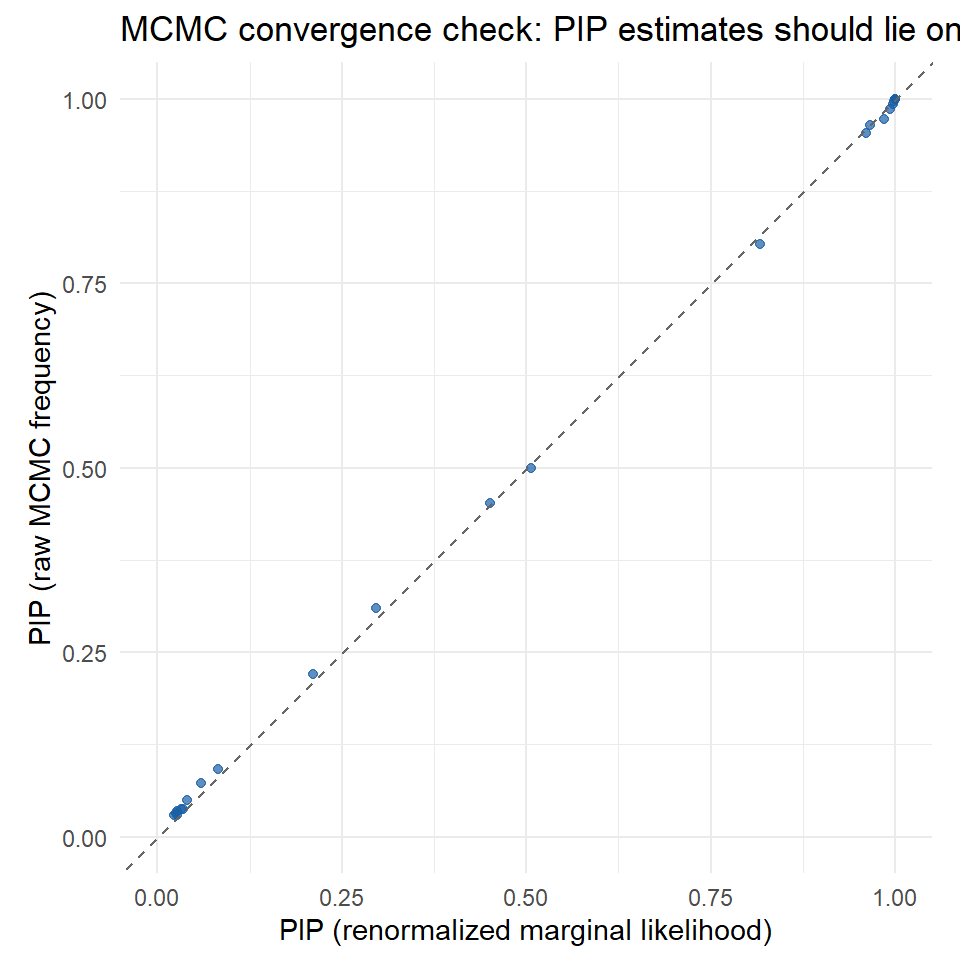
\includegraphics[width=0.6\textwidth]{img/bas_crosscheck/BAS_PIP_comparison.png}
\caption{MCMC convergence check. Renormalised-marginal-likelihood
inclusion probabilities (x-axis) against raw MCMC-frequency inclusion
probabilities (y-axis); points lying on the dashed diagonal indicate the
two estimates agree.}
\label{fig:conv}
\end{figure}

% ------------------------------------------------------------------
\subsection*{Stability across seeds}
% ------------------------------------------------------------------
We refit the identical model twice more with different random seeds and
compare the posterior inclusion probabilities (PIPs) to check whether they
agree. Table~\ref{tab:seeds} lists the predictors with the largest spread,
ordered by the range across the three seeds.

\begin{table}[htbp]
\centering
\caption{Posterior inclusion probabilities across three random seeds, with
the range (max $-$ min) per predictor. Only the eight most variable
predictors are shown.}
\label{tab:seeds}
\begin{tabular}{l S S S S}
\toprule
term & {seed123} & {seed1} & {seed2} & {range}\\
\midrule
seat\_comfort        & 0.803 & 0.841 & 0.826 & 0.038\\
food\_drink          & 0.500 & 0.533 & 0.511 & 0.033\\
online\_support      & 0.220 & 0.228 & 0.204 & 0.024\\
cleanliness          & 0.310 & 0.297 & 0.316 & 0.019\\
TypeTravel\_Personal & 0.451 & 0.439 & 0.457 & 0.017\\
legroom              & 0.965 & 0.951 & 0.959 & 0.013\\
time\_convenient     & 0.973 & 0.979 & 0.983 & 0.011\\
baggage              & 0.073 & 0.065 & 0.064 & 0.009\\
\bottomrule
\end{tabular}
\end{table}

% ------------------------------------------------------------------
\subsection*{BIC prior as a robustness check}
% ------------------------------------------------------------------
We try another prior on the $\beta$ coefficients: if the search is stable,
the effect of the prior should vanish once the number of iterations is
large enough. Table~\ref{tab:bic} compares the $g$-prior PIPs with those
obtained under a BIC-based prior.

\begin{table}[htbp]
\centering
\caption{Posterior inclusion probabilities under the $g$-prior and the
BIC-based prior, with the absolute difference per predictor (six most
affected predictors shown).}
\label{tab:bic}
\begin{tabular}{l S S S}
\toprule
term & {g\_prior} & {BIC} & {abs\_diff}\\
\midrule
online\_support & 0.220 & 0.224 & 0.004\\
cleanliness     & 0.310 & 0.314 & 0.004\\
seat\_comfort   & 0.803 & 0.801 & 0.002\\
food\_drink     & 0.500 & 0.498 & 0.002\\
ease\_booking   & 0.954 & 0.952 & 0.002\\
legroom         & 0.965 & 0.967 & 0.002\\
\bottomrule
\end{tabular}
\end{table}

With $100{,}000$ MCMC iterations, PIPs move by at most $0.038$ across the
three seeds and by at most $0.004$ between the $g$-prior and the BIC-based
prior. Given the number of MCMC iterations, the search proves itself to be
stable.

% ==================================================================
\section{BAS vs.\ Horseshoe: model comparison}
\label{app:bas_vs_hs}

% ==================================================================
Finally, we compare the models selected by the two approaches and check on
which coefficients they agree and on which they do not. Figure~\ref{fig:cmp}
plots each predictor's BAS inclusion probability against the horseshoe's
$1-\kappa_j$ shrinkage measure, colouring predictors by whether the two
methods make the same signal/noise call.

\begin{figure}[htbp]
\centering
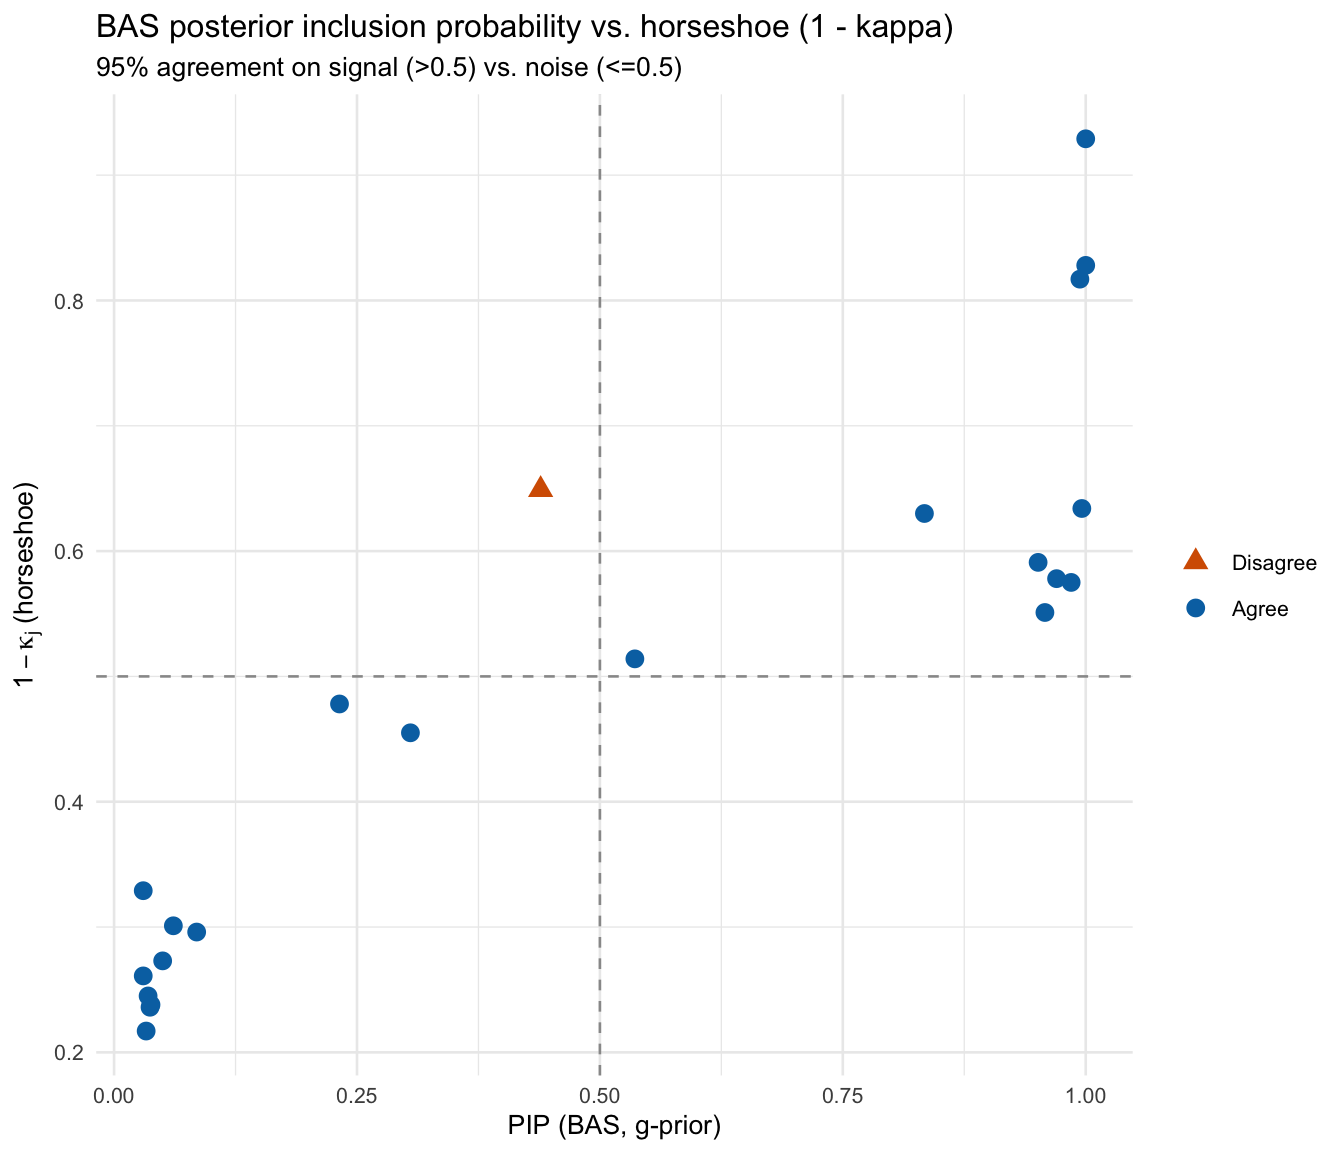
\includegraphics[width=0.75\textwidth]{img/bas_crosscheck/bas_vs_horseshoe_comparison.png}
\caption{BAS posterior inclusion probability (x-axis) against the
horseshoe's $1-\kappa_j$ (y-axis). Dashed lines mark the $0.5$ signal/noise
cutoff for each method; green points denote agreement, the red point
denotes the single disagreement.}
\label{fig:cmp}
\end{figure}

91\% of the 22 predictors get the same signal/noise call from BAS's
model-space search and from the horseshoe's continuous shrinkage --
two structurally different estimation strategies (discrete model
averaging vs.\ a single shrinkage prior) landing on the same handful
of variables. The two disagreements are genuine borderline cases in
both methods: \texttt{Personal Travel} (PIP 0.439, $\kappa = 0.353$)
sits just on opposite sides of each method's 0.5 cutoff, and
\texttt{Food and drink} (PIP $\approx 0.50$, $\kappa = 0.489$) sits
essentially on the cutoff for both methods and flips across MCMC
seeds (Table~18) -- not a real contradiction between the two
approaches, but two variables where the signal is genuinely too weak
to classify with confidence.
\end{appendices}

\printbibliography
\end{document}
